\documentclass[11pt, a4paper, openright]{book}

\usepackage{bm}
\usepackage[utf8]{inputenc}
\usepackage[italian]{babel}
\usepackage{amsmath, amssymb}
\usepackage{amsthm}
\usepackage{graphicx}
\usepackage{booktabs}
\usepackage{geometry}
\geometry{a4paper, top=2.5cm, bottom=2.5cm, left=2.5cm, right=2.5cm}
\usepackage{caption}
\captionsetup{justification=centering}
\usepackage{float}
\usepackage[hidelinks]{hyperref}
\usepackage{subcaption}
\usepackage{verbatim}
\usepackage{enumitem}
\usepackage{yhmath}
\usepackage{derivative}
\usepackage{physics}

\usepackage{selectp}

% \outputonly{111-150}

\setcounter{tocdepth}{3} 
\setcounter{secnumdepth}{3}

\theoremstyle{plain}
\newtheorem{theorem}{Teorema}[section]
\newtheorem{lemma}[theorem]{Lemma}
\newtheorem{corollario}[theorem]{Corollario}

\theoremstyle{definition}
\newtheorem{definizione}{Definizione}[section]

\begin{document}

\begin{titlepage}
    \centering
    \vspace*{4cm}
    
    \Huge
    \textbf{Corso di Meccanica}
    
    \vspace{0.5cm}
    \LARGE
    Appunti ed Esempi
    
    \vspace{1.5cm}
    
    \textit{Basato sulle lezioni del} \\
    \Large \textbf{Prof. R. Mazzarello}
    
    \vfill
    
    \rule{\linewidth}{0.5pt}
    \vspace{0.5cm}
    
    \large
    Autore: \textbf{Liam Ferretti} \\
    \today
    
\end{titlepage}

\tableofcontents

% INSERIRE FORZE CENTRALI A SIMMETRIA SFERICA E FORZE CENTRALI A SIMMETRIA CILINDRICA

\chapter{Introduzione}
\section{Sistemi di coordinate}
\subsection{Coordinate cartesiane ortogonali}
Nel sistema di coordinate cartesiane un punto è individuato da 3 coordinate:
\begin{equation}
    \vec{r} = \overline{OP} = (x, y ,z)
\end{equation}

\subsection{Coordinate polari}
Si definisce:
\begin{itemize}
    \item $r := |\vec{r}| \Rightarrow \vec{r} = r \cdot \hat{u}_r$
    \item $\theta$ l'angolo fra $\vec{r}$ e l'asse polare $(x)$
\end{itemize}
Allora:
\begin{equation}
    \begin{cases}
    x = r\cos\theta \\
    y = r\sin\theta \\
\end{cases} \Rightarrow \begin{cases}
    r = \sqrt{x^2 + y^2} \\
    \theta =  \arctan(\frac{y}{x}) + c\footnotemark\\
\end{cases}
\end{equation}
\footnotetext{c dipende dal quadrante in cui ci si trova}

Per ricavare i versori della base locale, si esprime il vettore posizione $\vec{r} = (r\cos\theta)\hat{\imath} + (r\sin\theta)\hat{\jmath}$ e si normalizzano le derivate parziali rispetto alle coordinate:
\begin{itemize}
    \item Il versore rispetto a $r$:
        \begin{align}
            \hat{u}_r = \frac{\frac{\partial \vec{r}}{\partial r}}{\left|\frac{\partial \vec{r}}{\partial r}\right|} & = \frac{(\cos\theta, \sin\theta)}{\sqrt{\cos^2\theta + \sin^2\theta}} \\
            & = (\cos\theta, \sin\theta)
        \end{align}
    \item Il versore rispetto a $\theta$:
        \begin{align}
            \hat{u}_\theta = \frac{\frac{\partial \vec{r}}{\partial \theta}}{\left|\frac{\partial \vec{r}}{\partial \theta}\right|} & = \frac{(-r\sin\theta, r\cos\theta)}{\sqrt{r^2\sin^2\theta + r^2\cos^2\theta}} \\ 
            & = \frac{(-r\sin\theta, r\cos\theta)}{r} \\ 
            & = (-\sin\theta, \cos\theta)
        \end{align}
\end{itemize}

Inoltre derivando i versori, segue che:

\[\frac{d\hat{u}_r}{d\theta} = (-\sin\theta, \cos\theta) = \hat{u}_\theta\]
\[\frac{d\hat{u}_\theta}{d\theta} = (-\cos\theta, -\sin\theta) = -(\cos\theta, \sin\theta) = -\hat{u}_r\]

\subsection{Coordinate cilindriche}

Le coordinate cilindriche $(\rho, \varphi, z)$ estendono le polari aggiungendo la quota $z$.
\begin{itemize}
    \item $\rho$: distanza dalla proiezione del punto sul piano $xy$ all'origine.
    \item $\varphi$: angolo azimutale (corrisponde al $\theta$ delle polari).
    \item $z$: quota (identica alla coordinata cartesiana).
\end{itemize}

\[
\begin{cases}
    x & = \rho\cos\varphi \\
    y & = \rho\sin\varphi \\
    z & = z
\end{cases} \Rightarrow \begin{cases}
    \rho & = \sqrt{x^2 + y^2} \\
    \varphi & =  \arctan(\frac{y}{x}) + c\\
    z & = z
\end{cases}
\]
Il vettore posizione è $\vec{r} = (\rho\cos\varphi)\hat{\imath} + (\rho\sin\varphi)\hat{\jmath} + z\hat{k}$, si possono quindi trovare i 3 versori:
\begin{itemize}
    \item Il versore rispetto a $\rho$:
        \begin{align}
            \hat{u}_\rho = \frac{\frac{\partial \vec{r}}{\partial \rho}}{|\frac{\partial \vec{r}}{\partial \rho}|} & = \frac{(\cos\varphi, \sin\varphi, 0)}{\sqrt{\cos^2\varphi + \sin^2\varphi}} \\ 
            & = (\cos\varphi, \sin\varphi, 0)
        \end{align}
    \item Il versore rispetto a $\varphi$:
        \begin{align}
            \hat{u}_\varphi = \frac{\frac{\partial \vec{r}}{\partial \varphi}}{|\frac{\partial \vec{r}}{\partial \varphi}|} & = \frac{(-\rho\sin\varphi,\rho\cos\varphi, 0)}{\sqrt{\rho^2\sin^2\varphi + \rho^2\cos^2\varphi}} \\
            & = \frac{(-\rho\sin\varphi,\rho\cos\varphi, 0)}{\rho} \\ 
            & = (-\sin\varphi,\cos\varphi, 0)
        \end{align}
    \item Il versore rispetto a $z$:
        \[\hat{u}_z = \frac{\frac{\partial \vec{r}}{\partial z}}{|\frac{\partial \vec{r}}{\partial z}|} = (0, 0, 1) = \hat{k}\]
\end{itemize}

\subsection{Coordinate sferiche}
In questo sistema un punto è individuato da $(r, \theta, \varphi)$, dove $\theta$ è l'angolo zenitale (colatitudine) e $\varphi$ l'angolo azimutale.
\[
\begin{cases}
    x & = r\sin\theta\cos\varphi \\
    y & = r\sin\theta\sin\varphi \\
    z & = r\cos\theta
\end{cases} 
\Rightarrow 
\begin{cases}
    r & = \sqrt{x^2 + y^2 + z^2} \\
    \theta & =  \arccos(\frac{z}{r}) = \arccos(\frac{z}{\sqrt{x^2 + y^2 + z^2}})\\
    \varphi & = \arctan(\frac{y}{x}) + c
\end{cases}
\]
Il vettore posizione è:
\[\vec{r} = (r\sin\theta\cos\varphi)\hat{\imath} + (r\sin\theta\sin\varphi)\hat{\jmath} + (r\cos\theta)\hat{k}\]
applicando il metodo delle derivate parziali, si trovano i versori:

\begin{itemize}
    \item Il versore rispetto a $r$:
        \begin{align}
            \hat{u}_r = \frac{\partial \vec{r}}{\partial r} & = \frac{(\sin\theta\cos\varphi, \sin\theta\sin\varphi, \cos\theta)}{\sqrt{\sin^2\theta\cos^2\varphi + \sin^2\theta\sin^2\varphi + \cos^2\theta}} \\
            & = (\sin\theta\cos\varphi, \sin\theta\sin\varphi, \cos\theta)
        \end{align}
    \item Il versore rispetto a $\theta$:
        \begin{align}
            \hat{u}_\theta = \frac{\partial \vec{r}}{\partial \theta} & = \frac{(r\cos\theta\cos\varphi, r\cos\theta\sin\varphi, -r\sin\theta)}{\sqrt{r^2\cos^2\theta\cos^2\varphi + r^2\cos^2\theta\sin^2\varphi + r^2\sin^2\theta}} \\
                & = \frac{(r\cos\theta\cos\varphi, r\cos\theta\sin\varphi, -r\sin\theta)}{r}  \\
                & = (\cos\theta\cos\varphi, \cos\theta\sin\varphi, -\sin\theta)
        \end{align}
    \item Il versore rispetto a $\varphi$:
        \begin{align}
            \hat{u}_\varphi = \frac{\partial \vec{r}}{\partial \varphi} & = \frac{(-r\sin\theta\sin\varphi, r\sin\theta\cos\varphi, 0)}{\sqrt{r^2\sin^2\theta\sin^2\varphi + r^2\sin^2\theta\cos^2\varphi}} \\
            & = \frac{(-r\sin\theta\sin\varphi, r\sin\theta\cos\varphi, 0)}{r\sin\theta} \\
            & = (-\sin\varphi, \cos\varphi, 0)
        \end{align}
\end{itemize}

\chapter{Cinematica}
\section{Equazione del moto}
\subsection{Equazione vettoriale del moto}
Si può definire l'equazione vettoriale del moto, nel seguente modo
\[\vec{r} = \vec{r}(t)\]
e si assume che questa funzione, che associa al tempo una posizione, appartenga alle funzioni $\mathcal{C}^2$, quindi derivabili due volte con derivate continue.
\subsection{Rappresentazione intrinseca della traiettoria}
Spesso conviene separare gli aspetti geometrici da quelli cinematici, e per far ciò si introduce una ascissa curvilinea, associata a un punto $P$ sulla curva, quindi si può approssimare la curva come una serie di spezzate poligonali, attraverso un limite del numero di spezzate che tende a $+\infty$ con lunghezza $l \rightarrow 0$.

Quindi si definisce:
\[|S| := \text{lunghezza di } \wideparen{\Omega P}; \quad \text{con segno } \begin{cases}
    + & \text{se P si trova dopo $\Omega$} \\
    - & \text{se P si trova prima di $\Omega$}
\end{cases}
\]
Segue che si possono definire due funzioni:
\begin{itemize}
    \item equazione della traiettoria:
    \[\vec{r} = \vec{r}(s)\]
    \item legge oraria:
    \[s = s(t)\]
\end{itemize}
Segue quindi che:
\[\vec{r} = \vec{r}(s(t))\]

\newpage

\section{Velocità}
\subsection{Velocità media}
La velocità media si definisce come:
\[\vec{v}_m = \frac{\Delta \vec{r}}{\Delta t}\]
dove per $\Delta \vec{r}$ lo spostamento tra i due punti considerati, e si definisce come:
\[\Delta \vec{r} = \vec{r}(t + \Delta t) - \vec{r}(t)\]

\subsection{Velocità istantanea}
Se si considera la velocità media, in cui:
\[\Delta t \rightarrow 0,\]
allora si sta misurando la velocità istantanea (o semplicemente velocità), quindi:
\[\vec{v} = \lim_{\Delta t \rightarrow 0} \frac{\Delta \vec{r}}{\Delta t} = \frac{d\vec{r}}{dt}\]
La velocità si può rappresentare in relazione al sistema di coordinate scelto:
\begin{itemize}
    \item In coordinate cartesiane, poiché:
    \[\vec{r} = x\hat{\imath} + y\hat{\jmath} + z\hat{k}\]
    Allora derivando entrambi i lati si ottiene:
    \begin{align}
        \vec{v} & = v_x\hat{\imath} + v_y\hat{\jmath} + v_z\hat{k} \\
                & = \frac{dx}{dt}\hat{\imath} + \frac{dy}{dt}\hat{\jmath} + \frac{dz}{dt}\hat{k} \\
                & = \dot{x}\hat{\imath} + \dot{y}\hat{\jmath} + \dot{z}\hat{k} \\
                & = \dot{\vec{r}}
    \end{align}
    \item In coordinate polari, poiché:
    \[\vec{r} = r\underbrace{(\cos\theta \hat{\imath} + \sin\theta \hat{\jmath})}_{\hat{u}_r} = r\hat{u}_r\]
    Allora segue che:
    \begin{align}
        \vec{v} = \dot{\vec{r}} & = \frac{d}{dt}(r\hat{u}_r) \\
        & = \frac{dr}{dt}\hat{u}_r + r\frac{d\hat{u}_r}{dt} \\
        & = \dot{r}\hat{u}_r + r\frac{d}{dt}(\cos\theta \hat{\imath} + \sin\theta \hat{\jmath}) \\
        & = \dot{r}\hat{u}_r + r(-\dot{\theta}\sin\theta\hat{\imath} + \dot{\theta}\cos\theta\hat{\jmath}) \\
        & = \dot{r}\hat{u}_r + r\dot{\theta}\underbrace{(-\sin\theta\hat{\imath} + \cos\theta\hat{\jmath})}_{\hat{u}_\theta} \\
        & = \dot{r}\hat{u}_r + r\dot{\theta}\hat{u}_\theta
    \end{align}
    \item In coordinate sferiche, poiché:
    \[\vec{r} = (r\sin\theta\cos\varphi)\hat{\imath} + (r\sin\theta\sin\varphi)\hat{\jmath} + (r\cos\theta)\hat{k}\]
    Allora derivando componente per componente segue che:
    \begin{itemize}
        \item Derivando la componente $\hat{\imath}$:
        \begin{align}
            \frac{d}{dt}(r\sin\theta\cos\varphi) = \dot{r}\sin\theta\cos\varphi + r\dot{\theta}\cos\theta\cos\varphi - r\dot{\varphi}\sin\theta\sin\varphi
        \end{align}
        \item Derivando la componente $\hat{\jmath}$:
        \begin{align}
            \frac{d}{dt}(r\sin\theta\sin\varphi) = \dot{r}\sin\theta\sin\varphi + r\dot{\theta}\cos\theta\sin\varphi + r\dot{\varphi}\sin\theta\cos\varphi
        \end{align}
        \item Derivando la componente $\hat{k}$:
        \begin{align}
            \frac{d}{dt}(r\cos\theta) = \dot{r}\cos\theta - r\dot{\theta}\sin\theta
        \end{align}
    \end{itemize}
    Raccogliendo per le componenti segue che:
    \begin{align}
        \vec{v} & = \dot{r}(\sin\theta\cos\varphi + \sin\theta\sin\varphi + \cos\theta ) + \dot{\theta}(r\cos\theta\cos\varphi + r\cos\theta\sin\varphi - r\sin\theta) + \\
        &\quad \; + \dot{\varphi}(-r\sin\theta\sin\varphi + r\sin\theta\cos\varphi) \\
        & = \dot{r}\hat{u}_r + r\dot{\theta}\hat{u}_\theta + \dot{\varphi}(r\sin\theta)\hat{u}_\varphi
    \end{align}
    \item In coordinate cilindriche, poiché:
    \[
    \vec{r} = (\rho\cos\varphi)\hat{\imath} + (\rho\sin\varphi)\hat{\jmath} + z\hat{k} = \rho\underbrace{(\cos\varphi\hat{\imath} + \sin\varphi\hat{\jmath})}_{\hat{u}_\rho} + z\hat{k} = \rho\hat{u}_\rho + z\hat{k}
    \]
    Allora derivando rispetto al tempo segue che:
    \begin{align}
    \vec{v} = \dot{\vec{r}} & = \frac{d}{dt}(\rho\hat{u}_\rho + z\hat{k}) \\
    & = \frac{d\rho}{dt}\hat{u}_\rho + \rho\frac{d\hat{u}_\rho}{dt} + \frac{dz}{dt}\hat{k} \\
    & = \dot{\rho}\hat{u}_\rho + \rho\frac{d}{dt}(\cos\varphi \hat{\imath} + \sin\varphi \hat{\jmath}) + \dot{z}\hat{k} \\
    & = \dot{\rho}\hat{u}_\rho + \rho(-\dot{\varphi}\sin\varphi\hat{\imath} + \dot{\varphi}\cos\varphi\hat{\imath}) + \dot{z}\hat{k} \\
    & = \dot{\rho}\hat{u}_\rho + \rho\dot{\varphi}\underbrace{(-\sin\varphi\hat{\imath} + \cos\varphi\hat{\jmath})}_{\hat{u}\varphi} + \dot{z}\hat{k} \\ 
    & = \dot{\rho}\hat{u}_\rho + \rho\dot{\varphi}\hat{u}_\varphi + \dot{z}\hat{k}
    \end{align}
\end{itemize}

\newpage
\subsection{Rappresentazione intrinseca della velocità}
Sapendo che:
\[\vec{r} = \vec{r}(s(t))\]
Allora:
\[\vec{v} = \dot{\vec{r}} = \frac{d\vec{r}}{ds}\frac{ds}{dt} = \dot{s}\frac{d\vec{r}}{ds}\]
dove $\dot{s}$ si definisce come velocità scalare.

Come già visto vale che:
\[\frac{d\vec{r}}{ds} = \lim_{\Delta s \rightarrow 0} \frac{\Delta \vec{r}}{\Delta s}\]
Quindi:
\[\lim_{\Delta s \rightarrow 0} \left|\frac{\Delta\vec{r}}{\Delta s}\right| = 1\]
poiché per un $\Delta s$ che tende a 0, il vettore spostamento $(\Delta \vec{r})$ e lo spazio percorso $\Delta s$ sono uguali, infatti la curva si approssima a una retta, quindi $d\vec{r}$ e $ds$ hanno lo stesso valore.

Quindi segue che:
\[\vec{v} = \frac{d\vec{r}}{ds}\dot{s} = \dot{s}\hat{u}_t\]
dove:
\[\hat{u}_t = \frac{d\vec{r}}{ds}; \quad \text{versore tangente al moto}\]

Vale quindi che:
\[v = \sqrt{v_x^2 + v_y^2+v_z^2} = |\dot{s}| = |v_s|\]

\section{Spostamento}
Uno spostamento infinitesimo si definisce attraverso la velocità istantanea moltiplicata per un tempo infinitesimo:
\[d\vec{r} = \vec{v}dt\]
\[|d\vec{r}| = vdt = |v_s|dt\]

Allora è possibile definire:
\begin{itemize}
    \item La distanza percorsa:
        \[\Delta s = \int d\vec{s} = \int_{t_1}^{t_2}v_sdt\]
        
    \item Lo spazio percorso:
        \[\int|d\vec{r}| = \int_{t_1}^{t_2}|v_s|dt\]

\end{itemize}
\newpage

\section{Accelerazione}
\subsection{Accelerazione media}
L'accelerazione media si definisce come:
\[\vec{a_m} = \frac{\Delta\vec{v}}{\Delta t}\]

\subsection{Accelerazione istantanea}
Come per la velocità istantanea, l'accelerazione si definisce come il limite della velocità media con $\Delta t \rightarrow 0$:
\[\vec{a} = \lim_{\Delta t \rightarrow 0} \frac{\Delta\vec{v}}{\Delta t}\]
\begin{itemize}
    \item In coordinate cartesiane, poiché:
        \[\vec{v} = \dot{x}\hat{\imath} + \dot{y}\hat{\jmath} + \dot{z}\hat{k}\]
        Allora derivando entrambi i lati, e poiché i versori sono costanti:
        \begin{align}
            \vec{a} = \dot{\vec{v}} & = \frac{d}{dt}(\dot{x}\hat{\imath} + \dot{y}\hat{\jmath} + \dot{z}\hat{k}) \\
            & = \ddot{x}\hat{\imath} + \ddot{y}\hat{\jmath} + \ddot{z}\hat{k}
        \end{align}
    \item In coordinate polari, poiché:
        \[\vec{v} = r(\cos\theta\hat{\imath} + \sin\theta\hat{\jmath}) = \dot{r}\hat{u}_r + r\dot{\theta}\hat{u}_\theta\]
        Allora derivando entrambi i lati:
        \begin{align}
            \vec{a} = \frac{d}{dt}(\dot{r}\hat{u}_r + r\dot{\theta}\hat{u}_\theta) & = (\ddot{r}\hat{u}_r + \dot{r}\dot{\hat{u}}_r) + (\dot{r}\dot{\theta}\hat{u}_\theta + r\ddot{\theta}\hat{u}_\theta + r\dot{\theta}\dot{\hat{u}}_\theta) \\
            & = \ddot{r}\hat{u}_r + \dot{r}(\dot{\theta}\hat{u}_\theta) + \dot{r}\dot{\theta}\hat{u}_\theta + r\ddot{\theta}\hat{u}_\theta + r\dot{\theta}(-\dot{\theta}\hat{u}_r) \\
            & = (\ddot{r} - r\dot{\theta}^2)\hat{u}_r + (r\ddot{\theta} + 2\dot{r}\dot{\theta})\hat{u}_\theta
        \end{align}
        Dove $(\ddot{r} - r\dot{\theta}^2)$ è l'accelerazione radiale e $(r\ddot{\theta} + 2\dot{r}\dot{\theta})$ è l'accelerazione tangenziale, che comprende il termine di Coriolis $2\dot{r}\dot{\theta}$.
    
    \item In coordinate cilindriche, poiché è una estensione delle polari, si ottiene aggiungendo la componente lungo $z$:
        \begin{align}
            \vec{a} = \frac{d}{dt}(\dot{\rho}\hat{u}_\rho + \rho\dot{\varphi}\hat{u}_\varphi + \dot{z}\hat{k}) & = (\ddot{\rho} - \rho\dot{\varphi}^2)\hat{u}_\rho + (\rho\ddot{\varphi} + 2\dot{\rho}\dot{\varphi})\hat{u}_\varphi + \ddot{z}\hat{k}
        \end{align}
    
    \item In coordinate sferiche, l'espressione finale è:
        \begin{align}
            \vec{a} & = (\ddot{r} - r\dot{\theta}^2 - r\dot{\varphi}^2\sin^2\theta)\hat{u}_r \\
            & \quad + (r\ddot{\theta} + 2\dot{r}\dot{\theta} - r\dot{\varphi}^2\sin\theta\cos\theta)\hat{u}_\theta \\
            & \quad + (r\ddot{\varphi}\sin\theta + 2\dot{r}\dot{\varphi}\sin\theta + 2r\dot{\theta}\dot{\varphi}\cos\theta)\hat{u}_\varphi
        \end{align}
\end{itemize}
\subsection{Rappresentazione intrinseca dell'accelerazione}
Sapendo che:
\[\vec{v} = \dot{s}\hat{u}_t\]
Allora derivando segue che:
\begin{align}
    \vec{a} = \frac{d\vec{v}}{dt} & = \frac{d}{dt}(\dot{s}\hat{u}_t) \\
    & = \ddot{s}\hat{u}_t + \dot{s}\frac{d\hat{u}_t}{dt}
\end{align}
Dove:
\begin{itemize}
    \item $\ddot{s}\hat{u}_t:= \vec{a}_t$ è l'accelerazione tangenziale, quindi del vettore tangente alla curva punto per punto, ed è diversa da 0 se e solo se la velocità non è costante.
    \item il secondo termini invece:
    \begin{align}
        \dot{s}\frac{d\hat{u}_t}{dt} & = \dot{s}\frac{d\hat{u}_t}{ds}\frac{ds}{dt} \\
        & = \dot{s}^2\frac{d\hat{u}_t}{ds}; \quad \text{con } \frac{d\hat{u}_t}{ds} = \frac{d\varphi}{ds}\hat{u}_n
    \end{align}
\end{itemize}

\section{Curve e traiettorie}
Tutte le curve regolari hanno la proprietà tale per cui, punto per punto, essa può essere approssimata a un cerchio in un certo intervallo, tale cerchio si definisce cerchio osculatore, il suo raggio si definisce raggio di curvatura e si rappresenta con $\rho$, mentre la curvatura equivale a $\frac{1}{\rho}$, quindi vale che:
\[\rho d\varphi = ds;\]
quindi che un tratto infinitesimo del cerchio osculatore equivale allo spostamento infinitesimo sulla curva stessa, segue che:
\[\frac{d\hat{u}_t}{ds} = \frac{1}{\rho}\hat{u}_n\]

Quindi l'accelerazione in rappresentazione intrinseca si può esprimere come:
\begin{align}
    \vec{a} & = \ddot{s}\hat{u}_t + \frac{\dot{s}^2}{\rho}\hat{u}_n \\
    & = \vec{a}_t + \vec{a}_c; \quad \vec{a}_c := \frac{\dot{s}^2}{\rho}\hat{u}_n
\end{align}

\newpage
\section{Moti elementari}
\subsection{Moti uniformi}
Un moto si dice uniforme se esso ha $\dot{s} = k$, quindi con $\ddot{s} = 0$, quindi con accelerazione tangenziale nulla, ma con accelerazione diversa da 0.

Si può quindi derivare la legge oraria, ponendo $\dot{s} = \dot{s}_0$, quindi:
\begin{align}
    s(t) & = \int \dot{s}(t)dt \\
    & = \int \dot{s}_0dt \\ 
    & = s(t) = \dot{s}_0t + c \Rightarrow s_0 = \dot{s}_0t + c \Rightarrow c = s_0 - \dot{s}_0t \\
    & = s(t) = s_0 + \dot{s}_0(t - t_0)
\end{align}
Si può inoltre definire:
\begin{align}
    \Delta s = s(t) - s(t_0) & = \int_{t_0}^{t} \dot{s}(t)dt + s(t_0)\\
    & = \int_{t_0}^{t} \dot{s}_0dt + s(t_0) \\
    & =  s(t_0) + \dot{s}_0(t - t_0) \\
    & = s_0 + \dot{s}_0(t - t_0)
\end{align}
    
\subsubsection{Moto rettilineo uniforme}
Il moto è unidimensionale e può essere descritto come:
\begin{align}
    x(t) & = x_0 + \dot{x}(t - t_0) \\
    & = x_0 + v_0(t - t_0)
\end{align}

% TODO: INSERIRE CIRCOLARE UNIFORME

\subsection{Moti uniformemente vari}
Un moto si dice uniformemente vario se esso ha $\ddot{s} = k$, quindi con $|\vec{a}_t|$ costante, cioè con accelerazione tangenziale costante in modulo.

Si può quindi derivare la legge oraria, ponendo $\ddot{s} = \ddot{s}_0$, quindi:
\begin{align}
    \dot{s}(t) & = \int \ddot{s}(t)dt \\
        & = \int \ddot{s}_0dt \\
        & = \ddot{s}_0t + c \Rightarrow \dot{s}_0 = \ddot{s}_0t_0 + c \Rightarrow c = \dot{s}_0 - \ddot{s}_0t_0 \\
        & = \dot{s}_0 + \ddot{s}_0(t - t_0)
\end{align}

Si può inoltre derivare la posizione $s(t)$ integrando la velocità appena trovata:
\begin{align}
    \Delta s = s(t) - s(t_0) & = \int_{t_0}^{t} \dot{s}(t)dt \\
        & = \int_{t_0}^{t} \left[ \dot{s}_0 + \ddot{s}_0(t - t_0) \right] dt \\
        & = \left[ \dot{s}_0(t - t_0) + \frac{1}{2}\ddot{s}_0(t - t_0)^2 \right]_{t_0}^{t} \\
        & = \dot{s}_0(t - t_0) + \frac{1}{2}\ddot{s}_0(t - t_0)^2
\end{align}

Portando $s(t_0) = s_0$ a destra dell'uguaglianza, si ottiene la legge oraria completa:
\begin{align}
    s(t) = s_0 + \dot{s}_0(t - t_0) + \frac{1}{2}\ddot{s}_0(t - t_0)^2
\end{align}

\subsubsection{Moto rettilineo uniformemente vario}
Il moto è unidimensionale, ma con accelerazione non nulla e può essere descritto come:
\begin{align}
    x(t) & = x_0 + \dot{x}(t - t_0) \\
    & = x_0 + v_0(t - t_0) + \frac{1}{2}a_0(t-t_0)^2 \\
    & = x_0 + \dot{x}(t - t_0) + \frac{1}{2}\ddot{x}(t-t_0)^2
\end{align}

% TODO: INSERIRE CIRCOLARE UNIFORMEMENTE VARIO

\subsubsection{Moti circolari}

\subsection{Moto oscillatorio armonico}
Il moto oscillatorio armonico è definito da una equazione differenziale di secondo ordine:
\begin{align}
    \ddot{x}(t) + \omega_0^2x(t) = 0
\end{align}
e risolvendo l'equazione differenziale si ottiene:
\begin{align}
    x(t) = A\cos(\omega_0t + \theta_0)
\end{align}
Dove $A$ e $\theta_0$ derivano dalle condizioni iniziali del problema:
\begin{align} &
    \begin{cases}
        x(t_0) & = x_0 \\
        v(t_0) & = v_0
    \end{cases} \Rightarrow \\ &
    \begin{cases}
        x_0 & = A\cos\theta_0 \\
        v_0 & = -A\omega_0\sin\theta_0
    \end{cases} \Rightarrow \\ &
    \begin{cases}
        \tan\theta_0 & = -\frac{v_0}{x_0\omega_0} \\
        x_0^2 + \frac{v_0^2}{\omega_0^2} & = A^2\cos^2\theta_0 + A^2\sin^2\theta_0
    \end{cases} \Rightarrow  \\ &
    \begin{cases}
        \displaystyle \theta_0 & = \arctan(-\frac{v_0}{x_0\omega_0}) \\
        \displaystyle A & = \sqrt{x_0^2 + \frac{v_0^2}{w_0}}
    \end{cases}
\end{align}
Inoltre $A$ e $\theta_0$ non sono univocamente determinati, infatti risolvono l'equazione ordinaria anche:
\[(-A, \theta_0 + \pi)\]
ma per convenzione si sceglie $A > 0$ in quanto rappresenta l'ampiezza e quindi sono univocamente determinate.

\newpage

\subsection{Problema inverso della cinematica}
Il problema inverso della cinematica si pone il problema di determinare la posizione quando la velocità è nota, la risoluzione in coordinate cartesiane è banale, ma in altri sistemi di coordinate, le soluzioni non sono più valide, e il problema non è risolvibile:

\[\begin{cases}
    \dot{x} = v_x(t) \\
    \dot{y} = v_y(t) \\
    \dot{z} = v_z(t) \\
\end{cases} \Rightarrow \begin{cases}
    \displaystyle x(t) - x(t_0) = \int_{t_0}^t v_x(t) dt \\[1em]
    \displaystyle y(t) - y(t_0) = \int_{t_0}^t v_y(t) dt \\[1em]
    \displaystyle z(t) - z(t_0) = \int_{t_0}^t v_z(t) dt 
\end{cases} \Rightarrow \]
\begin{align}
    \Delta \vec{r} & = \vec{r}(t) - \vec{r}(t_0) = \\
    & = (x(t) - x(t_0))\hat{\imath} + (y(t) - y(t_0))\hat{\jmath} + (z(t) - z(t_0))\hat{k} \\
    & = \hat{\imath}\int_{t_0}^t v_x(t)dt +  \hat{\jmath}\int_{t_0}^t v_y(t)dt + \hat{k}\int_{t_0}^t v_z(t)dt \\
    & = \int_{t_0}^t \vec{v}(t) dt
\end{align}
Allora segue che:
\[r(t) = \int_{t_0}^t \vec{v}(t) dt + \vec{r}(t_0)\]

Se è nota l'accelerazione e non la velocità segue che:
\[
\begin{cases}
    \vec{v}(t) = \displaystyle \int_{t_0}^t \vec{a}(t) dt + \vec{v}(t_0) \\[1em]
    
    \vec{r}(t) = \displaystyle \int_{t_0}^t \vec{v}(t) dt + \vec{r}(t_0)
\end{cases}
\]

\newpage
\subsection{Moto dei gravi}
Se i corpi si trovano in prossimità della superficie terrestre, e si trascura la resistenza dell'aria, allora l'unica accelerazione a cui i corpi sono soggetti è $\vec{g}$.

Allora secondo il problema inverso della cinematica segue che:
\begin{align}
    \vec{v}(t) & = \vec{v}_0 + \int_{t_0}^t \vec{g} dt = \vec{v}_0 + \vec{g}(t - t_0) \\
    \vec{r}(t) & = \vec{r}_0 + \int_{t_0}^t \vec{v} dt = \vec{r}_0 + \int_{t_0}^t (\vec{v}_0 + \vec{g}(t - t_0)) dt = \vec{r}_0 + \vec{v}(t - t_0) + \frac{1}{2}\vec{g}(t - t_0)^2
\end{align}
Qualora la velocità iniziale $\vec{v}_0$ non sia nulla e non sia parallela alla retta d'azione della forza di gravità, il moto cessa di essere unidimensionale. La traiettoria non giace più sulla retta congiungente il punto materiale con il centro della Terra, ma si sviluppa su un piano definito dai vettori $\vec{v}_0$ e $\vec{g}$.

Infatti si crea un moto parabolico, dove si definisce l'angolo tra il vettore $\vec{v}$ e l'asse delle x ($\theta$), si può allora scomporre la sua velocità nelle 2 componenti, scegliendo un sistema di riferimento che pone l'origine di $\vec{v}$ in $O$ e $\vec{g}$ rivolto verso il basso:
\begin{align}
    \vec{v}_0(t) & = v_{0_x}(t)\hat{\imath} + v_{0_y}(t)\hat{\jmath} \\
    & = v_0\cos\theta \hat{\imath} + v_0\sin\theta\hat{\jmath}
\end{align}
Allora segue che:
\[\vec{v}(t) = \begin{cases}
    v_x(t) = v_0\cos\theta \\
    v_y(t) = v_0\sin\theta - gt\\
\end{cases}\]
La posizione si definisce integrando le due velocità rispetto al tempo:
\[\vec{r}(t) = \begin{cases}
    x(t) = x_0 + v_0\cos\theta (t - t_0) \\                                           
    y(t) = y_0 + v_0\sin\theta (t - t_0) - \frac{1}{2}g(t - t_0)^2
\end{cases}\]

\newpage

\section[Velocità e accelerazioni relative]{Leggi di trasformazione della velocità e dell'accelerazione di un punto materiale}
% AGGIUNGERE GRAFICI
Si considerano 2 sistemi di riferimento, $S$ e $S'$, dove si ha che:
\begin{itemize}
    \item $\vec{r} :=$ la posizione del punto materiale $S$
    \item $\vec{r'} :=$ la posizione del punto materiale $S'$
    \item $\vec{R} :=$ il vettore posizione dell'origine di $S'$ in $S$
\end{itemize}
Allora segue che:
\[\vec{r} = (\vec{r} - \vec{R}) + \vec{R}\]
Considerando lo spazio e il tempo assoluti, quindi che non dipendono dal sistema di riferimento, e quindi che due osservatori misurano lo stesso intervallo di tempo, quindi il concetto di contemporaneità è valido allora segue che:
\[\vec{r} = \vec{r'} + \vec{R}\]

\subsection{Derivata rispetto al tempo di una funzione vettoriale generica}
Sia $\vec{W}$ una funzione vettoriale tale per cui:
\[\vec{W} = W_x\hat{\imath} + W_y\hat{\jmath} + W_z\hat{k} = W_x'\hat{\imath}' + W_y'\hat{\jmath}' + W_z'\hat{k}'\]
Derivando $\vec{W}$ rispetto al tempo nel sistema fisso $S$, e sapendo che i versori $\hat{\imath}, \hat{\jmath}, \hat{k}$ sono costanti nel tempo, segue che:
\[
\left(\frac{d\vec{W}}{dt}\right)_S = \frac{d}{dt}\left(W_x'\hat{\imath}' + W_y'\hat{\jmath}' + W_z'\hat{k}'\right)
\]
Applicando la regola di derivazione del prodotto, poiché i versori del sistema mobile $S'$ dipendono dal tempo:
\[
\left(\frac{d\vec{W}}{dt}\right)_S = \underbrace{\dot{W}_x'\hat{\imath}' + \dot{W}_y'\hat{\jmath}' + \dot{W}_z'\hat{k}'}_{\displaystyle \left(\frac{d\vec{W}}{dt}\right)_{S'}} + W_x'\frac{d\hat{\imath}'}{dt} + W_y'\frac{d\hat{\jmath}'}{dt} + W_z'\frac{d\hat{k}'}{dt}
\]
Dove $\left(\frac{d\vec{W}}{dt}\right)_{S'}$ si definisce come la derivata del vettore nel sistema mobile $S'$.

\subsection{Relazioni di Poisson}
Se $S'$ ruota con velocità angolare istantanea $\vec{\omega}$ rispetto a $S$, la derivata dei versori mobili si definisce come:
\begin{align}
\frac{d\hat{\imath}'}{dt} &= \vec{\omega} \times \hat{\imath}' \\
\frac{d\hat{\jmath}'}{dt} &= \vec{\omega} \times \hat{\jmath}' \\
\frac{d\hat{k}'}{dt} &= \vec{\omega} \times \hat{k}'
\end{align}
Allora sostituendo segue che:
\[
\left(\frac{d\vec{W}}{dt}\right)_S = \left(\frac{d\vec{W}}{dt}\right)_{S'} + W_x'(\vec{\omega} \times \hat{\imath}') + W_y'(\vec{\omega} \times \hat{\jmath}') + W_z'(\vec{\omega} \times \hat{k}')
\]
Raccogliendo $\vec{\omega}$:
\[
\left(\frac{d\vec{W}}{dt}\right)_S = \left(\frac{d\vec{W}}{dt}\right)_{S'} + \vec{\omega} \times (W_x'\hat{\imath}' + W_y'\hat{\jmath}' + W_z'\hat{k}')
\]
Poiché $\vec{W} = W_x'\hat{\imath}' + W_y'\hat{\jmath}' + W_z'\hat{k}'$, allora segue che:
\[
\left(\frac{d\vec{W}}{dt}\right)_S = \left(\frac{d\vec{W}}{dt}\right)_{S'} + \vec{\omega} \times \vec{W}
\]


Applicando quindi ciò alle considerazioni sul vettore posizione precedentemente trovato si ottiene che:
\begin{align}
    \vec{v} = \left(\frac{d\vec{r}}{dt}\right)_S = \left(\frac{d\vec{r'}}{dt}\right)_S + \left(\frac{d\vec{R}}{dt}\right)_S
\end{align}
Definendo $(\dot{\vec{R}})_S := \vec{V}$, ovvero la velocità dell'origine $O'$ in $S$. 

Per il termine $\left(\frac{d\vec{r'}}{dt}\right)_S$, applichiamo la formula di trasformazione delle derivate vista in precedenza:
\begin{align}
    \left(\frac{d\vec{r'}}{dt}\right)_S = \left(\frac{d\vec{r'}}{dt}\right)_{S'} + \vec{\omega} \times \vec{r'}
\end{align}
dove:
\begin{itemize}
    \item $\displaystyle \left(\frac{d\vec{r'}}{dt}\right)_{S'} := \vec{v'}$ è la \textbf{velocità relativa} (la velocità del punto misurata in $S'$).
    \item $\vec{\omega} \times \vec{r'}$ è il termine dovuto alla rotazione di $S'$ rispetto a $S$.
\end{itemize}

Sostituendo nell'espressione della velocità assoluta $\vec{v}$, segue che:
\begin{align}
    \vec{v} = \vec{v'} + \vec{\omega} \times \vec{r'} + \vec{V}
\end{align}

Si definisce inoltre la \textbf{velocità di trascinamento} $\vec{v}_t$ come la velocità che il punto materiale avrebbe rispetto a $S$ se fosse solidale (fermo) nel sistema $S'$ ($\vec{v'} = 0$):
\[\vec{v}_t = \vec{V} + \vec{\omega} \times \vec{r'}\]

Allora segue la legge di addizione delle velocità:
\[\vec{v} = \vec{v'} + \vec{v}_t\]


Per ricavare la legge di trasformazione delle accelerazioni, deriviamo la velocità assoluta $\vec{v}$ rispetto al tempo nel sistema fisso $S$. 

Sapendo che:
\[\vec{v} = \vec{V} + \vec{v'} + \vec{\omega} \times \vec{r'}\]
Allora segue che:
\[\vec{a} = \left(\frac{d\vec{v}}{dt}\right)_S = \frac{d\vec{V}}{dt} + \left(\frac{d\vec{v'}}{dt}\right)_S + \frac{d}{dt}(\vec{\omega} \times \vec{r'})_S\]
Analizziamo i singoli termini derivando rispetto a $S$:
\begin{itemize}
    \item Il primo termine rappresenta l'accelerazione dell'origine $O'$ rispetto a $S$:
        \[\frac{d\vec{V}}{dt} = \vec{A}\]
    \item Per il secondo termine, applichiamo la formula di Poisson al vettore $\vec{v'}$:
        \[\left(\frac{d\vec{v'}}{dt}\right)_S = \left(\frac{d\vec{v'}}{dt}\right)_{S'} + \vec{\omega} \times \vec{v'} = \vec{a'} + \vec{\omega} \times \vec{v'}\]
    \item Per il terzo termine, applichiamo la regola della derivata del prodotto vettoriale:
        \[\frac{d}{dt}(\vec{\omega} \times \vec{r'})_S = \dot{\vec{\omega}} \times \vec{r'} + \vec{\omega} \times \left(\frac{d\vec{r'}}{dt}\right)_S\]
        Sostituendo:
        \[\left(\frac{d\vec{r'}}{dt}\right)_S = \vec{v'} + \vec{\omega} \times \vec{r'}\]
        si ottiene:
        \[\dot{\vec{\omega}} \times \vec{r'} + \vec{\omega} \times (\vec{v'} + \vec{\omega} \times \vec{r'}) = \dot{\vec{\omega}} \times \vec{r'} + \vec{\omega} \times \vec{v'} + \vec{\omega} \times (\vec{\omega} \times \vec{r'})\]
\end{itemize}
Sommando tutti i contributi:
\[\vec{a} = \vec{A} + \vec{a'} + \vec{\omega} \times \vec{v'} + \dot{\vec{\omega}} \times \vec{r'} + \vec{\omega} \times \vec{v'} + \vec{\omega} \times (\vec{\omega} \times \vec{r'})\]

Raggruppando i termini simili, segue la formula dell'accelerazione assoluta:
\[\vec{a} = \vec{a'} + \vec{A} + \dot{\vec{\omega}} \times \vec{r'} + \vec{\omega} \times (\vec{\omega} \times \vec{r'}) + 2\vec{\omega} \times \vec{v'}\]

\subsection{Componenti dell'accelerazione}

Si possono distinguere tre contributi fondamentali:
\begin{itemize}
    \item \textbf{Accelerazione relativa}:
    \[\vec{a}_{rel} = \vec{a'}\]
    
    \item \textbf{Accelerazione di trascinamento}: rappresenta l'accelerazione che avrebbe il punto se fosse fisso in $S'$ ($\vec{v'} = 0, \vec{a'} = 0$):
    \[\vec{a}_t = \vec{A} + \dot{\vec{\omega}} \times \vec{r'} + \vec{\omega} \times (\vec{\omega} \times \vec{r'})\]
    dove $\vec{\omega} \times (\vec{\omega} \times \vec{r'})$ è l'accelerazione centripeta e $\dot{\vec{\omega}} \times \vec{r'}$ è l'accelerazione tangenziale del sistema.
    
    \item \textbf{Accelerazione di Coriolis}: termine di accoppiamento tra il moto relativo e la rotazione del sistema mobile:
    \[\vec{a}_c = 2\vec{\omega} \times \vec{v'}\]
\end{itemize}

Allora segue la legge generale di composizione delle accelerazioni:

\[\vec{a} = \vec{a'} + \vec{a}_t + \vec{a}_c\]

\chapter{Dinamica del punto materiale}
La dinamica si occupa dello studio delle cause del moto dei corpi. L'interazione tra i corpi viene modellizzata attraverso il concetto di \textbf{forza}, una grandezza vettoriale che può causare una variazione della velocità o una deformazione.

\section{Le forze}
Esistono due tipologie macroscopiche di forze:
\begin{itemize}
    \item \textbf{Forze di contatto:} si manifestano quando i corpi sono a contatto fisico (es. una spinta, l'attrito).
    \item \textbf{Forze a distanza:} agiscono anche in assenza di contatto (es. la forza di gravità o la forza magnetica).
\end{itemize}
Ad un livello microscopico, tuttavia, tutte le interazioni sono riconducibili a forze a distanza (principalmente elettromagnetiche).

\section{Reazione vincolare}
Un \textbf{vincolo} è un corpo o una condizione geometrica che limita il moto di un punto materiale. La forza esercitata dal vincolo è detta reazione vincolare $\vec{R}$ e può essere scomposta in:
\begin{enumerate}
    \item \textbf{Reazione normale ($\vec{N}$):} perpendicolare alla superficie del vincolo.
    \item \textbf{Reazione tangenziale ($\vec{R_t}$):} parallela alla superficie, solitamente associata alla forza di attrito.
\end{enumerate}

\section{Tipologie di vincoli}
Esistono diverse tipologie di vincoli

\begin{itemize}
    \item Vincoli lisci, ovvero con coefficiente di attrito nullo, e quindi con $R_t = 0$
    \item Vincoli scabri, ovvero con coefficiente di attrito non nullo, e quindi con $R_t \not = 0$
\end{itemize}

\section{Principi della dinamica}
\subsection{Primo principio della dinamica}
Esiste una classe di sistemi di riferimento in cui ogni punto materiale libero (quindi non soggetto a forze sbilanciate e che non interagisce con altri corpi) si muove di moto rettilineo uniforme, tali sistemi sono detti \textbf{sistemi di riferimento inerziali}

Una volta trovato un sistema di riferimento inerziale tramite le trasformazioni di Galileo se ne possono trovare infiniti, in quando basta considerane uno che si muove di moto uniforme rispetto al sistema inerziale, quindi dove vale che:
\[\vec{v} = \vec{v'} + \vec{V}\]

I sistemi di riferimento solidali alla terra non sono inerziali, il sistema delle stelle fisse (che non sono stelle e non sono fisse) non lo è, ma l'unico sistema veramente inerziale è quello basato sulla radiazione cosmica di fondo, anche se quello terrestre è approssimabile come tale.

\subsection{Secondo principio della dinamica}
Il secondo principio dice che in un sistema di riferimento inerziale se le accelerazioni di un punto materiale sono proporzionali alle forze che agiscono su esso, allora per qualsiasi punto materiale vale che:
\begin{equation*}
    \sum_j \vec{f}_j = m_i\vec{a} 
\end{equation*}

Dove $m_i$ è detta la massa inerziale, ed è una caratteristica intrinseca del corpo.

\subsubsection{Massa inerziale e massa gravitazionale}
All'interno del secondo principio, abbiamo definito la \textbf{massa inerziale} ($m_i$) come la misura della resistenza di un corpo alla variazione del suo stato di moto. Più è grande $m_i$, minore sarà l'accelerazione prodotta da una forza costante:
\[ \vec{a} = \frac{\sum \vec{F}}{m_i} \]

Esiste però un'altra proprietà della materia, la \textbf{massa gravitazionale} ($m_g$), che rappresenta la "carica" gravitazionale di un corpo, ovvero la sua capacità di interagire con un campo gravitazionale (come quello terrestre) e di generarlo.

Sebbene siano concettualmente distinte, l'esperienza mostra che per ogni corpo il rapporto tra massa inerziale e massa gravitazionale è costante. Scegliendo opportunamente le unità di misura, possiamo stabilire l'\textbf{equivalenza}:
\[ m_i = m_g = m \]
Questa uguaglianza, nota come \textit{Principio di Equivalenza Debole}, è alla base della relatività generale e spiega perché, nel vuoto, corpi con masse diverse cadano con la stessa accelerazione.

\subsubsection{La Forza Peso}
La \textbf{forza peso} ($\vec{P}$) è la forza con cui un corpo dotato di massa viene attratto verso il centro della Terra (o di un altro corpo celeste). Sperimentalmente si osserva che un corpo in caduta libera in prossimità della superficie terrestre si muove con un'accelerazione costante $\vec{g} \approx 9.81  \text{m/s}^2$ (diretta verso il centro della Terra).

Applicando il secondo principio della dinamica e sfruttando l'equivalenza tra le masse, otteniamo:
\begin{equation}
    \vec{P} = m \vec{g}
\end{equation}

È importante distinguere tra:
\begin{itemize}
    \item \textbf{Massa:} grandezza scalare, intrinseca al corpo e costante (si misura in kg).
    \item \textbf{Peso:} grandezza vettoriale, che dipende dall'accelerazione di gravità locale $\vec{g}$ (si misura in Newton, N).
\end{itemize}

\subsection{Terzo principio della dinamica (Principio di azione e reazione)}
Se un corpo (1) esercita una forza $\vec{f}_{1,2}$ su un altro corpo (2), allora il secondo corpo (2) esercita una forza $\vec{f}_{2,1}$ uguale e contraria a $\vec{f}_{1,2}$, le due forza agiscono sulla stessa retta d'azione 

\section{Le leggi delle forze}
Considerando le leggi delle forze, il secondo principio, diventa una equazione differenziale vettoriale, infatti ad esempio:

\begin{equation*}
    \vec{f}(\vec{r}) = m \frac{d^2\vec{r}}{dt^2}
\end{equation*}

questa equazione differenziale vettoriale si può scomporre nelle 3 componenti, ottenendo 3 equazioni differenziali scalari, e conoscendo le condizioni iniziali:
\[\vec{r}(t_0) = \vec{r}_0; \quad \vec{v}(t_0) = \vec{v}_0\]
allora l'esistenza e l'unicità dell'equazione è assicurata dal Teorema di Cauchy-Picard.

Se $\vec{f}$ è definita in funzione dei vettori $r, v$ e in funzione del tempo, allora segue che:

\begin{equation*}
    \vec{f}(\vec{r}, \vec{v}, t) = m \frac{d\vec{r}}{dt^2} \Rightarrow 
    \begin{cases}
        \displaystyle \vec{f}_x(x, y, z, v_x, v_y, v_z, t) = m \frac{d^2x}{dt^2} \\
        \displaystyle \vec{f}_y(x, y, z, v_x, v_y, v_z, t) = m \frac{d^2y}{dt^2} \\
        \displaystyle \vec{f}_z(x, y, z, v_x, v_y, v_z, t) = m \frac{d^2z}{dt^2}
    \end{cases}
\end{equation*}

Nel caso in cui si abbiamo 2 corpi, allora si hanno 2 equazioni differenziali vettoriali (\textbf{EDV}) e quindi 6 equazioni differenziali scalari associate (\textbf{EDS}), se si hanno 3 corpi si hanno 3 EDV e 9 EDS, che ancora non sappiamo risolvere in modo analitico.

\subsection{Approfondimento sul Problema dei $N$-Corpi}
Il passaggio da 2 a 3 corpi non rappresenta solo un incremento nel numero di equazioni scalari (da 6 a 9 EDS), ma costituisce un fondamentale salto di qualità nella fisica matematica. Mentre il problema dei due corpi è completamente integrabile e ammette soluzioni analitiche in forma chiusa (come le orbite kepleriane), il problema dei tre corpi è intrinsecamente non integrabile.

Come dimostrato da Henri Poincaré alla fine del XIX secolo, non esiste una soluzione analitica generale espressa tramite funzioni elementari per $N \geq 3$. Questo limite introduce il concetto di caos deterministico: 

\begin{itemize}
    \item \textbf{Sensibilità alle condizioni iniziali:} Nonostante il Teorema di Cauchy-Picard assicuri l'unicità della soluzione, variazioni infinitesimali nei dati iniziali $\vec{r}_0$ e $\vec{v}_0$ portano a evoluzioni del sistema che divergono esponenzialmente nel tempo.
    \item \textbf{Integrazione Numerica:} Poiché non sappiamo risolvere tali sistemi in modo analitico, lo studio della dinamica di tre o più corpi richiede necessariamente l'uso di algoritmi di integrazione numerica per approssimare la traiettoria nel tempo.
\end{itemize}

\section{Tipologie di fili}
Nei problemi di dinamica vengono presentati 2 tipologie di fili:
\begin{itemize}
    \item Fili inestensibili, dove la lunghezza del filo è costante, per via dell'inestensibilità del filo segue che:
    \[v_1 = v_2, \quad a_1 = a_2\]
    questa tipologia di fili si divide in:
    \begin{itemize}
        \item Fili leggeri, dove le tensione generata dal filo è costante lungo tutta la sua lunghezza, e quindi le tensioni agli estremi sono \textbf{uguali} in modulo ma contrarie in verso.
        \item Fili non leggeri, la tensione generata dal filo non è costante, in quanto la massa del filo non è trascurabile, quindi si può calcolare la \textbf{densità lineare di massa costante}
        \[\lambda = \frac{m_{filo}}{L}\]
        allora:
        \begin{align}
            T(d) & = (m + \Delta m_{filo}(d))a \\
                 & = (m + \lambda d)a \\
                 & = (m + m_{filo}\frac{d}{L})a \\
        \end{align}
    \end{itemize}
    \item Fili estensibili, dove la lunghezza del filo NON è costante, e si dividono in:
    \begin{itemize}
        \item Fili leggeri:
        \item Fili non leggeri:
    \end{itemize}
    [ARGOMENTO NON TRATTO IN QUESTO CORSO]
\end{itemize}

\newpage

\section{Quantità di moto e Impulso}

\subsection{Definizione di quantità di moto}
Si definisce \textbf{quantità di moto} $\vec{q}$ di un punto materiale di massa $m$ in movimento con velocità $\vec{v}$ il prodotto:
\begin{equation}
    \vec{q} = m\vec{v}
\end{equation}
La quantità di moto è una grandezza vettoriale che ha la stessa direzione e lo stesso verso del vettore velocità.

\subsection{II Principio della dinamica (Forma generale)}
La formulazione originale di Newton del secondo principio afferma che la forza risultante $\vec{F}$ agente su un corpo è pari alla variazione temporale della sua quantità di moto:
\begin{equation}
    \vec{F} = \frac{d\vec{q}}{dt}
\end{equation}
Se la massa $m$ del corpo è costante nel tempo, l'espressione si riconduce alla forma classica:
\[ \sum_i \vec{f}_i = \frac{d(m\vec{v})}{dt} = m \frac{d\vec{v}}{dt} = m\vec{a} \]

\subsection{Definizione di impulso}
L'impulso si definisce come l'integrale temporale tra un certo istante $t_1$ e un istante $t_2$ della forza, come segue:
\begin{align}
    \vec{J} & = \int_{t_1}^{t_2} \vec{f}(t)dt \\
            & = \hat{\imath}\int_{t_1}^{t_2} f_x(t)dt + \hat{\jmath}\int_{t_1}^{t_2} f_y(t)dt + \hat{k}\int_{t_1}^{t_2} f_z(t)dt 
\end{align}
poiché $\vec{f}$ è la risultante delle forze che agiscono sul punto materiale:
\[\vec{f} = \sum \vec{f}_i\]
allora:
\begin{align}
    \vec{J} & = \int_{t_1}^{t_2} \vec{f}(t)dt \\
    & = \int_{t_1}^{t_2} \sum_i\vec{f}_i(t)dt
\end{align}
per il Teorema di Fubini-Tonelli, in quanto la funzione pur non essendo a termini positive è assolutamente convergente, allora è possibile portare la sommatoria fuori dal segno dell'integrale, segue che:
\begin{align}
    & = \sum_i\int_{t_1}^{t_2} \vec{f}_i(t)dt \\
    & = \sum_i \vec{J}_i
\end{align}

\subsection{Teorema dell'impulso}
Il teorema dell'impulso afferma che la variazione della quantità di moto di un punto materiale è uguale all'impulso della forza risultante che agisce su di esso.

\begin{align}
    \vec{J} & = \int_{t_1}^{t_2} \vec{f}(t)dt \\
    & = \int_{t_1}^{t_2} \sum_i\vec{f}_i(t)dt \\
    & = \int_{t_1}^{t_2} \frac{d\vec{q}}{dt}dt \\
    & = \vec{q}(t_2) - \vec{q}(t_1) \\
    & = \Delta\vec{q}
\end{align}

\subsection{Momento angolare}
Il momento angolare ($\vec{P}_\Omega$) si definisce come il momento del vettore applicato $\vec{q}$ rispetto ad un certo polo $\Omega$, e si calcola come segue:
\[\vec{P}_\Omega = (\vec{r} - \vec{r}_\Omega) \times \vec{q}\]

\subsection{Teorema del momento angolare}
Il teorema del momento angolare stabilisce la relazione tra la variazione temporale del momento angolare di un punto materiale e il momento delle forze agenti su di esso. Derivando rispetto al tempo la definizione di momento angolare ed applicando la regola di derivazione del prodotto vettoriale, si ha:
\begin{align}
    \frac{d\vec{P}_\Omega}{dt} & = \frac{d}{dt}((\vec{r} - \vec{r}_\Omega) \times \vec{q}) \\
    & = (\vec{v} - \vec{v}_\Omega) \times \vec{q} + (\vec{r} - \vec{r}_\Omega) \times \frac{d\vec{q}}{dt}
\end{align}
poiché il vettore velocità $\vec{v}$ e il vettore quantità di moto $\vec{q} = m\vec{v}$ sono tra loro paralleli, il loro prodotto vettoriale risulterà nullo:
\[ \vec{v} \times \vec{q} = \vec{0} \]
inoltre, applicando il secondo principio della dinamica nella forma generale $\frac{d\vec{q}}{dt} = \vec{f}$, l'espressione precedente si riduce a:
\begin{equation}
    \frac{d\vec{P}_\Omega}{dt} = - \vec{v}_\Omega \times \vec{q} + \vec{m}_\Omega
\end{equation}
dove si definisce \textbf{momento della forza risultante} $\vec{m}_\Omega$ rispetto al polo $\Omega$ la quantità:
\[\vec{m}_\Omega := (\vec{r} - \vec{r}_\Omega) \times \vec{f}\]

Se $\Omega$ è fermo allora:
\[\frac{d\vec{P}_\Omega}{dt}  = \vec{m}_\Omega\]

\subsection{Definizione di impulso angolare}
L'impulso angolare rispetto a un polo $\Omega$ si definisce come l'integrale temporale tra un certo istante $t_1$ e un istante $t_2$ del momento della forza, come segue:
\begin{align}
    \vec{J}_\Omega & = \int_{t_1}^{t_2} \vec{m}_\Omega(t)dt \\
                   & = \hat{\imath}\int_{t_1}^{t_2} m_{\Omega,x}(t)dt + \hat{\jmath}\int_{t_1}^{t_2} m_{\Omega,y}(t)dt + \hat{k}\int_{t_1}^{t_2} m_{\Omega,z}(t)dt 
\end{align}
poiché $\vec{m}_\Omega$ è la risultante dei momenti delle forze che agiscono sul punto materiale rispetto al polo $\Omega$:
\[\vec{m}_\Omega = \sum_i \vec{m}_{\Omega,i}\]
allora:
\begin{align}
    \vec{J}_\Omega & = \int_{t_1}^{t_2} \vec{m}_\Omega(t)dt \\
    & = \int_{t_1}^{t_2} \sum_i\vec{m}_{\Omega,i}(t)dt
\end{align}
per il Teorema di Fubini-Tonelli, in quanto la funzione pur non essendo a termini positivi è assolutamente convergente, allora è possibile portare la sommatoria fuori dal segno dell'integrale, segue che:
\begin{align}
    & = \sum_i\int_{t_1}^{t_2} \vec{m}_{\Omega,i}(t)dt \\
    & = \sum_i \vec{J}_{\Omega,i}
\end{align}

\subsection{Teorema dell'impulso angolare}
Il teorema dell'impulso angolare afferma che la variazione del momento angolare di un punto materiale è uguale all'impulso del momento della forza risultante che agisce su di esso.

\begin{align}
    \vec{J}_\Omega & = \int_{t_1}^{t_2} \vec{m}_\Omega(t)dt \\
    & = \int_{t_1}^{t_2} \sum_i\vec{m}_{\Omega,i}(t)dt \\
    & = \int_{t_1}^{t_2} \frac{d\vec{P}_\Omega}{dt}dt \\
    & = \vec{P}_\Omega(t_2) - \vec{P}_\Omega(t_1) \\
    & = \Delta\vec{P}_\Omega
\end{align}

\newpage

\section{Forze elastiche}
Le forze elastiche sono forze che si oppongono alla deformazione di un corpo, ad esempio la forza esercitata da una molla ideale, per la quale la forza elastica ha modulo proporzionale alla deformazione della molla rispetto alla lunghezza a riposo, ed agisce nel verso opposto.

Supponendo che la molla si deformi parallelamente all'asse $x$, vale che:
\[\vec{f}_e = -kx\hat{\imath}\]
dove $k$ è la costante elastica della molla.

Dato un corpo di massa $m$ attaccato ad una estremità della molla, dal II principio della dinamica si ricava:
\[\vec{f}_e = m\vec{a} \Longrightarrow -kx = m\ddot{x} \Longrightarrow m\ddot{x} + kx = 0\]
Dividendo per la massa si ottiene:
\[\ddot{x} + \omega_0^2x = 0; \quad \quad \omega_0 = \sqrt\frac{k}{m}\]

Pertanto il corpo si muove di moto oscillatorio armonico, e segue che la sua legge oraria è:
\[x(t) = A\cos(\omega_0t + \theta_0)\]

\subsection{Sistemi di molle}
Nella risoluzione dei problemi, spesso un corpo è vincolato da più molle. Per semplificare lo studio del sistema, si cerca di ricondurlo ad un'unica \textbf{molla equivalente} con costante elastica $k_{eq}$. Per fare ciò, si assumono le seguenti ipotesi di \textbf{molla ideale}:
\begin{itemize}
    \item La massa delle molle è trascurabile ($m_{molla} \approx 0$).
    \item Il limite elastico non viene mai superato (vale sempre la legge di Hooke).
    \item Non c'è dissipazione di energia (assenza di attriti interni).
\end{itemize}
A seconda della configurazione geometrica, si presentano due casi notevoli

\begin{itemize}
    \item \textbf{Molle in parallelo},
        due o più molle sono in parallelo quando sono collegate in modo da subire esattamente la \textbf{stessa deformazione} $\Delta x$, ad esempio quando sono agganciate allo stesso blocco di massa $m$ e alla stessa parete.
        
        Poiché le forze elastiche sono parallele e concordi, la forza totale esercitata sul corpo è la somma delle singole forze:
        \begin{align}
            F_{tot} &= F_1 + F_2 \\
            -k_{eq} \Delta x &= -k_1 \Delta x - k_2 \Delta x \\
            -k_{eq} \Delta x &= -(k_1 + k_2)\Delta x
        \end{align}
        Semplificando l'allungamento $\Delta x$, si ottiene che la costante elastica equivalente di molle in parallelo è la somma delle singole costanti:
        \begin{equation}
            k_{eq} = k_1 + k_2 + \dots = \sum_{i} k_i
        \end{equation}
        \textit{Nota:} Un sistema in parallelo è sempre \textbf{più rigido} delle singole molle che lo compongono.
    \item \textbf{Molle in serie},
        due o più molle sono in serie quando sono collegate "in fila", una di seguito all'altra. 
        
        Essendo ideali (massa nulla), per il terzo principio della dinamica esse devono trasmettere la \textbf{stessa forza} (tensione) lungo tutta la catena, quindi $F_{tot} = F_1 = F_2 = F$.
        In questo caso, l'allungamento totale del sistema è la somma dei singoli allungamenti:
        \begin{align}
            \Delta x_{tot} &= \Delta x_1 + \Delta x_2 \\
            -\frac{F}{k_{eq}} &= -\frac{F}{k_1} - \frac{F}{k_2}
        \end{align}
        Semplificando la forza $F$, si ottiene la relazione per le costanti in serie:
        \begin{equation}
            \frac{1}{k_{eq}} = \frac{1}{k_1} + \frac{1}{k_2} + \dots = \sum_{i} \frac{1}{k_i} \implies k_{eq} = \frac{1}{\sum_i \frac{1}{k_i}}
        \end{equation}
        Nel caso frequente di due sole molle in serie, la formula si riduce a:
        \[ k_{eq} = \frac{k_1 k_2}{k_1 + k_2} \]
        \textit{Nota:} Un sistema in serie è sempre \textbf{più cedevole} (meno rigido) della più debole delle molle che lo compongono.
        
\end{itemize}

\newpage

\section{Attrito radente}
La forza di attrito radente si oppone alla forza che muove o che cerca di muovere un certo corpo lungo una superficie di contatto. Si divide in attrito statico e attrito dinamico.

\subsection{Attrito radente statico}
La forza di attrito radente statico agisce su un corpo in quiete e si oppone alla componente parallela al piano della forza attiva ad esso applicata ($\vec{f}_{\parallel}$), in modo da mantenere fermo il corpo. Finché il corpo non si muove, vale la relazione vettoriale:
\[\vec{R}_s = -\vec{f}_{\parallel}\]
Il modulo della forza di attrito statico non è fisso, ma si adegua per bilanciare la forza applicata, fino a raggiungere un valore massimo che è direttamente proporzionale alla reazione normale $N$ del piano:
\[R_s \leq R_s^{max} = \mu_s N\]
dove $\mu_s$ è una grandezza adimensionale detta \textbf{coefficiente di attrito statico}. Se la forza applicata parallela supera questo valore soglia ($f_{\parallel} > \mu_s N$), l'aderenza si rompe e il corpo inizia a muoversi.

\subsection{Attrito radente dinamico}
Quando il corpo è in scivolamento rispetto alla superficie, cessa l'attrito statico e subentra l'attrito radente dinamico. Questa forza ha un modulo costante (in prima approssimazione indipendente dall'entità della velocità) ed è sempre diretta in verso opposto al moto:
\[\vec{R}_d = -\mu_d N \hat{u}_v\]
dove:
\begin{itemize}
    \item $\mu_d$ è il \textbf{coefficiente di attrito dinamico};
    \item $N$ è il modulo della reazione vincolare normale;
    \item $\hat{u}_v = \frac{\vec{v}}{|\vec{v}|}$ è il versore della velocità del corpo.
\end{itemize}
Passando ai moduli, la relazione si scrive semplicemente come:
\[R_d = \mu_d N\]
Sperimentalmente si verifica quasi sempre che $\mu_d < \mu_s$. 

\newpage

\section{La dinamica nei sistemi di riferimento non inerziali}
\label{sec:SRNI}

\subsection{II principio}
Il II principio della Dinamica è valido solo nei sistemi di riferimento inerziali. In quanto le interazioni fra i corpi dipendono dalle posizioni reciproche o dalle velocità relative, e non dipendono dal sistema di riferimento, mentre l'accelerazione in generale sì, tranne nel caso di trasformazioni di Galileo.

Se è noto il moto relativo di un sistema non inerziale $S'$ rispetto a un sistema inerziale $S$, allora è possibile ricavare la relazione fra le due accelerazioni tramite la formula:
\[\vec{a} = \vec{a}' + \vec{a}_t + \vec{a}_{co}\]

D'altronde, vale per il secondo principio:
\[\vec{f} = m\vec{a} = m(\vec{a}' + \vec{a}_t + \vec{a}_{co}) \Longrightarrow m\vec{a}' = f -m\vec{a}_t - m\vec{a}_{co}\]

definendo i vettori:
\[\vec{f}_t = -m\vec{a}_t := \text{forza di trascinamento}\]
\[\vec{f}_{co} = -m\vec{a}_{co} := \text{forza di Coriolis}\]

Segue quindi che:
\[\vec{f}' = \vec{f} + \vec{f}_t + \vec{f}_{co}\]
Le forze $\vec{f}_t, \vec{f}_{co}$ sono dette forze apparenti o fittizie, in quanto non hanno origine dell'interazione fra i corpi, bensì origine cinematica. Ciò non significa che gli effetti di tali forza non siano reali nei sistemi non inerziali.

Ricordando le definizioni di $\vec{a}_t$ e di $\vec{a}_{co}$, è possibile generalizzare le 2 forze apparenti:
\[\vec{f}_t = -m[\vec{A} + \vec{\alpha} \times \vec{r}' + \vec{\omega}\times(\vec{\omega} \times \vec{r'})]\]
\[\vec{f}_{co} = -2m\vec{\omega} \times \vec{v}'\]
È quindi banale notare che la forza di Coriolis ($\vec{f}_{co}$) è diversa da 0 se e solo se il corpo è in moto nel sistema $S'$

\subsection{La forza centrifuga}
Un caso particolare e molto rilevante di forza di trascinamento è la \textbf{forza centrifuga}. Se consideriamo un sistema $S'$ in pura rotazione attorno a un asse fisso con velocità angolare costante (dunque $\vec{A} = 0$ e $\vec{\alpha} = 0$), l'unico termine non nullo della forza di trascinamento è:
\[\vec{f}_{cf} = -m\vec{\omega} \times (\vec{\omega} \times \vec{r}')\]
Per le proprietà del doppio prodotto vettoriale, questa forza è sempre diretta radialmente verso l'esterno rispetto all'asse di rotazione, e il suo modulo vale $f_{cf} = m\omega^2 r'$ (dove $r'$ è la distanza del corpo dall'asse).

\textbf{Esempio: Piattaforma rotante} \\
Per comprendere la necessità di introdurre questa forza, si consideri un corpo di massa $m$ appoggiato su una piattaforma rotante (sistema non inerziale $S'$) e legato al centro di rotazione tramite un filo inestensibile.
\begin{itemize}
    \item \textbf{Per un osservatore inerziale ($S$):} Il corpo descrive un moto circolare uniforme. L'unica forza radiale agente sul corpo è la tensione del filo $\vec{T}$ (reale), che agisce da forza centripeta, incurvando la traiettoria. Per il II principio: 
    \[\vec{T} = m\vec{a}_c \implies T = m\omega^2 r'\]
    \item \textbf{Per un osservatore non inerziale ($S'$):} Per chi si trova sulla piattaforma, il corpo è perfettamente in quiete ($\vec{a}' = 0$ e $\vec{v}' = 0$, dunque anche $\vec{f}_{co} = 0$). Se la tensione del filo fosse l'unica forza ad agire, il corpo dovrebbe accelerare verso il centro, ma questo violerebbe l'osservazione sperimentale (il corpo è fermo). Affinché valga $\sum \vec{f}' = 0$, deve esistere una forza apparente che tira il corpo verso l'esterno, tendendo il filo: la forza centrifuga.
    \[\vec{T} + \vec{f}_{cf} = 0 \implies \vec{T} = -\vec{f}_{cf}\]
\end{itemize}

\subsection{III principio}
Poiché le forze apparenti hanno una natura cinematica, per esse non può valere il III principio della dinamica, ovvero non esistono forze di "reazione" associate a queste forze. Tuttavia il III principio rimane valido per le forze reali anche nei sistemi di riferimento non inerziali, in quanto le forze reali sono indipendenti dal sistema di riferimento.

\subsection{Le forze apparenti}
Come già visto precedentemente nella Sezione \ref{sec:SRNI}, in un sistema non inerziale agiscono le \textbf{forze apparenti}. Esse, se si descrive il moto dal punto di vista del sistema di riferimento non inerziale, hanno segno opposto alle accelerazioni che le originano. Ciò deriva dalle leggi di trasformazione delle accelerazioni; infatti:
\begin{equation*}
    \vec{a} = \vec{a}' + \vec{A} + \dot{\vec{\omega}}\times\vec{r}' + \vec{\omega} \times (\vec{\omega} \times \vec{r}') + 2\vec{\omega} \times \vec{v}'
\end{equation*}
Moltiplicando per la massa $m$ si ottiene:
\begin{equation*}
    m\vec{a} = m\vec{a}' + m\vec{A} + m\dot{\vec{\omega}}\times\vec{r}' + m\vec{\omega} \times (\vec{\omega} \times \vec{r}') + 2m\vec{\omega} \times \vec{v}'
\end{equation*}
Ma per il secondo principio della dinamica in un sistema inerziale vale che $\vec{F}^{(v)} = m\vec{a}$, dove $\vec{F}^{(v)}$ è la risultante delle forze vere (interazioni fisiche). Possiamo quindi isolare il termine $m\vec{a}'$ per ottenere l'equazione del moto nel sistema non inerziale:
\begin{equation*}
    m\vec{a}' = \vec{F}^{(v)} \underbrace{- m\vec{A}}_{\vec{F}_{trasl}} \underbrace{- m\dot{\vec{\omega}}\times\vec{r}'}_{\vec{F}_{Eulero}} \underbrace{- m\vec{\omega} \times (\vec{\omega} \times \vec{r}')}_{\vec{F}_{centrifuga}} \underbrace{- 2m\vec{\omega} \times \vec{v}'}_{\vec{F}_{Coriolis}}
\end{equation*}
In questo modo, definiamo le forze apparenti come:
\begin{itemize}
    \item \textbf{Forza di trascinamento:} $\vec{F}_{T} = -m[\vec{A} + \dot{\vec{\omega}}\times\vec{r}' + \vec{\omega} \times (\vec{\omega} \times \vec{r}')]$
    \item \textbf{Forza di Coriolis:} $\vec{F}_{co} = -2m\vec{\omega} \times \vec{v}'$
\end{itemize}

\subsubsection{Effetti delle forze apparenti}
Le forze apparenti hanno effetti importanti sulla Terra, infatti esse sono responsabili della deviazione della traiettoria di corpi in moto rispetto alla superficie terrestre e della variazione della gravità percepita. 

Sullo sferoide terrestre in rotazione con velocità angolare costante $\vec{\omega}$, l'accelerazione di gravità efficace $\vec{g}$ risente del contributo costante della forza centrifuga, che agisce in direzione perpendicolare all'asse di rotazione spingendo i corpi verso l'esterno:
\[ \vec{g} = \vec{g}_0 - \vec{\omega} \times (\vec{\omega} \times \vec{r}) \]
dove $\vec{g}_0$ rappresenta l'attrazione gravitazionale pura dovuta alla massa della Terra. Quando un punto materiale si muove con velocità $\vec{v}$ rispetto al sistema di riferimento terrestre, ad essa si somma la forza di Coriolis $\vec{f}_C = -2m\vec{\omega}\times\vec{v}$. Di seguito si analizzano i principali casi notevoli.

\paragraph{Punto in caduta libera}
Si consideri un punto materiale di massa $m$ inizialmente fermo a una quota $h$ rispetto alla superficie terrestre, che inizia a cadere lungo la verticale cinetica sotto l'effetto della gravità efficace. Durante il moto, il corpo acquista una velocità $\vec{v}$ diretta verso il centro della Terra. La forza di Coriolis agente sul punto risulta pari a:
\[ \vec{f}_C = -2m\vec{\omega} \times \vec{v} \]
Poiché il vettore $\vec{\omega}$ è diretto lungo l'asse polare verso Nord e $\vec{v}$ è diretta verso il basso, il loro prodotto vettoriale genera una componente di forza orientata stabilmente verso \textbf{Est}. Di conseguenza, il punto in caduta libera subisce una piccola deviazione rispetto alla verticale geometrica del punto di rilascio, proporzionale al tempo di caduta.

\paragraph{Punto materiale con velocità tangente alla Terra}
Quando un punto materiale si muove lungo la superficie terrestre con una velocità $\vec{v}$ appartenente al piano tangente locale, la forza di Coriolis agisce perpendicolarmente alla direzione del moto stesso. 
\begin{itemize}
    \item \textbf{Nell'emisfero boreale:} la forza apparente tende costantemente a deviare la traiettoria del corpo verso la sua \textbf{destra} rispetto alla direzione del moto.
    \item \textbf{Nell'emisfero australe:} la deviazione avviene specularmente verso \textbf{sinistra}.
\end{itemize}
Questo fenomeno (noto come legge di Ferrel) ha conseguenze macroscopiche in meteorologia, determinando il senso di rotazione antiorario dei sistemi ciclonici nell'emisfero Nord e orario nell'emisfero Sud.

\paragraph{Moto tangente ad un parallelo (verso Est o verso Ovest)}
Se il moto del punto avviene lungo la direzione di un parallelo a latitudine $\lambda$, l'effetto combinato della forza centrifuga e della forza di Coriolis produce una variazione della gravità apparente (effetto Eötvös):
\begin{itemize}
    \item \textbf{Moto verso Est:} la velocità relativa del punto si somma a quella di rotazione terrestre. Ciò comporta un aumento della forza centrifuga complessiva rispetto all'asse terrestre, che si traduce in una \textbf{diminuzione} della forza peso efficace. Il corpo risulta cinematicamente più leggero.
    \item \textbf{Moto verso Ovest:} la velocità relativa si oppone alla rotazione terrestre, riducendo l'effetto centrifugo globale. Di conseguenza, la gravità efficace \textbf{aumenta} e il corpo subisce un incremento del peso apparente.
\end{itemize}
Oltre alla variazione di peso, la componente orizzontale della forza di Coriolis devia il corpo verso l'Equatore se si muove verso Est, e verso il Polo se si muove verso Ovest (assumendo di trovarsi nell'emisfero boreale).

\paragraph{Il pendolo di Foucault}
Il pendolo di Foucault costituisce la prima prova fisica e sperimentale diretta della rotazione della Terra attorno al proprio asse senza fare riferimento ad osservazioni astronomiche. 

Si consideri un pendolo ideale libero di oscillare in ogni direzione orizzontale. Se la Terra fosse un sistema inerziale, il piano di oscillazione rimarrebbe rigorosamente fisso nello spazio. A causa della rotazione terrestre, la componente verticale della forza di Coriolis agente sulla massa in movimento introduce un'accelerazione trasversale rispetto alla traiettoria. Nel sistema di riferimento terrestre, ciò si traduce in una rotazione progressiva del piano di oscillazione con una velocità angolare $\Omega$ dipendente dalla latitudine $\lambda$:
\begin{equation}
    \Omega = \omega \sin\lambda
\end{equation}
Il periodo di rotazione completa $T$ del piano di oscillazione segue pertanto la relazione:
\begin{equation}
    T = \frac{2\pi}{\omega \sin\lambda} = \frac{24}{\sin\lambda} \text{ ore}
\end{equation}
Ai Poli ($\lambda = \pm 90^\circ$) il piano compie un giro completo in circa 24 ore, mentre all'Equatore ($\lambda = 0^\circ$) la componente verticale della rotazione è nulla, di conseguenza il piano di oscillazione del pendolo resta invariato.

\begin{figure}[h]
\centering
    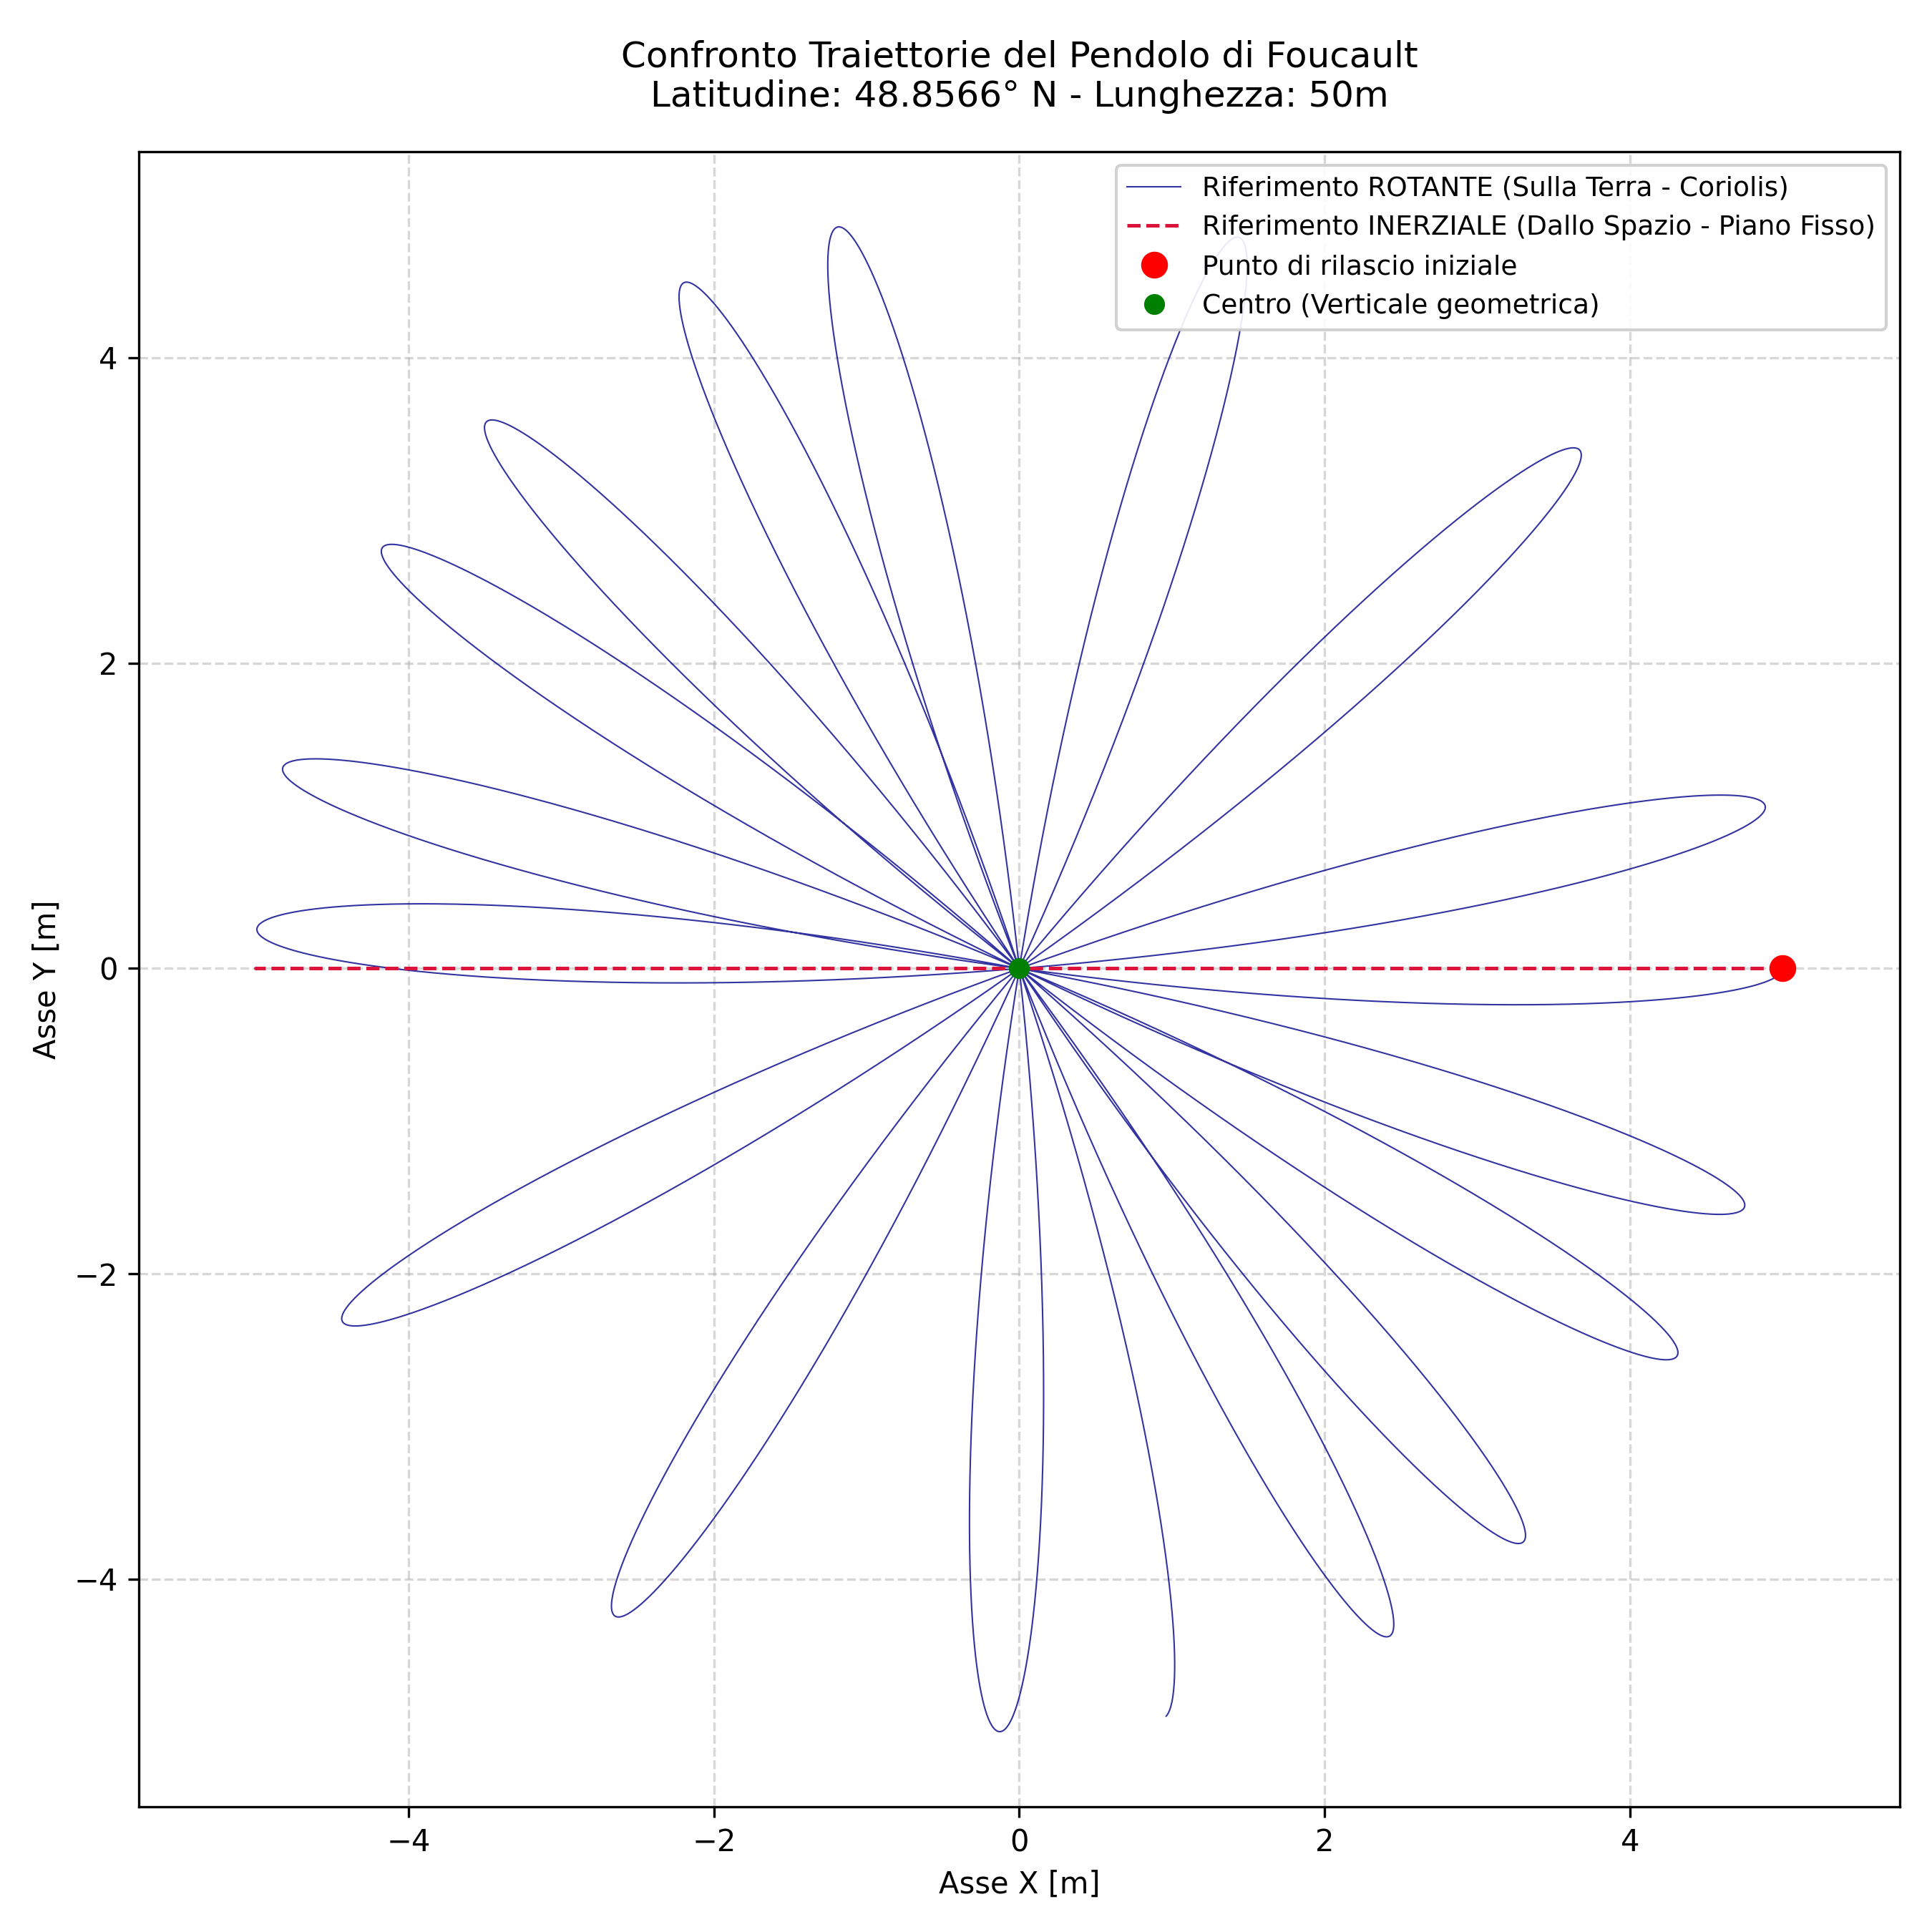
\includegraphics[width=0.6\linewidth]{img/pendoloDiFoucault.png}
    \caption{Traiettoria del pendolo di Foucault nel sistema di riferimento rotante (terrestre) e inerziale (stelle fisse). Si è applicata un'esagerazione voluta della velocità angolare ($\omega = 0.05 \text{ rad/s}$ rispetto a quella reale terrestre $\omega \approx 7.29 \cdot 10^{-5} \text{ rad/s}$) al fine di rendere macroscopicamente apprezzabile il fenomeno della precessione.}
    \label{fig:pendoloDiFoucault}
\end{figure}

\section{Attrito viscoso}
Nei casi in cui le geometrie sono semplici, e il moto è a velocità relativamente basse, allora per calcolare la forza dell'attrito viscoso si può usare la seguente formula:
\begin{equation*}
    \vec{f}_R = -\beta\vec{v}
\end{equation*}
dove:
\begin{itemize}
    \item $\vec{v}$ è la velocità relativa del punto materiale rispetto al fluido
    \item $\beta$ è una costante che dipende dalla geometria del corpo e dalla caratteristiche del fluido, in particolare la sua velocità $\eta$
\end{itemize}
Nel caso in cui il corpo considerato sia sferico, allora vale la legge di Stokes, e implica che:
\begin{equation*}
    \beta = 6\pi\eta R 
\end{equation*}

\newpage

\section{Lavoro ed energia}
Il lavoro di una forza si definisce come la forza applicata ad un punto materiale lungo un certo spostamento, ma il calcolo di quest'ultimo varia in funzione della tipologia di forza considerata:

\begin{itemize}
    \item Forza costante: il lavoro si calcola tramite la formula:
    \begin{equation*}
        L = \vec{f}\cdot \Delta\vec{r}
    \end{equation*}
    \item Forza non costante: nel caso in cui la forza non fosse costante lungo una traiettoria arbitraria, allora per calcolare il lavoro bisogna svolgere l'integrale curvilineo:
    \begin{equation*}
        L = {}_{\gamma}\int_A^B \vec{f}(\vec{r}) d\vec{r}
    \end{equation*}
    Si può definire la forma differenziale del lavoro infinitesimo:
    \[\delta L = \vec{f}d\vec{r}\]
    e anche la forma scalare:
    \begin{align}
        \delta L & = f_xdx + f_ydy + f_zdz \\
        L & = {}_\gamma\int_A^B (f_xdx + f_ydy + f_zdz) \\ 
          & = {}_\gamma\int_A^B f_xdx + {}_\gamma\int_A^B f_ydy + {}_\gamma\int_A^B f_zdz
    \end{align}
\end{itemize}
Il lavoro si misura in Joule ($J$), ed equivale a:
\[1 J = 1Kg \cdot m^{2} \cdot s^{-2}\]

\subsection{Il lavoro totale}
Poiché la risultante delle forze si definisce come:
\[\vec{F} = \sum_i \vec{f}_i\]
allora il lavoro svolto dalla forza risultante è:
\begin{align}
    L & = {}_\gamma\int_A^B \vec{F}\cdot d\vec{r} \\
      & = {}_\gamma\int_A^B \sum_i \vec{f_i}\cdot d\vec{r} \\
      & = \sum_i {}_\gamma\int_A^B \vec{f}_i d\vec{r} \\
      & = \sum_i L_i
\end{align}
Segue quindi che il lavoro totale equivale alla somma dei singoli lavori delle forze.

\subsection{Teorema delle forze vive}
\begin{theorem}
Il teorema delle forze vive (o teorema dell'energia cinetica) stabilisce che il lavoro compiuto dalla forza risultante agente su un punto materiale lungo una data traiettoria è pari alla variazione della sua energia cinetica.
\end{theorem}

\begin{proof}
    Sia $L$ il lavoro svolto dalla forza risultante $\vec{F}$. Per il secondo principio della dinamica vale la relazione:
    \[ \vec{F} = m\vec{a} = m\frac{d\vec{v}}{dt} \]
    Da cui segue che la forma integrale del lavoro, calcolata lungo la curva $\gamma$ tra i punti $A$ e $B$, assume l'espressione:

    \begin{align}
        L & = \int_\gamma m \frac{d\vec{v}}{dt} \cdot d\vec{r}; \quad \quad \vec{v} = \frac{d\vec{r}}{dt} \implies d\vec{r} = \vec{v}dt \\ 
        & = \int_{t_A}^{t_B} m \left( \frac{d\vec{v}}{dt} \cdot \vec{v} \right) dt; \quad \quad \frac{d}{dt}(\vec{v} \cdot \vec{v}) = 2\vec{v} \cdot \frac{d\vec{v}}{dt} \implies \frac{d\vec{v}}{dt} \cdot \vec{v} = \frac{1}{2} \frac{dv^2}{dt} \\
        & = \frac{m}{2} \int_{t_A}^{t_B} \frac{dv^2}{dt}dt \\
        & = \left. \frac{1}{2}mv^2 \right|_{t_A}^{t_B} \\
        & = \frac{1}{2}m v_B^2 - \frac{1}{2}m v_A^2 \\
        & = \Delta K \\
        & = K_B - K_A; \quad \quad K := \frac{1}{2}mv^2 := \text{energia cinetica}
    \end{align}

    La formulazione può essere espressa in forma differenziale considerando uno spostamento infinitesimo $d\vec{r}$ lungo la traiettoria:
    \begin{align}
        \delta L & = \vec{F} \cdot d\vec{r} \\
                & = m \frac{d\vec{v}}{dt} \cdot \vec{v}dt \\ 
                & = \frac{d}{dt}\left(\frac{1}{2}mv^2\right)dt \\
                & = d\left(\frac{1}{2}mv^2\right) \\
                & = dK
    \end{align}
    Integrando entrambi i membri della relazione infinitesima lungo la curva $\gamma$, si ritrova l'equivalenza in forma globale:
    \[ \int_\gamma \delta L = \int_A^B dK \]
\end{proof}

\newpage

\subsection{Forze conservative}
Per una forza conservativa, il lavoro dipende solo dal punto iniziale e finale e non dalla traiettoria, segue quindi che deve valere che:
\[{}_\gamma\int_A^B \vec{f}d\vec{r} = L(A, B) = \int_A^B \vec{f}d\vec{r}\]
Inoltre se la forza è conservativa il lavoro si può esprimere come una differenza di energia potenziale associata alla forza:
\[{}_\gamma\int_A^B \vec{f}d\vec{r} = V(A) - V(B) = -\Delta V; \quad \Delta V = V(B) - V(A)\]
dove quindi $V$ è definita come l'energia potenziale associata alla forza

Si può inoltre definire il lavoro in forma differenziale:
\[\delta L = \vec{f}\cdot d\vec{r} = -dV\]
Nel caso in cui la forza sia conservativa, allora il differenziale è esatto, ovvero $\delta L$ corrisponde al differenziale di una funzione della posizione:

\begin{align}
    \delta L & = \vec{f} \cdot d\vec{r} \\
    & = f_xdx  + f_ydy + f_zdz \\
    & = -dV \\
    & = -(\frac{\partial V}{\partial x} dx + \frac{\partial V}{\partial y} dy + \frac{\partial V}{\partial z} dz) \\ 
    & = -\frac{\partial V}{\partial x} dx - \frac{\partial V}{\partial y} dy - \frac{\partial V}{\partial z} dz 
\end{align}

Allora la forza è conservativa se e solo se vale che:
\[\begin{cases}
        \displaystyle f_x = -\frac{\partial V}{\partial x} \\[1em]
        \displaystyle f_y = -\frac{\partial V}{\partial y} \\[1em]
        \displaystyle f_z = -\frac{\partial V}{\partial z} \\[1em]
    \end{cases}
\]
Definendo l'operatore gradiente, ovvero il vettore delle derivate parziali, come segue:
\[\vec{\nabla}V :=  \frac{\partial V}{\partial x}\hat{\imath} + \frac{\partial V}{\partial y}\hat{\jmath} + \frac{\partial V}{\partial z}\hat{k}\]

allora f è conservativa se:
\[\vec{f} = -\vec{\nabla}V\]

Per verificare la conservatività della forza è anche possibile verificare se l'integrale di circuitazione della forza è pari a 0:
\[\oint \vec{f} d\vec{r} \quad \forall \gamma \text{ chiusa}\]

Esiste inoltre una condizione necessaria per la conservazione, ovvero che il rotore di $f$ sia nullo.
Il rotore si definisce come segue:
\[\vec{\nabla} \times \vec{f} = 
\begin{vmatrix}
\displaystyle \hat{\imath} & \hat{\jmath} & \hat{k} \\
\displaystyle \frac{\partial}{\partial x} & \frac{\partial}{\partial y} & \frac{\partial}{\partial z} \\
\displaystyle f_x & f_y & f_z
\end{vmatrix}
= \left( \frac{\partial f_z}{\partial y} - \frac{\partial f_y}{\partial z} \right) \hat{\imath}  + \left( \frac{\partial f_x}{\partial z} - \frac{\partial f_z}{\partial x} \right) \hat{\jmath}  + \left( \frac{\partial f_y}{\partial x} - \frac{\partial f_x}{\partial y} \right) \hat{k}\]
Segue quindi che affinchè $\vec{\nabla} \times \vec{f} = 0$, deve valere che:
\[\begin{cases}
    \displaystyle \frac{\partial f_x}{\partial y} = \frac{\partial f_y}{\partial x} \\[1em]
    \displaystyle \frac{\partial f_x}{\partial z} = \frac{\partial f_z}{\partial x} \\[1em]
    \displaystyle \frac{\partial f_y}{\partial z} = \frac{\partial f_z}{\partial y} \\[1em]
\end{cases}\]
Per tutti gli spazi semplicemente connessi la condizione è anche sufficiente, mentre ciò non vale per spazi non semplicemente connessi.

Inoltre ogni forza costante è conservativa infatti:
\[L = {}_\gamma \int_A^B \vec{f}d\vec{r} = \vec{f} {}_\gamma \int_A^B d\vec{r} = \vec{f}(\vec{r}_B - \vec{r}_A) = \vec{f}\Delta\vec{r}\]



\subsubsection{Esempi}
Se si ha una forza conservativa + altre forze generiche, in cui si ha $\Delta K = 0$, allora:
\[L_{tot} = -\Delta V \Longrightarrow L_{altre}\]

\subsection{Conservazione dell' energia meccanica}
Se sul punto materiale agiscono più forze conservative, per il teorema delle forze vive, si ha che:
\[dK = \delta L_{tot} = \sum_i \delta L_i\]
Inoltre vale che:
\[\delta L_i = -dV_i\]
Si può quindi definire una energia potenziale totale:
\[V = \sum_i V_i\]
allora:
\[dK = \sum_i -dV_i = -dV\]
segue che:
\[d(K + V) = 0\]
Definendo l'energia meccanica come la somma tra l'energia cinetica e l'energia potenziale totale, si ha che l'energia meccanica del punto materiale si conserva:
\[E_M := K + V\]
Infatti poiché:
\[dE_M = 0 \iff E_M \text{ è costante}\]

\subsubsection{Esempio}
Se un un corpo agiscono sia forze conservative, sia forze non conservative, si ha che:
\[dK = \delta L = \delta L^{nc} + \delta L^{c} = \delta L^{nc} - dV\]
\[\Rightarrow d(K + V) = dE_M = \delta L^{nc} \iff \Delta E_M = \delta L^{nc}\]


\section{Moti unidimensionali}
Si consideri un moto lungo una traiettoria prestabilita, come ad esempio:
\begin{itemize}
    \item moto verticale di un punto soggetto alla forza peso
    \item moto di un punto soggetto a un vincolo bilaterale
\end{itemize}
Metodi di soluzione:
\begin{itemize}
    \item Proiezione della seconda legge di Newton lungo la direzione tangente alla traiettoria
    \item In presenza di forze conservative si può applicare la legge della conservazione dell'energia meccanica:
    
    Si definisce la coordinata curvilinea $s$ lungo la traiettoria, allora si ha una energia potenziale totale in funzione della posizione:
    \[V(\vec{r}) \Rightarrow V(\vec{r}(s))\]
    Allora poiché agiscono solo forze conservative, la differenza di energia meccanica è nulla:
    \begin{align}
        \Delta E_M & = 0 \\ 
        K + V & = \text{costante} \\
        \frac{1}{2}m\dot{s}^2 + V(s) & = \text{costante} \\
    \end{align}
    Derivando rispetto al tempo si ottiene:
    \[m\dot{s}\ddot{s} + \frac{dV}{ds}\dot{s} = 0\]
    ed è verificata se:
    \[\dot{s} = 0 \vee m\ddot{s} = -\frac{dV}{ds}\]
    il secondo membro è il II principio proiettato, segue che:
    \begin{align}
        -\frac{dV}{ds} = -\sum_i \frac{\partial V}{dx_i} \frac{dx_i}{ds} = -\vec{\nabla}V \frac{d\vec{r}}{ds} = \vec{f} \frac{d\vec{r}}{ds} = \vec{f} \hat{u}_t = f_{traiettoria}
    \end{align}
    segue che:
    \[m\ddot{s} = f\]
    Nell'applicazione di questo metodo in funzione della variabile rispetto alla quale si deriva l'energia potenziale si può trovare una forza o un momento, in fatti si può parlare di variabili generalizzate, attraverso le quali derivando l'energia potenziale si trova la causa della loro variazione, nel caso di una variabile lineare come $(x, y, z, ...)$ si otterrà una forza, nel caso di $(\theta, \varphi, ...)$ un momento.
\end{itemize}
I due metodi sono equivalenti nel caso di moti unidimensionali e con forze conservative (o forze non conservative che svolgono lavoro nullo).

\newpage

\subsection{Conservazione dell'energia negli oscillatori armonici}
Come già visto un oscillatore armonico è descritto dell'equazione differenziale:
\[\ddot{x} + \omega_0^2x = 0; \quad \quad w_0 = \sqrt{\frac{k}{m}}\]
e la soluzione generale è:
\[x(t) = A\cos(w_0t + \theta_0)\]
dalla legge oraria si può ricavare immediatamente $K$ e $V$ in funzione del tempo, infatti:
\begin{align}
    V(t) & = \frac{1}{2}kx^2(t) = \frac{1}{2}kA^2\cos^2(\omega_0t + \theta_0) \\
    K(t) & = \frac{1}{2}mv^2 \\
    & = \frac{1}{2}m\omega_0^2A^2\sin^2(\omega_0t + \theta_0) \\
    & = \frac{1}{2}kA^2\sin^2(\omega_0t + \theta_0)
\end{align}
\[\Rightarrow E_M = V(t) + K(t) = \frac{1}{2}kA^2 = \text{costante}\]

L'energia potenziale massima si ha quando nel punto corrispondente alla massima estensione della molla $A$, dove l'energia cinetica è nulla.

Invece l'energia cinetica è massima quando $x=0$, quindi quando la molla non esercita forze sul corpo.

I valori medi di $K$ e $V$ in un certo periodo sono uguali, ed equivale a:
\[<V> = \frac{1}{2}k\frac{A^2}{T} \int_0^T \cos^2(\omega_0t + \theta_0)dt \frac{1}{4}kA^2 = \frac{1}{4} m\omega_0^2A^2 = <K>\]

\paragraph{Piccole oscillazioni del pendolo semplice}
Come già noto, nel limite delle piccole oscillazioni, il pendono ideale soddisfa l'equazione:
\begin{equation}
    \dv[2]{\theta}{t} + \omega_0^2 \theta = 0; \quad \omega_0^2 = \frac{g}{L}
\end{equation}
o, equivalentemente definendo $s = \theta L$, soddisfa:
\begin{equation}
    \dv[2]{s}{t} + \omega_0^2 s = 0; \quad \omega_0^2 = \frac{g}{L}
\end{equation}
Risolvendo l'equazione differenziale e imponendo le condizioni iniziali, si deriva la legge orario:
\begin{equation}
    s(t) = S_0 \cos(\omega_0 t + \theta_0)
\end{equation}
dalla quale è possibile calcolare l'energia cinetica:
\begin{align}
    K & = \frac{1}{2}m\dot{s}^2 \\
      & = \frac{1}{2}m S_0^2 \omega_0^2 \sin^2(\omega_0 t + \theta_0)
\end{align}
È possible calcolare l'energia potenziale associata alla forza peso, scegliendo come punto $z = 0$ la quota del pendolo quando $\theta = 0$, ottenendo:
\begin{align}
    V(s) & = mgz(s) \\
         & = mgL(1 - \cos(\frac{s}{L}))
\end{align}
\newpage

\subsection{Equilibrio ed energia potenziale}
Si consideri un punto materiale soggetto a un certo numero di forze, allora si definisce punto di equilibrio un punto in cui il corpo resta in quiete se è inizialmente in quiete, la condizione necessaria e sufficiente affinché ciò avvenga è che la risultante $\vec{f}$ delle forze che agiscono sul corpo sia nulla.

Se si suppone che le forze in gioco siano tutte conservative, allora anche $\vec{f}$ è conservativa, allora vale che:
\[\vec{f} = -\vec{\nabla}V\]
pertanto la condizione di equilibrio si traduce nelle seguenti equazioni:
\[\frac{\partial V}{\partial x} = 0; \quad \quad \frac{\partial V}{\partial y} = 0; \quad \quad \frac{\partial V}{\partial z} = 0\]

Ciò significa quindi che un punto di equilibrio corrisponde ad un massimo relativo, un minimo relativo o punto di sella.

Il comportamento di un punto materiale in presenza di \textit{piccoli spostamenti} dal punto di equilibrio (dovuto ad una perturbazione esterna non inclusa in $\vec{f}$) è molto diverso nei 3 casi, infatti:
\begin{itemize}
    \item \textbf{minimo relativo}: la forza $f$ si comporta come una forza di richiamo (essendo $\vec{f} = -\vec{\nabla}V$) e quindi tende a riportare il corpo verso una posizione di equilibrio (in realtà oscilla intorno alla posizione), pertanto si definisce quindi equilibrio stabile.

    \item \textbf{massimo relativo}: il corpo tende ad allontanarsi dal punto di equilibrio, pertanto si definisce equilibrio instabile.

    \item \textbf{punto di sella}: il corpo si comporta in modo diverso in base alla direzione della forza perturbatrice, se esse è lungo alcune direzioni il corpo tende ad allontanarsi e quindi si definisce equilibrio instabile.
\end{itemize}
Invece se $\vec{f}$ è costante in un intorno del punto di equilibrio esso è detto punto di equilibrio indifferente

%TO DO INSERIRE DA PAGINE 18 IN POI LEZIONE 19

\subsection{Potenza}
La potenza media si definisce come il rapporto tra il lavoro e il tempo impiegato, come segue:
\[P_m = \frac{\Delta L}{\Delta t}\]
Attraverso il procedimento di limite, si ottiene la potenza istantanea, che equivale a:
\[P = \lim_{\Delta t \to 0} \frac{\Delta L}{\Delta t} = \frac{\partial L}{dt}\]
Nel caso del lavoro compiuto su un punto materiale, vale che:
\[P = \frac{\partial L}{dt} = \vec{f} \cdot \frac{d\vec{r}}{dt} = \vec{f} \cdot \vec{v}\]
La potenza si misura in:
\begin{itemize}
    \item Watt, ove:
    \[1 W = 1Js^{-1} = 1Kgm^2s^{-3}\]

    \item Cavallo vapore, ove:
    \[1hp = 735.5 W\]

    \item Chilo Wattora, ove:
    \[1KWh= 1 KW \cdot 3600 s = 3.6 \cdot 10^{6}J\]
\end{itemize}

\section{Moto oscillatorio smorzato}
Si consideri il moto di una massa m, collegata ad una molla con lunghezza a riposo nulla, lungo un piano senza attrito, il moto avviene in un mezzo che provoca attrito viscoso, allora per il secondo principio di Newton:

\begin{align}
    m\ddot{x} & = -kx - \beta \dot x \\
    m\ddot{x} + kx + \beta \dot x & = 0; \quad \quad x(t) = e^{\lambda t}
\end{align}
\begin{equation*}
     \\
    (m\lambda^2 + \beta \lambda + k)e^{\lambda t} = 0 \iff \lambda_{1, 2} = \frac{-\beta \pm \sqrt{\beta^2 - 4mk}}{2m}
\end{equation*}
La tipologia di moto dipende dal segno del determinante, infatti se:
\begin{itemize}
    \item $\beta^2 - 4mk > 0$, si avrà un moto oscillatorio sovra-smorzato
    \item $\beta^2 - 4mk = 0$, si avrà un moto oscillatorio criticamente smorzato
    \item $\beta^2 - 4mk < 0$, si avrà un moto oscillatorio sotto-smorzato
\end{itemize}

\newpage

\subsection{Moto oscillatorio sovra-smorzato}
Si ha:
\[\lambda_{1, 2} = \frac{-\beta \pm \sqrt{\beta^2 - 4mk}}{2m}\]
e quindi:
\[x(t) = C_1e^{\lambda_1 t} + C_2e^{\lambda_2 t}\]
La massa può passare al più una volta per la posizione di equilibrio. Questo comportamento dipende strettamente dalle condizioni iniziali di posizione $x_0$ e velocità $v_0$. Ecco le tre casistiche principali:

\begin{figure}[h]
    \centering
    \begin{minipage}{0.48\textwidth}
        \centering
        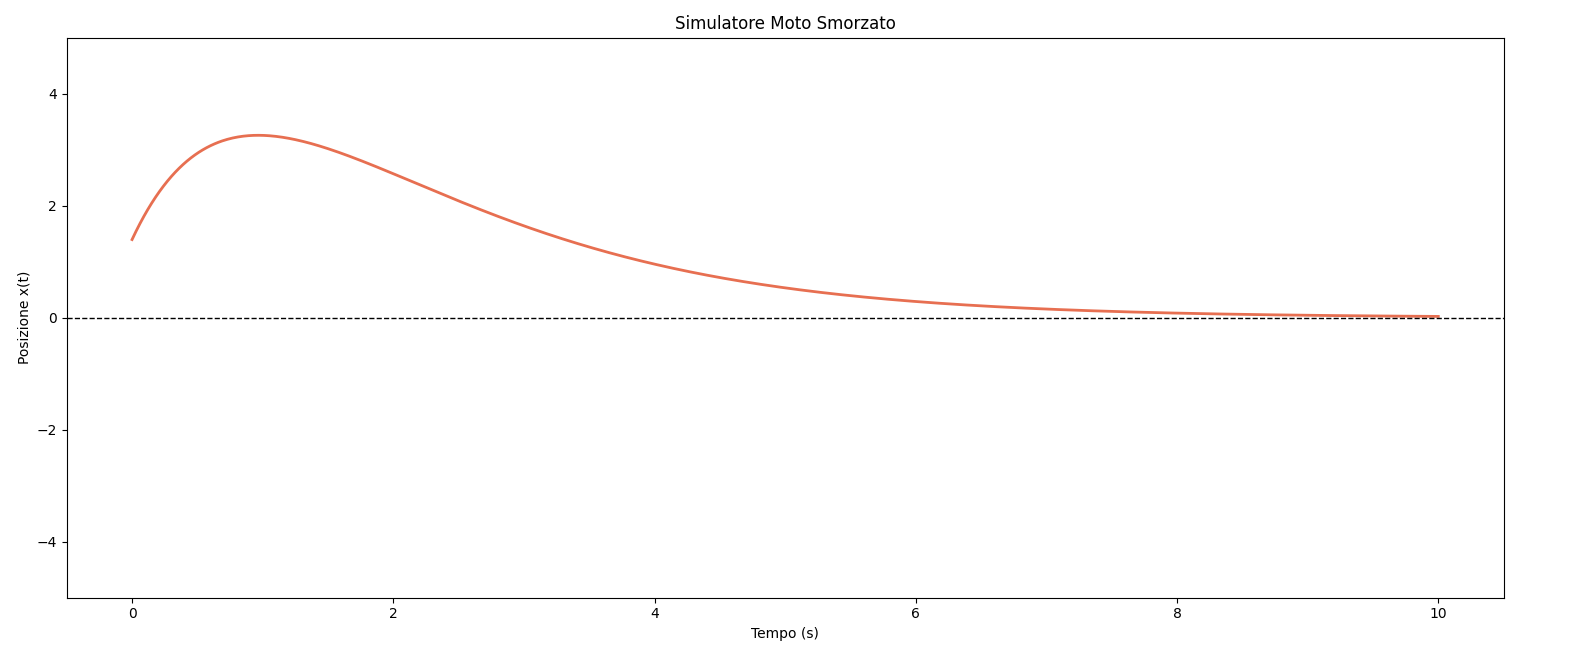
\includegraphics[width=\linewidth]{dotx_pos_grande in modulo.png}
        \caption{Velocità iniziale positiva e grande in modulo.}
    \end{minipage}
    \hfill
    \begin{minipage}{0.48\textwidth}
        \centering
        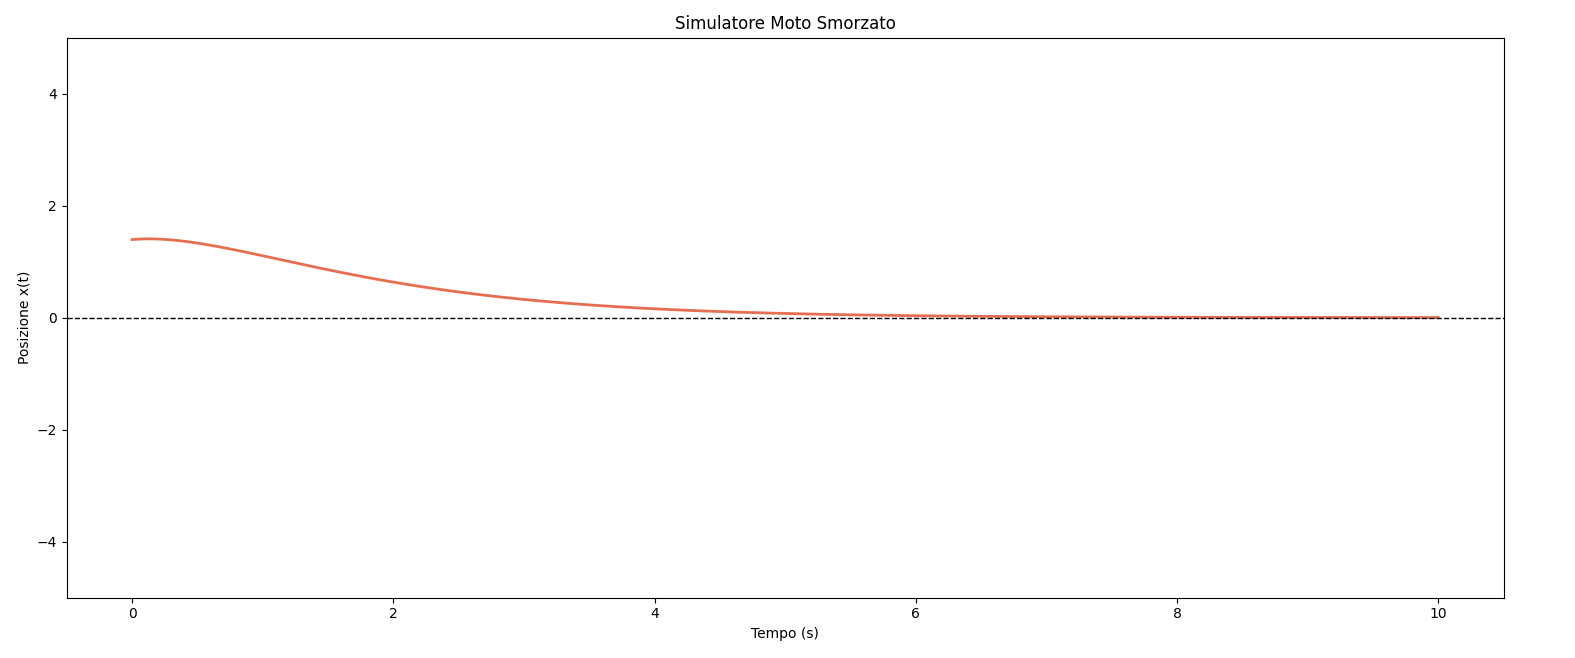
\includegraphics[width=\linewidth]{dotx_pos_piccola in modulo.png}
        \caption{Velocità iniziale positiva ma piccola in modulo.}
    \end{minipage}

    \vspace{1cm}

    \begin{minipage}{0.48\textwidth}
        \centering
        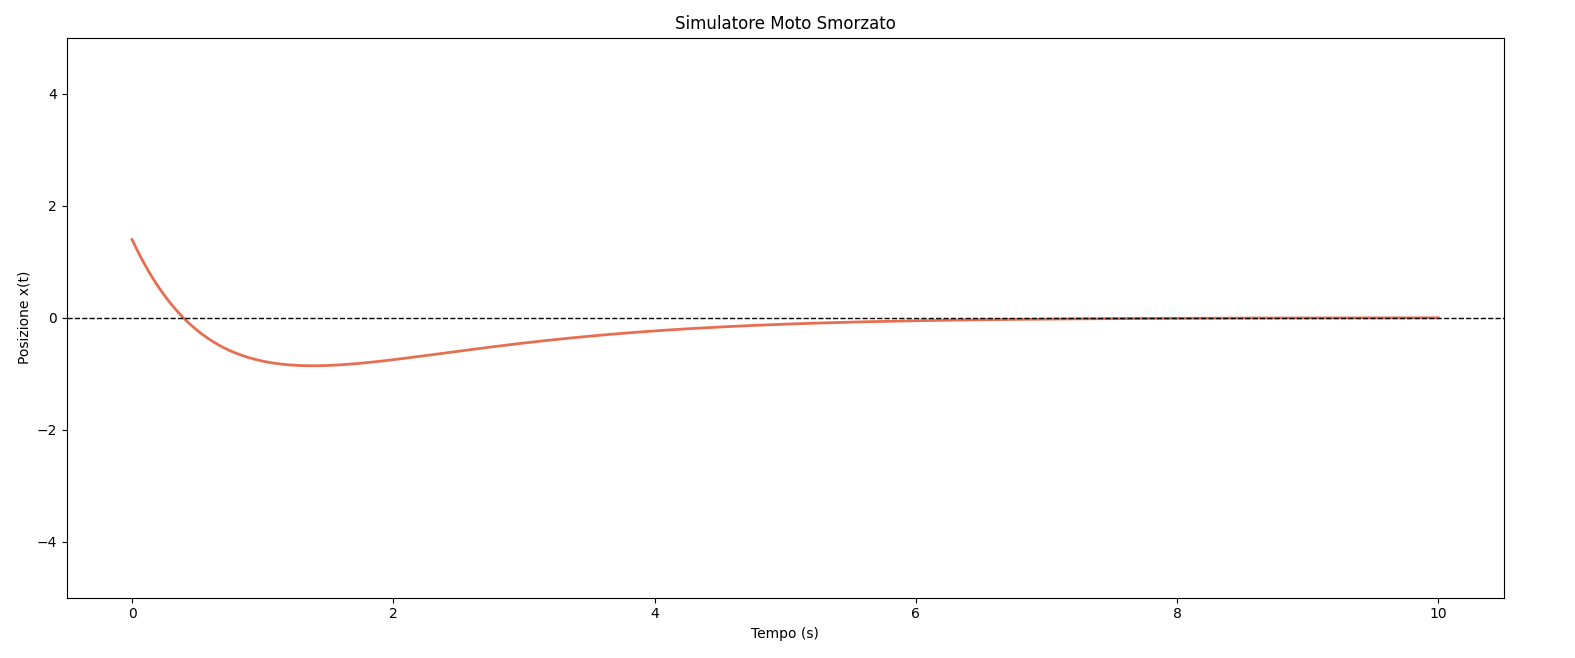
\includegraphics[width=\linewidth]{dotx_neg_grande in modulo.png}
        \caption{Velocità iniziale negativa e grande in modulo.}
    \end{minipage}
\end{figure}

\newpage

\subsection{Moto oscillatorio criticamente smorzato}
Si ha la condizione $\beta^2 - 4mk = 0$, pertanto le radici sono reali e coincidenti:
\[\lambda_1 = \lambda_2 = -\lambda = -\frac{\beta}{2m}\]
La soluzione generale assume la forma:
\[x(t) = (C_1 + C_2 t)e^{-\lambda t}\]
Il sistema anche in questo caso passa al più una volta nel punto di equilibrio $x = 0$, e ciò succede se e solo se:
\[\exists t^* \quad | \quad C_1 + C_2t^* = 0 \iff t^* = -\frac{C_1}{C_2} \iff C_1C_2<0\]
Le costanti $C_1$ e $C_2$ si determinano imponendo le condizioni iniziali $x(0) = x_0$ e $\dot{x}(0) = \dot{x}_0$:
\begin{itemize}
    \item $C_1 = x_0$
    \item $C_2 = \dot{x}_0 + \lambda x_0$
\end{itemize}

Ma deve essere verificata la condizione $C_1C_2<0$, quindi se:
\begin{align}
    x_0 > 0 \implies \dot{x}_0 & < \frac{\beta}{2m}x_0 \\
    x_0 < 0 \implies \dot{x}_0 & > \frac{\beta}{2m}x_0
\end{align}
\[\implies C_1C_2 < 0 \iff x_0\dot{x}_0 < 0 \iff |x_0| > \frac{\beta}{2m}|\dot{x}_0|\]

Di seguito le tre casistiche principali basate sul valore della velocità iniziale $v_0$:

\begin{figure}[h]
    \centering
    \begin{minipage}{0.48\textwidth}
        \centering
        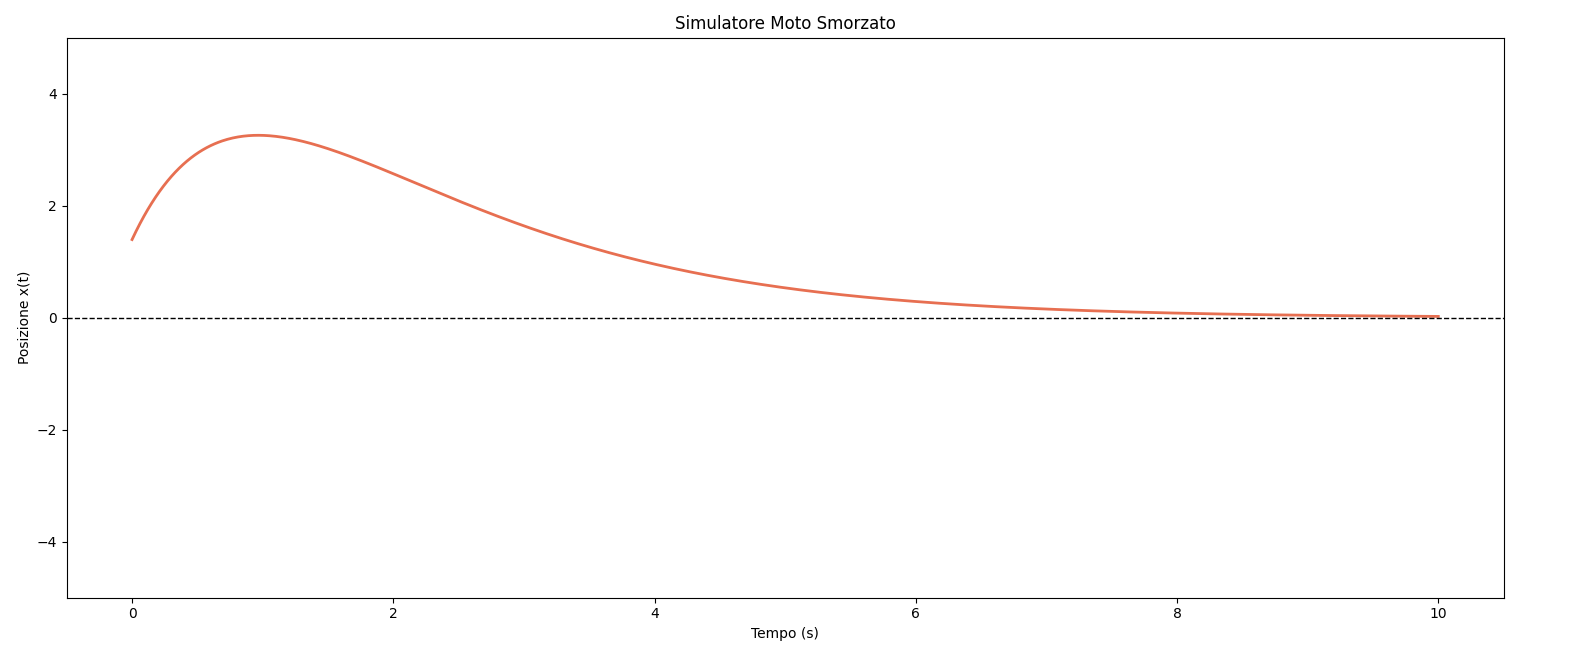
\includegraphics[width=\linewidth]{dotx_pos_grande in modulo.png}
        \caption{Velocità iniziale positiva e grande in modulo e $C_1C_2 > 0$.}
    \end{minipage}
    \hfill
    \begin{minipage}{0.48\textwidth}
        \centering
        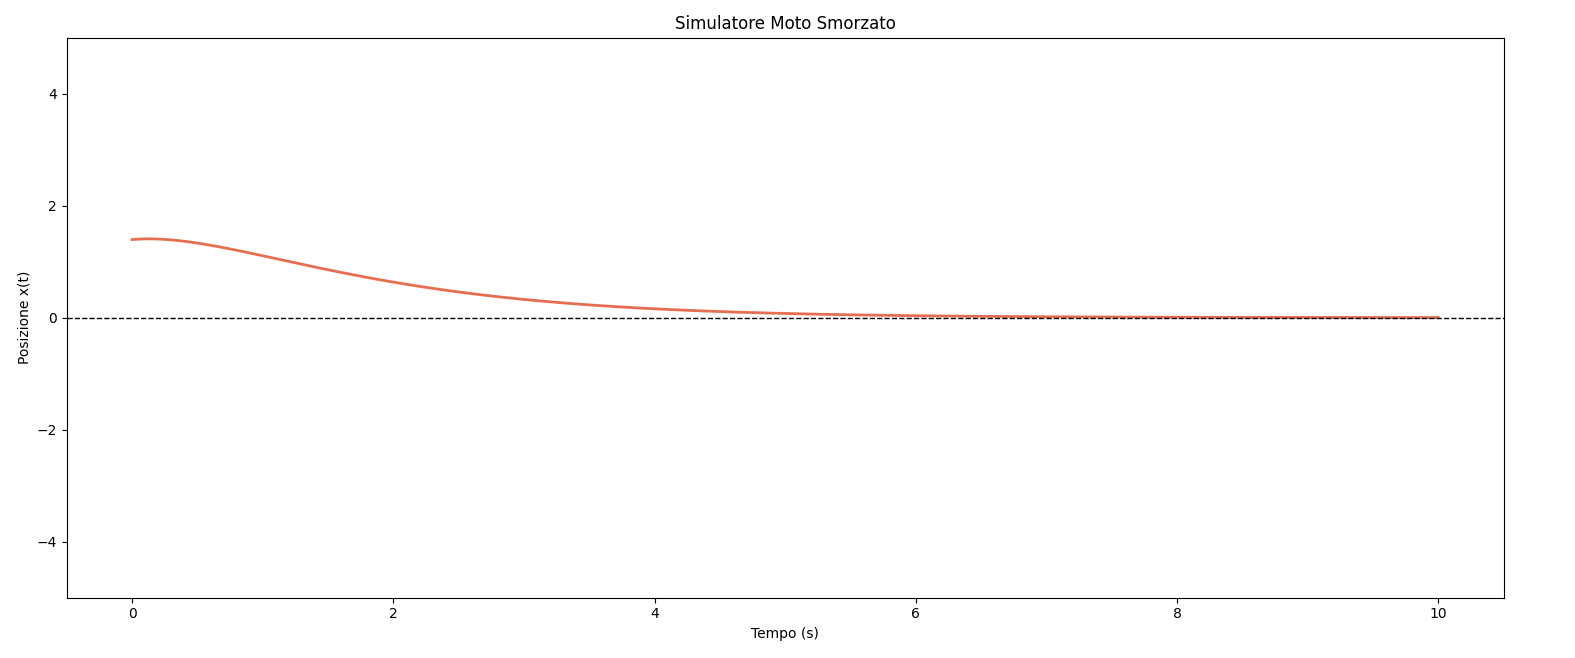
\includegraphics[width=\linewidth]{dotx_pos_piccola in modulo.png}
        \caption{Velocità iniziale positiva ma piccola in modulo e $C_1C_2 > 0$.}
    \end{minipage}

    \vspace{1cm}

    \begin{minipage}{0.48\textwidth}
        \centering
        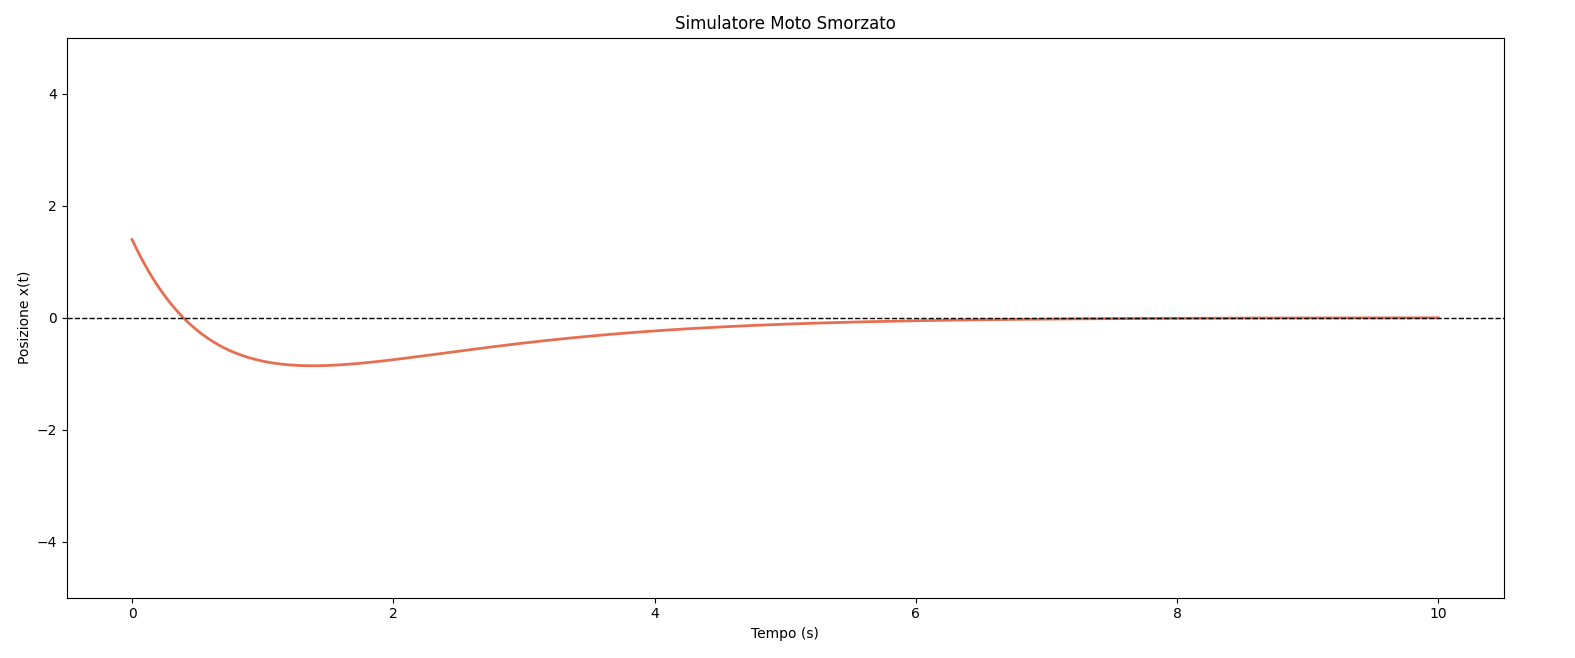
\includegraphics[width=\linewidth]{dotx_neg_grande in modulo.png}
        \caption{Velocità iniziale negativa e grande in modulo e $C_1C_2 < 0$.}
    \end{minipage}
\end{figure}

\newpage

\subsection{Moto oscillatorio sotto-smorzato}
Si ha la condizione $\beta^2 - 4mk < 0$, pertanto ci sono due soluzioni complesse coniugate:
\begin{align}
    \lambda_{1,2} & = \frac{- \beta \pm i \sqrt{4mk - \beta^2}}{2m} \\
    & = -\frac{\beta}{2m} \pm i \sqrt{\frac{k}{m} - \frac{\beta^2}{4m^2}}; \quad \omega_0^2 = \frac{k}{m} \\
    & = -\frac{\beta}{2m} \pm i \sqrt{\omega_0^2 - \frac{\beta^2}{4m^2}}; \quad \omega_1^2 = \sqrt{\omega_0^2 - \frac{\beta^2}{4m^2}} \\
    & = -\frac{\beta}{2m} \pm i \omega_1
\end{align}
allora la soluzione è:
\[x(t) = e^{-\frac{\beta}{2m}t} \left(Ae^{i\omega_1t} + Be^{-i\omega_1t}\right)\]
sapendo che:
\[e^{\pm i \omega_1t} = \cos(\omega_1t) \pm i\sin(\omega_1t)\]
allora:
\[x(t) = e^{-\frac{\beta}{2m}t} \left((A + B)\cos(\omega_1t) + i(A - B)\sin(\omega_1t)\right)\]
ove:
\[x(t) \in \mathbb{R} \iff A = \overline{B}\]
quindi si hanno soluzioni reali e se soltanto se A e B sono complessi coniugati, allora segue che la soluzione è:
\begin{align}
    x(t) & = e^{-\frac{\beta}{2m}t}(\alpha\cos(\omega_1t) + \gamma\sin(\omega_1t)) \\
         & = e^{-\frac{\beta}{2m}t}(C_1\cos(\omega_1t + C_2)) 
\end{align}
La casistica principale di questo tipo di moto è:

\begin{figure}[h]
    \centering
    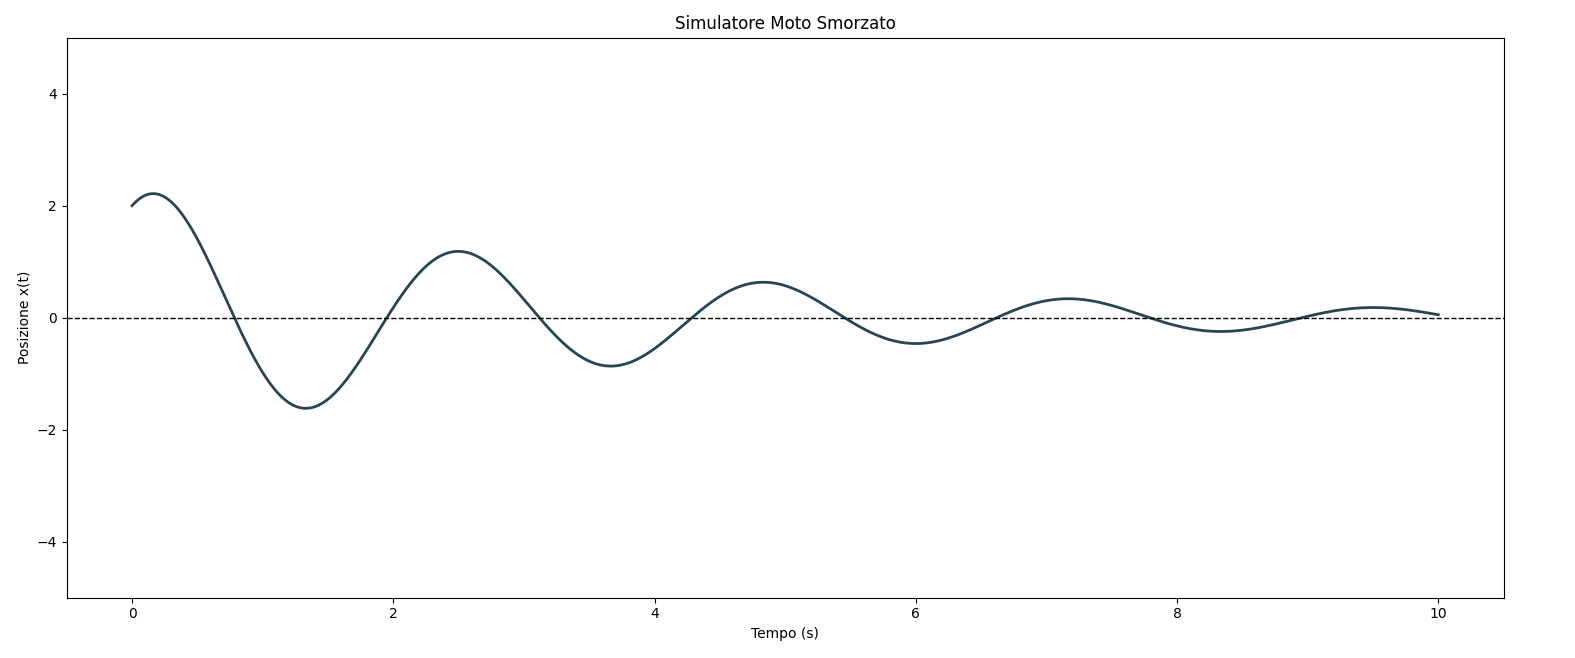
\includegraphics[width=0.5\linewidth]{sottoSmorzato.png}
    \caption{Velocità iniziale positiva}
    \label{fig:placeholder}
\end{figure}

\newpage

\section{Moto oscillatorio forzato}
Se ad un oscillatore soggetto ad attrito viscoso si applica una forza eccitante sinusoidale, si ottiene un'equazione differenziale del secondo ordine non omogenea:
\[m\ddot{x} + \beta\dot{x} + kx = F\cos(\omega t)\]
nella quale $\omega$ è in generale diversa dalla frequenza propria del sistema $\omega_0 = \sqrt{\frac{k}{m}}$. 
Per risolvere conviene renderla una equazione differenziale complessa, che paradossalmente si risolve più semplicemente, infatti:
\[m\ddot{x} + \beta\dot{x} + kx = Fe^{i\omega t}\]
assumendo che:
\[\tilde{x}(t) = Ae^{i\omega t}, \quad A \in \mathbb{C}\]
derivando e inserendo dell'equazione differenziale, si ottiene:
\[-m\omega^2Ae^{i\omega t} + \beta i \omega Ae^{i\omega t} + kAe^{i\omega t} = Fe^{i\omega t}\]
segue che:
\[A((k - m\omega^2) + i\beta\omega) = F\]
\[A = \frac{F}{Z}; \quad \quad Z := (k - m\omega^2) + i\beta\omega:= \text{impedenza}\]
L'impedenza è un numero complesso dove:
\[\begin{cases}
    Z = |Z|e^{i\varphi} \\
    |Z| = \sqrt{(k - m\omega^2)^2 + (\beta\omega)^2} \\
    \varphi = \arctan(\frac{\beta\omega}{k - m\omega^2})
\end{cases}\]
allora:
\[A = \frac{F}{|Z|}e^{-i\varphi}\]
segue che:
\[\tilde{x}(t) = \frac{F}{\sqrt{(k - m\omega^2)^2 + (\beta\omega)^2}}e^{i(\omega t - \varphi)}\]
se si considera solo la parte reale di $\tilde{x}(t)$, si ottiene:

\begin{align}
    x(t) & = \frac{F}{\sqrt{(k - m\omega^2)^2 + (\beta\omega)^2}}\cos(\omega t - \varphi) \\
         & = \frac{F}{m\sqrt{(\omega_0^2 - \omega^2)^2 + (\frac{\beta\omega}{m})^2}}\cos(\omega t - \varphi) \\
         & = \frac{F}{m\sqrt{(\omega_0^2 - \omega^2)^2 + (\frac{\beta\omega}{m})^2}}\cos(\omega t - \arctan(\frac{\beta\omega}{k - m\omega^2}))
\end{align}

La soluzione trovata è quella particolare, detta anche soluzione del regime stazionario, infatti la soluzione completa deriva dalla somma di questa soluzione con quella dell'equazione differenziale omogenea, quindi senza la forza eccitante, che viene detta anche transitoria, in quanto per $t >> \tau$ la soluzione omogenea tende a 0, quindi per tempi molto maggiori del tempo caratteristico l'unica soluzione che in buona approssimazione descrive il sistema è quella stazionaria appena trovata.

Inoltre quando $\beta$ è molto piccolo $(\beta \to 0)$ la funzione ha un massimo per $\omega \to \omega_0$, infatti:

\begin{figure}[h]
    \centering
    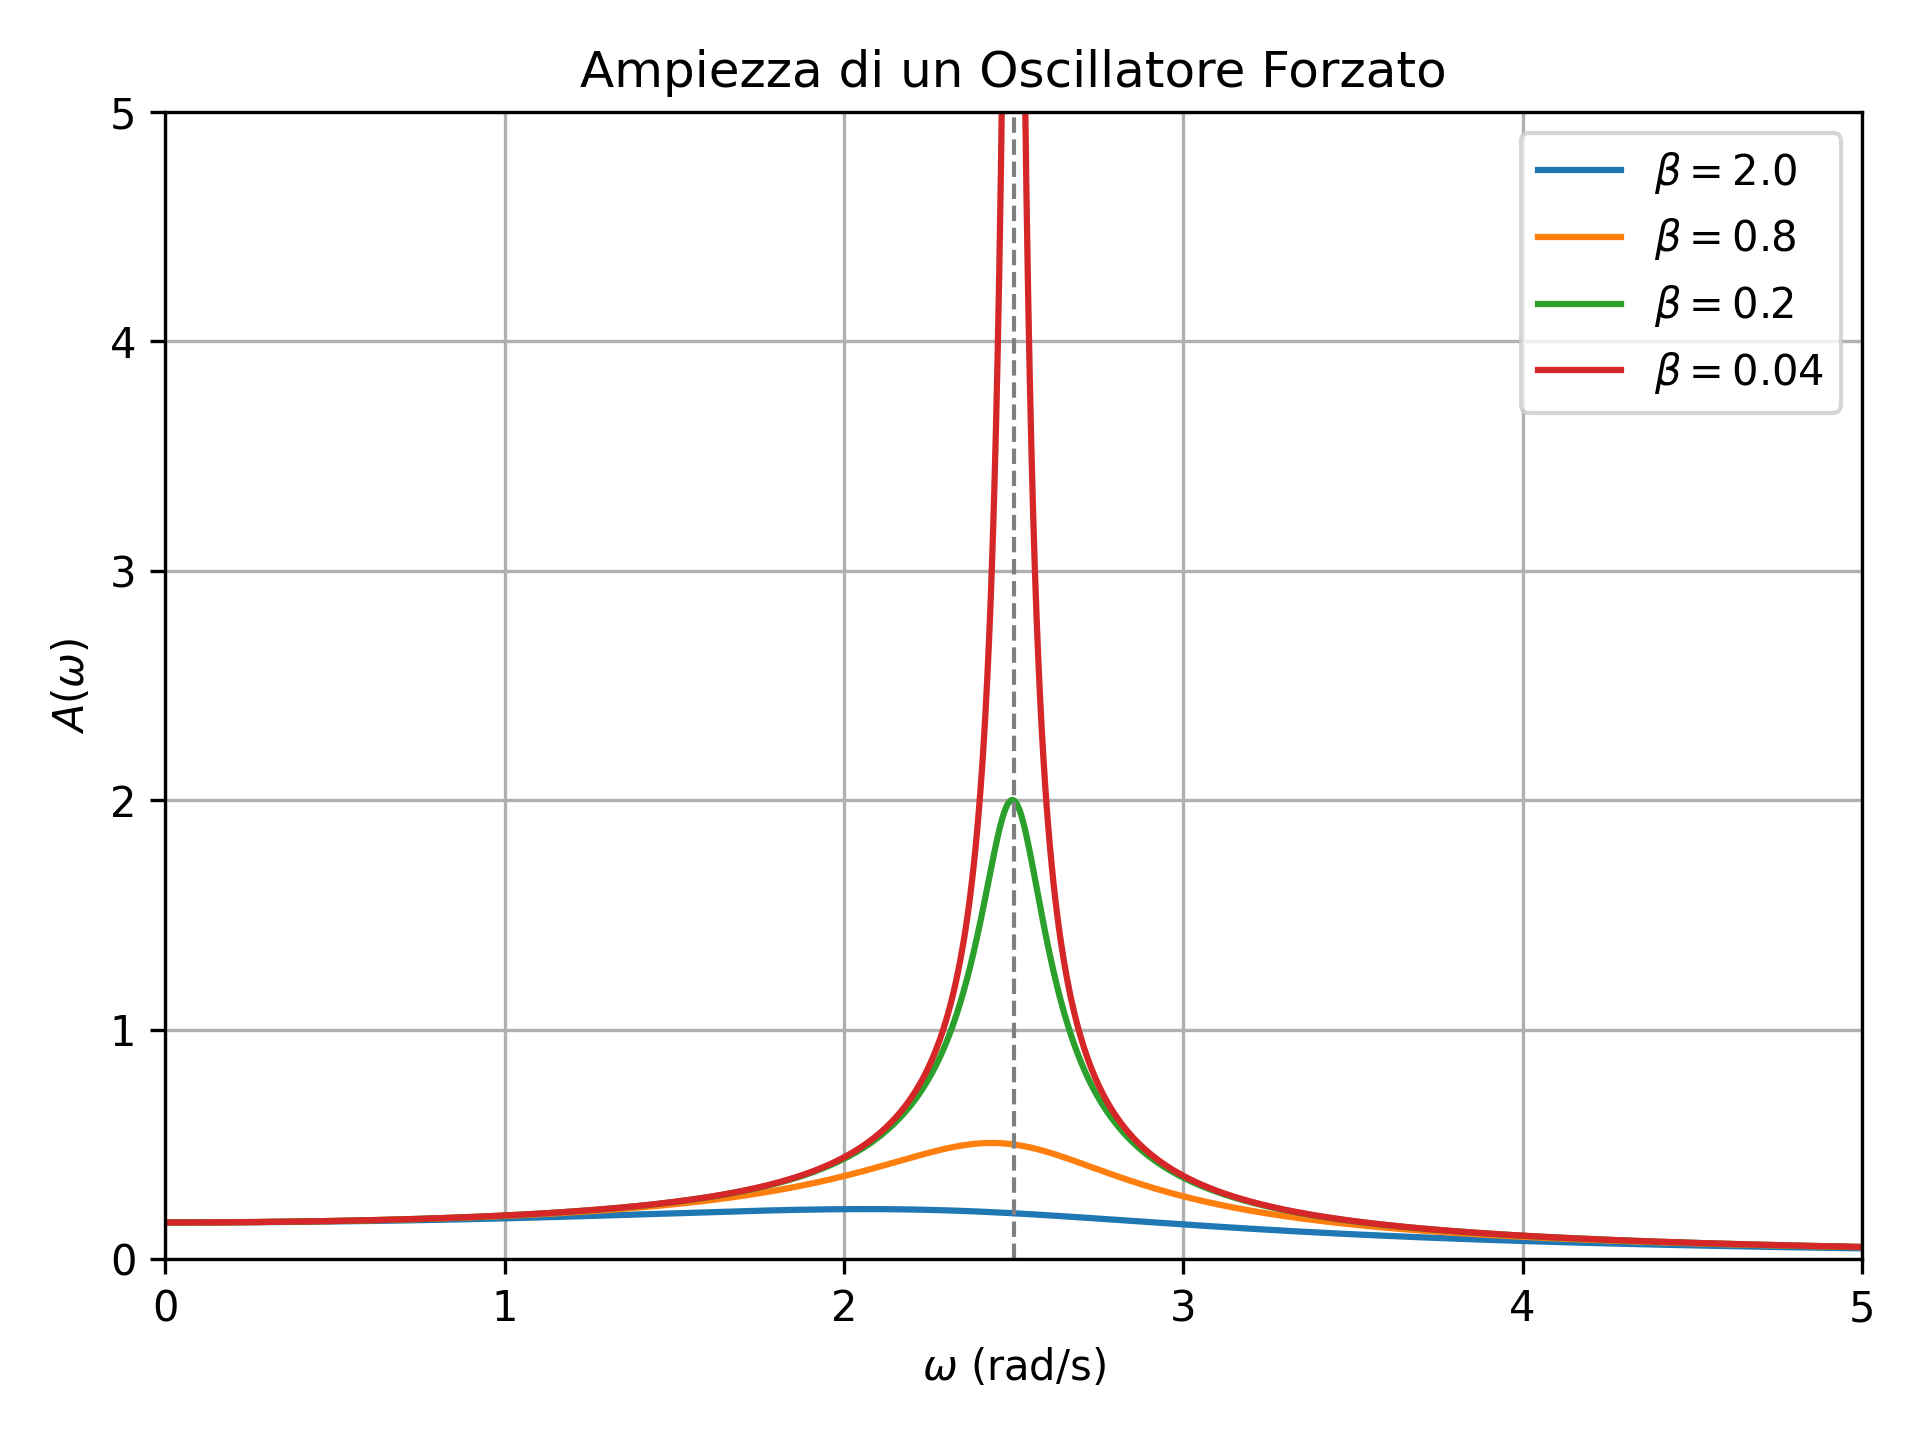
\includegraphics[width=0.75\linewidth]{oscillatore_forzato.png}
    \caption{Grafico dell'ampiezza in funzione di omega in cui $\beta \to 0$ }
    \label{fig:oscillatoreForzato}
\end{figure}

In presenza di un termine forzante generico e non sinusoidale, è possibile ricorrere allo sviluppo in Serie di Fourier per decomporre la funzione in una somma di componenti armoniche. Questo approccio permette di esprimere una sollecitazione periodica complessa come una combinazione di seni e coseni a frequenze discrete (multiple della fondamentale $\omega_0$). Grazie al Principio di Sovrapposizione, la risposta del sistema può essere quindi calcolata come la somma delle risposte individuali dell'oscillatore a ciascuna di queste componenti.

\newpage

\section{Oscillatori accoppiati}
Se si considera un sistema di N masse collegate tramite $N + 1$ molle, con le opportune definizioni di $x_i$ in modo che sia il centro della massa i-esima, allora si ottiene un sistema del tipo:
\[\begin{cases}
    m\ddot{x}_1 = -k_1x_1 + k_2(x_2 - x_1) \\
    m\ddot{x}_2 = -k_1x_2 - k_2(x_2 - x_1) \\
\end{cases} \implies 
\begin{cases}
    m\ddot{x}_1 = -(k_1 + k_2)x_1 + k_2x_2 \\
    m\ddot{x}_2 = k_2x_1 -(k_1 + k_2)x_2  \\
\end{cases}\]
definendo:
\[\omega_0 := \sqrt{\frac{k_2}{m}}, \quad c := \frac{k1 + k2}{m}\]
si ottiene:
\[\begin{cases}
    \ddot{x}_1 = -cx_1 + \omega_0^2x_2 \\
    \ddot{x}_2 = \omega_0^2x_1 -cx_2   \\
\end{cases}\]
Assumendo una soluzione del tipo:
\[x_i (t) = X_i\cos(\Omega t +\Phi)\]
si ottiene:
\[\begin{cases}
    -\Omega^2A\cos(\Omega t +\Phi) = -cA\cos(\Omega t +\Phi) + \omega_0^2B\cos(\Omega t +\Phi) \\
    -\Omega^2B\cos(\Omega t +\Phi) = \omega_0^2A\cos(\Omega t +\Phi) -cB\cos(\Omega t +\Phi)   \\
\end{cases} \implies \begin{cases}
    (\Omega^2 - c\omega_0^2)A + \omega_0^2B = 0 \\
    \omega_0^2A + (\Omega^2 - c\omega_0^2)B = 0  \\
\end{cases}
\]

Il sistema ha soluzioni non banali se la matrice dai coefficienti ha determinante nullo, quindi se:

\[\begin{vmatrix}
    \Omega^2 - c\omega_0^2 & \omega_0^2\\
    \omega_0^2& \Omega^2 - c\omega_0^2
\end{vmatrix} = 0 \iff \]
\[\iff (\Omega^2 - c\omega_0^2)^2 - \omega_0^4 = 0 \iff \Omega^2 - c\omega_0^2 = \pm \omega_0^2 \implies \begin{cases}
    \Omega_1 = \omega_0\sqrt{c - 1} \\
    \Omega_2 = \omega_0\sqrt{c + 1}
\end{cases}\]

Moltiplicando la matrice precedentemente trovata, e sostituendo al posto di $\Omega$ l'autovalore trovato dal polinomio caratteristico, si ottiene l'autovettore che spiega il moto delle due masse, quindi le due soluzioni trovate sono dette modi normali, mentre la soluzione generale deriva dalla somma dei due modi normali, come segue:

\[x_1(t) = A\cos(\Omega_1 t + \Phi_1) + B\cos(\Omega_2 t + \Phi_2) \]
\[x_2(t) = A\cos(\Omega_1 t + \Phi_1) - B\cos(\Omega_2 t + \Phi_2) \]

\newpage

\chapter{Dinamica dei sistemi}

\section{Definizioni preliminare per sistemi discreti}

\subsection{Centro di massa}
Nei sistemi discreti, composti da un numero finito n di punti materiali ciascuno con massa $m_i$ e posizione $r_i$. 

Il centro di massa $r_c$ si definisce come la media pesata delle posizioni dei singoli punti materiali rispetto alle loro masse:

\begin{equation}
    r_c = \frac{\sum_i m_i\vec{r}_i}{\sum_i m_i}
\end{equation}

\subsection{Proprietà distributiva}
Per un sistema con un numero n di corpo si possono considerare N sotto sistemi, ove $N < n$, infatti ad esempio è possibile calcolare il centro di massa del sistema totale nel seguente modo:
\begin{equation}
    \vec{r}_c = \frac{\sum_i M_i\vec{r}_{c_i}}{\sum_i M_i}
\end{equation}

\subsection{Asse di simmetria}
Un sistema possiede un asse di simmetria se per ogni punto $P_1$ del corpo esiste un punto $P_2$ tale che:

\begin{itemize}
    \item La massa due punti è la stessa, ovvero $m_i = m_j$.
    \item La retta congiungente la coppia $P_1-P_2$ è perpendicolare all'asse.
    \item L'asse interseca il segmento congiungente la coppia $P_1-P_2$ nel suo punto medio.
\end{itemize}

Se un sistema discreto ammette un asse di simmetria, il suo centro di massa giace necessariamente su tale asse. Se ne ammette due o più, il centro di massa è univocamente determinato dalla loro intersezione.

\newpage

\section{Definizioni per sistemi continui}
\subsection{Centro di massa}
Nei sistemi continui, poiché la massa è distribuita con continuità, le sommatorie vengono sostituite dagli integrali su tutto il dominio occupato dal corpo. Il centro di massa $\vec{r}_c$ si definisce come:
\[\vec{r}_c := \frac{\int_V \vec{r}  dm}{\int_V dm}\]

\subsection{Densità di massa totale}
La densitò di massa dipende dalle dimensioni del corpo considerato e si divide in:
\begin{itemize}
    \item Corpo tri-dimensionale:
        La densità di massa volumetrica media si definisce come:
            \begin{equation}
                \rho_{medio} = \frac{\Delta m}{\Delta V}
            \end{equation}
        Attraverso un procedimento di limite, si può definire la densità di massa volumetrica puntuale, nel seguente modo:
            \begin{equation}
                \rho = \lim_{\Delta V \to 0} \frac{\Delta m}{\Delta V} = \frac{dm}{dV}
            \end{equation}
    \item Corpo bi-dimensionale:
        La densità di massa superficiale media si definisce come:
        \[\sigma_{medio} = \frac{\Delta m}{\Delta S}\]

        Attraverso un procedimento di limite, si può definire la densità di massa superficiale puntuale, nel seguente modo:
        \begin{equation}
            \sigma = \lim_{\Delta S \to 0} \frac{\Delta m}{\Delta S} = \frac{dm}{dS}
        \end{equation}
    \item Corpo uni-dimensionale:
        La densità di massa lineare media si definisce come:
        \[\lambda_{medio} = \frac{\Delta m}{\Delta l}\]

        Attraverso un procedimento di limite, si può definire la densità di massa lineare puntuale, nel seguente modo:
        \begin{equation}
            \lambda = \lim_{\Delta l \to 0} \frac{\Delta m}{\Delta l} = \frac{dm}{dl}
        \end{equation}
\end{itemize}

\subsection{Asse di simmetria}
Per i sistemi continui, la definizione geometrica di asse di simmetria rimane invariata, ma si applica agli elementi di massa del corpo e alla sua densità. Un sistema possiede un asse di simmetria se per ogni punto $P_1$ del corpo esiste un punto $P_2$ tale che:

\begin{itemize}
    \item La densità di massa nei due punti è la stessa, ovvero $\rho(P_1) = \rho(P_2)$. (Nota: in un corpo omogeneo, dove $\rho$ è costante, questa condizione è sempre verificata ovunque).
    \item La retta congiungente la coppia $P_1-P_2$ è perpendicolare all'asse.
    \item L'asse interseca il segmento congiungente la coppia $P_1-P_2$ nel suo punto medio.
\end{itemize}

Esattamente come nei sistemi discreti, se un corpo continuo ammette un asse di simmetria, il suo centro di massa giace necessariamente su tale asse. Se ne ammette due o più, il centro di massa è univocamente determinato dalla loro intersezione.

\section{Quantità di moto e I equazione cardinale}
\label{sec:quantita-moto}

In questa sezione introduciamo la quantità di moto totale di un sistema
di punti materiali e studiamo come questa grandezza evolve nel tempo.
L'obiettivo è arrivare a un'equazione che leghi la variazione della
quantità di moto totale alle sole forze \emph{esterne} al sistema: la
\emph{I equazione cardinale}.

\subsection{Quantità di moto totale}
\label{subsec:quantita-moto-totale}

\begin{definizione}[Quantità di moto totale]
\label{def:quantita-moto-totale}
La definizione di quantità di moto differisce in funzione del caso studiato, infatti:
\begin{itemize}
    \item nel caso discreto si definisce come:
    \[\vec{Q} = \sum_i \vec{q}_i = \sum_i m_i\vec{v}_i\]
    \item nel caso continuo si definisce come:
    \[\vec{Q} = \int\vec{v}\,dm\]
\end{itemize}
\end{definizione}

Intuitivamente, $\vec{Q}$ "somma" il contributo di moto di ciascun punto
materiale del sistema. Vedremo nel teorema successivo che questa somma
ha un'interpretazione molto semplice in termini del centro di massa.

\subsection{I teorema del centro di massa}
\label{subsec:I-centro-massa}

\begin{theorem}[I teorema del centro di massa]
\label{thm:I-centro-massa}
La quantità di moto totale di un sistema di punti materiali è pari alla
quantità di moto di un singolo punto materiale di massa $M$ (la massa
totale del sistema) che si muove con la velocità del centro di massa
$\vec{v}_c$:
\[\vec{Q} = M\vec{v}_c\]
\end{theorem}

\begin{proof}
Poiché
\[M\vec{r}_c = \sum_i m_i \vec{r}_i\]
allora derivando rispetto al tempo:
\[M\vec{v}_c = \sum_i m_i\vec{v}_i = \vec{Q}\]
calcolando la derivata temporale di $\vec{Q}$, segue che:
\[\frac{d\vec{Q}}{dt} = \sum_i \frac{d\vec{q}_i}{dt} = \sum_i m_i\vec{a}_i = \sum_i \vec{f}_i\]
dove $\vec{f}_i$ è la risultante delle forze reali che agiscono sul punto.
\end{proof}

Questo risultato è molto importante perché ci dice che, dal punto di
vista della quantità di moto totale, un sistema di punti materiali si
comporta \emph{esattamente come} un'unica particella concentrata nel
centro di massa. Resta però da capire cosa determina la variazione di
$\vec{Q}$: per questo dobbiamo distinguere tra forze interne ed esterne
al sistema.

\subsection{Tipologie di forze in un sistema di punti materiali}
\label{subsec:tipologie-forze}

\begin{definizione}[Forze interne ed esterne]
\label{def:forze-interne-esterne}
In un sistema di punti materiali vi sono 2 tipologie di forze:
\begin{itemize}
    \item interne: forze di interazione fra punti appartenenti al sistema
    \item esterne: forze derivate dall'interazione con corpi che non appartengono al sistema
\end{itemize}
\end{definizione}

Vogliamo ora mostrare che, nella derivata di $\vec{Q}$, il contributo
delle forze interne si annulla sempre. Questo è il passo chiave che ci
permetterà di scrivere la I equazione cardinale.

\begin{theorem}[Annullamento delle forze interne nella I eq. cardinale]
\label{thm:annullamento-forze-interne-Q}
La somma delle forze interne di un sistema di punti materiali è nulla:
\[\sum_i \vec{f}_i^{(int)} = 0\]
\end{theorem}

\begin{proof}
Partendo dalla decomposizione della derivata di $\vec{Q}$:
\[\frac{d\vec{Q}}{dt} = \sum_i \vec{f}_i^{(int)} + \sum_i \vec{f}_i^{(est)}\]
per il terzo principio della dinamica vale che:
\[\sum_i \vec{f}_i^{(int)} = \sum_{i \not = j} \vec{f}_{i(j)} = 0\]
poiché $\vec{f}_{i(j)} = - \vec{f}_{j(i)}$: ogni forza interna compare
sempre in coppie azione-reazione che si cancellano a vicenda nella
somma totale.
\end{proof}

\begin{corollario}
\label{cor:dQdt-solo-esterne}
Di conseguenza:
\begin{align}
    \frac{d\vec{Q}}{dt} & = \sum_i \vec{f}_i^{(int)} + \sum_i \vec{f}_i^{(est)}  \\
    & = \sum_i \vec{f}_i^{(est)} \\
    & = \vec{F}^{(est)}
\end{align}
\end{corollario}

\subsection{I equazione cardinale}
\label{subsec:I-cardinale}

Il corollario~\ref{cor:dQdt-solo-esterne} è un risultato fondamentale:
la quantità di moto totale di un sistema può variare \emph{solo} per
effetto delle forze esterne, mai per effetto delle interazioni interne
fra le sue parti. Questo enunciato prende il nome di \emph{I equazione
cardinale della dinamica dei sistemi}.

\begin{theorem}[I equazione cardinale]
\label{thm:I-cardinale}
\begin{equation}
    \frac{d\vec{Q}}{dt} = \vec{F}^{(est)}
\end{equation}
\end{theorem}

\subsection{II teorema del centro di massa}
\label{subsec:II-centro-massa}

Combinando la I equazione cardinale con il I teorema del centro di
massa, otteniamo un risultato che generalizza la seconda legge di
Newton (valida per un singolo punto materiale) a un intero sistema di
punti materiali.

\begin{theorem}[II teorema del centro di massa]
\label{thm:II-centro-massa}
Il centro di massa di un sistema di punti materiali si muove come se
fosse un singolo punto materiale di massa $M$ sottoposto alla
risultante delle sole forze esterne:
\[\vec{F}^{(est)} = M\vec{a}_c\]
\end{theorem}

\begin{proof}
Sapendo, dal primo teorema del centro di massa, che:
\begin{equation}
    \vec{Q} = M\vec{v}_c
\end{equation}
allora derivando rispetto al tempo:
\begin{equation}
    \frac{d\vec{Q}}{dt} = M\vec{a}_c = M\frac{d\vec{v}_c}{dt}
\end{equation}
e usando la I equazione cardinale (teorema~\ref{thm:I-cardinale}):
\begin{equation}
    \vec{F}^{(est)} = M\vec{a}_c
\end{equation}
\end{proof}

Questa definizione è equivalente al II principio della dinamica:
il centro di massa "non sa nulla" delle forze interne, esattamente come
una particella singola obbedisce solo alle forze che agiscono su di
essa.

\subsection{Sistemi isolati e conservazione di \texorpdfstring{$\vec{Q}$}{Q}}
\label{subsec:sistemi-isolati}

Un caso particolarmente importante della I equazione cardinale si ha
quando sul sistema non agisce \emph{alcuna} forza esterna.

\begin{definizione}[Sistema isolato]
\label{def:sistema-isolato}
Si definisce sistema isolato un sistema in cui i punti materiali
interagiscono fra loro ma non con il resto dell'universo; infatti in un
sistema isolato vale:
\begin{equation}
    \vec{f}_i^{(est)} = 0; \quad \forall i
\end{equation}
\end{definizione}

\begin{corollario}[Conservazione della quantità di moto]
\label{cor:conservazione-Q}
Segue quindi che:
\begin{equation}
    \vec{F}^{(est)} = 0 \implies \frac{d\vec{Q}}{dt} = 0
\end{equation}
infatti in un sistema isolato la quantità di moto si conserva.
\end{corollario}

Questo risultato è uno dei principi di conservazione più usati in
fisica: ad esempio è alla base dell'analisi di urti tra corpi, dove le
forze interne (di contatto durante l'urto) sono enormi ma irrilevanti
per il bilancio complessivo di $\vec{Q}$.

\section{Momento angolare e II equazione cardinale}
\label{sec:momento-angolare}

Nella sezione precedente abbiamo studiato come varia la quantità di
moto totale $\vec{Q}$, una grandezza "traslazionale". Esiste un
analogo "rotazionale" di questa grandezza, il \emph{momento angolare}
(o momento della quantità di moto) $\vec{P}_\Omega$, che dipende anche
dalla scelta di un punto di riferimento (\emph{polo}) $\Omega$. Lo
studio della sua evoluzione temporale porterà alla \emph{II equazione
cardinale}, l'analoga della I equazione cardinale per le rotazioni.

\subsection{Momento angolare totale}
\label{subsec:momento-angolare-totale}

\begin{definizione}[Momento angolare totale rispetto a un polo]
\label{def:momento-angolare-totale}
Dopo aver definito un polo $\Omega$, e $\vec{r}_i$, $\vec{r}_\Omega$, $\vec{r}_i^*$, come segue:
\begin{itemize}
    \item $\vec{r}_i$ il vettore posizione di un punto materiale appartenente al sistema.
    \item $\vec{r}_\Omega$ il vettore posizione del polo.
    \item $\vec{r}_i^*$ che parte dal polo e arriva fino all'i-esimo punto materiale.
\end{itemize}
si può definire il momento del sistema legato al polo scelto come segue:
\begin{align}
    \vec{P}_\Omega & = \sum_i \vec{P}_{i, \Omega} \\
    & = \sum_i (\vec{r}_i - \vec{r}_\Omega) \times \vec{q}_i \\
    & = \sum_i \vec{r}_i^* \times \vec{q}_i
\end{align}
\end{definizione}

A differenza di $\vec{Q}$, il momento angolare $\vec{P}_\Omega$ dipende
dalla scelta del polo $\Omega$: cambiando polo, cambia $\vec{P}_\Omega$.
Vogliamo ora studiare come varia $\vec{P}_\Omega$ nel tempo, in modo
analogo a quanto fatto per $\vec{Q}$ nella sezione precedente.

\begin{theorem}[Derivata del momento angolare]
\label{thm:derivata-momento-angolare}
\begin{equation}
    \frac{d\vec{P}_\Omega}{dt} = -\vec{v}_\Omega \times \vec{Q} + \vec{M}_{\Omega}
\end{equation}
dove $\vec{M}_\Omega$ è il momento risultante delle forze (definito
sotto).
\end{theorem}

\begin{proof}
Derivando rispetto al tempo la definizione~\ref{def:momento-angolare-totale}:
\begin{align}
    \frac{d\vec{P}_\Omega}{dt} & = \sum_i (\vec{v}_i - \vec{v}_\Omega) \times \vec{q}_i + \sum_i \vec{r}_i^* \times \frac{d\vec{q}_i}{dt}; \quad \quad \vec{v}_i \parallel \vec{q}_i \\
    & = -\sum_i \vec{v}_\Omega \times \vec{q}_i + \sum_i \vec{r}_i^* \times \vec{f}_i \\
    & = -\vec{v}_\Omega \times \vec{Q} + \sum_i \vec{m}_{i, \Omega} \\
    & = -\vec{v}_\Omega \times \vec{Q} + \vec{M}_{\Omega}
\end{align}
\end{proof}

\begin{definizione}[Momento delle forze]
\label{def:momento-forze}
Definendo:
\[\vec{Q} := \sum_i \vec{q}_i\]
\[\vec{m}_{i, \Omega} := \vec{r}_i^* \times \vec{f}_i := \text{momento della $i$-esima forza}\]
\[\vec{M}_{\Omega} := \sum_i \vec{m}_{i, \Omega} := \text{momento risultante delle forze di tutti i punti}\]
\end{definizione}

Il termine $-\vec{v}_\Omega \times \vec{Q}$ nel teorema~\ref{thm:derivata-momento-angolare}
è scomodo: vorremmo un'equazione che leghi $\dfrac{d\vec{P}_\Omega}{dt}$
al solo momento delle forze $\vec{M}_\Omega$, in analogia con la I
equazione cardinale. Questo è possibile in alcuni casi particolari
del polo $\Omega$.

\begin{corollario}[Caso di polo "comodo"]
\label{cor:caso-limite-polo}
È quindi possibile studiare il caso limite, ove $\vec{v}_\Omega = 0$
oppure $\Omega \equiv CM$ oppure $\vec{v}_\Omega \parallel \vec{v}_c$,
dove il termine $-\vec{v}_\Omega \times \vec{Q}$ si annulla (nei primi
due casi banalmente, nel terzo perché $\vec{Q}\parallel\vec{v}_c$ per il
I teorema del centro di massa) e quindi:
\begin{equation}
    \frac{d\vec{P}_\Omega}{dt} = \vec{M}_\Omega = \vec{M}_\Omega^{(est)} + \vec{M}_\Omega^{(int)}
\end{equation}
\end{corollario}

Resta ancora un termine "scomodo": $\vec{M}_\Omega^{(int)}$, il momento
delle forze interne. In perfetta analogia con quanto fatto per
$\sum_i \vec{f}_i^{(int)}$ nella sezione precedente, mostriamo ora che
anche questo termine si annulla sempre, qualunque sia il polo scelto.

\subsubsection{Il momento delle forze interne è nullo}
\label{subsubsec:momento-interno-nullo}

\begin{theorem}[Annullamento del momento delle forze interne]
\label{thm:momento-interno-nullo}
Per ogni scelta del polo $\Omega$:
\[\vec{M}_\Omega^{(int)} = 0\]
\end{theorem}

\begin{proof}
Si dimostra che il momento delle forze interne $\vec{M}_\Omega^{(int)}$
è nullo per ogni polo scelto, infatti poiché per ogni coppia di forze
di azione e reazione vale:
\[\vec{f}_{i(j)} = -\vec{f}_{j(i)}\]
allora:
\begin{equation}
    \vec{r}_i^* \times \vec{f}_{i(j)} + \vec{r}_j^* \times \vec{f}_{j(i)} = (\vec{r}_i^* - \vec{r}_j^*) \times \vec{f}_{i(j)} = 0
\end{equation}
il prodotto vettoriale si annulla perché $(\vec{r}_i^*-\vec{r}_j^*)$ è parallelo alla forza centrale $\vec{f}_{i(j)}$ (la congiungente tra i due punti).

Da cui segue che:
\begin{align}
    \vec{M}_\Omega^{(int)} & = \sum_i\sum_{j > i} (\vec{r}_i^* \times \vec{f}_{i(j)} + \vec{r}_j^* \times \vec{f}_{j(i)}) \\
    & = \sum_i\sum_{j > i} (\vec{r}_i^* - \vec{r}_j^*) \times \vec{f}_{i(j)} \\
    & = 0
\end{align}
\end{proof}

\subsection{II equazione cardinale}
\label{subsec:II-cardinale}

Combinando il teorema~\ref{thm:derivata-momento-angolare}, il
corollario~\ref{cor:caso-limite-polo} e il
teorema~\ref{thm:momento-interno-nullo}, otteniamo l'equazione cardinale
"rotazionale", analoga della I equazione cardinale.

\begin{theorem}[II equazione cardinale]
\label{thm:II-cardinale}
In generale:
\begin{equation}
    \frac{d\vec{P}_\Omega}{dt} = -\vec{v}_\Omega \times \vec{Q} + \vec{M}_{\Omega}
\end{equation}
In particolare, per i poli "comodi" del corollario~\ref{cor:caso-limite-polo}
(ove $\vec{v}_\Omega = 0$ oppure $\Omega \equiv CM$ oppure
$\vec{v}_\Omega \parallel \vec{v}_c$), grazie al
teorema~\ref{thm:momento-interno-nullo}:
\begin{equation}
    \frac{d\vec{P}_\Omega}{dt} = \vec{M}_\Omega = \vec{M}_\Omega^{(est)}
\end{equation}
\end{theorem}

Come la I equazione cardinale ci diceva che $\vec{Q}$ varia solo per le
forze esterne, la II equazione cardinale ci dice che $\vec{P}_\Omega$
(per un polo "comodo") varia solo per il momento delle forze esterne:
le interazioni interne non possono mai mettere in rotazione un sistema
isolato.

\subsection{III teorema del centro di massa}
\label{subsec:III-centro-massa}

Concludiamo con un risultato che mette in guardia da un errore concettuale
comune: a differenza della quantità di moto $\vec{Q}$ (teorema~\ref{thm:I-centro-massa}),
il momento angolare totale di un sistema \emph{non} è semplicemente
quello di una particella puntiforme posta nel centro di massa.

\begin{theorem}[III teorema del centro di massa]
\label{thm:III-centro-massa}
Dopo aver definito un polo $\Omega$ coincidente con l'origine, e
$\vec{r}_i$, $\vec{r}_c$, $\vec{r}_i^*$, come segue:
\begin{itemize}
    \item $\vec{r}_i$ il vettore posizione di un punto materiale appartenente al sistema.
    \item $\vec{r}_c$ il vettore posizione del centro di massa.
    \item $\vec{r}_i^*$ che parte dal centro di massa e arriva fino all'i-esimo punto materiale.
\end{itemize}
allora il momento angolare totale rispetto all'origine si decompone come:
\begin{equation}
    \vec{P}_o = \vec{P}_c + \vec{r}_c \times \vec{Q}
\end{equation}
dove $\vec{P}_c$ è il momento angolare \emph{interno} (calcolato rispetto
al centro di massa) e $\vec{r}_c \times \vec{Q}$ è il momento angolare
\emph{orbitale} (dovuto al moto del centro di massa attorno
all'origine).
\end{theorem}

\begin{proof}
\begin{align}
    \vec{P}_o & = \sum_i \vec{r}_i \times \vec{q}_i \\
    & = \sum_i (\vec{r}_i^* + \vec{r}_c) \times \vec{q}_i \\
    & = \sum_i \vec{r}_i^* \times \vec{q}_i + \sum_i \vec{r}_c  \times \vec{q}_i \\
    & = \vec{P}_c + \vec{r}_c \times \vec{Q}
\end{align}
\end{proof}

\begin{corollario}
\label{cor:Po-non-puntiforme}
Segue quindi che per il calcolo del momento totale di un sistema di
punti materiali non è possibile considerare il corpo come un punto
materiale, infatti in generale:
\begin{equation}
    \vec{P}_o \not = \vec{r}_c \times M\vec{v}_c
\end{equation}
\end{corollario}

Questa decomposizione rende chiaro che: $\vec{P}_c$ è il contributo della rotazione attorno al proprio centro di massa, mentre $\vec{r}_c \times \vec{Q}$ è il contributo dovuto al moto di traslazione del centro di massa.

\section{Gradi di libertà}
Per gradi di libertà si intende il numero di parametri scalari indipendenti necessari e sufficienti a descrivere completamente il moto di un sistema.

Se si hanno $n$ punti materiali non vincolati, allora il numero di gradi di libertà equivale a $3n$ poiché si hanno $n$ equazioni vettoriali ma $3n$ scalari, in quanto per ogni punti si studiano i moti lungo le 3 coordinate, da ciò deriva che le equazioni cardinali non possano essere usate per risolvere problemi in cui i si hanno più di 6 gradi di libertà.

\section{Indipendenza del momento dal polo per vari sistemi} 
\begin{theorem}[Indipendenza del momento dal polo per sistemi a risultante nulla]
    Supponendo di avere un sistema con risultante delle forze esterne nulla, dove per qualche polo $\Omega$ vale:
        \begin{equation}
            \vec{M}_\Omega^{(est)} = 0
        \end{equation}
    allora il momento esterno per ogni $\Omega'$ è nullo, e quindi:
        \begin{equation}
            \vec{M}_{\Omega'}^{(est)} = 0
        \end{equation}
\end{theorem}

\begin{proof}
    Definendo come $\vec{r}_i$ il punto di applicazione della forza esterna $\vec{f}_i^{(est)}$, allora calcolando il momento torcente rispetto al polo $\Omega'$:
    \begin{align}
        \vec{M}_{\Omega'}^{(est)} & = \sum_i (\vec{r}_i - \vec{r}_{\Omega'}) \times \vec{f}_i^{(est)} \\
        & = \sum_i \left[(\vec{r}_i - \vec{r}_\Omega) \times \vec{f}_i^{(est)} + (\vec{r}_\Omega - \vec{r}_{\Omega'}) \times \vec{f}_i^{(est)}\right] \\
        & = \sum_i (\vec{r}_i - \vec{r}_\Omega) \times \vec{f}_i^{(est)} + \sum_i (\vec{r}_\Omega - \vec{r}_{\Omega'}) \times \vec{f}_i^{(est)} \\
        & = \vec{M}_\Omega^{(est)} + (\vec{r}_\Omega - \vec{r}_{\Omega'}) \times \vec{F}^{(est)} \\
        & = 0
    \end{align}
\end{proof}

\begin{theorem}[Indipendenza del momento angolare dal polo per sistemi con $\vec{Q}$ e $\vec{P}_\Omega$ costanti]
    Supponendo di avere un sistema ove $\vec{Q}$ e $\vec{P}_\Omega$ (per un certo polo fisso $\Omega$) sono costanti nel tempo, allora anche $\vec{P}_{\Omega'}$ è costante nel tempo, sia per ogni altro polo fisso $\Omega'$, sia per $\Omega' \equiv CM$:
\begin{equation}
    \vec{P}_{\Omega'} = \text{costante}
\end{equation}
\end{theorem}

\begin{proof}
\textbf{Caso 1: $\Omega'$ polo fisso.}

Definendo come $\vec{r}_i$ la posizione dell'$i$-esimo punto materiale e $\vec{q}_i$ la sua quantità di moto, calcoliamo $\vec{P}_{\Omega'}$ a partire dalla definizione di momento angolare rispetto al polo $\Omega'$:
\begin{align}
    \vec{P}_{\Omega'} & = \sum_i (\vec{r}_i - \vec{r}_{\Omega'}) \times \vec{q}_i \\
    & = \sum_i \left[(\vec{r}_i - \vec{r}_\Omega) \times \vec{q}_i + (\vec{r}_\Omega - \vec{r}_{\Omega'}) \times \vec{q}_i\right] \\
    & = \sum_i (\vec{r}_i - \vec{r}_\Omega) \times \vec{q}_i + \sum_i (\vec{r}_\Omega - \vec{r}_{\Omega'}) \times \vec{q}_i \\
    & = \vec{P}_\Omega + (\vec{r}_\Omega - \vec{r}_{\Omega'}) \times \vec{Q}
\end{align}
    Poiché $\Omega$ e $\Omega'$ sono poli fissi, il termine $(\vec{r}_\Omega - \vec{r}_{\Omega'})$ è costante nel tempo; per ipotesi lo sono anche $\vec{P}_\Omega$ e $\vec{Q}$. Essendo $\vec{P}_{\Omega'}$ somma di quantità costanti, anche $\vec{P}_{\Omega'}$ è costante nel tempo.

\textbf{Caso 2: $\Omega' \equiv CM$.}

Sia $\vec{r}_c(t)$ la posizione del centro di massa, in generale non costante. Ripetendo lo stesso calcolo con $\vec{r}_{\Omega'} = \vec{r}_c(t)$:
\begin{align}
    \vec{P}_{CM}(t) & = \sum_i (\vec{r}_i - \vec{r}_c(t)) \times \vec{q}_i \\
    & = \sum_i (\vec{r}_i - \vec{r}_\Omega) \times \vec{q}_i + \sum_i (\vec{r}_\Omega - \vec{r}_c(t)) \times \vec{q}_i \\
    & = \vec{P}_\Omega + (\vec{r}_\Omega - \vec{r}_c(t)) \times \vec{Q}
\end{align}
    A differenza del Caso 1, il termine $(\vec{r}_\Omega - \vec{r}_c(t))$ \emph{non} è costante, poiché $\vec{r}_c(t)$ varia nel tempo. Tuttavia, per il I teorema del centro di massa $\vec{Q} = M\vec{v}_c$, e poiché $\vec{Q}$ è costante per ipotesi, anche $\vec{v}_c$ è costante: il centro di massa si muove di moto rettilineo uniforme,
\begin{equation}
    \vec{r}_c(t) = \vec{r}_c(0) + \vec{v}_c\, t.
\end{equation}
    Sostituendo:
\begin{align}
    (\vec{r}_\Omega - \vec{r}_c(t)) \times \vec{Q} & = (\vec{r}_\Omega - \vec{r}_c(0) - \vec{v}_c t) \times \vec{Q} \\
    & = (\vec{r}_\Omega - \vec{r}_c(0)) \times \vec{Q} - t\,(\vec{v}_c \times \vec{Q})
\end{align}
    Ma $\vec{Q} = M\vec{v}_c$, dunque $\vec{v}_c \times \vec{Q} = M(\vec{v}_c \times \vec{v}_c) = 0$: il termine dipendente da $t$ si annulla identicamente. Quindi:
\begin{equation}
    (\vec{r}_\Omega - \vec{r}_c(t)) \times \vec{Q} = (\vec{r}_\Omega - \vec{r}_c(0)) \times \vec{Q} = \text{costante}
\end{equation}
    e perciò:
\begin{equation}
    \vec{P}_{CM}(t) = \vec{P}_\Omega + (\vec{r}_\Omega - \vec{r}_c(0)) \times \vec{Q} = \text{costante}.
\end{equation}
\end{proof}

\section{Sistemi di forze equivalenti}
I sistema di forze equivalenti sono dei sistema di forze caratterizzati dalla stessa forza risultante e momento risultante, nel caso del corpo rigido hanno gli stessi effetti sulla dinamica del sistema.
Sono utili momento in cui si vuole sostituire un sistema di forze complesso con gli adeguati sistemi di forze equivalenti.
\subsection{Sistemi di forze parallele}
Sono caratterizzati da forze aventi la stessa direzione:
\begin{equation}
    \vec{f}_i = f_i \hat{u}; \quad \forall i
\end{equation}


\begin{theorem}
    Un sistema di forze parallele con $\vec{F} \not = 0$ è equivalente ad una forza applicata nel punto $\vec{r}_f$, definito come segue:
        \begin{equation}
            \vec{r}_f = \frac{\sum_i f_i \vec{r_i}}{\sum_i f_i}
        \end{equation}
    il punto $\vec{r}_f$ è detto centro delle forze.
\end{theorem}
\begin{proof}
    Si definisce il risultante del sistema di forze parallele come:
    \begin{equation}
        \vec{F} = \sum_i \vec{f}_i = \sum_i (f_i \hat{u}) = \left( \sum_i f_i \right) \hat{u}
    \end{equation}
    Affinché il sistema sia equivalente alla sola forza $\vec{F}$ applicata in $\vec{r}_f$, il momento risultante rispetto a un polo $\Omega \equiv O$ deve coincidere. 
    Calcoliamo il momento del sistema originale $\vec{M}_1$:
    \begin{align}
        \vec{M}_1 & = \sum_i \vec{r}_i \times \vec{f}_i \\
        & = \sum_i \vec{r}_i \times (f_i \hat{u}) \\
        & = \left( \sum_i f_i \vec{r}_i \right) \times \hat{u}  \\
        & = \left( \vec{r}_f \sum_i f_i \right) \times \hat{u} \\
        & = \vec{r}_f \times \left( \sum_i f_i \hat{u} \right) \\
        & = \vec{r}_f \times \vec{F} \\
        & = \vec{M}_2
    \end{align}
    Essendo $\vec{F}_1 = \vec{F}_2$ e $\vec{M}_1 = \vec{M}_2$, i due sistemi sono equivalenti.
\end{proof}    

Se $\vec{F} = 0$ il teorema non è valido, ma si può dimostrare che il sistema è equivalente ad una coppia di forze, infatti se $\vec{F} = 0$, $\vec{M}$ non dipende dal polo scelto, allora è sufficiente prendere una copia di forze di momento $\vec{M}$.

\subsubsection{Esempio: Forze peso}
Nel caso di un sistema di punti materiali soggetti alla forza peso, dove:
\begin{equation}
    \vec{f}_i = m_i \vec{g} = -m_ig\hat{k}
\end{equation}
allora il sistema di forze è uguale a una singola forza applicata in un singolo punto detto baricentro:
\begin{equation}
    \vec{r}_G = \frac{\sum_i - m_ig\vec{r}_i}{\sum_i - m_ig} = \frac{\sum_i - m_i\vec{r}_i}{\sum_i - m_i} = \vec{r}_c
\end{equation}
che equivale al centro di massa.

\section{Moti rispetto al centro di massa}
Si consideri un sistema di riferimento S inerziale e un sistema di riferimento S' la cui origine coincide con il centro di massa del sistema, allora in generale S' non è inerziale, quindi:
\begin{align}
    \vec{r}_i  & = \vec{r}_c + \vec{r}_i' \\
    \vec{r}_i' & = \vec{r}_i - \vec{r}_c
\end{align}
allora:
\begin{align}
    \sum_i m_i \vec{r}_i' & = \sum_i m_i \vec{r}_i - \sum_i m_i\vec{r}_c \\
    \sum_i m_i \vec{r}_i' & = M_{tot}\vec{r}_c - \sum_i m_i\vec{r}_c \\
    \sum_i m_i \vec{r}_i' & = M_{tot}\vec{r}_c - M_{tot}\vec{r}_c \\
    \sum_i m_i \vec{r}_i' & = 0
\end{align}
derivando rispetto al tempo, segue che:
\begin{equation}
    \vec{Q} = \sum_i m_i\vec{v}_i' = 0
\end{equation}

derivando nuovamente rispetto al tempo, segue che:
\begin{equation}
    \vec{F} = \sum_i m_i\vec{a}_i' = 0
\end{equation}

\newpage

\section{Primo teorema di k\"onig (Teorema del momento angolare)}
Supponendo che S' si muove di moto traslatorio rispetto ad S, allora vale:
\begin{equation}
    \vec{v}_i = \vec{v}_i' + \vec{v}_c
\end{equation}
in quanto:
\begin{equation}
    \vec{v}_\tau = \vec{v}_c
\end{equation}

Calcolando il momento angolare totale rispetto al centro di massa nei due sistemi di riferimento S e S' segue che:
\begin{align}
    \vec{P}_c & = \sum_i(\vec{r}_i - \vec{r}_c) \times m_i\vec{v}_i \\
              & = \sum_i(\vec{r}_i - \vec{r}_c) \times m_i(\vec{v}_i' + \vec{v}_c) \\
              & = \sum_i(\vec{r}_i - \vec{r}_c) \times m_i\vec{v}_i' + \sum_i(\vec{r}_i - \vec{r}_c) \times m_i\vec{v}_c \\
              & = \vec{P}'_c
\end{align}
poiché:
\begin{equation}
    \sum_i(\vec{r}_i - \vec{r}_c) \times m_i\vec{v}_c = 0
\end{equation}
in quanto $\vec{v}_c \parallel \vec{r}'_c$, da ciò segue che:
\begin{equation}
    \vec{P}_o = \vec{P}_c' + \vec{r}_c \times M\vec{v}_c
\end{equation}

Sapendo che:
\begin{equation}
    \vec{P}_c = \vec{P}_c'
\end{equation}
allora:
\begin{align}
    \left(\frac{d\vec{P}_c}{dt}\right)_S & = \left(\frac{d\vec{P}_c'}{dt}\right)_{S'} \\[10pt]
    \vec{M}_c^{(est)} & = \vec{M}_c'^{(est)} 
\end{align}
Nel sistema S' vale:
\begin{equation}
    \frac{d\vec{P}_c'}{dt} = \vec{M}_c'^{(est)}
\end{equation}
e a dispetto del fatto che, in generale, S' non è inerziale le forze apparenti non giocano un ruolo nel calcolo del momento, infatti ad esempio se si considera un sistema di forze parallele equivalente ad una singola forza applicata nel CM, allora:
\begin{align}
    \vec{M}_c'^{(app)} & = \sum_i \vec{r}' \times (-m_i\vec{A}) \\
                       & = -\sum_i \vec{r}' \times m_i\vec{A} \\
                       & = -\vec{r}_c \times m_i\vec{A} \\
                       & = 0
\end{align}
il termine finale è uguale a zero in quanto $\vec{r}_c \parallel \vec{A}$.

\section{Energia cinetica nei sistemi del centro di massa}
Si consideri S un sistema inerziale e S' un sistema del centro di massa, allora in S:
\begin{equation}
    K = \sum_i K_i = \sum_i \frac{1}{2}m_i\vec{v}_i^2
\end{equation}
mentre in s':
\begin{equation}
    K' = \sum_i K_i' = \sum_i \frac{1}{2}m_i\vec{v}_i'^2
\end{equation}
segue che:
\begin{align}
    K & = \sum_i \frac{1}{2}m_i(\vec{v}_i' + \vec{v}_c)^2 \\
      & = \sum_i \frac{1}{2}m_i \vec{v}_i'^2 + \sum_i \frac{1}{2}m_i \vec{v}_c^2 + \sum_i m_i \vec{v}_i'\vec{v}_c \\
      & = K' + K_c + 0 
\end{align}
l'ultimo termine è nullo in quanto:
\begin{equation}
    \sum_i m_i \vec{v}_i'\vec{v}_c = v_c \sum_i m_i \vec{v}_i' = \vec{v}_c \vec{Q}_c
\end{equation}
però nei sistemi del centro di massa la quantità di moto è nulla, quindi il prodotto misto è nullo.

\section{Secondo Teorema di k\"onig}
Come dimostrato precedentemente, il Secondo Teorema di K\"onig enuncia che:
\begin{equation}
    K = K' + K_c
\end{equation}

\section{Teorema delle forze vive per sistemi di punti materiali}
Per il Teorema delle forze vive per un singolo punto materiale vale che:
\begin{align}
    dK_i & = \delta L_i \\
    & = \delta L_i^{(int)} + \delta L_i^{(est)} 
\end{align}
Allora segue che:
\begin{align}
    dK  & = \sum_i dK_i \\
        & = \sum_i \delta L_i^{(int)} + \sum_i \delta L_i^{(est)} \\
        & = \delta L^{(int)} + \delta L^{(est)} \\
        & = \delta L
\end{align}
In generale i lavori delle forze interne non possono essere trascurati poiché le forze sono applicate a coppie di punti materiali che in generale compiono spostamenti diversi.

\subsubsection{Esempio: 2 punti materiali isolati}
Se due punti materiali isolati dove le uniche forze che agiscono su essi sono forze attrattive tali per cui:
\begin{equation}
    \vec{f}_{2(1)} = - \vec{f}_{1(2)} := \vec{f} 
\end{equation}
allora:
\begin{align}
    \delta L^{(int)} & = \delta L_1^{(int)} + \delta L_2^{(int)} \\
                     & = \vec{f}_{1(2)} d\vec{r}_1 + \vec{f}_{2(1)} d\vec{r}_2 \\
                     & = \vec{f} d(\vec{r}_2 - \vec{r}_1) \\
                     & = \vec{f} d\vec{\rho}
\end{align}
segue che:
\begin{align}
    d\vec{\rho} & = d(|\rho| \hat{u}_\rho) \\
                & = d|\rho| \hat{u}_\rho + |\rho|d\hat{u}_\rho
\end{align}
Ricordando che la forza è diretta lungo la direzione della retta che congiunge i punti materiali
\begin{align}
    \vec{f} &= f\hat{u}_\rho
\end{align}
allora:
\begin{align}
    \delta L^{(int)} & = \vec{f} d\vec{\rho} \\
                     & = f \hat{u}_\rho \cdot (d|\rho| \hat{u}_\rho + |\rho|d\hat{u}_\rho) \\
                     & = f \cdot d|\rho|
\end{align}
In generale il termine è diverso da 0 in quanto la distanza fra i punti varia.

Nel caso in cui si trattasse di corpi rigidi, allora il lavoro delle forze interne in generale è nullo, in quanto la distanza fra 2 punti qualunque è costante.

\subsection{Forze interne}
Il lavoro delle forze interne si compone nel lavoro svolto dalle forze conservative e da quello svolto dalla forze non conservative, infatti:
\begin{equation}
    \delta L^{(int)} = \delta L^{(int, c)} + \delta L^{(int, nc)}
\end{equation}
dove:
\begin{itemize}
    \item $\delta L^{(int, c)}$ := il lavoro infinitesimo delle forze conservative
    \item $\delta L^{(int, nc)}$ := il lavoro infinitesimo delle forze non conservative
\end{itemize}
\subsubsection{Forze interne conservative}
Per lo studio delle forze interne conservative vale che:
\begin{equation}
    \delta L^{(int, c)} = -dV^{(int)}
\end{equation}
dove per $V^{(int)}$ si intende l'energia potenziale delle forze interne conservative del sistema, ed è una funzione della configurazione del sistema.

In generale vale che:
\begin{align}
    \delta L^{(int)} & = -dV^{(int)} \\
    V^{(int)} & = \sum_{i, j > i} V_{i, j}^{(int)} \\
              & = \frac{1}{2}\sum_{i, j \not = i} V_{i, j}^{(int)} \\
\end{align}

\subsubsection{Forze interne non conservative}
In presenza di forze non conservative, a livello macroscopico, vale che:
\begin{equation}
    \delta L^{(int)} = \delta L^{(int, nc)} -dV^{(int)} 
\end{equation}
mentre a livello microscopico tutte le forze sono conservative in quanto hanno origine elettromagnetica, ma nel macroscopico considerando un numero $n$ grande ciò non è più valido.

\subsection{Forze esterne}
Per le forze esterne valgono considerazioni analoghe a quelle effettuate per le forze interne, infatti:
\begin{equation}
    \delta L^{(est)} = \delta L^{(est, nc)} - dV^{(est)}
\end{equation}
dove $V^{(est)}$ è l'energia potenziale associata alle forze esterne e dipende sia dalla configurazione del sistema sia dai corpi esterni ad esso.

Segue che:
\begin{equation}
    dK = \delta L^{(int, nc)} -dV^{(int)} + \delta L^{(est, nc)} - dV^{(est)}
\end{equation}
allora:
\begin{equation}
    d(K + V^{(int)} + V^{(est)}) = \delta L^{(nc)}
\end{equation}
definendo $E_M = K + V^{(int)} + V^{(est)}$, allora:
\begin{equation}
    dE_M = \delta L^{(nc)}
\end{equation}
quindi se il lavoro delle forze non conservative è nullo, allora:
\begin{equation}
    dE_M = 0
\end{equation}
quindi $E_M$ si conserva.

Bisogna però notare che l'energia meccanica non è una caratteristica intrinseca del sistema, infatti dipende anche dalle forze esterne, per questo si definisce l'energia proprio del sistema, come segue:
\begin{equation}
    E^{0} := K + V^{(int)}
\end{equation}
allora:
\begin{equation}
    dE^0 = \delta L^{(est)} + \delta L^{(int, nc)}
\end{equation}
quindi se il sistema è isolato e non vi sono forze interne non conservative $E^0$ si conserva.

È allora possibile, tramite il Secondo Teorema di K\"onig, definire un'ulteriore quantità, infatti:
\begin{align}
    E^0 & = K + V^{(int)} \\
        & = K'+ K_c + V^{(int)} \\
\end{align}
allora:
\begin{equation}
    U := K' + V^{(int)}
\end{equation}
segue che:
\begin{equation}
    E^0 = U + K_c
\end{equation}

\section{Sistemi di due punti materiali}
Se si ha un sistema di due punti materiali che interagiscono fortemente tra loro e debolmente con il resto dell'universo, allora definendo alcune variaible come segue:
\begin{itemize}
    \item $\vec{r}_1$, $\vec{r}_2$ i vettori posizione in $S$
    \item $\vec{r}_1'$, $\vec{r}_2'$ i vettori posizione in $S'$
    \item $S'$ il sistema del centro di massa
    \item $\vec{r} = \vec{r}_2 - \vec{r}_1 = \vec{r}_2' - \vec{r}_1'$
\end{itemize}
Per tale sistema il centro di massa ha posizione:

\begin{equation}
    \vec{r}_c = \frac{m_1\vec{r}_1 + m_2\vec{r}_2}{m_1 + m_2}
\end{equation}
da cui segue che:
\begin{equation}
    \begin{cases}
        \displaystyle \vec{r}_1' = \vec{r}_1 - \vec{r}_c = \frac{(m_1 + m_2)\vec{r}_1 - m_1\vec{r}_1 - m_2\vec{r}_2}{m_1 + m_2} = \frac{-m_2\vec{r}}{m_1 + m_2} \\[1em]
        
        \displaystyle \vec{r}_2' = \vec{r}_2 - \vec{r}_c = \frac{(m_1 + m_2)\vec{r}_2 - m_1\vec{r}_1 - m_2\vec{r}_2}{m_1 + m_2} = \frac{m_1\vec{r}}{m_1 + m_2} \\
    \end{cases}
\end{equation}
Definendo quindi la massa ridotta, come segue:
\begin{equation}
    \frac{1}{\mu} = \frac{1}{m_1} + \frac{1}{m_2} \implies \mu = \frac{m_1m_2}{m_1 + m_2}
\end{equation}
allora:
\begin{equation}
    \vec{r}_1' = \frac{-\mu \vec{r}}{m_1}; \quad \wedge \quad \vec{r}_2' = \frac{\mu \vec{r}}{m_2} 
\end{equation}
Assumendo che $S'$ si muove di moto traslatorio rispetto ad $S$, allora vale:
\begin{equation}
    \begin{cases}
        \displaystyle \vec{v}_i = \vec{v}_i' + \vec{v}_c \\
        \displaystyle \vec{a}_i = \vec{a}_i' + \vec{a}_c 
    \end{cases} \implies
    \begin{cases}
        \displaystyle \vec{v}_1' = -\frac{\mu}{m_1}\vec{v} \\[1em]
        \displaystyle \vec{v}_2' = \frac{\mu}{m_2}\vec{v} \\[1em]
        \displaystyle \vec{a}_1' = -\frac{\mu}{m_1}\vec{a} \\[1em]
        \displaystyle \vec{a}_2' = \frac{\mu}{m_2}\vec{a}
    \end{cases}
    \quad \quad \begin{cases}
        \displaystyle \vec{v} = \dot{\vec{r}} = \vec{v}_2 - \vec{v}_1  \\[1em]
        \displaystyle \vec{a} = \dot{\vec{v}} = \vec{a}_2 - \vec{a}_1 
    \end{cases}
\end{equation}
segue che:
\begin{equation}
    \frac{\vec{v}_1'}{\vec{v}_1'} = \frac{m_2}{m_1}
\end{equation}
ciò implica che se $m_1 \gg m_2$ allora $v_1' \ll v_2'$.

Studiando la quantità di moto, si ottiene:
\begin{equation}
    \begin{cases}
        \vec{q}_1' = m_1\vec{v}_1' = -\mu \vec{v} \\
        \vec{q}_2' = m_2\vec{v}_2' = \mu \vec{v} \\ 
    \end{cases} \implies \vec{q}_1' = - \vec{q}_2' \implies \vec{Q} = \vec{q}_1' + \vec{q}_2' = 0
\end{equation}

Per il II Teorema di K\"onig:
\begin{align}
    K & = K' + K_c; \quad K_c = \frac{1}{2}Mv_c^2 = \frac{1}{2}(m_1 + m_2)v_c^2 \\
    K' & = \frac{1}{2}m_1 {v'_1}^{2} + \frac{1}{2}m_2 {v'_2}^{2} \\
       & = \frac{q_1^2}{2m_1} + \frac{q_2^2}{2m_2}; \quad q' := q'_1 = -q_2' \\
       & = \frac{q'^2}{2}\left[\frac{1}{m_1} + \frac{1}{m_2}\right] \\
       & = \frac{q'^2}{2\mu} = \frac{1}{2}\mu v^2
\end{align}
\begin{equation}
    \implies K = \frac{1}{2}\mu v^2 + \frac{1}{2}Mv_c^2
\end{equation}

Studiando invece il momento angolare, è possibile calcolare il momento in $S$ rispetto ad un polo $\Omega$ situato sulla congiungente, inoltre vale il III Teorema del centro di massa per cui:
\begin{equation}
    \vec{P}_O = \vec{P}_c + \vec{r}_c \times M \vec{v}_c
\end{equation}
e poiché vale anche il I Teorema:
\begin{equation}
    \vec{P}_c = \vec{P}_c'
\end{equation}
allora:
\begin{align}
    \vec{P}_c' & = \vec{r}_1' \times \vec{q}_1' + \vec{r}_2' \times \vec{q}_2' \\
               & = (\vec{r}_2' - \vec{r}_1') \times \mu \vec{v} \\
               & = \vec{r} \times \mu \vec{v} \\
    \implies \vec{P}_0 & = \vec{r} \times \mu \vec{v} + \vec{r}_c \times M\vec{v}_c
\end{align}

\subsection{Sistemi di due punti materiali isolati}
Se si considerano 2 punti materiali isolati che interagiscono tra loro, allora:
\begin{equation}
    \vec{f} = \vec{f}_{2(1)} = - \vec{f}_{1(2)}
\end{equation}
da cui per il II Principio della dinamica:
\begin{equation}
    \begin{cases}
        \displaystyle m_1\vec{a}_1 = \vec{f}_{1(2)} = - \vec{f} \\
        \displaystyle m_2\vec{a}_2 = \vec{f}_{2(1)} = \vec{f}
    \end{cases} \implies
    \begin{cases}
        \displaystyle \vec{a}_1 = - \frac{\vec{f}}{m_1} \\
        \displaystyle \vec{a}_2 = \frac{\vec{f}}{m_2}
    \end{cases} \implies
\end{equation}
da cui:
\begin{equation}
    \vec{a}_2 - \vec{a}_1 = \vec{f}(\frac{1}{m_1} + \frac{1}{m_2}) 0 \frac{f}{\mu}
\end{equation}
segue che:
\begin{equation}
    \vec{f} = \mu \vec{a}
\end{equation}

\subsection*{Perché usare la Massa Ridotta?}
L'introduzione della massa ridotta $\mu$ è un passaggio cruciale perché \textit{riduce un problema a due corpi a un problema a un corpo singolo}.

Senza questo formalismo, bisognerebbe risolvere due equazioni differenziali accoppiate (dove il moto di $m_1$ influenza ed è influenzato da $m_2$). L'uso di $\mu$ permette invece di descrivere l'intera dinamica relativa con una sola equazione del moto:
\begin{equation}
    \mu \vec{a} = \vec{F}_{\text{interna}}
\end{equation}
Matematicamente, questo ridure la complessità del sistema: studiare due corpi interagenti (come nel caso di orbite o urti) diventa equivalente a studiare una singola particella fittizia immersa in un campo di forze centrali.

\section{Urti}
Gli urti sono eventi molto importanti nella fisica, sia microscopica sia macroscopica. In fisica delle particelle sono studiati in quanto permettono di comprendere le proprietà delle particelle fondamentali.

Dal punto di vista macroscopico, in prima approssimazione, è possibile approssimare i corpi che interagiscono nel processo d'urto come dei punti materiali.

poiché gli urti avvengono in tempi molto brevi, essi sono determinati da forze interne molto intense, dette impulsive, perciò è possibile trascurare le forze esterne nell'intervallo di temporale in cui avviene l'urto, considerando quindi il sistema come isolato.

Il sistema inerziale viene detto sistema del laboratorio, ma spesso conviene studiare gli urti rispetto al sistema del centro di massa.

\subsection{Recap: Teorema dell'impulso}
Detti $\vec{J}_1$ e $\vec{J}_2$ i rispettivi impulsi totali agenti sui due punti materiali, allora vale:
\begin{equation}
    \begin{cases}
        \displaystyle \Delta q_1 = \vec{J}_1 = \vec{J}_1^{(int)} + \vec{J}_1^{(est)} = \int_{t_i}^{t_f} f_{1(2)} dt + \int_{t_i}^{t_f} f_1^{(est)}dt \\[2em]
        \displaystyle \Delta q_2 = \vec{J}_2 = \vec{J}_2^{(int)} + \vec{J}_2^{(est)} = \int_{t_i}^{t_f} f_{2(1)} dt + \int_{t_i}^{t_f} f_2^{(est)}dt
    \end{cases}
\end{equation}

\subsection{Quantità di moto negli urti}
Poiché come già visto, l'urto avviene in un intervallo temporale molto breve, allora le $f^{(int)}$ devono essere molto intense in modo tale che $\Delta q$ sia dell'ordine di $q$.

Le forze esterne entrano in gioco solo nel caso in cui siano anch'esse impulsive, e solitamente ciò accade in presenza di vincoli, quindi in assensa di vincoli esse possono essere trascurate, pertanto:
\begin{equation}
    \begin{cases}
        \displaystyle \Delta q_1 = \vec{J}_1 \simeq \vec{J}_1^{(int)} = \int_{t_i}^{t_f} f_{1(2)} dt \\[2em]
        \displaystyle \Delta q_2 = \vec{J}_2 \simeq \vec{J}_2^{(int)} = \int_{t_i}^{t_f} f_{2(1)} dt = - \Delta q_1
    \end{cases} \implies \Delta \vec{Q} = \Delta q_1 + \Delta q_2 \simeq 0
\end{equation}
Segue che i due corpi si comportano come un sistema isolato e $\vec{Q}$ si conserva, se si trascurano le forze esterne (ipotizzando che non siano impulsive).

\subsection{Momento angolare negli urti}
Il momento angolare durante l'urto può essere studiato tramite il Teorema dell'impulso angolare, e se non vi sono forze esterne impulsive, fissando un polo $\Omega$ si ottiene che:
\begin{equation}
    \Delta\vec{P}_\Omega = \Delta\vec{P}_{\Omega, 1} + \Delta\vec{P}_{\Omega, 2} \simeq 0
\end{equation}
Ciò è valido anche se le forze esterne sono impulsive ma il loro momento è \textit{costantemente} nullo

\subsection{Energia negli urti}
Per quanto riguarda l'energia se non vi sono forze interne non conservative e le forze esterne non sono impulsive allora l'energia propria del sistema si conserva durante l'urto, infatti:
\begin{equation}
    dE^0 = \delta L^{(int, nc)} + \delta L^{(est)} \simeq 0
\end{equation}
Anche questo caso il contributo delle forze esterne non impulsive è trascurabile nel breve intervallo $\Delta t$ in cui avviene l'urto.
Si noti che le forze vincolari impulsive \textit{spesso} non compiono lavoro.

L'energia cinetica del sistema si conserva o meno in base alla tipologia di urto, infatti:
\begin{itemize}
    \item Se l'urto è elastico, allora l'energia cinetica si \textit{conserva}
    \item Se l'urto è anelastico, allora l'energia cinetica si \textit{non conserva}.
\end{itemize}

\subsection{Recap:}
In assenza di forze esterne impulsive, valgono le leggi di conservazione di:
\begin{itemize}
    \item \textbf{Quantità di moto}, quindi la velocità del centro di massa è costante e ciò implica che l'energia cinetica del centro di massa è costante e il sistema è inerziale
    \item \textbf{Momento angolare}
    \item \textbf{Energia propria} (se il lavoro delle forze interne non conservative è nullo)
\end{itemize}
In generale le leggi di conservazione non sono in grado di terminare il sistema univocamente, poiché le leggi non sono indipendenti tra loro e non permettono di determinare i 6 gradi di libertà, ma nel caso di urti unidimensionale elastici sono sufficienti a determinare il moto univocamente.

\newpage

\subsection{Urti unidimensionali elastici}
Il moto, sia prima sia dopo l'urto, si svolge sulla stessa retta d'azione, allora imponendo le leggi di conservazione:
\begin{equation}
    \begin{cases}
        \displaystyle m_1v_{1, i} + m_2v_{2, i} = m_1v_{1, f} + m_2v_{2, f} \\
        \displaystyle \frac{1}{2}m_1v^2_{1, i} + \frac{1}{2}m_2v^2_{2, i} = \frac{1}{2}m_1v^2_{1, f} + \frac{1}{2}m_2v^2_{2, f}
    \end{cases}
\end{equation}
il sistema è facilmente risolvibile:
\begin{equation}
    \overset{(2)}{\implies} m_1(v^2_{1, i} - v^2_{1, f}) =  m_2(v^2_{2, i} - v^2_{2, f})
\end{equation}
\begin{equation}
    \overset{(1)}{\implies} m_1(v_{1, i} - v_{1, f}) =  m_2(v_{2, i} - v_{2, f})
\end{equation}

dividendo membro per membro si ottiene:
\begin{equation}
    (3) \quad v_{1, i} + v_{1, f} = v_{2, i} + v_{2, f}
\end{equation}
Il sistema composto da $(1)$ e $(3)$ è anch'esso risolvibile, e da esse derivano i casi generali:
\begin{equation}
    \begin{cases}
        v_{1, f} = \frac{v_{1, i}(m_1 - m_2) + 2m_2v_{2, i}}{m_1 + m_2} \\
        v_{2, f} = \frac{v_{2, i}(m_2 - m_1) + 2m_1v_{1, i}}{m_1 + m_2}
    \end{cases}
\end{equation}

\subsubsection{Casi limite: $(m_1 = m_2)$}
Se le masse sono uguali, le formule si semplificano notevolmente e si ottiene:
\begin{equation}
    \begin{cases}
        v_{1, f} = v_{2, i} \\
        v_{2, f} = v_{1, i}
    \end{cases}
\end{equation}
quindi le due particelle si scambiano le velocità


\subsubsection{Casi limite: $(v_{1, i} = 0 \wedge v_{2, i} = 0)$}
Se una delle due particelle ha una velocità iniziale nulla, allora:

\begin{itemize}
    \item se la velocità della particelle 1 è nulla:
        \begin{equation}
            v_{1, i} = 0 \implies
            \begin{cases}
                \displaystyle v_{1, f} = \frac{2m_2}{m_1 + m_2}v_{2, i} \\
                \displaystyle v_{2, f} = \frac{m_2 - m_1}{m_1 + m_2}v_{2, i}
            \end{cases}
        \end{equation}
    \item se la velocità della particella 2 è nulla:
        \begin{equation}
            v_{2, i} = 0 \implies
            \begin{cases}
                \displaystyle v_{1, f} = \frac{m_1 - m_2}{m_1 + m_2}v_{1, i} \\
                \displaystyle v_{2, f} = \frac{2m_1}{m_1 + m_2}v_{1, i}
            \end{cases}
        \end{equation}
\end{itemize}

\chapter{Corpo rigido}
Si definisce come corpo rigido o sistema rigido un corpo indeformabile, nel quale le distanze tra ogni coppia di punti rimangono invariate, indipendetemente dalle forze e dai momenti che agiscono sul sistema, quindi la posizione del centro di massa rispetto ai punti rimane inalterata.

In generale nessun corpo è veramente rigido, ma tale approssimazione è abbastanza accurata da determinare il moto (in linea di principio), in quanto le equazioni cardinali descrivono tutti e 6 i gradi di libertà del sistema.

Per conoscere la configurazione (posizione e rotazione) di un corpo rigido, bastano 3 punti non colineari del sistema, poiché le distante tra i punti sono fisse, allora servono 3 coordinate indipendeti per localizzare  il primo punto, 2 per il secondo e 1 per il terzo.

Inoltre si può descrivere la configurazione del sistema anche specificando:
\begin{itemize}
    \item la posizione di un punto P (3 coordinate)
    \item la direzione e verso di un asse solidale con il corpo rigido e passante per P (2 coordinate angolari)
    \item l'angolo di rotazione del corpo rigido attorno all'asse scelto (1 coordinata angolare)
\end{itemize}
Ad ogni corpo rigido è possibile associare almeno 1 terna cartesiana di assi solidale con esso (una volta che ne è stata associata 1 se ne possono associare infinite, cambiando l'origine e/o l'orientamento degli assi), e ciò è valido sia nel sistema del centro di massa sia in quello del laboratorio.

Pertanto lo studio del corpo rigido può essere ricondotto a quello del moto di un sistema di riferimento rispetto ad un altro (valgono quindi le relazioni cinematiche dellle trasformazioni di velocità ed accelerazioni)

\section{Cinematica del corpo rigido}
poiché, come gia visto, lo studio di un corpo rigido può essere ricondotto a quello del moto di un sistema rispetto ad un altro, allora vale:
\begin{equation}
    \vec{v} = \vec{v}' + \vec{v}_\tau
\end{equation}
dove $\vec{v}_\tau$ è la velocità di trascinamento, che nel caso del corpo rigido, equivale alla velocità in $S$ di un punto solidale con $S'$, ovvero il sistema di riferimento che si trova nella posizione del punto materiale nell'istante considerato.

Pertanto se $S'$ è solidale con il corpo rigido, allora tutti i punti di quest'ultimo si muovono in S con una velocità pari alla velocità di trascinamento:
\[\vec{v}(t) = \vec{v}_\tau(t) = \vec{V}(t) + \vec{\omega}(t) \times [\vec{r}(t) - \vec{R}(t)]\]
dati quindi 2 punti A e B, appartententi al corpo, vale:

\begin{align}
    \vec{v}_B - \vec{v}_A & = \vec{V}(t) + \vec{\omega}(t) \times [\vec{r}(t)_B - \vec{R}(t)] - \vec{V}(t) - \vec{\omega}(t) \times [\vec{r}(t)_A - \vec{R}(t)] \\
    & = \vec{\omega}(t) \times (\vec{r}_B - \vec{r}_A)    
\end{align}
dove $\vec{\omega}$ non dipende ne dalla coppia di punti, ne dall'origine del sistema solidale al corpo rigiodo, in particolare se A coincide con il centro di massa, allora per ogni punto appartenente al corpo rigido, vale:

\begin{equation}
    \vec{v} = \vec{v}_c + \vec{\omega} \times (\vec{r} - \vec{r}_c)
\end{equation}

segue che il moto di tutti i punti è determinato da $\vec{v}_c$ e $\vec{\omega}$. 

In generale il moto del corpo rigido può essere trattato come una combinazione di moto traslatorio e rotatorio, attorno ad un asse instantaneo.

\section{Moto traslatorio puro}
Si definisce come moto tralsatorio puro, il moto dove $\vec{\omega}$ è uguale a 0, nella spiegazione di tale moto, il corpo rigido verrà trattato come un sistema discreto per semplificare i calcoli, poiché $\vec{\omega}$ è uguale a 0, allora in $S$ vale:

\begin{equation}
    \vec{v}_i = \vec{v}_c; \quad \forall i
\end{equation}

Valgono inoltre le seguenti proprietà:
\begin{align}
    \vec{Q} & = M\vec{v}_c \\
\end{align}

\begin{align}
    \vec{P} & = \sum_i (\vec{r}_i - \vec{r}_c) \times m_i \vec{v}_i \\
    & = (\sum_i m_i \vec{r}_i - M\vec{r}_c) \times \vec{v}_i \\
    & = (\sum_i M\vec{r}_c - M \vec{r}_c) \times \vec{v}_i \\
    & = 0 \times \vec{v}_i \\
    & = 0
\end{align}
Definendo invece un polo diverso dal centro di massa, allora il momento angolare corrisponde a:

\begin{align}
    \vec{P}_\Omega & = \vec{P}_c + (\vec{r}_c - \vec{r}_\Omega) \times \vec{Q} \\
    & = (\vec{r}_c - \vec{r}_\Omega) \times \vec{Q} 
\end{align}
Pertanto, segue che, nel caso di moto traslatorio puro, il momento angolare del corpo rispetto ad un polo generico è pari a quello di un punto materiale di massa $M$ e di posizione coincidente con il centro di massa.

\section{Moto rotatorio con asse fisso}
Se si considera un corpo rigido che ruota intorno ad un asse fisso sia rispetto al sistema inerziale $S$ del laboratorio, sia rispettoa al corpo stesso, allora l'asse è fisso anche rispetto ad $S'$, scegliendo i due sistemi di riferimento in modo tale che l'asse di rotazione coincida con i loro assi $z$ e $z'$ e che le origini coincidano, quindi che:
\begin{equation}
    O \equiv O'
\end{equation}
allora, verificate le seguenti condizioni, vale che la velocità di un i-esimo punto del corpo rigido rispetto ad S è pari a:
\begin{align}
    \vec{v}_i & = \vec{V} + \vec{\omega} \times (\vec{r}_i - \vec{R}) \\
    & = \vec{\omega} \times \vec{r}_i
\end{align}
i termini $\vec{V}$ e $\vec{R}$ sono nulli rispettivamente poiché il centro di massa è fermo e perchè i due sistemi hanno la stessa origine.

Nel sistema $S$ i punti del corpo si muovono di moto circolare intorno all'asse di rotazione, tranne per quelli che giacciono sull'asse di rotazione che sono fermi.

Per la prima equazione cardinale:
\begin{itemize}
    \item Se il centro di massa giace sull'asse, allora:
            \begin{equation}
                \vec{Q} = M \vec{v}_c
            \end{equation}
            ma poiché $\vec{v}_c = 0$, allora:
            \begin{align}
                \frac{d\vec{Q}}{dt} & = \frac{d}{dt}(M \vec{v}_c) \\
                & = 0 \\
                \implies \vec{F}^{est}& = 0  
            \end{align}
    \item Se il centro di massa non giace sull'asse allora:
            \begin{equation}
                \vec{v}_c \not = 0
            \end{equation}
            quindi:
            \begin{equation}
                0 \not = \frac{d\vec{Q}}{dt} = \vec{F}^{est}
            \end{equation}
            quindi sono necessarie forze esterne affinchè il moto possa avvenire lungo assi che non passano per il centro di massa.
\end{itemize}
Considerando il momento angolare rispettoa ad O in S, allora vale:

\begin{align}
    \vec{P}_O & = \sum_i \vec{r}_i \times m_i \vec{v}_i \\
    & = \sum_i \vec{r}_i \times m_i (\vec{\omega} \times \vec{r}_i)
\end{align}

poiché:
\begin{equation}
    \vec{r}_i = z_i \hat{k} + \vec{\rho}_i
\end{equation}
Allora:
\begin{align}
    \vec{P} & = \sum_i (z_i \hat{k} + \vec{\rho}_i) \times m_i [\vec{\omega} \times (z_i \hat{k} + \vec{\rho}_i)] \\
    & = \sum_i (z_i \hat{k} + \vec{\rho}_i) \times m_i (\vec{\omega} \times \vec{\rho}_i) \\
    & = \sum_i m_i z_i \hat{k} \times m_i (\vec{\omega} \times \vec{\rho}_i) + \sum_i m_i \vec{\rho}_i \times m_i (\vec{\omega} \times \vec{\rho}_i) \\
    & = -\sum_i m_i z_i \omega \vec{\rho}_i + \sum_i m_i \rho^2_i \vec{\omega} \\
    & = \vec{P}_\perp + \vec{P}_\parallel
\end{align}
dove $\vec{P}_\perp + \vec{P}_\parallel$ indicano i componenti di $\vec{P}$ perpendicolari e paralleli all'asse di rotazione.

Il componente parallelo non dipende dal polo scelto, se esso giace sull'asse di rotazione, poiché $\vec{\rho}_i$ è indipendente al polo.

Nel caso in cui l'asse di rotazione fosse un asse di simmetria, allora:

\begin{equation}
    \vec{P}_\perp = 0
\end{equation}

poiché per ogni punto $m_i$ con quota $z_i$ e vettore $\vec{\rho}_i$ ne esiste uno con la stessa $m_i$ e $z_i$ ma con vettore $-\vec{\rho}_i$.

\begin{theorem}[Teorema di Poinsot]
    Per ogni punto di un corpo rigido arbitrario, esistono 3 assi tra loro perpendicolari e solidali con il corpo rigido, dove per rotazione attorno ad essi vale:
    \begin{equation}
        \vec{P}_\perp = 0
    \end{equation} 
    questi assi sono detti \textbf{assi principali di inerzia}.

    Se l'asse di rotazione passa per il centro di massa, allora tali assi vengono detti \textbf{assi centrali di inerzia}
\end{theorem}

\newpage
\subsection{Momento di inerzia}
Il momento di inerzia ($I$) si definisce rispetto all'asse considerato (in questo caso coincidente con z), e vale:
\begin{equation}
    I := \sum_i m_i \rho_i^2
\end{equation} 
quindi segue che:
\begin{equation}
    \vec{P}_\parallel = I\vec{\omega}
\end{equation}

Inoltre le precendenti considerazioni valgono anche nel caso di sistemi continui, dove il momento di inerzia, assume la seguente formula:

\begin{equation}
    I := \int dm\rho^2
\end{equation}
dove $\rho$ indica la distanza tra l'elemento dm e l'asse in questione.

Il momento di inerzia dipende dall'asse considerato, esiste in teorema che mette in relazione il momento di inerzia ($I$) rispetto ad un asse arbitrario con quello calcolato rispetto ad un asse parallelo al precedente e passante per il centro di massa, ovvero il teorema di Huygen-Steiner.

\begin{theorem}[Teorema di Huygen-Steiner]
    Detto $I$ il momento di inerzia rispetto ad un asse arbitrario, vale:
    \begin{equation}
        I = I_c + Md^2
    \end{equation}
    dove:
    \begin{itemize}
        \item $I_c$ è il momento di inerzia rispetto ad un asse parallelo e passante per il centro di massa.
        \item $M$ è la massa totale del cropo rigido.
        \item $d$ è la distanza fra i due assi.
    \end{itemize}
\end{theorem}
\begin{proof}
    Indicando con $z$ e $z'$ rispettivamente il primo asse e il secondo asse parallelo al primo e passante per il centro di massa.
    
    Considerando un punto $m_i$ arbitrario del corpo rigido e il piano perpendicolare ai due assi e passante per il punto $m_i$, allora i vettori $\vec{\rho}_i$, $\vec{\rho}_i'$ e $\vec{\rho}_c$ giacciono nel piano e vale:

    \begin{equation}
        \vec{\rho}_i = \vec{\rho}_i' + \vec{\rho}_c; \quad \quad \vec{\rho}_c = d
    \end{equation}
    allora per definisce i momento associati ai due assi sono:
    \begin{equation}
        I = \sum_i m_i \rho_i^2; \quad \quad I_c = \sum_i m_i \rho_i'^2
    \end{equation}

    allora segue che:
    \begin{align}
        I & = \sum_i m_i (\rho' + \rho_c)^2 \\
        & = \sum_i m_i \rho'^2 + \sum_i m_i \rho_c^2 + \sum_i 2m_i \rho'\rho_c \\
        & = I_c + Md^2 + 2M \vec{\rho'}_c \vec{\rho}_c \\
        & = I_c + Md^2
    \end{align}
    dove il termine $2M \vec{\rho'}_c \vec{\rho}_c$ è nullo poiché il vettore $\vec{\rho'}_c$ è nullo in quanto il centro di massa si trova nell'origine.
\end{proof}
È interessante notare che:
\begin{enumerate}
    \item Il teorema afferma che il momento di inerzia aumementa all'aumentare della distanza dall'asse dal centro di massa
    \item Dati due assi parallieli, allora i rispetti momenti di inerzia sono pari a:
    \begin{equation}
        I_1 = I_c + Md_1^2 \quad \quad I_2 = I_c + Md_2^2    
    \end{equation}
    \begin{equation}
        \implies I_2 - I_1 = M(d_2^2 - d_1^2)
    \end{equation}
    \begin{equation}
        \implies I_2 = I_1 + M(d_2^2 - d_1^2)
    \end{equation}
    Segue che, noto ad esempio $I_1$, $I_2$ si ricava banalmente conoscendo le distanze relative dal centro di massa.
    \item Il momento di inerzia si può calcolare anche per assi che non attraversano il corpo, infatti tutti i teoremi restano validi
\end{enumerate}

\begin{lemma}
    Dato un corpo rigido bidimensionale che giace nel piano xy, vale la seguente relazione fra i momento d'inerzia calcolati rispetto agli assi x, y e z, infatti:
    \begin{equation}
        I_z = I_x + I_y
    \end{equation}
\end{lemma}
\begin{proof}
    Definendo la distanza di un elemento del corpo rigido dall'asse come $\vec{\rho}$, allora
    \begin{equation}
        \vec{\rho}^2 = \vec{x}^2 + \vec{y}^2
    \end{equation}
    allora il momento calcolato rispetto a z, equivale a:
    \begin{align}
        I_z & = \sum_i m_i \vec{\rho}^2 \\
        & = \sum_i m_i (x_i^2 + y_i^2) \\
        & = \sum_i m_i x_i^2 + \sum_i m_i y_i^2 \\
        & = I_y + I_x
    \end{align}
\end{proof}

\subsection{Tensore di inerzia}
Il tensore di inerzia è un'estensione tri-dimensionale del concetto di momento di inerzia, infatti vale:
\begin{equation}
    \vec{P} = \vec{I}\vec{\omega}
\end{equation}
esso si può esprimere in forma matriciale:
\begin{equation}
    \vec{I} = \begin{pmatrix}
        I_{xx} & I_{xy} & I_{zz} \\ 
        I_{yx} & I_{yy} & I_{yz} \\
        I_{zx} & I_{zy} & I_{zz} \\
    \end{pmatrix}
\end{equation}
in cui un generico momento $I_{ij}$ si può calcolare nel seguente modo:
\begin{align}
    I_{ij} & := \sum_{\alpha} m_\alpha \left(R^2_\alpha \delta_{ij} - X_{\alpha, i}X_{\alpha, y}\right) \\
    & := \int_m dm \left(r^2 \delta_{ij} - X_{i}X_{y}\right) = \int_{V} dV\rho(\vec{r})\left(r^2\delta_{ij} - X_iX_j\right)
\end{align} 
con:
\begin{equation}
    \delta_{ij} := \begin{cases}
        1; \quad i = j \\
        0; \quad i \not = j
    \end{cases}
\end{equation}

Una volta calcolato il tensore di inerzia, è possibile trovare il momento di inerzia rispetto ad un versore $\hat{n}$ generico, il fatto che la matrice è simmetrica e diagonalizzabile, tramite la seguente formula:
\begin{equation}
    I_{\hat{n}} = \hat{n}^T \vec{I} \hat{n}
\end{equation}
\subsection{Calcolo di alcuni momento di inerzia interessanti}
\paragraph{Momento di inerzia di una sbarretta}
\subparagraph{Momento di inerzia rispetto al centro di massa}
Sia $L$ la lunghezza della sbarretta omogena, ponendo l'origine gli cartesiani nel centro di massa, allora:
\begin{align}
    I_c & = \int \rho^2dm \\ 
    & = \int_{-\frac{L}{2}}^{\frac{L}{2}} x^2 \lambda dx \\
    & = \lambda \eval{\frac{x^3}{3}}_{-\frac{L}{2}}^{\frac{L}{2}} \\
    & = \frac{\lambda}{12}L^3 \\
    & = \frac{1}{12}ML^2
\end{align}

\subparagraph{Momento di inerzia rispetto ad uno degli estremi}
Sia $L$ la lunghezza della sbarretta omogena, ponendo l'origine gli cartesiani nel centro di massa, allora:
\begin{align}
    I_c & = \int \rho^2dm \\ 
    & = \int_{0}^{L} x^2 \lambda dx \\
    & = \lambda \eval{\frac{x^3}{3}}_{0}^{L} \\
    & = \frac{\lambda}{3}L^3 \\
    & = \frac{1}{3}ML^2
\end{align}

\paragraph{Disco bidimensionale 2D omogeneo}
Dividendo il disco in tante corone circolari di spessore infinitesi, allora vale che:
\begin{align}
    dm & = \sigma dA \\
    & = \sigma [\pi(r + dr)^2 - \pi r^2] \\
    & = \sigma [2 \pi r dr + \pi dr^2] \\
    & \simeq 2\pi r dr
\end{align}
segue che:
\begin{align}
    dI_z & = \sigma 2\pi r dr r^2 \\
    & = 2 \sigma \pi r^3 dr \\
    & = \frac{2 M r^3 dr}{R^2}
\end{align}
Integrando ambo i membri segue che:
\begin{align}
    I_z & = \int_{0}^{R} \frac{2 M r^3 dr}{R^2} \\
    & = \frac{2M}{R^2} \int_{0}^{R} r^3 dr \\
    & = \frac{2MR^4}{4R^2} \\
    & = \frac{1}{2}MR^2
\end{align}

% AGGIUNGI ALTRI MOMENTI DI INERZIA

\newpage

\section{Dinamica del moto rotatorio}
È possibile descrivere il sistema conoscendo $\theta$, tramite quindi un solo grado di libertà, infatti dalla seconda equazione cardinale scegliendo un polo coincidente con il centro di massa, segue che:
\begin{equation}
    \vec{M}^{(est)} = \frac{d\vec{P}}{dt}
\end{equation} 
È possibile proiettare le seguente equazione sull'asse di rotazione nel seguente modo:
\begin{align}
    \vec{M}_z^{(est)} & = \frac{d\vec{P}_z}{dt} \\
    & = \frac{d}{dt}(\vec{P} \cdot \hat{k}) \\
    & = \frac{d}{dt}(I\vec{\omega}) \\
    & = I \frac{d\vec{\omega}}{dt} \\
    & = I \frac{d^2 \theta}{dt^2} \\
    & = I\alpha
\end{align}
Dove, $\vec{P}_z$ e $\vec{M}_z^{(est)}$ vengono definiti come momenti assiali rispettivamente momento angolare assiale e momento assiale delle forze esterne, ed entrambi non dipendono dalla scelta del polo.

\subsection{Proprietà dei momento assiali}

\begin{itemize}
    \item Il momento assiale non dipende dalla scelta del polo (purchè esso sia sull'asse)
    \begin{align}
        \vec{M}_{z, o}^{(est)} & = \hat{k} \cdot \vec{M}_o^{(est)} \\
        & = \hat{k} (\vec{M}_{o'}^{(est)} + (\vec{r}_{o'} - \vec{r}_o) \times \vec{F}^{(est)}) \\
        & = \hat{k} \vec{M_{o'}^{(est)}}
    \end{align}
    in quanto $(\vec{r_{o'}} - \vec{r}_o) \parallel \hat{k}$
    \item Il momento assiale è additivo, infatti:
    \begin{align}
        \vec{M}_z^{(est)} & = \sum_i \vec{m}_{i,z}^{(est)} \\
        & = \sum_i (\vec{r}_i \times f_i^{(est)} \cdot \hat{k}) \\
        & = \sum_i \vec{m}_{i,z}^{(est)} 
    \end{align}
\end{itemize}

\newpage

\subsubsection{Momento assiale di una singola forza}
Il momento assiale di una singola forza $f$ è nullo se:
\begin{itemize}
    \item La retta d'azione della forza interseca l'asse.
    \item La forza $f$ è parallela all'asse.
\end{itemize}
Se il momento non è nullo, calcolato rispetto ad esempio all'asse z, allora scomponendo la forza $f$ in $f_\parallel$ e $f_\perp$, segue che:
\begin{align}
    \vec{m}_z & = (\vec{r} \times \vec{f}) \cdot \hat{k} \\
              & = (\vec{r} \times (\vec{f}_\parallel + \vec{f}_\perp)) \cdot \hat{k} \\
              & = (\vec{r} \times \vec{f}_\perp) \cdot \hat{k} \\
              & = ((\vec{z} + \vec{\rho}) \times \vec{f}_\perp) \cdot \hat{k} \\
              & = (\vec{z} \times \vec{f}_\perp) \cdot \hat{k} + (\vec{\rho} \times \vec{f}_\perp) \cdot \hat{k} \\
              & = (\vec{\rho} \times \vec{f}_\perp) \cdot \hat{k}
\end{align}

calcolando il prodotto vettoriale:
\begin{equation}
    \vec{\rho} \times \vec{f}_\perp = b_{f_\perp} \cdot \hat{u}
\end{equation}

segue che:
\begin{equation}
    \vec{m}_z = b_{\vec{v}_\perp} \cdot \hat{u} \cdot \hat{k}
\end{equation}

\section{Moto rotatorio rispetto ad un asse fisso}

Come è già noto, per un corpo rigido in rotazione attorno a un asse fisso (assumiamo l'asse $z$ con versore $\hat{k}$), il momento angolare rispetto a un punto dell'asse può essere scomposto come:
\begin{equation}
    \vec{P} = I \vec{\omega} + \vec{P}_\perp
\end{equation}

Dove $I$ è il momento d'inerzia rispetto all'asse di rotazione e $\vec{P}_\perp$ è la componente del momento angolare perpendicolare all'asse (legata ai prodotti d'inerzia). Dalla seconda equazione cardinale della dinamica segue che:

\begin{align}
    \vec{M}^{(est)} & = \frac{d\vec{P}}{dt} \\
                    & = \frac{d}{dt}(I \vec{\omega} + \vec{P}_\perp) \\
                    & = \frac{d}{dt}(I \vec{\omega}) + \frac{d}{dt}(\vec{P}_\perp)
\end{align}

Analizzando i due termini della derivata, notiamo che:

\begin{itemize}
    \item \textbf{Il primo termine è parallelo a $\vec{\omega}$:} 
    Poiché l'asse è fisso, la direzione di $\hat{k}$ non cambia nel tempo. La derivata agisce quindi solo sul modulo della velocità angolare:
    \begin{equation}
        \frac{d}{dt}(I \omega \hat{k}) = I \dot{\omega} \hat{k}
    \end{equation}
    Questo termine rappresenta il \textbf{momento assiale} necessario per produrre l'accelerazione angolare $\alpha = \dot{\omega}$.

    \item \textbf{Il secondo termine è perpendicolare a $\vec{\omega}$:} 
    Il vettore $\vec{P}_\perp$ ruota solidalmente al corpo rigido, vale:
    \begin{align}
        \frac{d\vec{P}_\perp}{dt} & = \frac{d}{dt}(\sum_i -m_iz_i\vec{\omega}\vec{\rho}_i) \\
                                  & = \sum_i -m_i z_i \frac{d\vec{\omega}}{dt}\vec{\rho}_i + \sum_i -m_i z_i \vec{\omega} \frac{d\vec{\rho}_i}{dt} \\
                                  & = \frac{d\vec{\omega}}{dt} \frac{\vec{P}_\perp}{\vec{\omega}} + \vec{\omega} \times \vec{P}_\perp
    \end{align}
    il secondo termine deriva dal fatto che la derivata di $\rho$ equivale a:
    \begin{equation}
        \frac{d\rho}{dt} = \vec{\omega} \times \vec{P}_\perp
    \end{equation}
    segue quindi che istante per istante la derivata è ortogonale a $\omega$ quindi giace sul piano parallelo a xy.

    Se $\omega$ è costante, allora:
    \begin{equation}
        \frac{d\vec{P}_\perp}{dt} = \vec{\omega} \times \vec{P}_\perp
    \end{equation}
\end{itemize}

Proiettando quindi sull'asse, segue che:
\begin{align}
    \vec{M}_z^{(est)} & = \frac{d\vec{P}}{dt} \cdot \hat{k} \\
                      & = (\frac{d}{dt}(I \vec{\omega}) + \frac{d}{dt}(\vec{P}_\perp)) \cdot \hat{k} \\
                      & = I \frac{d\omega}{dt} \\
                      & = I \vec{\alpha} \\
                      & = I \frac{d^2 \theta}{dt^2}
\end{align}

Se $\vec{P}$ non è parallelo all'asse di rotazione, allora:
\begin{equation}
    \frac{d\vec{P}}{dt} \not = 0; \quad \quad \frac{d\vec{P}_\perp}{dt} \not = 0
\end{equation}
Allora deve essere presente un momento delle forze esterne ortognoale a $\omega$:
\begin{equation}
    \vec{M}_\perp^{(est)} \not = 0
\end{equation}
Solitamente ciò deriva dalla presenza di vincoli.

Se l'asse di rotazione coincide con un asse principale d'inerzia, allora $\vec{P} \parallel \vec{\omega}$, allora il sistema può ruotare liberamente con $\vec{\omega}$ costante senza la necessità di momenti delle forze esterne.

Se il centro di massa non giace sull'asse, allora esso si muove di moto circolare, quindi per la prima equazione cardinale, vale che:
\begin{equation}
    \frac{d\vec{Q}}{dt} \not = 0
\end{equation}
allora:
\begin{align}
    \frac{d\vec{Q}}{dt} & \not = 0 \\
    & = \vec{F}^{(est)} \\
    & = M\vec{a}_c \not = 0
\end{align}

\subsection{Pendolo a torsione}
Mentre il disco ruota il filo esercita un momento di torsione, per piccoli angoli vale:
\begin{equation}
    \vec{M}_z = \vec{M} = - k \theta
\end{equation}
Proiettando la seconda equazione cardinale, vale:
\begin{equation}
    I \frac{d^2\theta}{dt^2} = -k \theta
\end{equation}

\begin{equation}
    \theta = \theta_{max} cos(\omega_o t + \phi_o); \quad \omega_o = \sqrt{\frac{K}{I}}
\end{equation}

\newpage

\section{Energia cinetica del corpo rigido}
\subsection{Energia cinetima del moto puramente traslatorio}
Nel moto puramente traslatorio, poiché vale:
\begin{equation}
    \vec{v}_i = \vec{v}_c; \quad \forall i
\end{equation}
allora:
\begin{align}
    K & = \sum_i \frac{1}{2}m_i\vec{v}_c^2 \\
    & = \frac{1}{2}Mv_c^2
\end{align}
quindi nel caso di moto puramente traslatorio l'energia cinetica del corpo è equivalente a quella che avrebbe un punto materiale di massa $M$ che si muove con la velocità del centro di massa.

\subsection{Energia cinetica del moto rotatorio attorno ad un asse fisso}
Nel moto rotatorio attorno un asse fisso, vale:
\begin{equation}
    \vec{v}_i = \omega \times \vec{r}_i
\end{equation}
allora:
\begin{align}
    K & = \sum_i \frac{1}{2}m_i\vec{v}_i^2 \\
      & = \sum_i \frac{1}{2}m_i(\vec{\omega} \times \vec{r}_i)^2 \\
      & = \sum_i \frac{1}{2}m_i(\omega \rho_i)^2 \\
      & = \sum_i \frac{1}{2}m_i \rho_i^2 \omega^2 \\
      & = \frac{1}{2} I \omega^2
\end{align}

\subsection{Moto rettilineo roto traslatorio}
Nel caso di moto rettilineo roto traslatorio, vale che:
\begin{equation}
    \vec{v}_i = \vec{v}_c + \vec{\omega} \times (\vec{r}_i - \vec{r}_c)
\end{equation}
allora:
\begin{align}
    K & = \sum_i \frac{1}{2}m_i\vec{v}_i^2 \\
      & = \sum_i \frac{1}{2}m_i(\vec{v}_c + \vec{\omega} \times (\vec{r}_i - \vec{r}_c))^2 \\
      & = \sum_i \frac{1}{2}m_i \vec{v}_c^2 +  \sum_i \frac{1}{2}m_i (\vec{\omega} \times (\vec{r}_i - \vec{r}_c))^2  \\ & + \sum_i \frac{1}{2}m_i \vec{v}_c \vec{\omega} \times (\vec{r}_i - \vec{r}_c) \\
      & = \frac{1}{2}M\vec{v}_c^2 + \frac{1}{2}I_c \vec{\omega}^2
\end{align}
Ciò equivale e può essere ricavato anche al teorema di K\"onig in quanto nel sistema S' si ha solo il moto rotatorio attorno ad un asse instantaneo.

\subsection{Moto rotatorio con punto fisso}
Nel caso di moto rotatorio con punto fisso, vale:
\begin{equation}
    \vec{v}_i = \vec{\omega} \times \vec{r}_i
\end{equation}
allora:
\begin{equation}
    K = \frac{1}{2}I\omega^2
\end{equation}
ma $I$ varia nel tempo.

\begin{theorem}
    Un moto rotatorio con un punto fisso, può essere interpretato come un moto roto-traslatorio dove il centro di massa si muove di moto traslatorio e il corpo si muove di moto rotatorio attorno ad un alle passante per il centro di massa.    
\end{theorem}
\begin{proof}
    Sapendo che:
    \begin{equation}
        K = \frac{1}{2} I \omega^2
    \end{equation}
    Per il teorema di Huygen-Steiner, vale:
    \begin{equation}
        I = I_c + Md^2
    \end{equation}
    Allora segue che:
    \begin{align}
        K & = \frac{1}{2}I_c \omega^2 + \frac{1}{2}Md^2\omega^2 \\
          & = \frac{1}{2}I_c \omega^2 + \frac{1}{2}Mv_c^2
    \end{align}
\end{proof}

\newpage

\section{Lavoro per i corpi rigidi}
In un corpo rigido le forze interne non un compiono mai lavoro, in quanto la distanza tra due punti è costante, quindi le uniche forze che compiono lavoro non nullo sono le forze esterne, il calcolo di esse dipende quindi dalla tipologia di moto.

\subsection{Moto traslatorio}
Il lavoro svolto da un corpo rigino in moto traslatorio equivale a quello svolto da un punto materiale soggetto alle forze esterne a cui era soggetto il corpo rigido, infatti:
\begin{align}
    \delta L & = \sum_i \delta L_i \\
             & = \sum_i \vec{f}_i^{(est)} \cdot d\vec{r}_i \\
             & = \sum_i \vec{f}_i^{(est)} \cdot \vec{v}_i dt \\
             & = \vec{F}^{(est)} \vec{v}_c dt \\
             & = \vec{F}^{(est)} d\vec{r}_c
\end{align}

\subsection{Moto rotatorio attorno ad un asse fisso}
Per questo moto vale:
\begin{equation}
    \vec{v}_i = \vec{\omega} \times \vec{r}_i = \omega \hat{k} \times \vec{r}_i
\end{equation}
allora:
\begin{align}
    \delta L & = \sum_i \vec{f}_i^{(est)} \vec{v}_i \; dt \\
             & = \sum_i \vec{f}_i^{(est)} \vec{\omega} \times \vec{r}_i \; dt \\
             & = \sum_i \vec{f}_i^{(est)} \omega (\hat{k} \times \vec{r}_i) \; dt \\
             & = \sum_i \vec{f}_i^{(est)} (\hat{k} \times \vec{r}_i) \omega \; dt \\
             & = \sum_i \hat{k} (\vec{r}_i \times \vec{f}_i^{(est)}) \omega \; dt \\
             & = \hat{k} \sum_i (\vec{r}_i \times \vec{f}_i^{(est)}) \omega \; dt \\
             & = \hat{k}\vec{M}^{(est)} \omega \; dt \\
             & = \vec{M}_z^{(est)} \; d\theta 
\end{align}

\newpage

\subsection{Moto roto-traslatorio}
Nel moto roto-traslatorio la velocità equivale a:
\begin{equation}
    \vec{v}_i = \vec{v}_c + \vec{\omega} \times (\vec{r}_i - \vec{r}_c)
\end{equation}
Allora il lavoro equivale a:
\begin{align}
    \delta L & = \sum_i \vec{f}_i^{(est)} \cdot v_i \; dt \\
             & = \sum_i \vec{f}_i^{(est)} \cdot (\vec{v}_c + \vec{\omega} \times (\vec{r}_i - \vec{r}_c)) \; dt \\
             & = \sum_i \vec{f}_i^{(est)} \vec{v}_c \; dt+ \sum_i \vec{f}_i^{(est)} \cdot \vec{\omega} \times (\vec{r}_i - \vec{r}_c) \; dt \\
             & = \vec{F}^{(est)} \vec{v}_c \; dt + \sum_i \vec{f}_i^{(est)} \cdot \vec{\omega} \times (\vec{r}_i - \vec{r}_c) \; dt \\
             & = \vec{F}^{(est)} \vec{v}_c \; dt + \sum_i \vec{\omega} \cdot (\vec{r}_i - \vec{r}_c) \times \vec{f}_i^{(est)} \; dt \\
             & = \vec{F}^{(est)} \vec{v}_c \; dt + \vec{\omega} \vec{M}_c^{(est)} \; dt
\end{align}

\section{Energia meccanica del corpo rigido}
Se tutte le forze esterne sono conservative, allora l'energia meccanica del sistema si conserva:
\begin{equation}
    E_M = K + V^{(est)} = costante
\end{equation} 
Nel caso di problemi con un solo grado di libertà, come ad esempio un moto rotatorio intorno ad un asse fisso, la conservazione dell'energia meccanica è sufficiente a determinare il moto, per esempio per un moto rotatorio scegliendo il parametro $\theta$ che descrive il grado di libertà, allora è possibile scrivere l'energia meccanica in funzione di esso e delle sue derivate, infatti:
\begin{equation}
    E_M (\theta, \dot{\theta}) = costante
\end{equation}
Calcolando quindi la derivata temporale e imponendola uguale a zero si ottiene l'equazione differenziale che descriver il moto.
\begin{equation}
    \frac{dE_M}{dt} = 0
\end{equation}  

\section{Moto di puro rotolamento}
Definendo $S$ come il sistema di riferimento inerziale e $S'$ come il sistema solidale al centro di massa in moto traslatorio con velocità $\vec{v}_c$ rispetto ad $S$, si ha che in $S'$ il moto è puramente rotatorio.

Nel sistema $S$, la velocità di un generico punto $i$ è data da:
\begin{equation}
    \vec{v}_i = \vec{v}_c + \vec{\omega} \times (\vec{r}_i - \vec{r}_c)
    \label{eq:v_gen_rotol}
\end{equation}

Il moto di puro rotolamento è caratterizzato dall'assenza di strisciamento. 
Questo equivale a imporre che la velocità istantanea del punto di contatto $p*$ con il terreno sia nulla:
\begin{equation}
    \vec{v}_{p*} = 0
\end{equation}

Dalle formulazioni precedenti deriva che:
\begin{equation}
    0 = \vec{v}_{p*} = \vec{v}_c + \vec{\omega} \times (\vec{r}* - \vec{r}_c)
\end{equation}

allora segue che:
\begin{equation}
    \vec{v}_c = \vec{\omega} \times (\vec{r}_c - \vec{r}*)
    \label{eq:v_centro_massa_rotolamento}
\end{equation}

mettendo quindi a confronti i moduli, allora:
\begin{equation}
    |\vec{v}_c| = |\vec{\omega}R|
\end{equation}

Dalle equazioni precedenti, nello specifico \ref{eq:v_gen_rotol} e \ref{eq:v_centro_massa_rotolamento}, segue che:
\begin{align}
    \vec{v} & = \vec{\omega} \times (\vec{r}_c - \vec{r}*) + \vec{\omega} \times (\vec{r} - \vec{r}_c) \\ 
    & = \vec{\omega} \times (\vec{r} - \vec{r}*)
\end{align}
quindi avviene, istante per istante, un moto puramente rotatorio intorno ad un asse perpendicolare allora ruota e passante per $p*$, tale asse + detto asse istantaneo di rotazione.
Un modo intuitivo di vedere il cambio istantaneo di rotazione, non è quello di pensare ad un asse che si muove, ma di sceglie istante per istante un nuovo asse.   

Il fatto che $\vec{v}_{p*}$ istante per istante sia nulla, non implica che anche se la sua accelerazione lo sia, infatti se essa lo fosse non potrebbe avvenire il moto poiché il corpo nell'istante successivo non si potrebbe muovere.

Infatti $\vec{a}_{p*}$ è puramente centripeta e partendo dalle leggi di trasformazione della velocità e delle accelerazioni, si deriva che      :
\begin{equation}
    \vec{a}_{p*} = \vec{\omega} \times (\vec{\omega} \times (\vec{r}* - \vec{r}_c))
\end{equation}

Per un moto rototraslatorio valgono le sequenti formulazioni:
\begin{itemize}
    \item Quantità di moto:
    \begin{equation}
        \vec{Q} = M\vec{v}_c    
    \end{equation}
    \item Momenot angolare, calcolato rispetto ad un polo sull'asse istantaneo di rotazione:
    \begin{equation}
        \vec{P}_{p*} = I\vec{\omega} + \vec{P}_\perp    
    \end{equation}
    \item Energia cinetica:
    \begin{align}
        K = \frac{1}{2}M\vec{v}_c^2 + \frac{1}{2}I_c \vec{\omega}^2
    \end{align}
    calcolata per un moto rototraslatorio, oppure:
    \begin{align}
        K = \frac{1}{2}I \vec{\omega}^2; \quad I = I_c + MR^2
    \end{align}
    per un moto puramente rotatorio
\end{itemize}

\section{Dinamica del corpo rigido}

% INSERIRE DA PAGINA 169 A PAGINA 178 COMPRESA

\subsection{Configurazioni di equilibrio}
Come per un punto materiale esistono diverse tipologie di configurazione di equilibrio, e si dividono in:
\begin{itemize}
    \item Stabile: piccole perturbazioni iniziali portano al muoversi attorno alla configurazione iniziale.
    \item Instabile: piccole perturbazioni iniziali portano il corpo rigido ad allontanarsi dalla configurazione di equilibrio.
    \item Indifferenti: piccole perturbazioni iniziali portano il corpo rigido a rimanere in equilibrio nella nuova configurazione (o posizione) assunta, senza tendere a tornare alla configurazione iniziale né ad allontanarsene ulteriormente.
\end{itemize}

Per studiare i punti di equilibrio di sistemi con un grado di libertà in caso di forze conservative, allora bisogna studiare i punti di massimo o minimo relativo dell'energia potenziale esterna, nel seguente modo:

Si esprime l'energia potenziale $V(\theta)$ in funzione del parametro $\theta$ che descrive la configurazione del sistema. Le posizioni di equilibrio $\theta_e$ corrispondono ai punti stazionari dell'energia potenziale, ovvero dove la derivata prima si annulla:
\begin{equation}
    \left. \frac{dV}{d\theta} \right|_{\theta=\theta_e} = 0
\end{equation}

Successivamente, per determinare la natura di ciascuna configurazione di equilibrio trovata, si procede con lo studio della derivata seconda dell'energia potenziale valutata in $\theta_e$:
\begin{itemize}
    \item Stabile: la derivata seconda è positiva, quindi il punto $q_e$ è un minimo relativo per l'energia potenziale. Se il sistema viene perturbato, nasce una forza di richiamo verso la posizione iniziale.
    \begin{equation}
        \left. \frac{d^2V}{d\theta^2} \right|_{\theta=\theta_e} > 0
    \end{equation}
    
    \item Instabile: la derivata seconda è negativa, quindi il punto $q_e$ è un massimo relativo per l'energia potenziale. Qualsiasi perturbazione genera una forza che allontana il sistema dall'equilibrio.
    \begin{equation}
        \left. \frac{d^2V}{d\theta^2} \right|_{\theta=\theta_e} < 0
    \end{equation}
    
    \item Indifferente (o casi dubbi): la derivata seconda è nulla. 
    \begin{equation}
        \left. \frac{d^2V}{d\theta^2} \right|_{\theta=\theta_e} = 0
    \end{equation}
    Se $V(\theta)$ è costante in un intero intorno di $\theta_e$, l'equilibrio è strettamente indifferente. Se invece si annulla solo nel singolo punto, per stabilirne la natura è necessario proseguire e valutare la prima derivata non nulla di ordine superiore.
\end{itemize}

\subsection{Moto della trottola}
Il moto della trottola può essere rappresentato come un moto rotatorio attorno ad un punto fisso, dove l'asse di rotazione si muove di moto rotatorio con velocità angolare $\vec{\omega}_p$ rispetto alla normale, e tale moto viene detto moto di precessione.

Definendo il sistema di riferimento inerziale $S$, il sistema $S'$ in moto rotatorio con velocità $\vec{\omega}_p$ rispetto ad $S$ e il sistema $S''$ in moto rotatorio con velocità angolare $\vec{\omega}$ rispetto ad $S'$, allora:
\begin{equation}
    \left(\frac{dW}{dt}\right)_S = \left(\frac{dW}{dt}\right)_{S'} + \vec{\omega}_p \times \vec{W}
\end{equation}
\begin{equation}
    \left(\frac{dW}{dt}\right)_{S'} = \left(\frac{dW}{dt}\right)_{S''} + \vec{\omega} \times \vec{W}
\end{equation}
quindi:
\begin{equation}
    \left(\frac{dW}{dt}\right)_S = \left(\frac{dW}{dt}\right)_{S''} + (\vec{\omega}_p + \vec{\omega}) \times \vec{W}
\end{equation}
scegliendo $W \equiv \imath'', \jmath'', \hat{k}''$, allora:
poiché i versori sono fissi nel loro stesso sistema di riferimento $S''$, si ha che la loro derivata temporale valutata in $S''$ è identicamente nulla:
\begin{equation}
    \left(\frac{d\imath''}{dt}\right)_{S''} = \left(\frac{d\jmath''}{dt}\right)_{S''} = \left(\frac{d\hat{k}''}{dt}\right)_{S''} = 0
\end{equation}

Sostituendo questa condizione nell'equazione precedente, si ricavano le formule di Poisson per il moto risultante nel sistema inerziale:
\begin{align}
    \left(\frac{d\imath''}{dt}\right)_S & = (\vec{\omega}_p + \vec{\omega}) \times \imath'' \\
    \left(\frac{d\jmath''}{dt}\right)_S & = (\vec{\omega}_p + \vec{\omega}) \times \jmath'' \\
    \left(\frac{d\hat{k}''}{dt}\right)_S & = (\vec{\omega}_p + \vec{\omega}) \times \hat{k}''
\end{align}

Questo risultato fondamentale dimostra che il corpo rigido (la trottola, solidale al sistema $S''$) si muove rispetto al sistema fisso $S$ con una \textbf{velocità angolare totale} $\vec{\omega}_{tot}$ data dalla somma vettoriale della velocità angolare di precessione e della velocità angolare di rotazione propria:
\begin{equation}
    \vec{\omega}_{tot} = \vec{\omega}_p + \vec{\omega}
\end{equation}
Solo nell'approssimazione ove:
\begin{equation}
    \omega >> \omega_p
\end{equation}
vale:
\begin{equation}
    P \simeq I_c \vec{\omega}
\end{equation}

Dalla seconda equazione cardinale segue che:
\begin{equation}
    \vec{M}^{(est)} = \vec{r}_c \times M\vec{g}
\end{equation}
allora:
\begin{equation}
    \vec{r}_c \times M\vec{g} = I\frac{d\vec{\omega}}{dt}
\end{equation}
quindi:
\begin{equation}
    \frac{d\vec{\omega}}{dt} = \frac{\vec{r}_c \times M\vec{g}}{I_c}
\end{equation}
si legge quindi che $\vec{r}_c \times M\vec{g}$ è perpendicolare a $\vec{\omega}$.

Vale inoltre che:
\begin{equation}
    \frac{d\vec{\omega}}{dt} = \vec{\omega}_p \times \vec{\omega}
\end{equation}

ciò si verifica applicando la relazione generale di composizione delle derivate (teorema di Poisson) scegliendo come vettore generico proprio la velocità angolare di rotazione propria, ovvero ponendo $\vec{W} \equiv \vec{\omega}$.

Sostituendo $\vec{\omega}$ nella formula generale di passaggio dal sistema $S'$ al sistema inerziale $S$:
\begin{equation}
    \left(\frac{d\vec{\omega}}{dt}\right)_S = \left(\frac{d\vec{\omega}}{dt}\right)_{S'} + \vec{\omega}_p \times \vec{\omega}
\end{equation}

Poiché $\vec{\omega}$ rappresenta la velocità angolare del corpo rispetto al sistema $S'$, per un osservatore posto nel sistema $S'$ (il quale segue il moto di precessione) l'asse di rotazione della trottola appare fisso. Assumendo un moto di precessione stazionaria e un modulo $\omega$ costante, la derivata temporale del vettore $\vec{\omega}$ valutata internamente a $S'$ è identicamente nulla:
\begin{equation}
    \left(\frac{d\vec{\omega}}{dt}\right)_{S'} = 0
\end{equation}

Sostituendo tale condizione, si ricava l'equazione che governa la variazione di $\vec{\omega}$ nel sistema inerziale:
\begin{equation}
    \left(\frac{d\vec{\omega}}{dt}\right)_S = \vec{\omega}_p \times \vec{\omega}
\end{equation}

Questo risultato si integra senza contraddizioni con la definizione di $\vec{\omega}_{tot}$. Derivando infatti la velocità angolare totale nel sistema inerziale, e considerando stazionario il vettore precessione lungo il proprio asse (dunque $\left(\frac{d\vec{\omega}_p}{dt}\right)_S = 0$), si ha:
\begin{equation}
    \frac{d\vec{\omega}_{tot}}{dt} = \frac{d}{dt}(\vec{\omega}_p + \vec{\omega}) = 0 + \vec{\omega}_p \times \vec{\omega}
\end{equation}

Inoltre, sfruttando la proprietà del prodotto vettoriale per cui $\vec{\omega}_p \times \vec{\omega}_p = 0$, è possibile riorganizzare l'espressione in forma più generale:
\begin{equation}
    \frac{d\vec{\omega}_{tot}}{dt} = \vec{\omega}_p \times \vec{\omega}_p + \vec{\omega}_p \times \vec{\omega} = \vec{\omega}_p \times (\vec{\omega}_p + \vec{\omega}) = \vec{\omega}_p \times \vec{\omega}_{tot}
\end{equation}
Ciò dimostra geometricamente che l'intero vettore velocità angolare totale $\vec{\omega}_{tot}$ ruota nello spazio inseguendo l'asse di precessione.

Da questo segue che:
\begin{align}
    \vec{\omega}_p \times \vec{\omega} & = \frac{1}{I_c} \vec{r}_c \times M\vec{g} \\
    \omega_p \omega \hat{k} \times \hat{u}_\omega  & = -\frac{r_cMg}{I_c} \hat{u}_\omega \times \hat{k} \\
\end{align}
Quindi se vale l'approssimazione tale per cui $\vec{\omega} >> \vec{\omega}_p$, allora:
\begin{equation}
    \omega_p = \frac{r_cMg}{I_c \omega}
\end{equation}


\chapter{Gravitazione}
Partendo dalla legge di gravitazione universale di Newton, è possibile derivare e dimostrare analiticamente le leggi di Keplero.

\section{Legge della gravitazione universale}
Newton capì che l'intensità della forza gravitazione fosse inversamente proporzionale alla distanza al quadrato confrontando l'accelerazione dei gravi sulla terra con l'accelerazione della Luna. Dal periodo T di rivoluzione della Luna e dal valore del raggio medio dell'orbita lunare $R_{TL}$ stimò la sua accelerazione, assumendo un moto circolare uniforme, infatti:
\begin{equation}
    V_L = \frac{2\pi R_{TL}}{T}, \quad \quad a_L = \frac{V_L^2}{R_{TL}}
\end{equation}
Per quanti riguarda il rapporto tra $a_L$ e $g$ esso è circa uguale al quadrato del reciproco delle distanza, infatti:
\begin{equation}
    (\frac{g}{a_L}) = 3603 \simeq (\frac{R_{TL}}{R_T})^2
\end{equation}

Tramite il secondo principio della dinamica, determinò inoltre che la forza di attrazione terrestre che agisce su un corpo è proporzionale alla massa del corpo:
\begin{equation}
    f \propto \frac{m}{r^2}
\end{equation}
Nel caso lunare invece:
\begin{equation}
    f_{L(T)} \propto \frac{M_L}{R_{TL}^2}
\end{equation}

È però importante notare che Newton era consapevolo della differenza concettuale fra massa inerziale e massa gravitazione, ma egli stesso arrivò alla conclusione che esse sono proporzionali.

Affinché la legge fosse effettivamente universa, anche la forza che la Luna esercita sulla Terra deve avere una forma analoga:
\begin{equation}
    f_{t(L)} = \frac{M_T}{R_{TL}^2}
\end{equation} 
per il III principio deve valere:
\begin{equation}
    f_{T(L)} = f_{L(T)}
\end{equation}
da cui:
\begin{equation}
    f_{T(L)} = f_{L(T)} \propto \frac{M_TM_L}{R_{TL}}
\end{equation}
Quindi dati 2 punti di massa $m_1$ e $m_2$, è possibile definire $f$ come:
\begin{equation}
    f = G\frac{m_1m_2}{r^2}
\end{equation}
però tale espressione è valida solo per punti materiali o per corpi sferici con densità di massa a simmetria sferica, quindi dipendente solo dalla distanza dal centro della sfera.

Siccome la forza gravitazionale è attrattiva, allora è diretta lungo la retta che congiunge i due punti materiali (o i centri delle sfere), è quindi possibile definire la forma vettoriale:
\begin{equation}
    \vec{f}_{2(1)} = -\vec{f}_{1(2)} = - G\frac{m_1m_2}{r^3}\vec{r} = - G \frac{m_1 m_2}{|\vec{r}_2 - \vec{r}_1|^3}(\vec{r}_2 - \vec{r}_1)
    \label{eq:gravitazioneUniversaleVettoriale}
\end{equation}

Se i due corpi sono estesi, allora è possibile trovare la forza di attrazione totale fra gli stessi sommande i contributi dovuti alle forze fra tutte le posizioni infinitesime dei corpi:
\begin{align}
    \vec{f}_{2(1)} & =  -\sum_{i, j}^{+\infty} G \frac{\Delta m_{1,i} \Delta m_{2,j}}{r_{ij}^3}(\vec{r}_{2, j} - \vec{r}_{1, i}) \\
                   & = - \int_{m_1} \int_{m_1} G \frac{dm_1dm_2}{r^3}\vec{r}
\end{align}
Assumendo il corpo 2 puntiforme e di massa M, vale:
\begin{align}
    \vec{f}_{2(1)} & = - \int_{m_1} G \frac{Mdm_1}{r^3}\vec{r} \\
                   & = - \int_{V_1} G \frac{M\rho_1(r)dV_1}{r^3}\vec{r} 
                   \label{eq:integraleForzaVettoriale}
\end{align}
È quindi possibile definire un energia potenziale totale relativa a M e al corpo 1, sommande le energie potenziali fra M e le masse infinitesime $dm_1$:
\begin{equation}
    V = - \int_{m_1} G \frac{Mdm_1}{r}
    \label{eq:energiaPotenzialeGravitazione}
\end{equation}
Si può dimostrare la validità dell'equazione \ref{eq:gravitazioneUniversaleVettoriale} nel caso in cui un corpo sia puntiforme e il secondo sia una sfera con densità a simmetria sferica utilizzando la formula \ref{eq:integraleForzaVettoriale} o la \ref{eq:energiaPotenzialeGravitazione} integrando sulla sfera, oppure applicando il Teorema di Gauss.

\newpage

\section{Le leggi di Keplero}
\begin{theorem}[La I legge di Keplero]
    I pianeti si muovono lungo orbite piane di forma ellittica e il Sole è posizionato su uno dei due fuochi dell'ellisse.
\end{theorem}

\begin{theorem}[La II legge di Keplero]
    Il vettore posizione (raggio vettore) di un pianeta, tracciato a partire dal centro del Sole, spazza aree uguali in tempi uguali. 
\end{theorem}

\begin{proof}
    Assumendo che la forza gravitazione si comporta come una forza centrale, ovvero:
    \begin{equation}
        \vec{F} = -F\hat{u}_r
    \end{equation}
    Allora, calcolando il momento angolare rispetto al centro del sole, allora:
    \begin{align}
        \vec{P} & = \vec{r} \times \vec{Q} \\
                & = \vec{r} \times m\vec{v}
    \end{align}
    Derivando rispetto al tempo seque che:
    \begin{align}
        \frac{d\vec{P}}{dt} & = \frac{d\vec{r}}{dt} \times m\vec{v} + \vec{r} \times m\frac{d\vec{v}}{dt} \\
        & = \vec{v} \times m\vec{v} + \vec{r} \times m \vec{a} \\
        & = \vec{r} \times \vec{F} \\
        & = -rF\hat{u}_r \times \hat{u}_r \\
        & = 0
    \end{align}
    Segue che il momento angolare si conserva, da cui segue che il piano perpendicolare a $\vec{P}$ in cui giacciono $\vec{r}$ e $\vec{v}$ rimane invariato nel tempo.
    
    \begin{figure}[h]
        \centering
        \includegraphics[width=1\linewidth]{img/kepler_second_law_2D_3D.png}
        \caption{Esempio di moto kepleriano e rappresentazione del vettore velocità aereolare}
        \label{fig:velocitàAereolareEOrbita}
    \end{figure}

    Questa proprietà implica che la traiettoria percorsa dal pianeta sia piana. Per dimostrare effettivamente la seconda legge bisogna introdurre il concetto di velocità aereolare $\vec{\sigma}$, per definizione essa ha direzione e verso del momendo angolare.

    Considerando un intervallo di tempo $dt$ lo spostamento corrisponde a $\vec{v}dt$ e quindi l'area infinitesima spazzata dal raggio vettore equivale alla metà dell'area del parallelogramma di lati:
    \begin{equation}
        |\vec{r}|, \quad |\vec{v}dt|
    \end{equation}
    ciò implica che:
    \begin{equation}
        dA = \frac{|\vec{r} \times \vec{v}|dt}{2} \implies \sigma = \frac{dA}{dt} = \frac{|\vec{r} \times \vec{v}|}{2} = \frac{P}{2M_p}
    \end{equation}
    dove $M_p$ è la massa del pianeta.
    
    Segue che:
    \begin{equation}
        \vec{\sigma} = \frac{\vec{P}}{2M_p}
    \end{equation}
    poiché $\vec{P}$ e $M_p$ si conservano, allora la velocità aereolare si deve conservare, dimostrando la II legge di Keplero.

    Tale dimostrazione però è valida solo se si considera il Sole fermo, ciò è valido in ottima approssimazione, ma nel caso in cui si volesse considerare il moto del Sole, o si volesse studiare il moto tra due corpi celesti di massa simile, allora è posisbile studiare il moto studiando separatamente il moto del centro di massa da quello relativo, usando la massa ridotta al posto della massa del pianeta.
\end{proof}

\begin{theorem}[La III legge di Keplero]
    Il rapporto tra il periodo al quadrato e il cubo del semi asse maggiore di ogni orbita è costante.
    \begin{equation}
        \frac{T^2}{a^3} = K = \frac{4\pi^2}{GM_S}
    \end{equation}
\end{theorem}

\begin{proof}[Caso particolare $a = b = r$ (moto circolare)]
    Studiando il moto relativo:
    \begin{equation}
        \vec{f} = \mu\vec{a}
    \end{equation}
    con:
    \begin{equation}
        f = G\frac{M_SM_P}{r^2}
    \end{equation}
    Assumendo che la traiettoria sia circolare, allora dalla seconda legge deriva che il moto deve essere circolare uniforme, da cui segue che l'accelerazione è puramente centripeta:
    \begin{equation}
        \vec{a} = \frac{v^2}{r} = \omega^2r = \frac{4\pi^2}{T^2}r
    \end{equation}
    da cui:
    \begin{equation}
        \frac{T^2}{r^3} = \frac{4\pi^2}{G(M_S + M_P)} \simeq \frac{4\pi^2}{GM_S}
    \end{equation}
\end{proof}

\newpage

\section{Campi centrali a simmetria sferica}
Considerando nuovamente un sistema di due corpi che interagiscono tramite forze gravitazionali, supponendo che la massa del primo $M$ sia molto maggiore della massa del secondo $m$, è possibile assumere che $M$ sia ferma nell'origine del sistema di riferimento inerziale, da cui segue che la forza di attrazione che $M$ esercita su $m$ è
pertanto una forza centrale diretta verso l'origine del sistema di riferimento.

Per studiare il moto di $m$ è conveniente usare un sistema di coordinate polari nel piano $xy$.

Sapendo che:
\begin{equation}
    E_M = K + V(r) = K - G\frac{Mm}{r}
\end{equation}
e:
\begin{equation}
    P = \vec{r} \times m\vec{v}
\end{equation}
ed entrambe le quantità si conservano.

Allora usando le coordinate polari e i versori corrispondi è possibile esprimere queste due quantità come segue:
\begin{align}
    \vec{P} & = \vec{r} \times m\vec{v} \\
            & = r\hat{u}_r \times m(\dot{r}\hat{u}_r + r\dot{\theta}\hat{u}_\theta) \\
            & = mr^2\dot{\theta} \hat{k}
\end{align}
\begin{align}
    E_M & = \frac{1}{2}mv^2 + V(r) \\
        & = \frac{1}{2}m(\dot{r}^2 + r^2\dot{\theta}^2) + V(r) \\
        & = \frac{1}{2}m\dot{r}^2 + \frac{P^2}{2mr^2} + V(r) \\
        & = \frac{1}{2}m\dot{r}^2 + V_{eff}(r)
\end{align}
nella quale $V_{eff}$ è detta energia potenziale efficace, ed è definita come segue:
\begin{equation}
    V_{eff}(r) = \frac{P^2}{2mr^2} + V(r)
\end{equation}
È importante notare che l'espressione dell'energia meccanica non dipende da $\theta$.

Formalmente l'espressione dell'energia meccanica corrisponde all'energia di una particella vincolata a muoversi lungo la semiretta $r \geq 0$ e soggetta alla froza corrisponde all'energia potenziale $V_{eff}$, tale sistema però non è equivalente a quello iniziale per il quale è necessario conoscere anche $\theta(t)$ per descrivere il moto.

\newpage 

\subsection{Studio dell'energia meccanica in funzione della posizione}
È comunque possibile dedurre alcune importanti proprietà del moto tramite lo studio dell'energia meccanica, infatti:
\begin{equation}
    E_M = \frac{1}{2}m\dot{r}^2 + V_c(r) + V(r); \quad V_c(r) = \frac{P^2}{2mr^2}
\end{equation}
\paragraph{Caso $P = 0$:}
Nel caso in cui $P = 0$ in cui vale:
\begin{equation}
    V_{eff} = V(r) = -\frac{\alpha}{r}; \quad \alpha := GMm
\end{equation}
In questo caso il moto è puramente radiale e quindi rettilineo.

In generale deve valere:
\begin{equation}
    E_M \geq V_{eff}(r)
\end{equation} 
Se $E_M \geq 0$ non vi sono limitazioni al moto, e la particella può trovari a qualsiasi distaanza dall'origine, a seconda della velocità iniziale, la particella cade su $M$ o si allontana. 

Nel caso in cui $E_M < 0$ il moto è legato e il corpo può muoversi solo nella regione:
\begin{equation}
    0 \leq r \leq r_{max}
\end{equation}
Il corpo è quindi destinato a cadere sul corpo M e il sistema non può essere stabile nel tempo, come è possibile vedere nel grafico \ref{fig:energiaPotenzialeConfronto}

\begin{figure}[htbp]
    \centering
    % Prima sottofigura
    \begin{subfigure}[b]{0.48\textwidth}
        \centering
        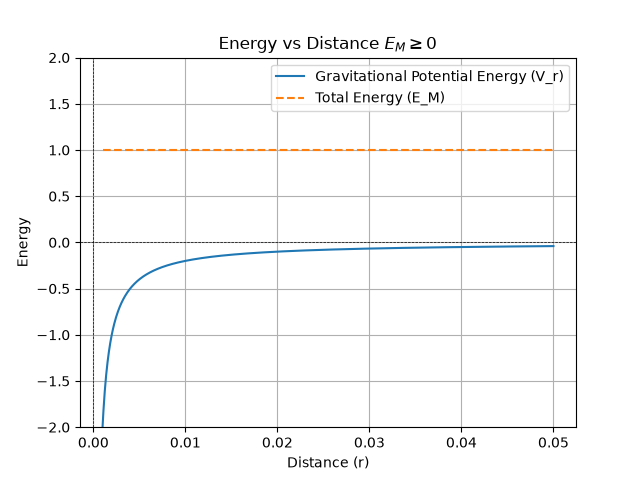
\includegraphics[width=\linewidth]{img/energy_vs_distance.png}
        \caption{Caso con $P = 0$ e $E_M \geq 0$}
        \label{fig:energiaPOtenzialeInFunzioneDiR}
    \end{subfigure}
    \hfill
    \begin{subfigure}[b]{0.48\textwidth}
        \centering
        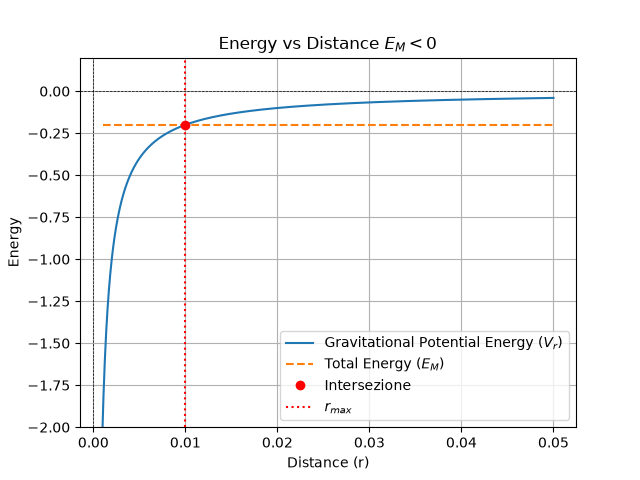
\includegraphics[width=\linewidth]{img/energy_vs_distance_negativa.png}
        \caption{Caso con $P = 0$ e $E_M < 0$}
        \label{fig:energiaPOtenzialeInFunzioneDiRNegativa}
    \end{subfigure}
    
    % Didascalia e label generali per l'intera figura
    \caption{Energia potenziale in funzione della distanza per $P = 0$.}
    \label{fig:energiaPotenzialeConfronto}
\end{figure}

\newpage

\paragraph{Caso $P \not = 0$}
Nel caso più interessante ove $P \not = 0$ il termine centrifugo $V_c(r)$ garantisce la stabilità del sistema, infatti la somma dei due termini $V_c(r) + V(r)$ garantisce la presenza di una "barriera" di potenziale per piccoli valori di $r$ dovuta a $V_c$ mentre per grandi valori di $r$ domina $V(r)$, come è possibile vedere in figura \ref{fig:energiaPOtenzialeInFunzioneDiRPNonNullo} $V_{eff}$ ha un minimo per $r = r_c$ e sia il valore del minimo che $r_c$ dipendono da $P$.

\begin{figure}[h]
    \centering
    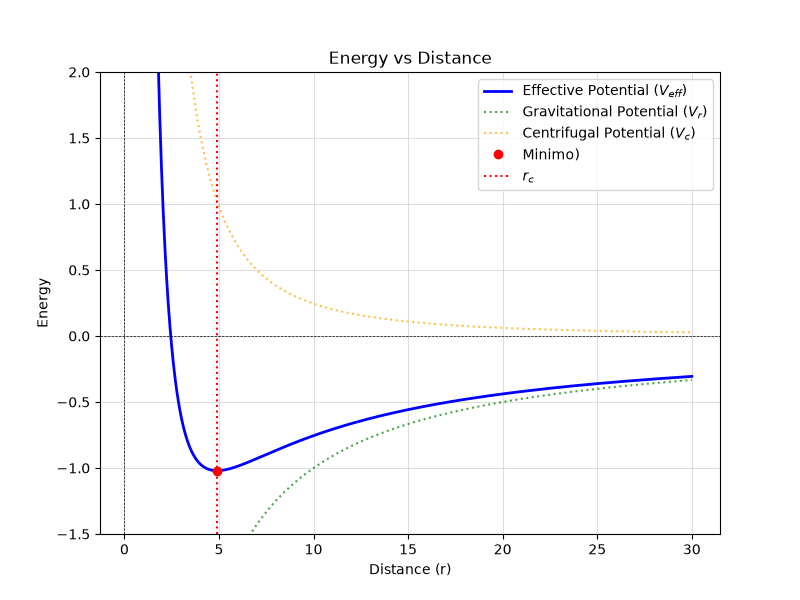
\includegraphics[width=\linewidth]{img/energy_vs_distance_pnonnullo.png}
    \caption{Caso con $P \not = 0$}
    \label{fig:energiaPOtenzialeInFunzioneDiRPNonNullo}
\end{figure}

Detta $E_c = V_{eff}(r_c)$ si possono verificare 3 casi:
\begin{itemize}
    \item $E_m < E_c$ moto impossibile.
    \item $E_c \leq E_m < 0$ il sistema si trova in uno stato legato.
    \item $E_m \geq 0$ il sistema non è legato.
\end{itemize}

\paragraph{Studio del sistema legato}
Nel caso in cui:
\begin{equation}
    E_c \leq E_M < 0
\end{equation}
le orbito sono limitate, in quanto il moto può avvenire solo per valori di r che soddisfano $r_{min} \leq r \leq r_{max}$.

Se $E_c < E_m < 0$ le traiettorie sono ellissi, con una eccentricità non nulla, mentre se $E_m = E_c$ si ha un moto circolare con raggio pari ad $r_c$
\paragraph{Studio del sistema non legato}
Nel caso in cui:
\begin{equation}
    E_M \geq 0
\end{equation}
il corpo è libero ma esiste una distanza minima $r_{min}$ di avvicinamento al secondo corpo e vale:
\begin{itemize}
    \item $E_M > 0$ le traiettorie sono iperboli.
    \item $E_M = 0$ le traiettorie sono parabole.
\end{itemize}

\subsection{Orbite circolari nel campo gravitazione}
Come già visto, questo caso corrisponde a $E_M = E_c$, vale che:
\begin{equation}
    P = mr_cv
\end{equation}
e poiché $P$ è costante, lo deve essere anche $v$, infatti il moto è circolare uniforme, come dimostrato delle leggi di Keplero.

Inoltre per questo moto vale che: $\dot{r} = 0$ da cui:
\begin{equation}
    E_M = V_{eff}(r_c) = -\frac{GMm}{r_c} + \frac{P}{2mr_c^2}
\end{equation}
nella quale $r_c$ corrisponde al minimo di $V_{eff}(r)$, calcolato imponendo la derivata prima di $V_{eff}$ uguale a 0, si trova in fatti che:
\begin{align}
    \dv{V_{eff}}{dr} & = 0 \\
                     & = \frac{GMm}{r_c^2} - \frac{P^2}{mr_c^3} = 0 \\
                     & = r_c = \frac{P^2}{GMm^2}
\end{align}
da cui vale che:
\begin{align}
    V(r_c) & = - \frac{GMm}{r_c} = - \frac{GMm^2r_c}{mr_c} = - 2 \frac{P^2}{2mr_c^2}\\
\end{align}
siccome $\frac{P^2}{2mr_c^2} = K$ essendo il termine $\frac{1}{2}m\dot{r}^2 = 0$, allora è possibile scrivere:
\begin{equation}
    V = -2K \implies K = -\frac{V}{2} = \frac{GMm}{2r_c}
\end{equation}
da cui segue che:
\begin{equation}
    E_M = K + V = - K = - \frac{1}{2}\frac{GMm}{r_c}
\end{equation}

\paragraph{Calcolo della velocità di fuga}
Per calcolare la velocità minima che si deve imprimere a un corpo affinchè esso si allontani indefinitamente dalla terra, bisogna considerare che un corpo si allontana indefinitamente se la sua energia meccanica iniziale è maggiore o uguale a 0.

Più intuitivamente il corpo non rimane legato alla terra se, a distanza "infinita" dove $V \to 0$, la sua energia cinetica è $\geq 0 $, la velocità di fuga corrisponde al caso limite $E_M = 0$.

Da cui:
\begin{equation}
    E_M = K_i + V_i = K_\infty + V_\infty = K_\infty \geq 0
\end{equation}
e la velocità di fuga corrisponde a $K_i + V_i = 0$
Pertanto:
\begin{equation}
    \frac{1}{2}mv^2_f - \frac{GMM_t}{R_t} = 0 \implies v_f = \sqrt{\frac{2GM_t}{R_t}}
\end{equation}
Da ciò è possibile determinare il raggio a cui corrisponde una velocità di fuga pari alla velocità della luce nel vuoto, infatti:
\begin{equation}
    R_S = \frac{2GM}{c^2}
\end{equation}
tale risultato è puramente classico non relativistico, discusso per la prima volta da J. Michell, ma e lo si combina con il fatto (non classico) che $c$ è una velocità limite, allora nessun corpo può abbandonare $M$ se il raggio è $\leq R_S$

\newpage
\section{Equazione canonica dell'ellisse in coordinate polari}
Scegliendo come origine il fuoco $F_2$ è possibile esprimere la distanza di un punto generico $p$ dai due fuochi in coordinate polari, tramite la seguente formula:

\begin{equation}
    \underbrace{\sqrt{(2c + r\cos\theta)^2 + r^2\sin^2\theta}}_{|\overline{PF_2}|} + \overbrace{r}^{|\overline{PF_1}|} = 2a
\end{equation}

\begin{figure}[h]
    \centering
    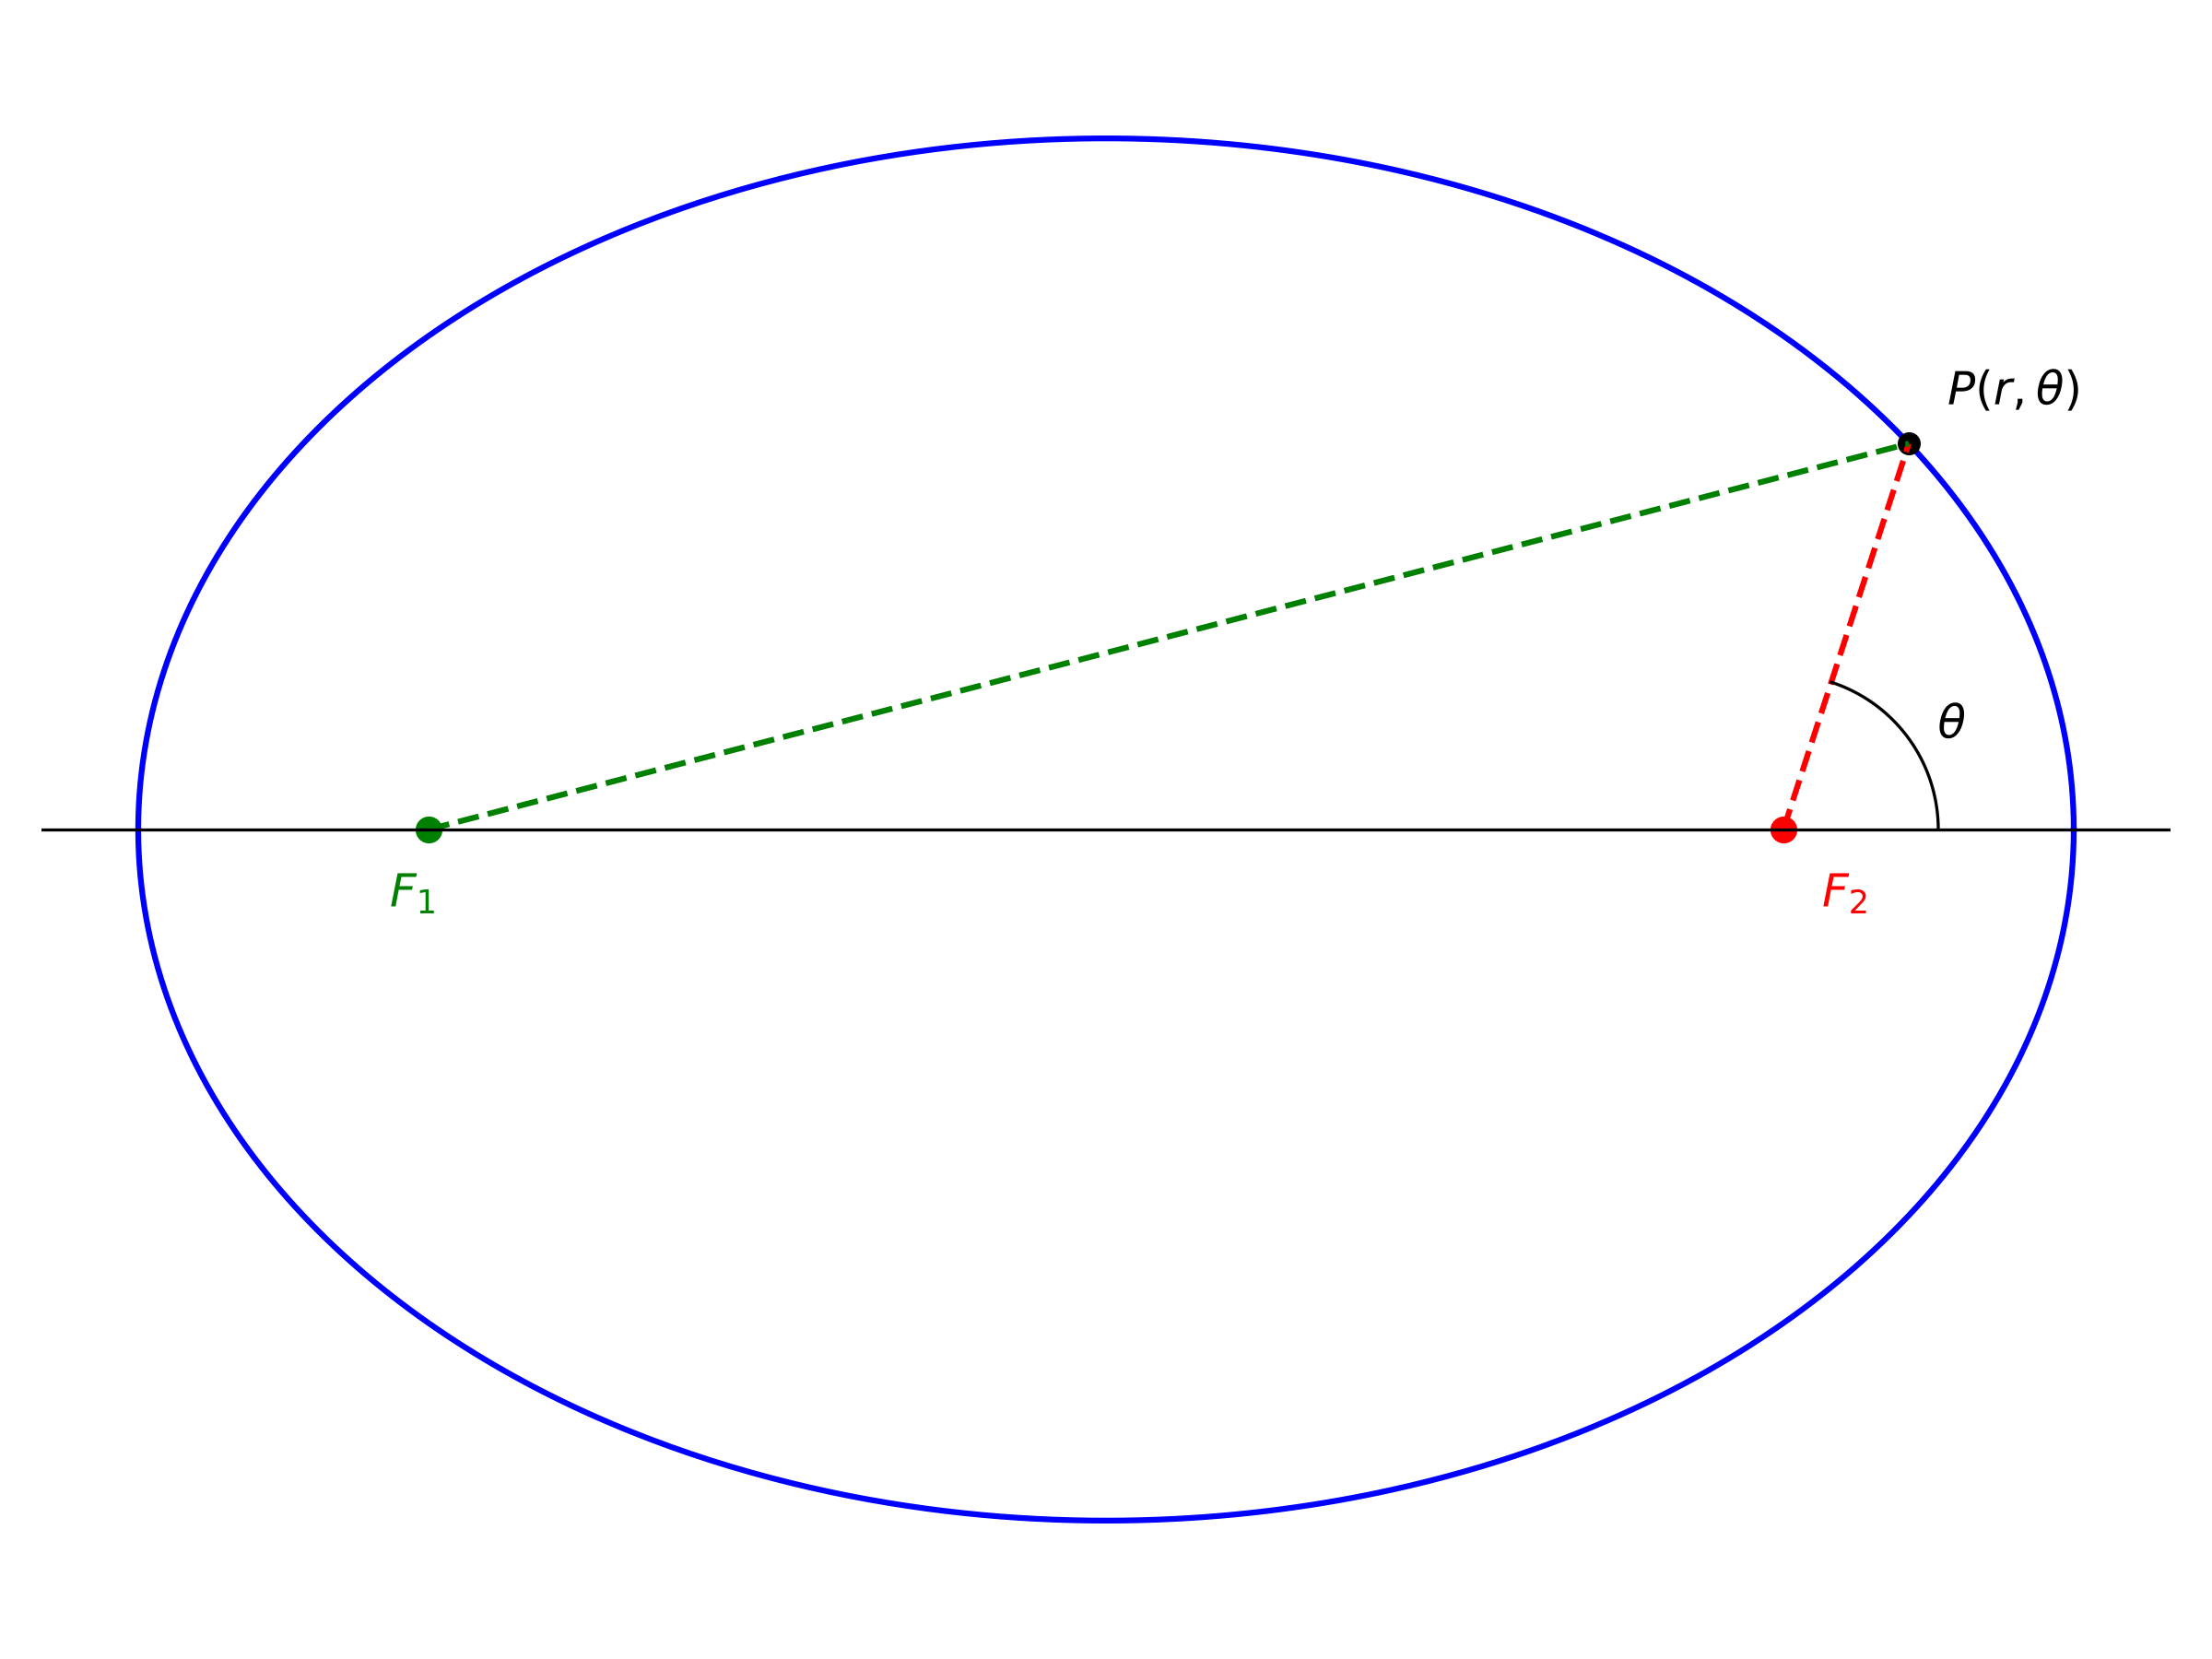
\includegraphics[width=0.7\linewidth]{img/ellissePolare.png}
    \caption{Ellisse con $F_2$ all'origine del sistema di riferimento polare.}
    \label{fig:ellissePolare}
\end{figure}

da cui segue che:
\begin{align}
    \sqrt{(2c + r\cos\theta)^2 + r^2\sin^2\theta} + r & = 2a \\
    \sqrt{(2c + r\cos\theta)^2 + r^2\sin^2\theta} & = 2a - r \\
    (2c + r\cos\theta)^2 + r^2\sin^2\theta & = (2a - r)^2 \\
    4c^2 + 4cr\cos\theta + r^2\cos^2\theta + r^2\sin^2\theta & = 4a^2 - 4ar + r^2 \\
    4c^2 + 4cr\cos\theta + r^2 & = 4a^2 - 4ar + r^2 \\
    4c^2 + 4cr\cos\theta & = 4a^2 - 4ar \\
    c^2 + cr\cos\theta & = a^2 - ar \\
    a^2 - b^2 + cr\cos\theta & = a^2 - ar \\
    cr\cos\theta & = b^2 - ar \\
    r(a + c\cos\theta) & = b^2 \\
    r(1 + e\cos\theta) & = \frac{b^2}{a}; \quad \quad \quad e = \frac{c}{a}
\end{align}

Introducendo la quantità:
\begin{equation}
    d := \frac{b^2}{ea}
\end{equation}
allora:
\begin{equation}
    r = ed - er\cos\theta \implies e = \frac{r}{d - r\cos\theta}
\end{equation}
tale equazione permette di definire un'altra definizione equivalente di ellisse, infatti l'ellise è il luogo dei punti del piano le cui distanza da un punto (il fuoce $F_2$) e da una retta (direttrice) giacenti nel piano hanno un rapporto costante $e < 1$

\subsection{Sistema Sole-Pianeta}
Sapendo che:
\begin{equation}
    r = \frac{b^2}{a(1 + e\cos\theta)}
\end{equation}
allora è possibile introdurre due quantità, l'afelio e il perielio, defini come segue:
\begin{equation}
    \begin{cases}
        \displaystyle \text{perielio}: & \theta = 0, r_p = \frac{b^2}{a(1 + e)} \\
        \displaystyle \text{afelio}:   & \theta = \pi, r_a = \frac{b^2}{a(1 - e)} 
    \end{cases}
\end{equation}

\begin{figure}[h]
    \centering
    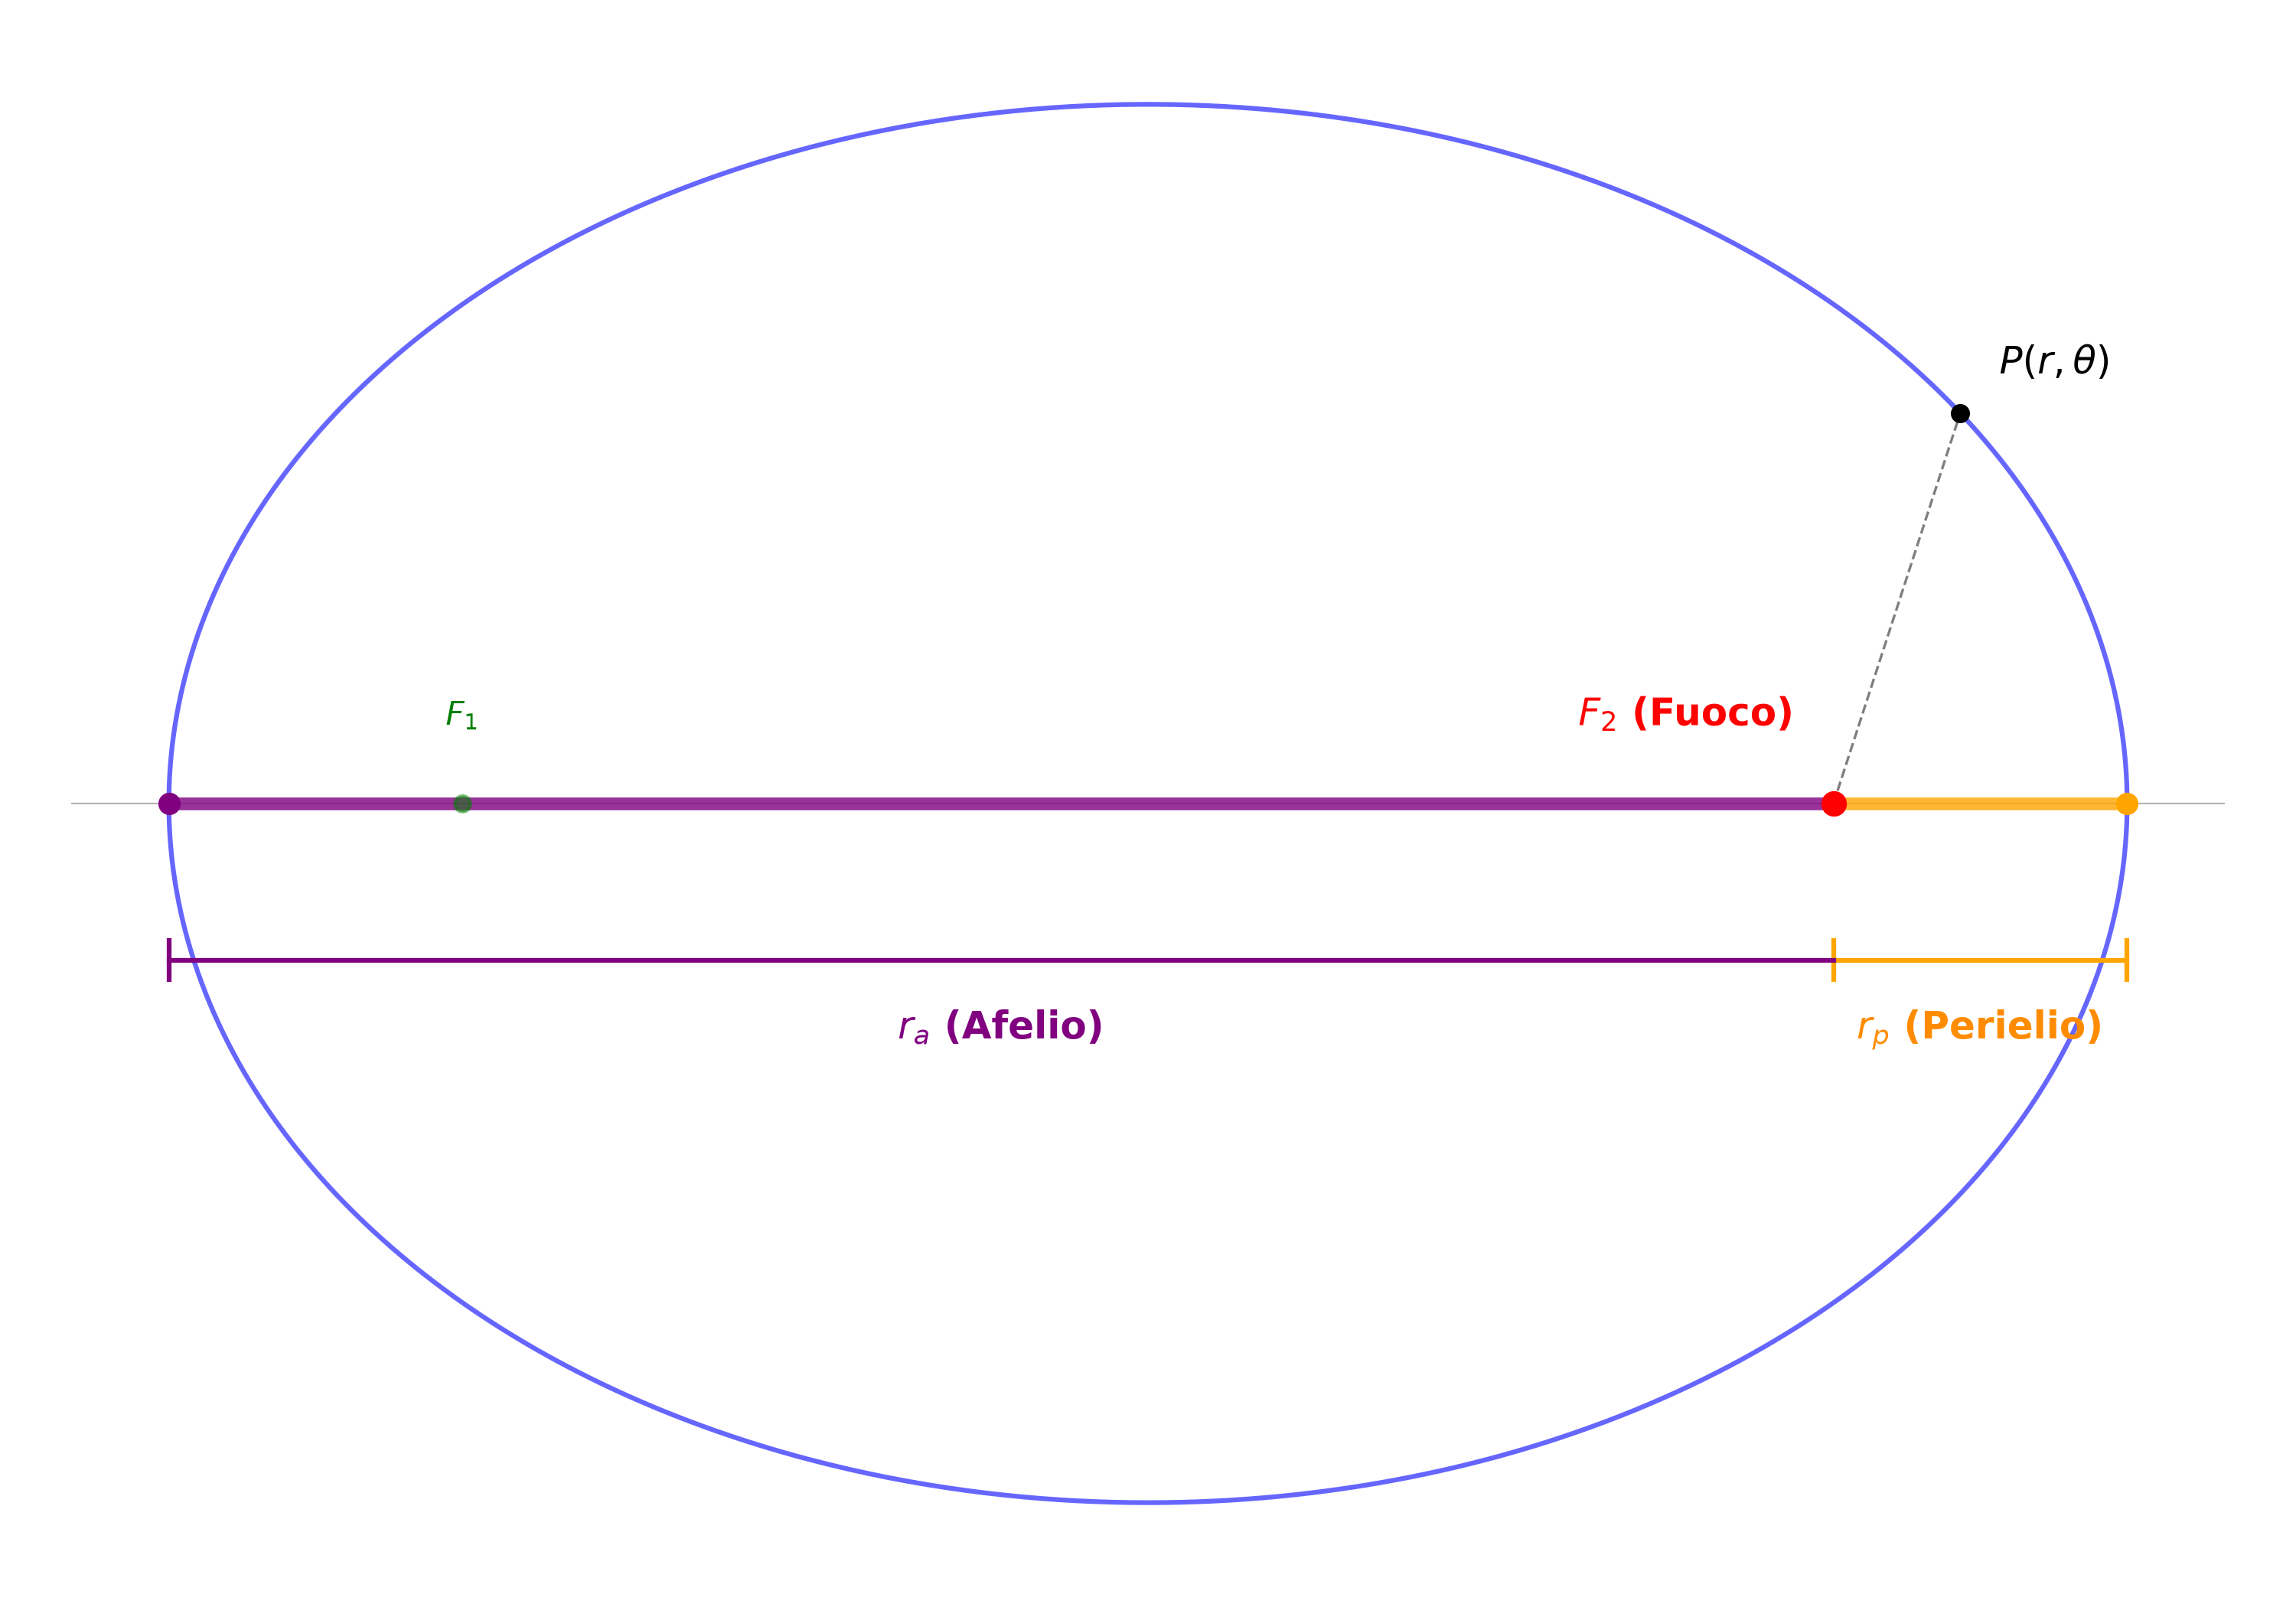
\includegraphics[width=0.7\linewidth]{img/ellissePerielioAfelio.png}
    \caption{Ellisse con $F_2$ all'origine del sistema di riferimento polare con rappresentazione delle distanza tra $F_2$ e il punto di perielio e il punto di afelio}
    \label{fig:ellissePerielioAfelio}
\end{figure}

da cui:
\begin{equation}
    r_p = \frac{a^2 - c^2}{a(1 + e)} = \frac{a^2(1 - e^2)}{a(1 + e)} = a(1 - e)
\end{equation}
\begin{equation}
    r_a = \frac{a^2 - c^2}{a(1 - e)} = \frac{a^2(1 - e^2)}{a(1 - e)} = a(1 + e)
\end{equation}
segue quindi che:
\begin{equation}
    a = \frac{1}{2}(r_a + r_p); \quad \quad e = \frac{r_a - r_p}{r_a + r_p}
\end{equation}

\section{Nota sulle curve coniche}
Le curve coniche possono essere definite come i luoghi dei punti del piano le cui distanza da un punto (fuoco) e da una retta (direttrice) giagenti nel piano hanno un rapporto costante $e$, le 3 curve corrispondono a:
\begin{equation}
    \begin{cases}
        0 \leq e < 1 & ellise (cerchio se e = 0) \\
        e = 1 & parabola \\
        e > 1 & iperbole
    \end{cases}
\end{equation}

\section{Dimostrazione I legge di Keplero}
È quindi possibile dimostrare che un corpo celeste soggetto all'atrtazione gravitazionale del Sole traccia una curva conica, la prima legge di Keplero corrisponde al caso di moto legato con traiettoria ellittica, poiché $P \not = 0$ allora esiste una distanza minima dal sola, ovvero il perielio.

In corrispondenza del perielio vale che:
\begin{equation}
    \dot{r} = 0
\end{equation}
e quindi $\vec{v} \perp \hat{u}_r$, per il II principio di Newton vale:
\begin{equation}
    m\dv{\vec{v}}{dt} = - \frac{\alpha}{r^2}\hat{u}_r
\end{equation}
da cui sapendo che:
\begin{equation}
    \hat{u}_r = -\dv{\hat{u}_\theta}{\theta} = -\dv{\hat{u}_\theta}{t}\dv{t}{\theta}
\end{equation}
ciò implica che:
\begin{equation}
    m\dv{\vec{v}}{t} = \frac{\alpha}{r^2\dot{\theta}} \dv{\hat{u}_\theta}{t} = \frac{\alpha m}{p}\dv{\hat{u}_\theta}{t} 
\end{equation}
da cui:
\begin{equation}
    \dv{}{t} \left(m\vec{v} - \frac{\alpha m}{p}\hat{u}_\theta\right) = 0
\end{equation}

Pertanto la quantità:
\begin{equation}
    \frac{p}{\alpha}\vec{v} - \hat{u}_\theta
\end{equation}
è una costante del moto.

Nella posizione del perielio è facile calcolare questa costante poiché $\vec{v} \parallel \hat{u}_\theta$, vale quindi che:
\begin{equation}
    \frac{p}{\alpha}\vec{v} - \hat{u}_\theta = e\hat{\jmath}
\end{equation}
moltiplicando scalarmente per $\hat{u}_\theta$ si ottiene:
\begin{equation}
    \frac{p}{\alpha}r\dot{\theta} - 1 = e\cos\theta \implies r(1 + e\cos\theta) = \frac{p^2}{m\alpha}
\end{equation}
da cui si legge che la traiettoria è una conica.

È possibile esprimere l'eccentricità in funzione delle costanti del moto $E_M$ e $p$, e per farlo è possibile calcolarla prima nel perielio, e vale:
\begin{equation}
    E_M = V_{eff}(r_p) = \frac{p^2}{2mr^2_p} + V(r) = \frac{p^2}{2mr^2_p} - \frac{\alpha}{r_p}
\end{equation}
usando le relazioni trovate precedentemente, si ottiene:
\begin{equation}
    p^2 = m\alpha(1 + e)r_p
\end{equation}
pertanto segue che:
\begin{equation}
    E_M = \frac{m\alpha(1 + e)r_p}{2mr_p^2} - \frac{\alpha}{r_p} = \frac{\alpha(e - 1)}{2r_p}
\end{equation}
esprimendo $r_p$ in funzione di $p^2$, si ricava:
\begin{equation}
    E_M = \frac{m\alpha^2(e^2 - 1)}{2p^2}
\end{equation}
ovvero:
\begin{equation}
    e = \sqrt{1 + \frac{2p^2E_M}{m\alpha^2}}
\end{equation}
Tale relazione permette di dimostrare la relazione fra $E_M$ e il tipo di traiettoria conica tracciata dal corpo, ovvero:
\begin{equation}
    \begin{cases}
        E_M < 0 & \implies e < 1: \text{ellisse} \\
        E_M = 0 & \implies e = 1: \text{parabola} \\
        E_M > 0 & \implies e > 1: \text{iperbole} \\
    \end{cases}
\end{equation}

È infine possibile esprimere l'energia meccanica in funzione del semiasse maggiore, nel di $E_M < 0$, infatti:
\begin{equation}
    r_p = \frac{p^2}{m\alpha(1 + e)}
\end{equation} 
\begin{equation}
    r_a = \frac{p^2}{m\alpha(1 - e)}
\end{equation} 
allora:
\begin{equation}
    2a = r_p + r_a = \frac{2p^2}{m\alpha(1 - e^2)}
\end{equation}
da cui:
\begin{equation}
    E_M = \frac{m\alpha^2(e^2 - 1)}{2p^2} = -\frac{\alpha}{2a} = -\frac{GM_sm}{2a}
\end{equation}

\section{Dimostrazione III legge di Keplero (caso generale)}
I risultati ottenuti dalla prima legge, permettono di dimostrare la III legge per il caso generale, infatti essendo la velocità aereolare costante e pari a:
\begin{equation}
    \sigma = \frac{p}{2m}
\end{equation}
allora il periodo del moto è:
\begin{equation}
    T = \frac{A}{\sigma} = \frac{\pi a b}{\sigma} = \frac{\pi a^2 \sqrt{1 - e^2}}{\sigma}
\end{equation}

sfruttando la relazione tra l'energia meccanica ed $a$, allora:
\begin{align}
    T^2 & = \frac{\pi^2a^4(1 - e^2)}{\sigma^2} \\
        & = \frac{\pi^2a^4(1 - e^2)4m^2}{p^2} \\
        & = \frac{\pi^2a^4(1 - e^2)4m^2}{am\alpha(1 - e^2)}  \\
        & = \frac{\pi^2a^3 4m}{\alpha} \\
    \implies \frac{T^2}{a^3} & = \frac{4\pi^2m}{GM_sm} = \frac{4\pi^2}{GM_s}
\end{align}


% INSERIRE TRAIETTORIE DI HOOMAHNN


\chapter{Meccanica dei fluidi}
Un fluido può essere definito in maniera intuitiva (ma non propriamente rigorosa) come un sistema materiale la cui forma è fissata da vincoli esterni, ovvero il recipiente che lo contiene.

A questa categoria appartengono i liquidi e i gas. Nel caso dei gas, il recipiente determina anche il volume, pertanto i gas sono un sistema a volume variabile e comprimibile, i liquidi al contrario hanno un volume proprio che dipende debolmente dalla temperatura e molto debolmente dalla pressione.

A livello microscopico tale comportamento è dovuto a interazioni molecolari più intense nei liquidi rispetto ai gas, ma comunque meno intense rispetto ai solidi.

È possibile trattare i fluidi in modo macroscopico, dividendo tali sistemi in porzioni "piccole" ma contenenti un numero enorme di costituenti microscopici, quindi verrano trattati come sistemi continui.

È possibile inoltre dare un definizione più precisa di fluido in termini dell'effetto che le forze tangenziali (ovvero le forze che tendono a far scorrere uno strato del sistema sull'altro) hanno su di essi.
Infatti per un fluido tale forze deformano il sistema con \textit{continuità} indipendetemente dalla loro intensità, al contrario in un solido le forze tangenziali provocano deformazioni finite, che non crescono indefinitamente.

\section{Densità nei fluidi}
Per lo studio dei fluidi è importante definire il concetto di densità, ne esistono 3 tipologie:
\begin{itemize}
    \item Densità media di un fluido:
    \begin{equation}
        \rho_m := \frac{\Delta m}{\Delta V}
    \end{equation}
    \item Densità locale:
    \begin{equation}
        \rho = \lim_{\Delta V \to 0} \frac{\Delta m}{\Delta V} = \frac{dm}{dV}
    \end{equation}
    \item Densità relativa (all'acqua):
    \begin{equation}
        \rho_r = \frac{\Delta m}{\Delta m_{H_2O}}
    \end{equation}
    nella quale $\Delta m_{H_2O}$ è la massa di un volume di acqua (a pressione atmosferica e $T = 3.8\deg C$) uguale a quello del sistema.
    Vale:
    \begin{equation}
        \rho_r = \frac{\Delta m}{\Delta V}\frac{\Delta V}{\Delta m_{H_2O}} \implies \rho = \rho_r\rho_{H_2O}
    \end{equation}
    il motivo per cui si prende come riferimento l'acqua alla temperatura di $T = 3.8\deg C$ è che la densità dell'acqua ha un massimo a quella temperatura, tale comportamento è anomalo infatti normalmente nei fluidi la densità diminuisce con la temperatura.
\end{itemize}

\section{Forze nei fluidi}
Dato un elemento di fluido, è conveniente suddividere le forze esterne che agiscono su di esso in 2 categorie:
\begin{itemize}
    \item forze di superficie, dovute alle parti di fluido confinanti con l'elemento in questione, e possono essere considerate come forze di contatto.
    \item forze di volume proporzionali al volume $\Delta V$ dell'elemento considerato (per esempio forze gravitazioni o centrifughe, proporzionali a $\Delta m$ e quindi a $\Delta V$)
\end{itemize}

\subsection{Pressione}
Considerando una piccola superficie immaginaria $\Delta S$ all'interno del fluido, è possibile supporre che questa superficie corrisponda alla faccia di un piccole volume di fluido.
Le forze di superficie sulla faccia del volumetto sono dovute alle forze che le particelle microscopiche alla destra del volumetto esercitano su quelle all'interno.

In generale, la forza di superficie risultante ha un componente normale entrate $\Delta \vec{F}_n$ che tende a comprimere il volumetto e un componente tangente $\Delta \vec{V}_t$, allora è possibile definire la pressione media come segue:
\begin{equation}
    p_m = \frac{\Delta F_n}{\Delta S}
\end{equation}
La pressione in un punti si ottiene tramite un processo di limite:
\begin{equation}
    p = \lim_{\Delta S \to 0} \frac{\Delta F_n}{\Delta S} = \frac{dF_n}{dS}
\end{equation}
è possibile dimostrare che il valore di $p$ non dipende dall'orientazione delle superficie. 
In generale le forze normali responsabili delle pressione sono presenti sia in condizioni statiche che in condizioni dinamiche. Esse sono dovute agli urti che le molecole esterne al volumetto esercitano sulla superficie considerata. Naturalmente, per il principio di azione e reazione, le particelle esercitano su quella a destra una reazione uguale e contraria.

L'unità di misura della pressione è il Pascal e vale che:
\begin{equation}
    1 Pa = 1 N \cdot m^{-2}
\end{equation}
altre unità di misura frequentemente usate sono il bar $1 bar = 10^5 Pa$ e l'atmosfera $1 atm = 1.013 \times 10^5 Pa$

La componente tangenziale della forza di superficie si definisce in maniera analoga alla pressoine, ed è definita come \textit{sforzo di taglio} $\vec{T}$:
\begin{equation}
    \vec{T} := \frac{d\vec{T}_t}{dS}
\end{equation}
In generale gli sforzi di taglio sono presenti solo se il fluido è in movimento, essi corrispondono intuitivamente a una forma di attrito interno che si manifesta quando una porzione di fluido è in moto rispetto alla porzioni confinanti, mentre dal punto di vista microscopico sono dovute a forze di coesione attrattive fra le molecole contenute negli elementi di fluido in moto l'uno verso l'altro.

\newpage

\section{Statica dei fluidi}
Per lo studio della statica dei fluidi è necessario considerare le forze di volume e le forze di superficie normali, poiché quelle tangenti sono nulle per fluidi fermi.

Nello specifico affinché ogni elemento di un fluido sia in quiete è necessario che la somma vettoriale delle forze precedentemente elencate, agenti sul corpo sia pari a 0.

Ad esempio, studiando un corpo sul quale agisce solo la forza peso (una forza di volume), poiché tale forza è verticale, è possibile considerare un elemento di fluido cilindrico, (considerandolo come se fosse una superficie immaginaria a forma di moneta) per via della simmetria cilindrica le forze normali agenti sulla superficie laterale dovute alla pressione si annullano, è quindi necessario tener conto soltanto delle forze normali sulle basi, di area $A$, della superficie immaginaria e della forza peso.

poiché è presente la forza peso, allora la pressione dipende dalla coordinata $z$. Detto quindi $dz$ lo spessore infinitesimo della moneta, deve valere in condizione di equilibrio che:
\begin{equation}
    -\rho Agdz -p(z + dz)A + p(z)A = 0 
\end{equation}
usando il seguente sviluppo di Taylor al primo ordine:
\begin{equation}
    p(z + dz) = p(z) + \frac{dp}{dz}dz
\end{equation}
segue che:
\begin{align}
    -\rho Agdz -(p(z) + \frac{dp}{dz}dz)A + p(z)A & = 0 \\
    -\rho Agdz - \frac{dp}{dz}Adz & = 0
\end{align}
dividendo per il volume $Adz$, segue che:
\begin{equation}
    \frac{dp}{dz} = -\rho g
    \label{eq:relazioneDerivataDellaPressione}
\end{equation}
o in forma vettoriale:
\begin{equation}
    \vec{\nabla}p = \rho\vec{g}
\end{equation}
Tale formula può essere generalizzata al caso in cui sono presenti più forze di volume, aventi componenti non nulle lungo i 3 assi.

Nel caso più generale è possibile applicare le precedenti considerazioni in presenza di un volumetto cubico infinitesimo, tenendo presente che la pressione può dipendere da $x,y,z$. Imponendo che tutte le componenti della forza complessiva siano nulle, allora si ottiene:
\begin{equation}
    \vec{\nabla}p = \rho\vec{H}
\end{equation}
dove $H$ è la risultante delle forze di volume per unità di massa, quindi $\vec{H}$ è il rapporto fra la forza di volume totale $\vec{F}_V$ agente su un volumetto e la massa $\Delta m$ del volumetto stesso:
\begin{equation}
    \vec{H} = \frac{\vec{F}_V}{\Delta m} \implies \vec{F}_V = \Delta m \vec{H} = \rho\Delta V \vec{H} 
\end{equation} 
segue quindi che $\vec{H}$ ha le dimensioni di una accelerazione, le cui componenti sono:
\begin{equation}
    \begin{cases}
        \displaystyle \pdv{p}{x} & = \rho H_x \\[1em]
        \displaystyle \pdv{p}{y} & = \rho H_y \\[1em]
        \displaystyle \pdv{p}{z} & = \rho H_z \\
    \end{cases}
\end{equation}

Se $\vec{H}$ è conservativa, allora è possibile definire un potenziale per unità di massa $\Phi(r)$, è possibile infine scrivere:
\begin{equation}
    \vec{\nabla}p = -\rho \vec{\nabla}\Phi
\end{equation}
Tale formula mostra che le superfici a pressione costante, dette isobariche, coincidono con quelle equipotenziali.

Nel caso in cui è presente solo la forza peso, le superfici isobariche sono piane e orizzontali (se si considera una sezione di spazio in cui $\vec{g}_i \approx -g\hat{k}$)
 
\paragraph{Esempio: Trovare le superfici equipotenziali di un corpo soggetto a forza peso e forza centrifuga:} Per trovare le superfici isobariche di un liquido di densità $\rho$ che si trova all'interno di un recipiente cilindrico e che ruota solidalmente al recipiente attorno ad un asse verticale con velocità angolare $\vec{\omega}$.

La forza che agisce su un elemento di liquido di massa $\delta m$ è pari alla somma vettoriale della forza peso e della forza centrifuga, da cui segue che:
\begin{equation}
    \vec{H} = \frac{\vec{F}_v}{\Delta m} = \vec{g} + \omega^2\xi 
\end{equation}
con $\xi$ definite come la distanza perpendicolare tra l'asse e l'elemento $dm$.

L'energia potenziale per unità di massa è quindi:
\begin{equation}
    \Phi(\vec{r}) = gz - \frac{1}{2}\omega^2\xi^2, \quad \quad \xi^2 = x^2 + y^2
\end{equation}

Le superfici isobariche corrispondono quindi alle superfici equipotenziali:
\begin{equation}
    gz = \frac{1}{2}\omega^2(x^2 + y^2) + c
\end{equation}
tali figure sono parabolidi di rotazione.

\subsection{Legge di Stevino e Principio di Pascal}
Considerando un liquido soggetto alla forza peso e assumendo che la sua densità non dipende ne dalla pressione ne dalla temperatura, effettuando l'approssimazione di liquido incompressibile (che per molti problemi è adeguata) è possibile integrando l'equazione \ref{eq:relazioneDerivataDellaPressione} si ottiene:
\begin{equation}
    p_2 - p_1 = -\rho g(z_2 - z_1)
    \label{eq:relazioniPressioneAltezze}
\end{equation}
tale formula afferma che la variazione di pressione fra due punti è data dalla loro differenza in quota moltiplicata per $-\rho g$.

Indicando con $p_0$ la pressione alla superficie libera di un liquido e con p il valore ad una profondità $h$, allora si ottiene:
\begin{equation}
    p = p_0 + \rho gh
    \label{eq:LeggeDiStevino}
\end{equation}
tale equazione è detta \textbf{Legge di Stevino}, e la quantità $\rho gh$ è detta pressione idrostatica.

La pressione idrostatica corrisponde alla pressione dovuta al peso di una colonna di liquido di altezza $h$ e di area di base $A$, tale peso è distribuito sulla base della colonna, da cui:
\begin{equation}
    p_{idr} = \frac{\rho gh A}{A}
\end{equation}

Dalla \ref{eq:LeggeDiStevino} si ricava il principio di Pascal.
\begin{theorem}[Principio di Pascal]
    In un fluido incompressibile in quiete, un incremento di pressione prodotto in un punto di propaga inalterato in ogni altro punto del fluido.
\end{theorem}


\paragraph{Applicazioni del principio di Pascal}
Le principali applicazioni del principio di Pascal sono la pressa idraulica che si comportan da moltiplicatore di forza, e i freni delle automobili.

\subparagraph{Pressa idraulica}
Consideriamo un sistema dotato di due superfici mobili di area $A_{in}$ e $A_{out}$, dove $A_{in} < A_{out}$. Applicando una forza $F_{in}$ sulla superficie d'ingresso $A_{in}$, si genera all'interno del fluido una pressione pari a:
\begin{equation}
    p = \frac{F_{in}}{A_{in}}
\end{equation}

Per il principio di Pascal, tale pressione $p$ si trasmette integralmente fino alla superficie d'uscita $A_{out}$. La forza emergente $F_{out}$ esercitata dal fluido su quest'ultima superficie sarà quindi:
\begin{equation}
    F_{out} = p \cdot A_{out}
\end{equation}

Sostituendo l'espressione della pressione $p$ trovata in precedenza, otteniamo la relazione fondamentale della pressa idraulica:
\begin{equation}
    F_{out} = \left( \frac{F_{in}}{A_{in}} \right) A_{out} = \frac{A_{out}}{A_{in}} F_{in}
\end{equation}

Poiché, per ipotesi di costruzione, l'area di uscita è maggiore dell'area di ingresso ($A_{out} > A_{in}$), il rapporto geometrico $\frac{A_{out}}{A_{in}}$ risulta maggiore di 1. Di conseguenza, la forza in uscita è sempre maggiore della forza applicata in entrata:
\begin{equation}
    F_{out} > F_{in}
\end{equation}
Questo dimostra come la pressa idraulica agisca a tutti gli effetti come un moltiplicatore di forza.

\subsection{Pressione atmosfera}
L'aria è un fluido e quindi è caratterizzata da una pressione che dipende dalla quota, tale pressione può essere misurata usando il barometro, strumento inventato da Torricelli.

Il liquido utilizzato è il mercurio, l'equilibrio la pressione nei punti A e B deve essere la stessa, in quanto i due punti sono alla stessa quota.

La pressione in A corrisponde a quella atmosfera, mentre in B è la pressione idrostatica dovuta alla colonna di mercurio di altezza $h$ (tendendo conto che la pressione $p_0$ alla superficie libera, dovuta ai vapori di mercurio è piccola), uguagliando quindi le due presioni si ottiene:
\begin{equation}
    P_{atm} = \rho_{mercurio} g h
\end{equation}
A livello del mare la colonna di mercurio è alta circa $76cm$ (tale valore non è costante in quanto la pressione atmosferica varia in funzione delle condizioni atmosferiche), da ciò segue che:
\begin{equation}
    P_{atm} = \rho_{mercurio} \frac{kg}{m^3} \cdot 9.81 \frac{m}{s^2} \cdot 0.76 m \simeq 1.013 \cdot 10^5 Pa
\end{equation}
Tale pressione corrisponde per definizione all'unità di misura dell'atmosfera. Esiste anche un'altra unità di misura molto utilizzata, il Torr, che corrisponde alla pressione di una colonna di mercurio di $1 mm$, da cui segue che:
\begin{equation}
    1 atm = 760 \text{ } Torr
\end{equation}

\subsection{Dipendenza della pressione atmosferica dalla quota}
Usando la relazione \ref{eq:relazioneDerivataDellaPressione} è possibile calcolare la dipendenza della pressione atmosferica dell'aria dalla quota.
Trattandosi di un gas, non è possibile assumera che la sua densità sia costante, quindi non si può usare la legge di Stevino.

Per risolvere tale problema è necessario usare oltre alla \ref{eq:relazioneDerivataDellaPressione} anche un'altra equazione che metta in relazione $\rho$ e $p$ dato che non si conosce a priprio la dipendenza di $\rho$ da $z$.

Si può dimostrare che, per i gas rarefatti come l'aria, vale con buono approssimazione che:
\begin{equation}
    pV \propto T
    \label{eq:leggeDelGasPerfetto}
\end{equation}
dove $V$ è il volume occupato dal gas e $T$ e la sua temperatura, tale formula è detta la legge del gas perfetto, se si vuole esprimere in funzione della densità, vale che:
\begin{equation}
    \frac{p}{\rho} \propto T
\end{equation}

Come è noto la temperatura dell'aria dipende anch'essadalla quota, ma per variazioni non troppo grandi della quota è possibile, in prima approssimazione, considerarla costante. Si ottiene quindi:
\begin{equation}
    \frac{p}{\rho} = \text{costante}
\end{equation}

definendo come $p_0$ e $\rho_0$ i valori della pressione e della densità alla quota di base, allora:
\begin{equation}
    \frac{p}{\rho} = \frac{p_0}{\rho_0}
\end{equation}
sostituendo questa telazione in \ref{eq:relazioneDerivataDellaPressione} si ottiene:
\begin{equation}
    \frac{dp}{dz} = -p(z)\frac{\rho_0}{p_0} g \implies \frac{dp}{p} = - \frac{\rho_0}{p_0} g dz
\end{equation}

tale equazione differenziale può essere facilmente risolta intengrando entrambi i membri si ottiene:
\begin{equation}
    \int_{p_0}^{p} \frac{dp}{p} = = - \int_{0}^{z} \frac{\rho_0}{p_0}gdz \implies \ln(\frac{p}{p_0}) = - \frac{\rho_0}{p_0} g z 
\end{equation}
da cui segue che:
\begin{equation}
    p(z) = p_0e^{\displaystyle -\frac{\rho_0}{p_0}gz} = p_0 e^{\displaystyle -\frac{z}{\lambda}}; \quad \lambda := -\frac{gp_0}{\rho_0}
\end{equation}

Pertanto, la pressione diminuisce all'aumentare della quota in modo esponenziale.

Si può mostrare che, nei livelli bassi dell'atmosfera il valore di $\lambda$ è dell'ordine di $7-8km$, è importante notare che per tali valori di differenza di quota la temperatura dell'aria varia in modo non trascurabile (sapendo che, salendo, la temperatura diminuisce di circa $0.65 \deg$ ogni 100 metri).

\subsection{Principio di Archimede}

\begin{theorem}[Il principio di Archimede]
Il principio di Archimede, che dal punto di vista teorico è una legge derivabile dalle equazioni della statica dei fluidi, afferma che un corpo immerso parzialmente o totalmente in un fluido riceve da questo, in presenza di gravità, una spinta verticale verso l'alto il cui modulo è pari al peso del volume di fluido spostato.
\end{theorem}

\begin{proof}
    Per dimostrare il principio, immaginiamo di sostituire il corpo immerso con una porzione del medesimo fluido avente lo stesso identico contorno. Tale porzione di fluido si trova in equilibrio statico, pertanto la forza peso che agisce su di essa è perfettamente bilanciata dalla risultante delle forze di superficie esercitate dal fluido circostante sul suo contorno.
    
    Poiché queste forze di superficie dipendono unicamente dalla geometria del contorno e dalla distribuzione della pressione idrostatica esterna, esse non variano se al posto del fluido si inserisce il corpo vero e proprio. Di conseguenza, il corpo subisce la medesima spinta verso l'alto, uguale e opposta al peso del fluido spostato (ovvero la porzione di fluido avente un volume pari a quello della parte immersa del corpo).

    Se il corpo è immerso solo parzialmente, le stesse considerazioni geometriche e dinamiche si applicano alla sola frazione volumetrica sommersa.
\end{proof}

Dal principio di Archimede consegue che un corpo galleggia in un fluido se la sua densità media $\rho_c$ è inferiore a quella del fluido $\rho_f$.

Infatti, se il corpo fosse completamente immerso, la spinta di Archimede:
\begin{equation}
    \vec{A} = -\rho_f V \vec{g}
\end{equation}
sarebbe maggiore in modulo rispetto alla forza peso del corpo:
\begin{equation}
    \vec{F}_{p} = \rho_c V \vec{g}
\end{equation}
Poiché $\rho_f > \rho_c$, la forza risultante è diretta verso l'alto; il corpo quindi sale in superficie ed emerge parzialmente.

Una volta raggiunto l'equilibrio statico, la parte che rimane immersa riceve una spinta di Archimede che bilancia esattamente il peso totale del corpo, ovvero:
\begin{equation}
    A = \rho_f V_i g = \rho_c V g
\end{equation}
dove $V_i$ è il volume della parte immersa del corpo e $V$ è il suo volume totale. Da questa uguaglianza si ricava l'espressione per la frazione sommersa del corpo:
\begin{equation}
    \frac{V_i}{V} = \frac{\rho_c}{\rho_f}
\end{equation}

\subsection{Statica del galleggiamento}
Dalle considerazioni fatte precedentemente è possibile ricavare informazioni non solo sul modulo della spinta, ma anche sul suo punto di applicazione: per la seconda equazione cardinale, affinché il sistema sia in quiete, deve essere nullo anche il momento risultante delle forze esterne, oltre alla loro risultante.

Pertanto le forze superficiali sono equivalenti a una forza opposta alla forza peso, applicata nel baricentro del volume di fluido spostato.

\begin{proof}[Dimostrazione: Equivalenza delle forze superficiali]
Per determinare l'effetto delle forze di pressione, si applica il principio di sostituzione: si immagini di rimuovere il corpo immerso e di sostituire il suo volume $V$ con un'uguale quantità del fluido circostante, in quiete.
Questo volume di fluido, di massa $m_f$, si trova in equilibrio statico sotto l'azione del proprio peso $\vec{F}_{p, f} = m_f \vec{g}$, applicato nel suo baricentro geometrico $B$, e della risultante delle forze di pressione superficiali $\vec{F}_{\text{sup}}$ esercitate dal resto del fluido.
Dalla prima equazione cardinale si ha $\vec{F}_{\text{sup}} + \vec{F}_{p, f} = \vec{0}$, da cui $\vec{F}_{\text{sup}} = -\vec{F}_{p, f}$.
Calcolando i momenti rispetto al baricentro $B$ del fluido spostato, poiché il peso ha braccio nullo rispetto a $B$, si ottiene $\vec{M}_{B, \vec{F}_{{\text{sup}}}} = \vec{0}$. Questo dimostra che la spinta risultante $\vec{F}_{\text{sup}}$ è equivalente a un'unica forza applicata esattamente in $B$.
\end{proof}

Per il corpo immerso, la spinta di Archimede è quindi applicata nel punto che corrisponde al baricentro del liquido spostato, e non al baricentro del corpo: tale punto è detto \emph{centro di galleggiamento}

In condizioni statiche, la spinta di Archimede e la forza peso devono avere momento risultante nullo rispetto a un polo qualunque: ciò è verificato se e solo se le due forze hanno la stessa retta d'azione.

\begin{proof}[Dimostrazione: Allineamento delle rette d'azione]
Sul corpo rigido in quiete agiscono la forza peso $\vec{P}$, applicata nel centro di massa $G$, e la spinta di Archimede $\vec{S}$, applicata nel centro di galleggiamento $B$.
Scegliendo il centro di massa $G$ come polo, il momento della forza peso è nullo. Affinché il momento risultante sia nullo (seconda equazione cardinale), deve valere:
\begin{equation}
    \vec{M}_G = (\vec{r}_B - \vec{r}_G) \times \vec{S} = \vec{0} 
    \label{eq:momento_polo_G}
\end{equation}
Poiché $\vec{S}$ è un vettore non nullo e rigorosamente verticale (essendo $\vec{S} = -\vec{P}$), l'annullamento del prodotto vettoriale impone che il vettore posizione relativa $(\vec{r}_B - \vec{r}_G)$ sia parallelo a $\vec{S}$, dunque verticale. Di conseguenza, il segmento che unisce $G$ e $B$ deve essere verticale, ponendo i due punti sulla stessa retta d'azione.
\end{proof}

Tale studio ha un'applicazione nella progettazione delle imbarcazioni: infatti esse non devono solo essere in grado di galleggiare, ma devono anche trovarsi in una condizione di equilibrio stabile. Si possono distinguere due casi, a seconda della posizione relativa di $G$ e $B$:
\begin{itemize}
    \item \textbf{Centro di massa al di sotto del centro di galleggiamento}: in questo caso il sistema è sempre in equilibrio stabile, poiché per piccoli spostamenti dalla posizione di equilibrio i momenti delle due forze tendono a riportare il sistema in equilibrio.
    
    \begin{proof}[Dimostrazione (Stabilità con $G$ sotto $B$)]
    Poniamo che in condizioni di quiete $G$ si trovi sotto $B$ a una distanza $h > 0$. Definiamo $\vec{r}_{BG} := \vec{r}_B - \vec{r}_G$ il vettore posizione di $B$ rispetto a $G$, così che $\vec{r}_{BG} = h\hat{k}$, con $\hat{k}$ versore verticale verso l'alto.
    Se il corpo subisce una piccola rotazione oraria di angolo $\theta$ (nel piano $\hat\imath$-$\hat k$), il corpo è rigido e $B$ resta solidale ad esso, per cui $\vec{r}_{BG}$ ruota esattamente in
    $$ \vec{r}_{BG}' = h\sin\theta\hat{\imath} + h\cos\theta\hat{k}, $$
    dove $\hat{\imath}$ è il versore orizzontale nel piano di inclinazione. Il momento generato dalla spinta $\vec{S} = S\hat{k}$ rispetto a $G$ diventa:
    $$ \vec{M}_G = \vec{r}_{BG}' \times \vec{S} = (h\sin\theta\hat{\imath} + h\cos\theta\hat{k}) \times S\hat{k} = -hS\sin\theta\hat{\jmath} \label{eq:momento_stabilita} $$
    Il segno negativo indica che il momento risultante è opposto al verso della perturbazione: agisce quindi da momento di richiamo, e l'equilibrio è pertanto intrinsecamente stabile.
    \end{proof}
    
    \item \textbf{Centro di massa al di sopra del centro di galleggiamento}: in questo caso l'equilibrio non è garantito a priori. Se il sistema si inclina verso destra (sinistra), i momenti delle forze peso e spinta di Archimede tendono a riportare il sistema in posizione verticale se e solo se il nuovo centro di galleggiamento si trova a destra (sinistra) della retta d'azione della forza peso.
    
    \begin{proof}[Dimostrazione (Stabilità con $G$ sopra $B$)]
    Quando l'imbarcazione si inclina verso destra di un angolo $\theta$, la geometria della parte immersa cambia: il lato destro si immerge maggiormente, spostando il centro di galleggiamento verso destra, in una nuova posizione $B'$.
    La spinta di Archimede $\vec{S}$ agisce ora lungo la nuova verticale passante per $B'$. Il braccio di questa forza rispetto al centro di massa $G$ dipende dalla distanza orizzontale tra $G$ e tale verticale.
    Se lo spostamento di $B'$ è tale da portarlo strettamente a destra della retta d'azione del peso (passante per $G$), la spinta genera un momento raddrizzante, in senso antiorario rispetto a $G$. Viceversa, se $B'$ resta a sinistra della verticale di $G$, la spinta genera un momento ribaltante, in senso orario. Questo definisce la condizione di stabilità.
    \end{proof}
\end{itemize}
È importante notare che il centro di massa è solidale con il corpo, mentre la posizione del centro di galleggiamento dipende dalla forma della parte immersa, che varia al variare dell'inclinazione.

\section{Dinamica dei fluidi}
Per descrier enu fluido in movimento possono essere utilizzati due approcci diversi:
\begin{itemize}
    \item la descrizione \textit{lagrangiana}
    \item la descrizione \textit{euleriana}
\end{itemize}
\subsection{Descrizione lagrangiana}
La descrizione lagrangiana consiste nel fissare un sistema di riferimento e nel descrivere il moto delle singolo particelle del liquido in quel sistema di riferimento.

Pertanto, tale descrizione corrisponde all'approccio usato fino ad ora per studiare la dinamica dei sistemi.

Per questa descrizione è necessario individuare la posizione iniziale $x_0, y_0, z_0$ all'istante $t = 0$ degli elementi del fluido e determinare le loro traiettorie $x(t), y(t), z(t)$ risolvendo le opportune equazioni differenziali.

È possibile effettuare una analogia fra questa descrizione e il monitoraggio del moto, rispetto alla riva, di un galleggiante lascianto in un punto di un fiume all'intante $t = 0$, a ogni elemento del liquido corrisponde un'equazione oraria del tipo:
\begin{equation}
    \begin{cases}
        x = x(x_0, y_0, z_0, t) \\
        y = y(x_0, y_0, z_0, t) \\
        z = z(x_0, y_0, z_0, t) \\
    \end{cases}
\end{equation}

\subsection{Descrizione euleriana}
La descrizione euleriana consiste, al contrario di quella lagrangiana, nel determinare il moto di un fluido osservando un certo numero di posizioni, non vengono monitorate le traiettorie delle singole particelle ma vengono misurate le velocità delle particelle del fluido quando passano presso i punti d'osservazione.

Queste velocità si riferiscono a particelle di liquido sempre divere tra loro, pertanto in questa descrizione si definisce un cosiddetto, \textit{campo di velocità}:
\begin{equation}
    \vec{v} = \vec{V}(x, y, z, t)
\end{equation}  
dove $x, y, z$ determinano le coordinate del punto d'osservazione e $t$ è l'istante in cui la misura viene effettuata.

Un campo di velocità è un campo vettoriale, ovvero una funzione che associa ad ogni punto dello spazio considerato e ad ogni istante di tempo un vettore.

Tale descrizione è applicabile non solo alla velocità ma a tutte le grandezze fisiche che descrivono il moto (accelerazione, pressione, etc)

In questo corso verrà usato solo l'approccio euleriano che permette di classificare il moto due fluidi in stazionario e non stazionario.

\subsection{Moto stazionario}
Nel caso di moto stazionario, il campo delle velocità non dipende dal tempo:
\begin{equation}
    \vec{v} = \vec{v}(x, y, z)
\end{equation}
La stazionarietà del moto non implica che una determinata particella abbia velocità costante.

È quindi importante introdurre il concetto di linea di flusso e tubo di flusso.

\subsection{Linea di flusso}
Sopponendo che sia noto in un certo instante $t$ il campo delle velocità, allora si definisce la linea di flusso come una linea geometrica tangente in ogni punto alla velocità nel punto stesso. 

Le linee di flusso sono particolarmente utili nello studio di moti stazionari.

infatti, in questo caso, esse non dipendono dal tempo e corrispondono alle traiettorie reali delle particelle.

Le linee di flusso non si possono intersecare fra loro, altrimenti si avrebbero particelle con due velocità diverse nel punto di intersezione.

\subsection{Tubo di flusso}
Nel caso di moti stazoinari, è utile introdurre il concetto di tubo di flusso.

Un tubo di flusso è una superficie formata dalle linee di flusso che passano per i punti di una data linea chiusa.

Il tubo di flusso separa il fluido in una parte interna e una esterna, e non vi è scambio di particelle fra le due parti, in quanto, se così fosse, vi sarebbero intersezioni fra le linee di campo. Vale quindi che le linee di campo sono quindi "impermeabili" rispetto alle porzioni di fluido che li circondano.

\subsection{Classificazione dei fludi e del tipo di moto}
Classificazione basata sulle proprietà fisiche:
\begin{itemize}
    \item Fluido incompressibile, ovvero fluido a densità costante (buona approssimazione per i liquidi)
    \item Fluido non viscono, ovvero un fluido con sforzo di taglio nullo anche in condizioni di moto
\end{itemize}
Un fluido incompressibile e non viscoso è detto prefetto o ideale.

Classificazione basata sulle caratteristiche del moto:
\begin{itemize}
    \item Moto stazionario:
    \begin{equation}
        \vec{v}(x, y, z)
    \end{equation}
    indipendente dal tempo
    \item Moto irrotazionale:
    \begin{equation}
        \vec{\nabla} \times \vec{v} = 0
    \end{equation}
    nel caso di spazi con domini semplicemente connessi, implica che non vi sono vortici.
\end{itemize}

\newpage

\section{Analisi dei moti stazionari}
È necessario che, nello svolgeri del moto, la massa si conservi, infatti è possibile derivare un'equazione di continuità che appunto esprime la conservazione della massa.
\subsection{Equazione di continuità}
Considerando un tupo di flusso sottile, prendendo la porzione di fluido limitate dalle basi $A_1$ e $A_2$ corrispondeti al tempo $t$, indicando con $\rho_1$ e $\rho_2$ e  con $v_1$ e $v_2$ le densità e le velocità del fluido in corrispondenza delle 2 basi, come si vede in figura \ref{fig:tubiDiFlusso}.

\begin{figure}[h!]
    \centering
    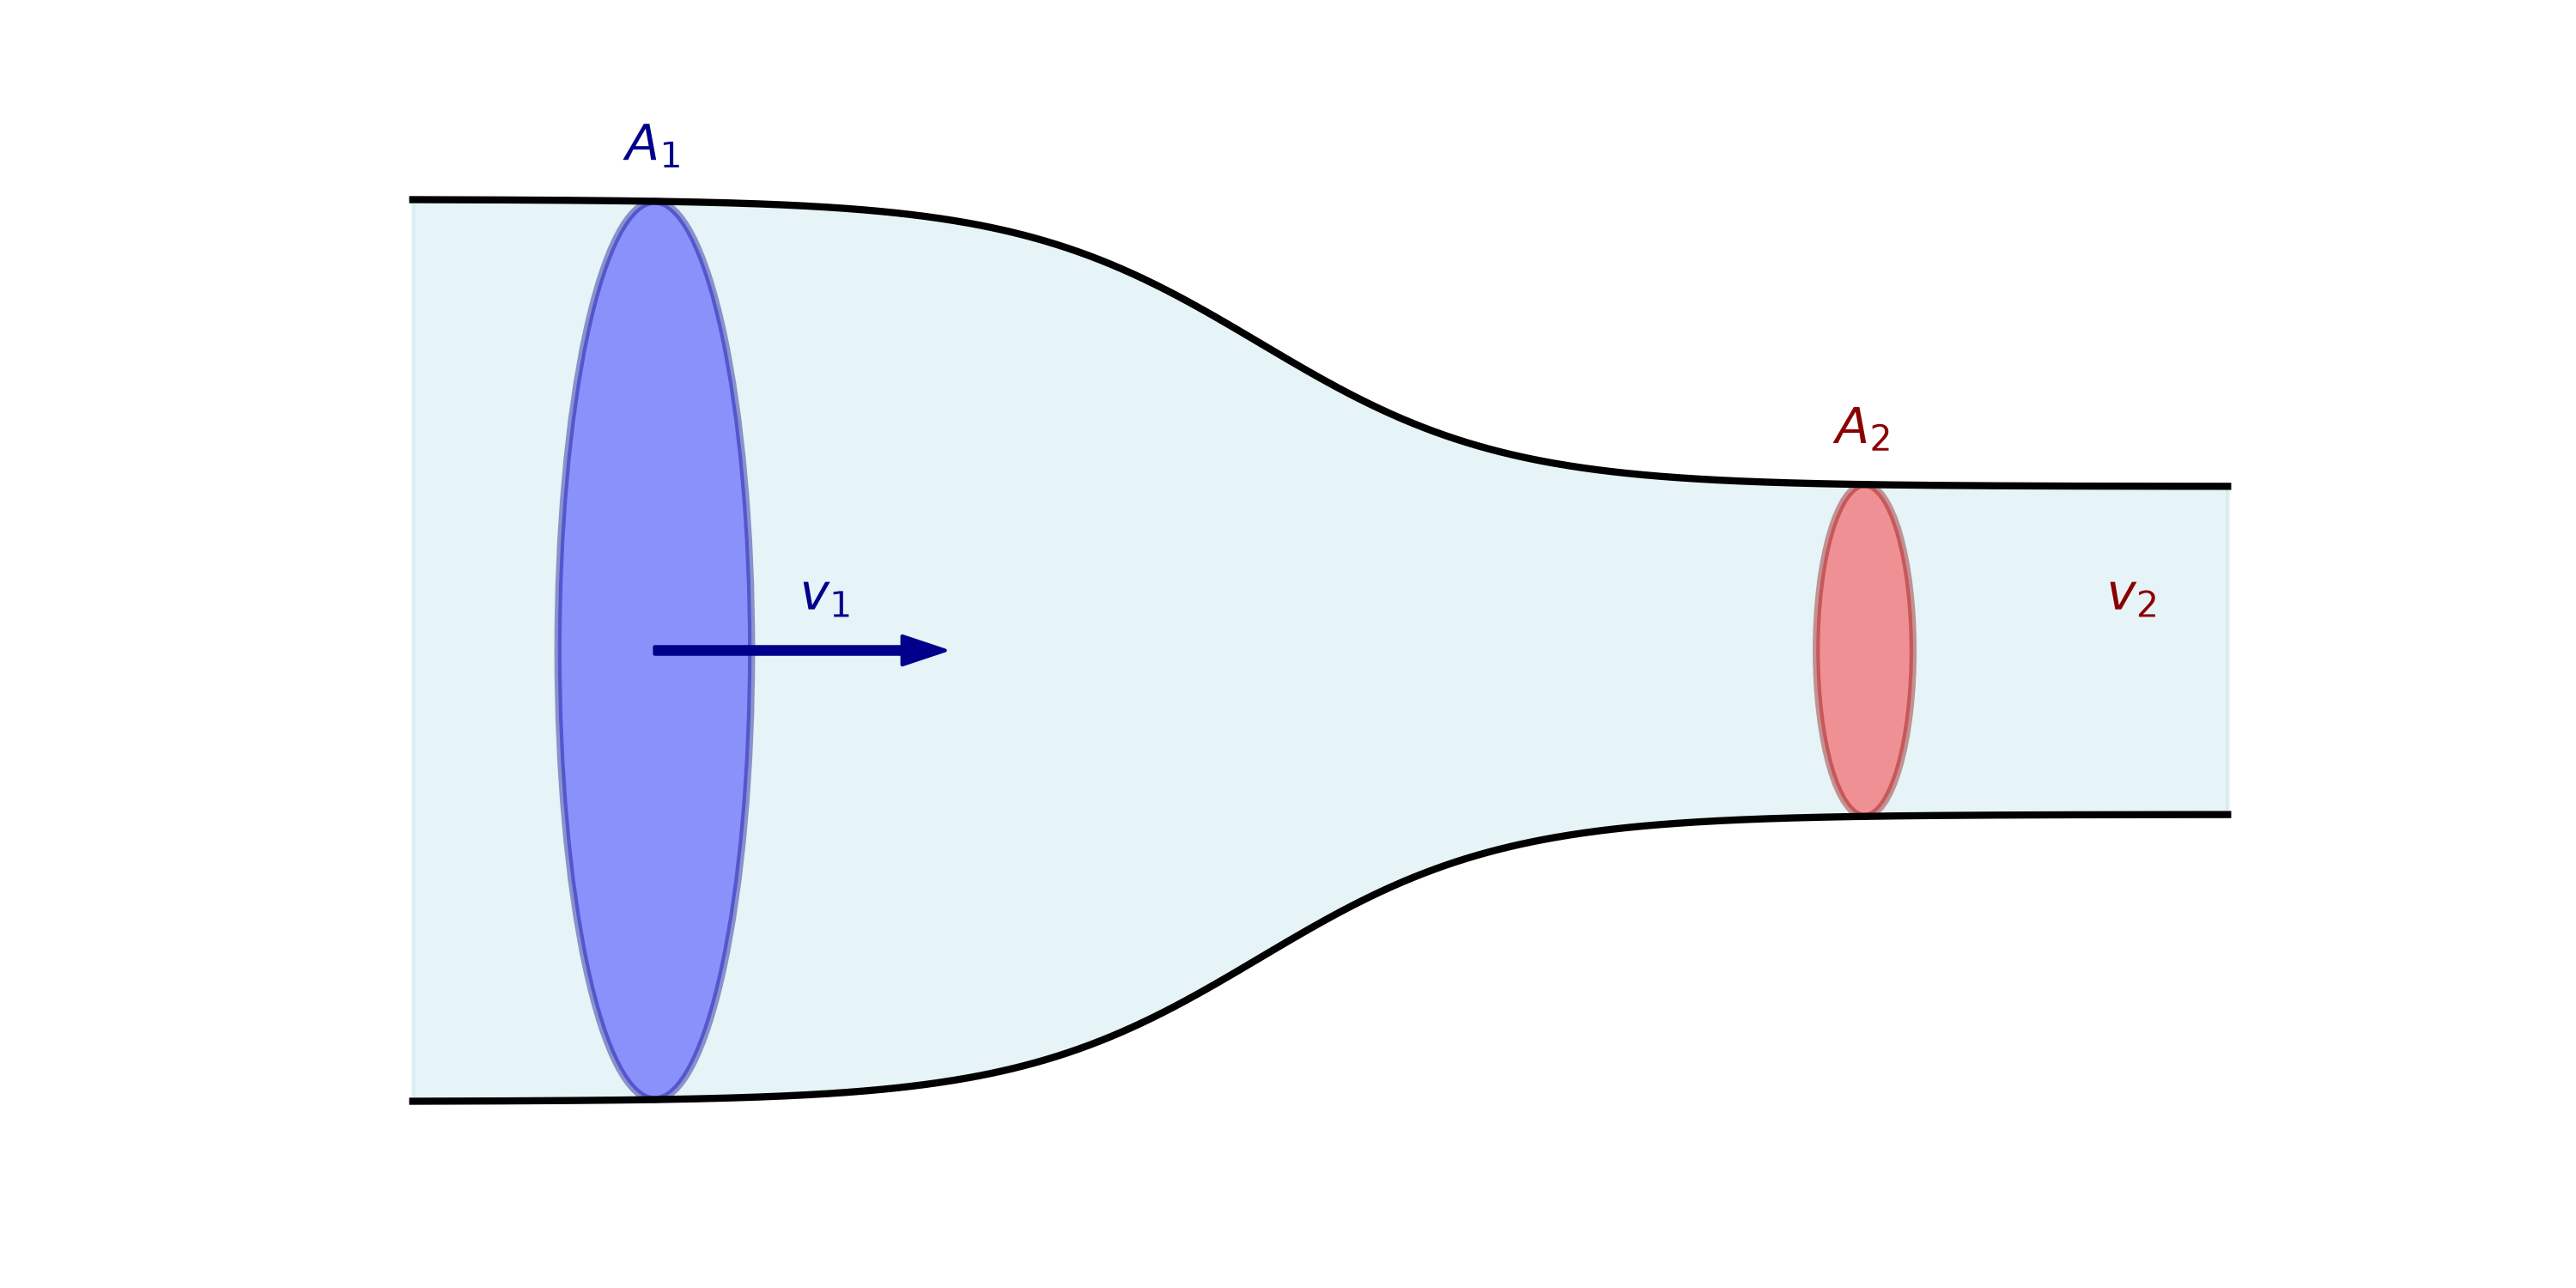
\includegraphics[width=0.5\linewidth]{img/tubo_di_flusso.png}
    \caption{Tubi di flusso e conservazione della massa}
    \label{fig:tubiDiFlusso}
\end{figure}

Poichè il tubo è sottile è possible trascurare la variazione di $\rho$ e $v$ sui punti delle basi.

Supponendo che il moto avvenga nella direzione $A_1 \longrightarrow A_2$, nell'intervallo di tempo $dt$ una quantità di fluido di volume $dV_1 = A_1v_1dt$ e massa $dm_1 = \rho_1dv_1$ entra nella porzione di sinistra, mentre una quantità di fluido di volume $dV_2 = A_2v_2dt$ e massa $dm_2 = \rho_2dv_2$ esce da destra.

Le porzioni del tubo di flusso ai tempo $t$ e $t + dt$ devono avere la stessa massa.

Inoltre essendo il moto stazionario, deve valere che la massa della parte comunque alla due porzioni non varia:
\begin{equation}
    dm_1 = dm_2 \implies \rho_1A_1v_1 = \rho_2A_2v_2 = \text{costante}
    \label{eq:equazioneDiContinuità}
\end{equation}
Nel caso di fluidi incompressibili, dove $\rho_1 = \rho_2$, allora:
\begin{equation}
    A_1v_1 = A_2v_2 = \text{costante}
\end{equation}

La quantità $Av$ è detta portata, essa corrisponde al volume di fluido che attraversa una sezione del tubo di flusso per unità di tempo.
L'invarianza della portata per fluidi incompressibili implica che, se un tubo di flusso si restringe la velocità aumenta e viceversa.

Le linee di flusso si addensano dove il tubo si restringe e la velocità è alta, mentre si diradano nelle zone ad alta velocità, come si vede in figura \ref{fig:lineeDiFlusso}.

\begin{figure}[h!]
    \centering
    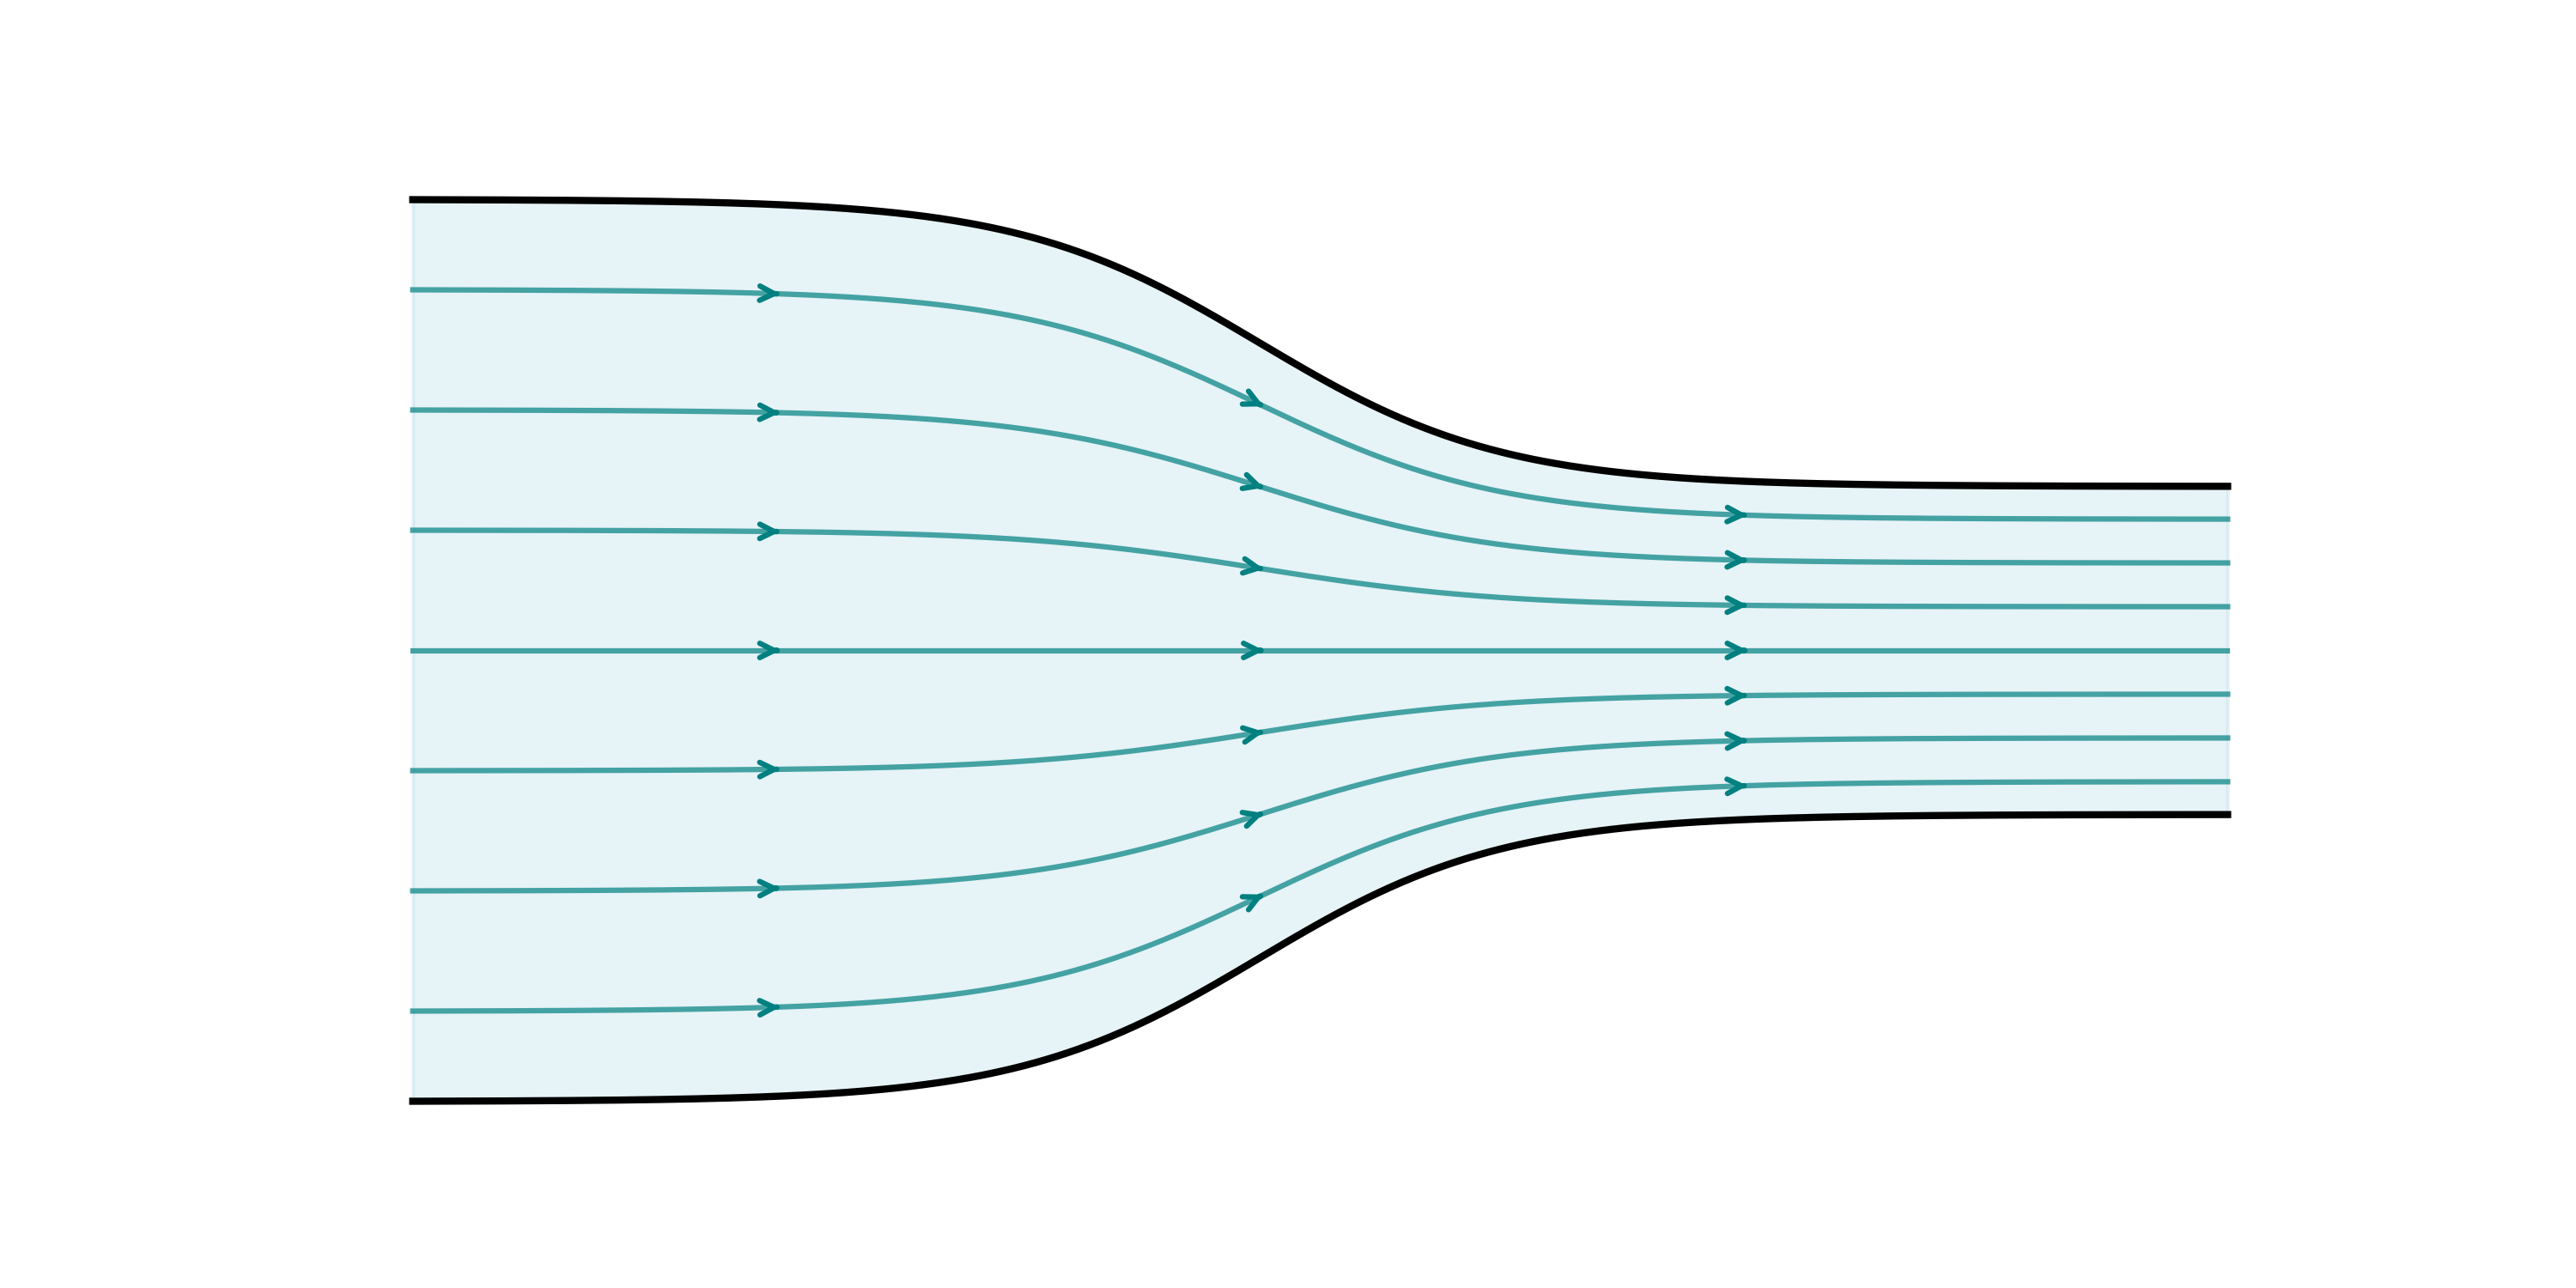
\includegraphics[width=0.6\linewidth]{img/linee_di_flusso.png}
    \caption{Linee di flusso}
    \label{fig:lineeDiFlusso}
\end{figure}

D'ora in avanti verranno trattati solo fluidi non viscosi, ciò è una approssimazione, ma permette comunque di descrivere le caratteristiche del moto di fluidi poso viscosi in alcuni particolari regimi, come quelli dei moto ad alta velocità in maniera adeguata.

\subsection{Teorema di Bernoulli}
Se si considera un fluido perfetto, con moto stazionario e irrotazionale, sul quale agisce solo la forza volumica di gravità, allora, rispetando tutte le precedenti condizioni, vale il Teorema di Bernoulli. 
Tale teorema è una semplice conseguenza del Teorema delle forze vive. 

\begin{theorem}
    Considerando un fluido perfetto, con moto stazionario e irrotazionale, sul quale agisce solo la forza volumica di gravità, allora lungo una linea di flusso vale che:
    \begin{equation}
        \frac{p}{\rho} + \frac{1}{2}v^2 + gh = costante
    \end{equation} 
\end{theorem}

\begin{proof}
    Considerando un tubo di flusso, supponendo che il fluido al suo interno si muova da sinistra a destra, allora le uniche forze che compiono lavoro sono la forza peso e le forza di pressione che agiscono sulle basi, in quanto quelle che agiscono sulla superficie laterale sono perpendicolari al moto, poichè in un fluido ideale non vi sono sforzi di taglio.

    \begin{figure}[h]
        \centering
        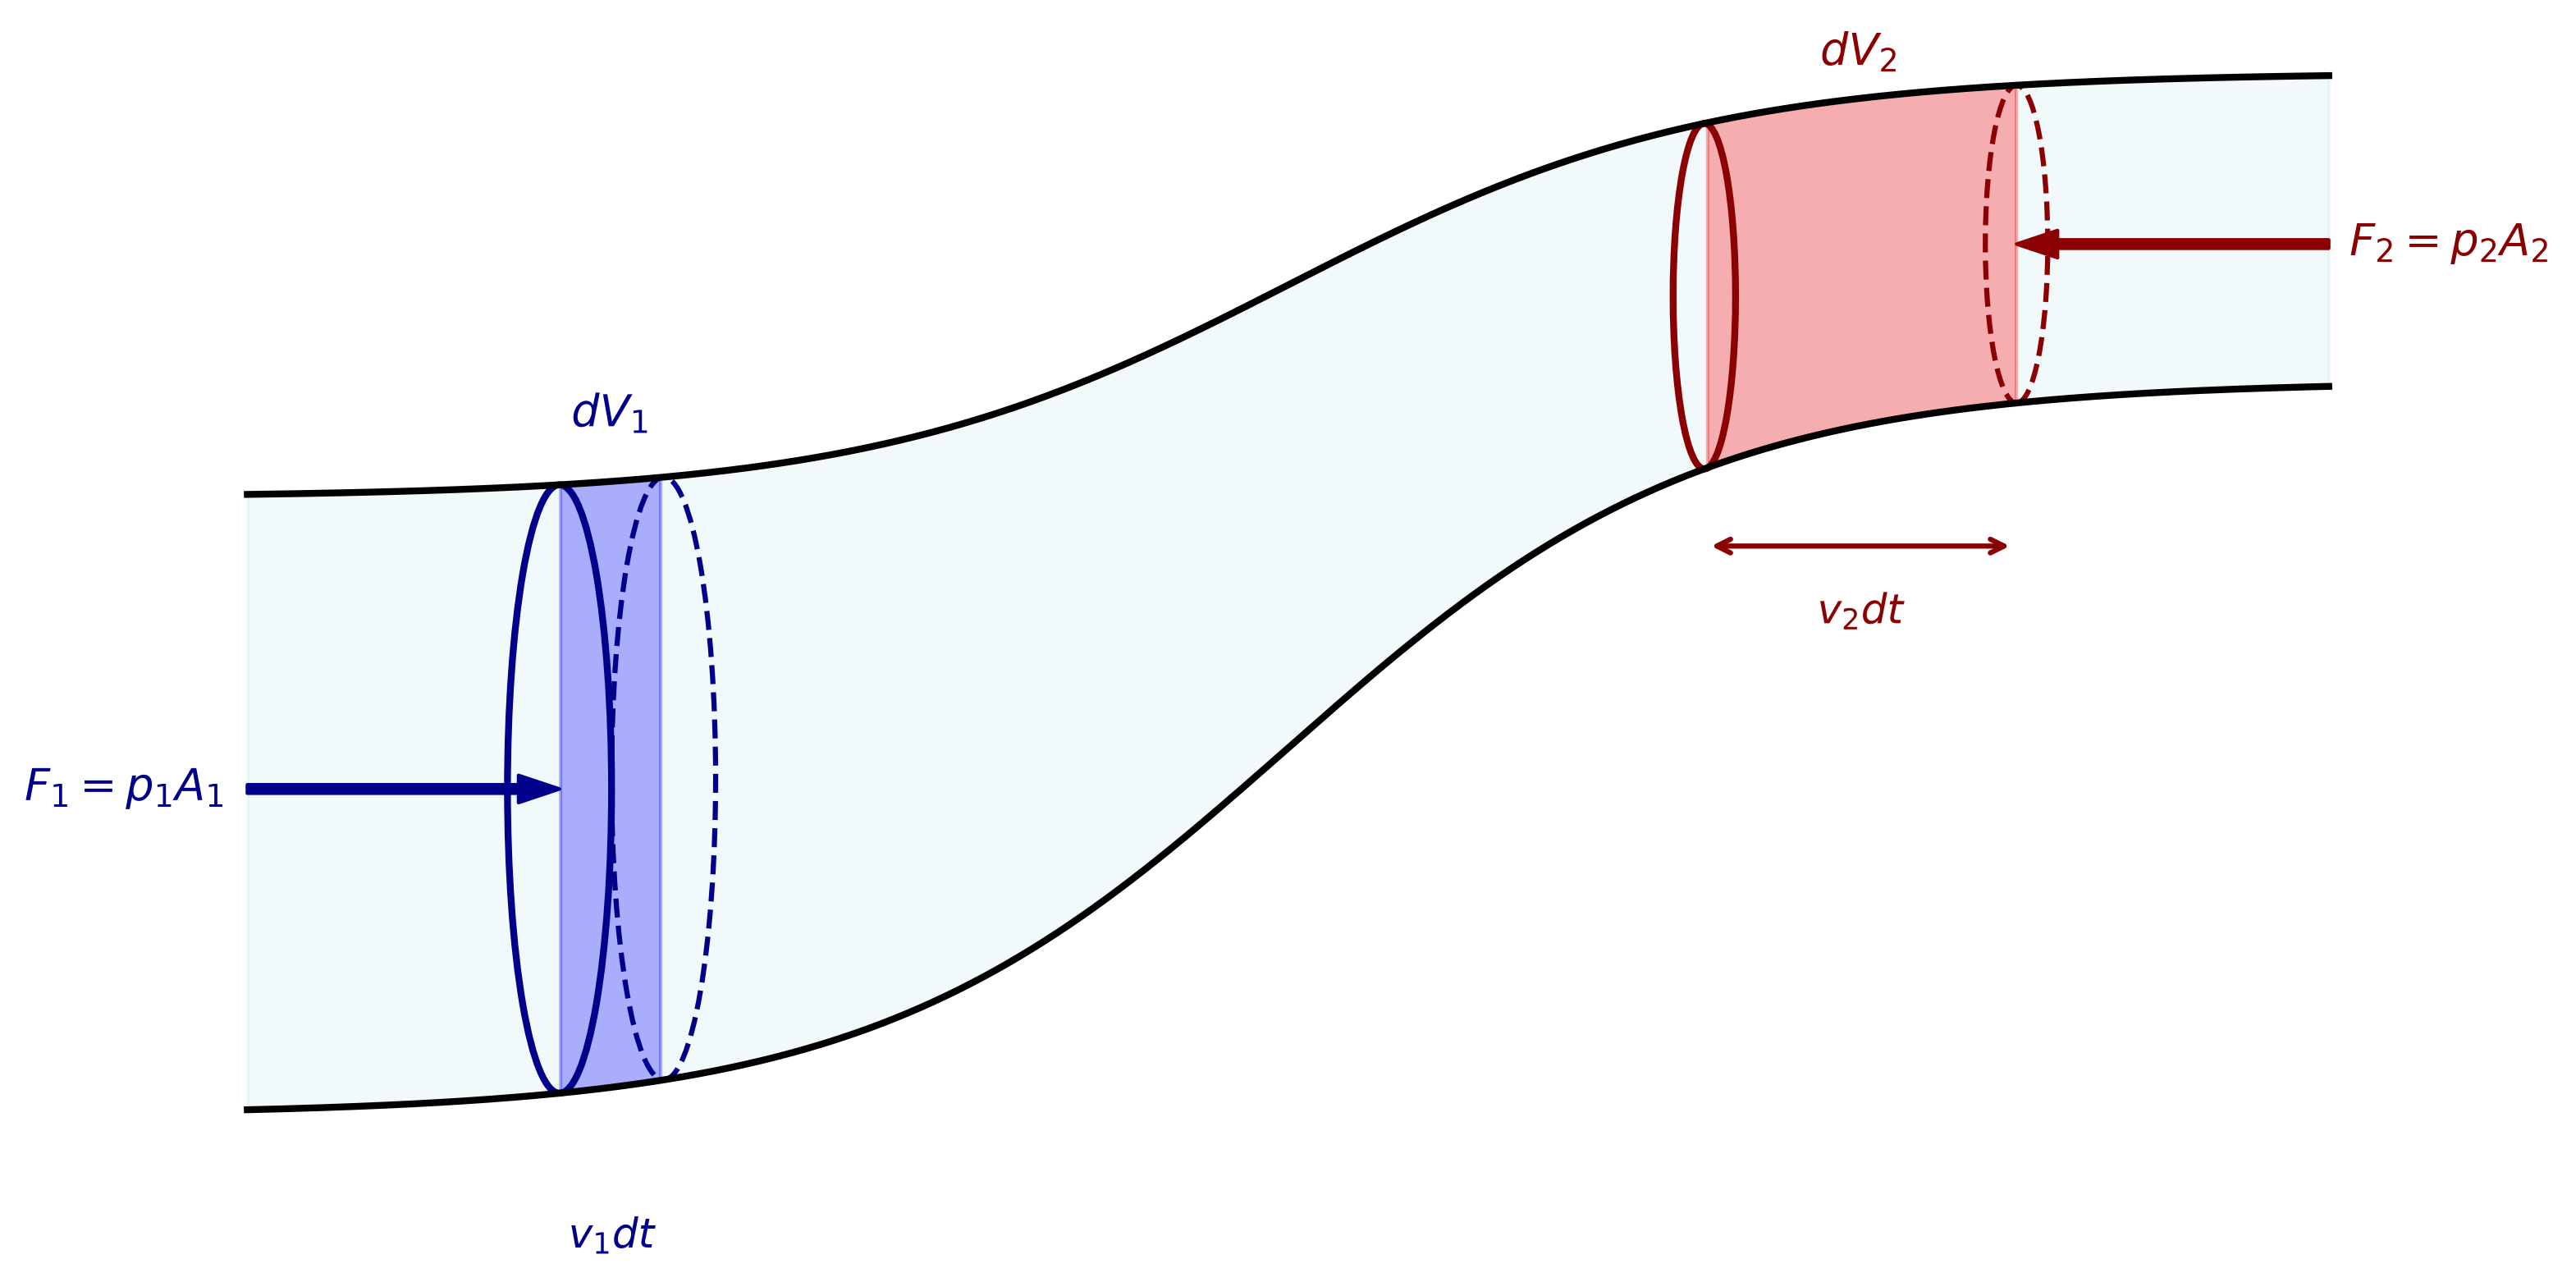
\includegraphics[width=0.75\linewidth]{img/teorema_bernoulli_vdt.png}
        \caption{Lavoro delle forze di pressione sul tubo di flusso}
        \label{fig:teoremaDiBernoulli}
    \end{figure}
    
    Vale quindi che:
    \begin{equation}
        F_1 = p_1A_1 \quad e \quad F_2 = p_2A_2
    \end{equation}
    Supponendo nuovamente che il tubo di flusso sia sottile e quindi la velocità del fluido sia costante sulle singola facce, il lavoro compiuto da $\vec{F}_1$ e da $\vec{F}_2$ in un tempo $dt$ vale:
    \begin{align}
        dL_p & = dL_1 + dL_2 \\
             & = F_1v_1dt - F_2v_2dt \\
             & = p_1A_1v_1dt - p_2A_2v_2dt \\
             & = p_1dV_1 - p_2dV_2 \\
             & = (p_1 - p_2)dV \\
             & = \frac{(p_1 - p_2)}{\rho}dm \\
    \end{align}
    I due volumi $dV_1$ e $dV_2$ sono uguali in quanto massa uguale e la densità $\rho$ è costante (fluido incompressibile).

    Per quanto riguarda il lavoro compiuto dalla forza esso è pari a meno la variaza di energia potenziale $dV_{peso}$. Essa si può calcolare denendo conto del fatto che esiste una parte comunque alle due porzioni di fluido corrispondenti a $t$ e $t + dt$, pertanto la variazione di energia potenziale della massa dm nella due configurazioni è:
    \begin{equation}
        \delta L_{peso} = -dV_{peso} = dmg(h_1 - h_2)
    \end{equation}
    Analogamente si calcola la variazione di energia cinetica, essendo il moto stazionario, il contributo a K della parte comune delle due porzioni di fluido non cambia nel tempo, pertanto:
    \begin{equation}
        dK = \frac{1}{2}dmv_2^2 - \frac{1}{2}dmv_1^2
    \end{equation}
    tale quantità deve essere pari al lavoro totale compiuto dalle forze di pressione e dalla forza peso, quindi vale:
    \begin{equation}
        dK = \frac{1}{2}dmv_2^2 - \frac{1}{2}dmv_1^2 = \frac{(p_1 - p_2)}{\rho}dm + dmg(h_1 - h_2)
    \end{equation}
    dividendo per $dm$ si ottiene:
    \begin{equation}
        \frac{p_1}{\rho} + \frac{1}{2}v_1^2 + gh_1 = \frac{p_2}{\rho} + \frac{1}{2}v_2^2 + gh_2 = costante
    \end{equation}
    pertanto si può concludere che lungo una linea di flusso deve valere:
    \begin{equation}
        \frac{p}{\rho} + \frac{1}{2}v^2 + gh = costante
    \end{equation}
    si è pertanto dimostrato il Teorema di Bernoulli.
\end{proof}
Dividendo per $g$ si ottiene la relazione:
\begin{equation}
    \frac{p}{g\rho} + \frac{1}{2}\frac{v^2}{g} + h = costante
\end{equation}
dove i 3 termini hanno una semplice interpretazione fisica, infatti:
\begin{itemize}
    \item $\frac{p}{\rho g}$ rappresenta l'altezza che una colonna di fluido deve avere affinchè la sua pressione sia p, detta \textit{altezza piezometrica}
    \item $\frac{1}{2}\frac{v^2}{g}$ rappresenta l'altezza da cui deve cadere un fluido affinche la velocità alla quota di arrivo sia $v$, ed è detta \textit{altezza cinetica}
    \item $h$ altezza effettiva 
\end{itemize}

\newpage

\subsection{Tubo di Venturi}
Il tubo di Venturi è un condotto orizzontale a sezione variabile, come in figura.

Indicando con $A_1$ la sezione nel tratto largo e con $A_2$ la sezione nella strozzatura. I tubi verticali aperti verso l'esterno servono a misurare le pressioni (e quindi le velocità) tramite una misure delle altezze delle colonne di liquido.

Supponendo che il fluido sia perfetto e non viscoso, allora vale il Teorema di Bernoulli:
\begin{equation}
    \frac{p_1}{g\rho} + \frac{1}{2}\frac{v_1^2}{g} + h_1 =\frac{p_2}{g\rho} + \frac{1}{2}\frac{v_2^2}{g} + h_2
\end{equation}
Poichè le sezioni si trovano alla stessa altezza $h_1 = h_2$, quindi vale che:
\begin{equation}
    \frac{p_1}{g\rho} + \frac{1}{2}\frac{v_1^2}{g} = \frac{p_2}{g\rho} + \frac{1}{2}\frac{v_2^2}{g}
\end{equation}
Inoltre conservandosi la portata segue che:
\begin{equation}
    A_1v_1 = A_2v_2 \implies v_2 \frac{A_1}{A_2}v_1 > v_1
\end{equation}
si vuole però definire $v_1$ in funzione di $h$.

Poichè la velocità è maggiore in $A_2$, la pressione è minore, tale effetto è detto appunto \textit{effetto venturi}, il che può apparire controintuitivo.

Dal Teorema di Bernoulli e dalla conservazione della portata si ricava che:
\begin{equation}
    p_1 - p_2 = \frac{1}{2}(v_2^2 - v_1^2) = \frac{1}{2}\rho v_1^2 \left(\left(\frac{A_1}{A_2}\right)^2 - 1\right)
\end{equation}
Siccome le altezze delle colonne di fluido in 1 e 2 sono pari a:
\begin{equation}
    h_1 = \frac{p_1}{\rho g} \quad e \quad h_2 = \frac{p_2}{\rho g}
\end{equation}
allora si ottiene:
\begin{equation}
    \Delta h = h_1 - h_2 = \frac{1}{2}\frac{v_1^2}{g}\left(\left(\frac{A_1}{A_2}\right)^2 - 1\right) \implies v_1^2 = 2g\Delta h\left(\frac{A_2^2}{A_1^2 - A_2^2}\right)
\end{equation}

% INSERIRE FIGURA VENTURI E PITOT

\subsection{Tubo di Pitot}
Il tubo di Pitot è un altro strumento per la misurazione della velocità di un fluido, che questa volta viene ottenuta misurando la pressione necessaria per fermare il fluido stesso.

Nella sua forma più semplice esso ha la forma di una L e viene parlazialmente immerso come in figura.

In questo modo il fluido che penetra nel tubo si arresta.

Se il rabo del tubo immerso è orizzontale, per il teorema di Bernoulli vale:
\begin{equation}
    \frac{p_{est}}{\rho g} + \frac{1}{2}\frac{v^2}{g} = \frac{p_{in}}{\rho g}
\end{equation} 
essendo il fluido fermo in corrispondenza di $p_{in}$.

Siccome vale, per la legge di Stevino, che:
\begin{equation}
    \Delta p = \rho g h \implies h = \frac{p_{in}}{\rho g} - \frac{p_{est}}{\rho g}
\end{equation}
allora si ottiene che:
\begin{equation}
    v = \sqrt{2gh}
\end{equation}
pertanto la misura di $h$ fornisce immediatamente il valore della velocità del fluido.

\section{Fluidi reali}
I fluidi reali sono viscosi e la presenza di sforzi di taglio complica di molto l'analisi del moto. 

Le caratteristiche del moto stesso dipendono molto dalla velocità.
A basse velocità, il è in così detto regime di flusso laminare, dove, i tubi di flusso infinitesimi in cui può essere scomposto il fluido, scorrono gli uni sugli altri con velocità diverse e sforzi di taglio reciproci, ma essi mantengono la loro individualità.

Aumentando la velocità, si raggiunge un valore critico, al di sopra del quale i tubi non sono più "impermeabili" e quindi inizano a mescolarsi e/o si formano vortici, tale comportamento corrisponde al regime turbolento.

\subsection{Viscosità}
È possibile dare una definizione di viscosità considerando un moto laminare semplice, ovvero il moto dell'acqua in un canale in pianura.

In questo caso la velocità degli strati d'acqua dipende solo dalla coordinata $z$, ma a causa delle forze d'attrito fra gli strati d'acqua, la velocità dell'acqua diminuisce via via che si scendo in profondità, e lo strato a diretto contatto con il fondale ha velocità nulla.

Sperimentalmente si osserva che, lo sforzo di taglio orizzontale è proporzionale alla derivata della velocità del fluido rispetto alla quota:
\begin{equation}
    T = \frac{dF_s}{ds} = \eta \frac{dv}{dz}
\end{equation}
dove il coefficiente $\eta$ è detto viscosità, essa dipende dalle caratteristiche che fluido.

\section{Portanza}
La portanza è la \textit{spinta aereodinamica} verso l'alto che permette agli aerei di volare. Essa ha una natura fisica diversa dalla spinta di Archimede.

Infatti, la portanza viene esercitata dall'aria solo se il corpo è in moto rispetto al fluido.

La portanza è un fenomeno complesso, quindi verranno fornite due spiegazioni qualitative del fenomeno basate sul III principio della dinamica e sul teorema di Bernoulli.

\subsection{Portanza tramite il III principio}
Poichè l'ala esercita una forza verso il basso sull'aria mentre questa le scorre attorno, allora per il III principio, l'aria deve esercitare una forza uguale e contraria sull'ala, ovvero la portanza.

È importante notare che la forza sul fluido non è prodotta solo dalla superficie inferiore dell'ala.

Tale spiegazione è corretta ma non da informazioni sul comportamento dell'aria intorno all'ala, nello specifico non mette in relazione la portanza con le differenza di pressione sopra e sotto l'ala.

\subsection{Portanza tramite il Teorema di Bernoulli}
Considerando un corpo che si muove in un fluido con velocità relativa $\vec{v}$, allora le interazioni fra il corpo e il fluido sono le stesse che ci sarebbero se il corpo fosse fermo e il fluido lo investisse con velocità $-\vec{v}$.

Considerando il profilo dell'ala di un aeroplano, allora le linee di flusso si adattano alla forma del profilo alare.

A causa dell'inclinazione e della forma dell'ala le linee di flusso si addensano nella parte superiore, come accadrebbe in una strozzatura, pertanto la velocità del fluido è maggiore nella parte superiore rispetto a quella inferiore.

Dal Teorema di Bernoulli segue che la pressione sia più bassa nella parte superiore, il risultato nello è una spinta verso l'alto.

Tale dimostrazione è una semplificazione drastica e non del tutto corretta, infatti solo in un fluido viscoso può esservi la portanza. Inoltre l'aumento di densità di linee di flusso al disopra dell'ala è spiegato in termini di una strozzatura dovuta alla forma non simmetria del profilo alare, ma in reatà non vi è nessun confinamento geometrico.

\section{Effetto Magnus}
L'effetto magnus è un fenomeno che si osserva quando un corpo si muove in un fluido con moto roto-traslatorio. A causa della presenza del moto rotatorio, il corpo devia dalla traiettoria che avrebbe in assenza di tale moto.

L'effetto è tanto più marcato quanto più alta è la velocità di rotazione.

\begin{figure}[h]
    \centering
    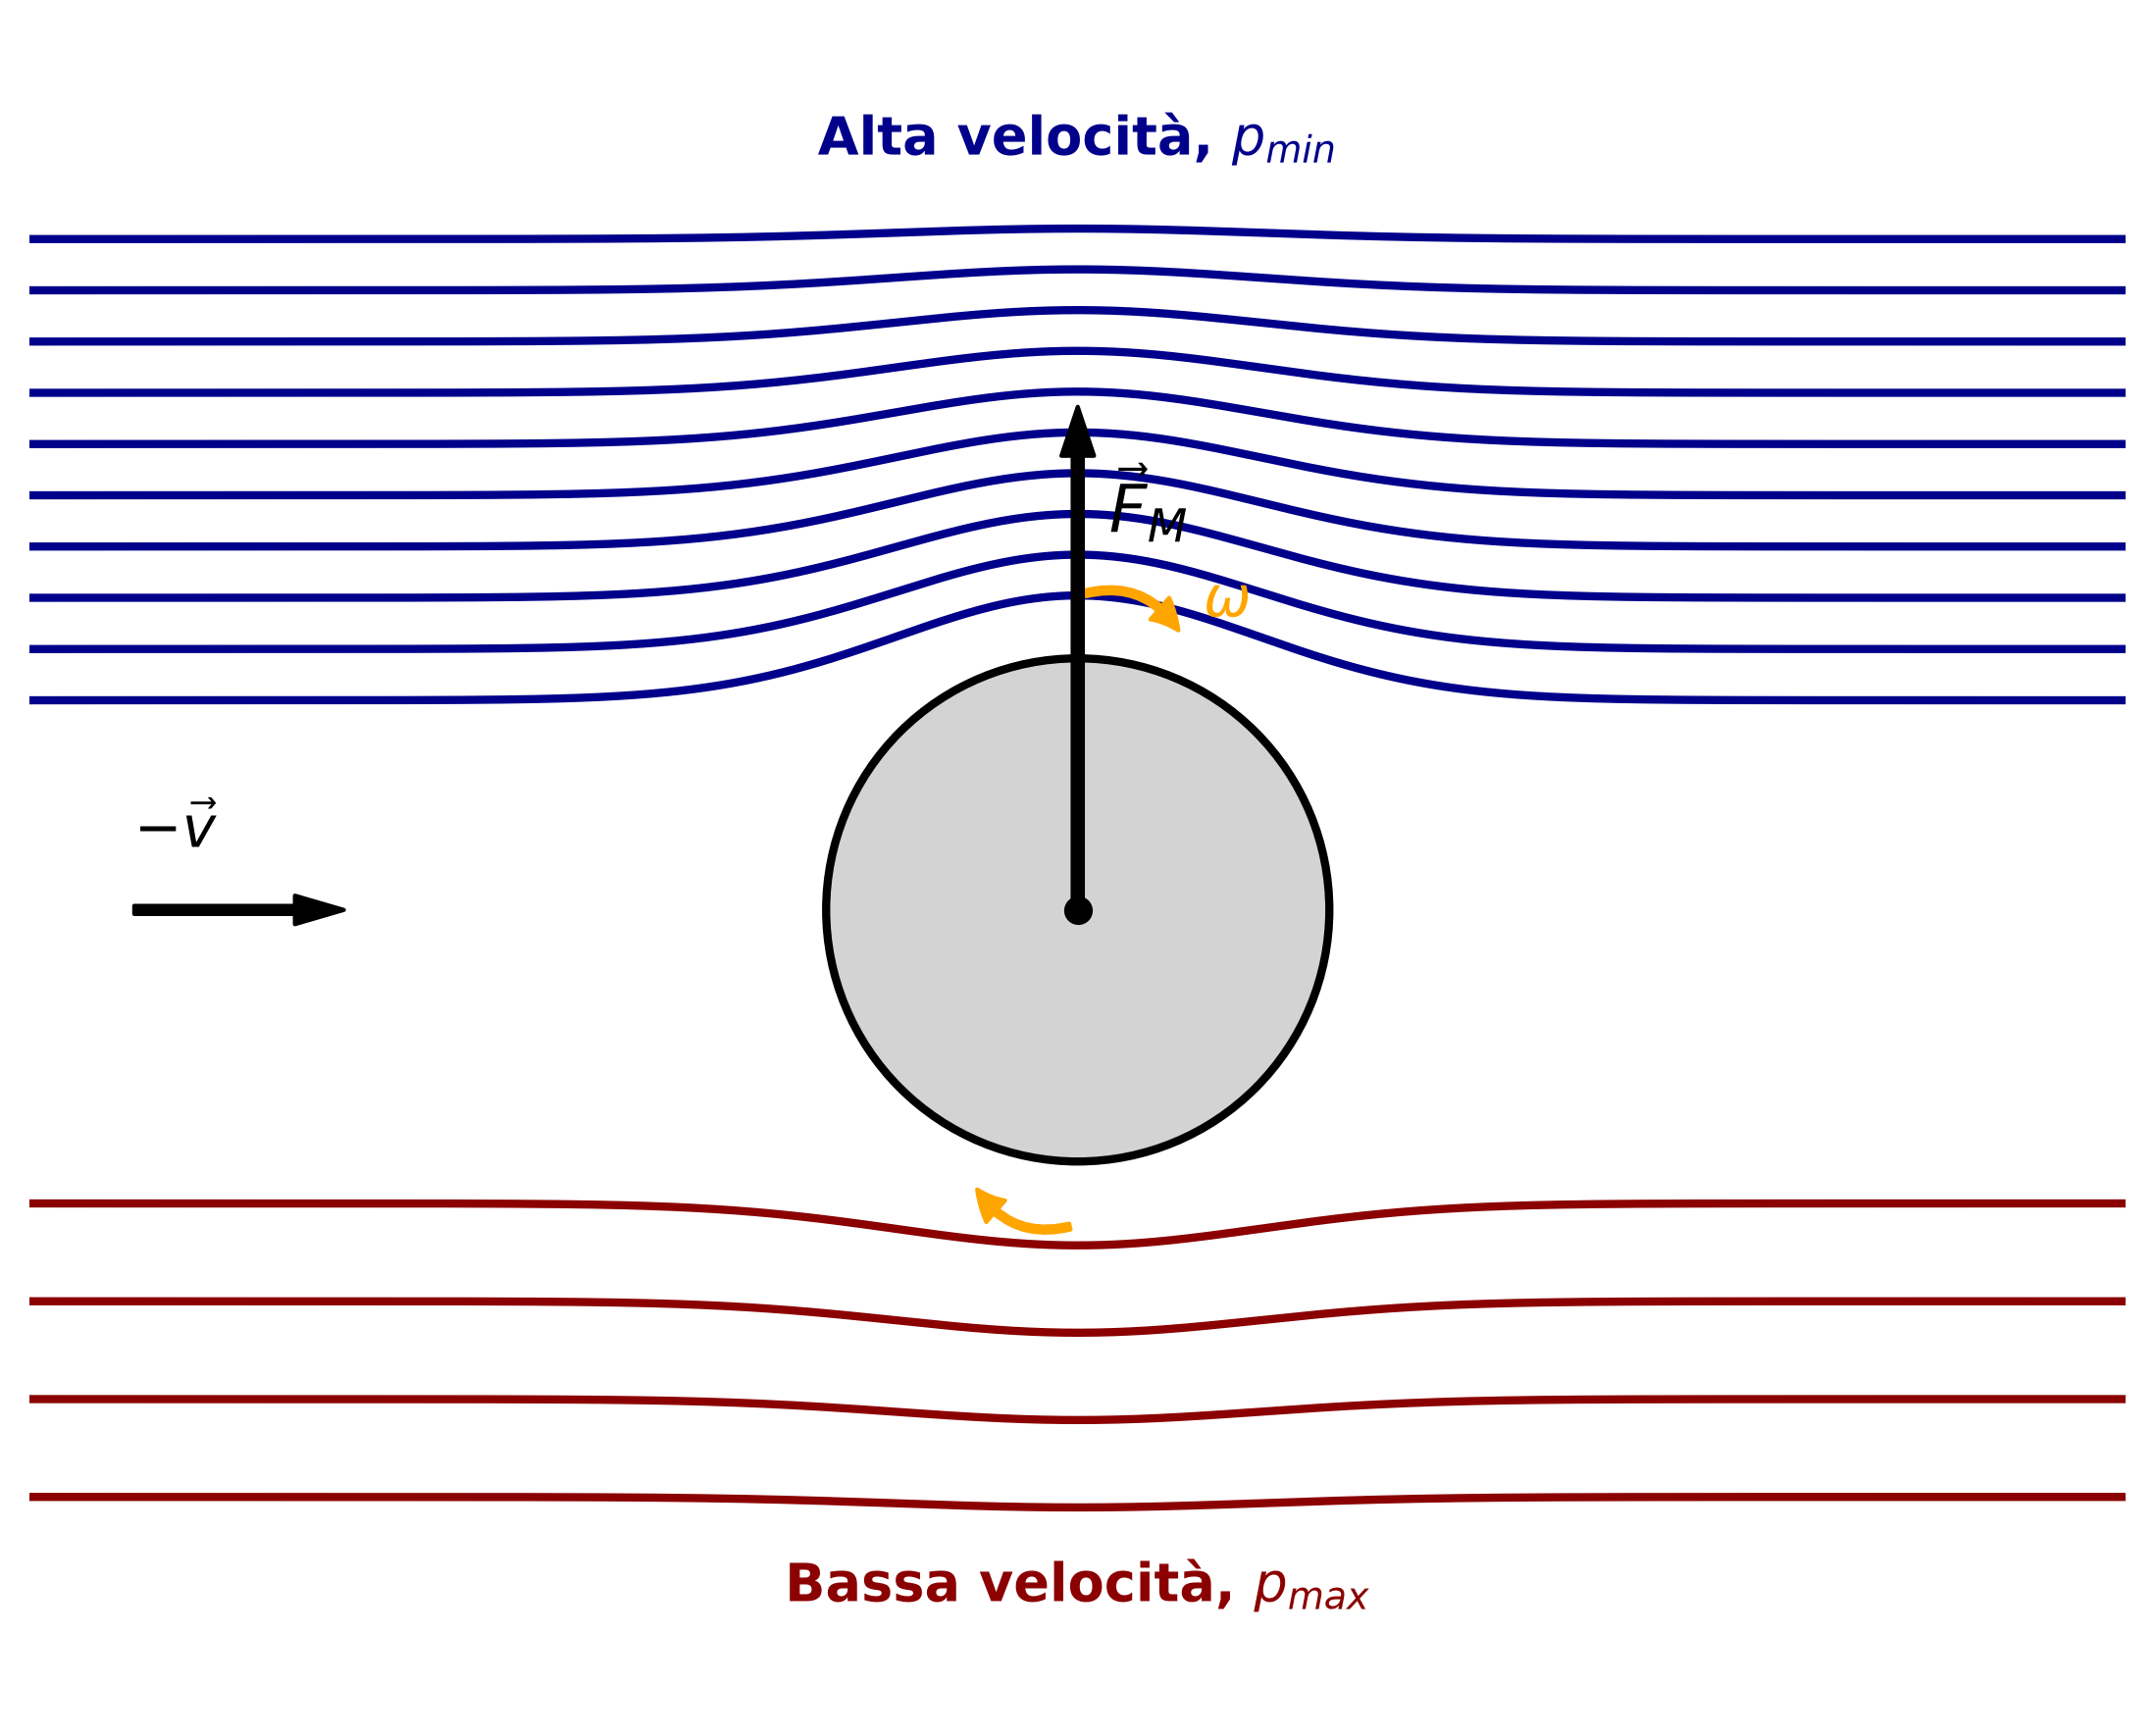
\includegraphics[width=0.7\linewidth]{img/effetto_magnus.png}
    \caption{Rappresentazione dell'effetto Magnus}
    \label{fig:effettoMagnus}
\end{figure}

La spiegazione di questo fenomeno presenza diverse analogia con quella della portanza, infatti se la velocità del centro di massa del corpo rispetto al fluido è $\vec{v}$, allora è possibile considerare un sistema equivalente in cui il corpo ha solo moto rotatorio e il fluido si muove con velocità $-\vec{v}$ rispetto ad esso.

Sopponendo che il corpo sia di forma sferica, abbia un moto rotatorio in senso orario e che il fluido si muova verso destra, allora è possibile immaginare che il corpo in rotazione trascini con se lo strato di fluido a contatto con esso e che questo strato trascini con se lo stratto vicino e così via.

Pertanto nella parte "al di sopra" del corpo, l'effetto del trascinamento tende ad aumentare la velocità del fluido, mentre nella parte inferiore l'effetto è opposto.

Di conseguenza, le linee di flusso sono più dense nella parte superiore e più rarefatte nella parte inferiore.

Per il Teorema di Bernoulli, la pressione è inferiore nella regione sopra il corpo, da cui segue che vi è una forza con direzione verso la zona di addensamente delle linee di flusso, e con verso positivo.   


\chapter{Onde}
Le onde si dividono in 3 tipologie:
\begin{itemize}
    \item Onde meccaniche
    \item Onde elettromagnetiche
    \item Onde gravitazionali
\end{itemize}

\section{Onde meccaniche}
Le onde meccaniche rappresentano una perturbazione di una proprietà fisica (rispetto all'equilibrio) che si propaga in un mezzo materiale, è importante notare che le onde meccaniche non rappresentano un trasferimento di materiale ma solo di energia e quantità di moto.

Vi sono 2 tipologie di onde meccaniche:
\begin{itemize}
    \item Onde trasversali nelle quali lo spostamento degli elementi del corpo soggetto alla perturbazione è perpendicolare alla direzione di propagazione. Questo tipo di onde può propagarsi solo nei solidi.
    \item Onde longitudinali nelle quali lo spostamento degli elementi del corpo soggetto alla perturbazione è parallelo alla direzione di propagazione. Al contrario delle onde trasversali, queste si possono propagare in ogni mezzo materiale.
\end{itemize}
Supponendo che:
\begin{itemize}
    \item la categoria di onde di interesse soddisfi il principio di sovrapposizione, allora tali onde devono essere una soluzione di una equazione differenziale alle derivate parziali.
    \item la forma delle onde si propaga inalterata nello spazio
\end{itemize}

\subsection{Onde trasversali}
Definendo come $\xi$ la funzione scalare che descrive lo spostamento dell'elemento d'onda in x all'istante t rispetto alla posizione di equilibrio, allora per le supposizioni precedenti deve valere:
\begin{equation}
    \xi(x, t = 0) = f(x)
\end{equation}

Se si studiano onde progessive, ovvero onde che si muovono con velocità positiva (rispetto agl'assi scelti), vale, per costruzione di $\xi$ stesso:
\begin{align}
    x, t &\longleftrightarrow x - vt, \quad t = 0 \\
    \xi(x, t) &= \xi(x - vt, 0) \\
              &= f(x - vt)
\end{align}
Mentre per le onde regressive (onde che si muovono con velocitò negativa rispetto agl'assi scelti), vale:
\begin{align}
    x, t &\longleftrightarrow x + vt, \quad t = 0 \\
    \xi(x, t) &= \xi(x + vt, 0) \\
              &= g(x + vt)
\end{align}

\begin{theorem}[Equazione di d'Alembert]
L'equazione di d'Alembert, detta anche equazione delle onde, è l'equazione
differenziale alle derivate parziali che definisce la categoria di onde che
rispettano le supposizioni precedentemente fatte:
\begin{equation}
    \frac{\partial^2 \xi}{\partial x^2} = \frac{1}{v^2} \frac{\partial^2 \xi}{\partial t^2}
\end{equation}
ove $v$ è una costante che equivale alla velocità di propagazione dell'onda.
\end{theorem}

\begin{proof}
Consideriamo una funzione d'onda della forma
\begin{equation}
    \xi(x, t) = f(x - vt).
\end{equation}
Introducendo la variabile ausiliaria
\begin{equation}
    w(x, t) = x - vt,
\end{equation}
si ha $\xi(x, t) = f(w(x, t))$. Derivando parzialmente $\xi$ rispetto ad $x$:
\begin{align}
    \pdv{\xi}{x} &= \dv{f}{w} \cdot \pdv{w}{x}
                  = \dv{f}{w} \cdot 1
                  = \dv{f}{w}.
\end{align}
Applicando nuovamente l'operatore $\pdv{}{x}$:
\begin{align}
    \pdv[2]{\xi}{x}
        &= \pdv{x}\!\left(\dv{f}{w}\right)
         = \dv[2]{f}{w} \cdot \pdv{w}{x}
         = \dv[2]{f}{w}.
\end{align}
Derivando invece rispetto al tempo, e usando $\pdv{w}{t} = -v$:
\begin{align}
    \pdv{\xi}{t}
        &= \dv{f}{w} \cdot \pdv{w}{t}
         = -v\dv{f}{w}.
\end{align}
Derivando una seconda volta rispetto al tempo:
\begin{align}
    \pdv[2]{\xi}{t}
        &= \pdv{t}\!\left(-v\dv{f}{w}\right)
         = -v\dv[2]{f}{w} \cdot \pdv{w}{t}
         = -v\dv[2]{f}{w} \cdot (-v)
         = v^2\dv[2]{f}{w}.
\end{align}
Confrontando le due derivate seconde si ottiene
\begin{equation}
    \pdv[2]{\xi}{x} = \dv[2]{f}{w} = \frac{1}{v^2}v^2\dv[2]{f}{w}
    = \frac{1}{v^2}\pdv[2]{\xi}{t},
\end{equation}
che è proprio l'equazione di d'Alambert. Poiché l'equazione è lineare e le
onde rispettano il principio di sovrapposizione, la soluzione generale è
\begin{equation}
    \xi(x, t) = f(x - vt) + g(x + vt),
\end{equation}
dove $f$ e $g$ sono funzioni arbitrarie che rappresentano rispettivamente
un'onda che si muove verso destra e una verso sinistra.
\end{proof}

Ciò si può generalizzare per il caso tridimensionale, introducendo l'operatore \textit{Laplaciano}, definito come segue:
\begin{align}
    \nabla^2 & = \vec{\nabla} \cdot \vec{\nabla} \\
             & = \pdv[2]{}{x} + \pdv[2]{}{y} + \pdv[2]{}{z} 
\end{align}
Si mostra quindi che l'equazione di d'Alambert definendo $\xi$ come segue
\begin{equation}
    \xi(x, y, z, t)
\end{equation}
allora si ottiene:
\begin{equation}
    \pdv[2]{}{x} + \pdv[2]{}{y} + \pdv[2]{}{z} = \frac{1}{v^2} \pdv[2]{\xi}{t}
\end{equation}
applicando il laplaciano a $\xi$ si ottiene:
\begin{equation}
    \nabla^2 \xi = \frac{1}{v^2} \pdv[2]{\xi}{t}
\end{equation} 

\subsection{Onde piane}
Le onde piane solo soluzioni particolari dell'equazione di d'Alambert, sono descritte da:
\begin{align}
    \xi(\vec{r}, t) & = f(\hat{u}_n \cdot \vec{r} \pm vt) \\
                    & = f(xu_{n_x} + yu_{n_y} + zu_{n_z} \pm vt)
\end{align}
\begin{proof}
    Definendo una funzione ausiliaria come segue:
    \begin{align}
        w(\vec{r}, t) & = \hat{u}_n \cdot \vec{r} \pm vt \\
                      & = xu_{n_x} + yu_{n_y} + zu_{n_z} \pm vt
    \end{align}
    Derivando parzialmente segue che:
    \begin{align}
        \pdv{\xi}{x} = \dv{f}{w} \cdot \pdv{w}{x} = \hat{u}_{n_x} \cdot \dv{f}{w}
    \end{align}
    derivando nuovamente si ottiene:
    \begin{equation}
        \pdv[2]{\xi}{x} = \hat{u}_{n_x}^2 \dv[2]{f}{w}
    \end{equation}
    ciò vale anche per le altre variabili spaziali.
    
    Derivando quindi rispetto al tempo si ottiene:
    \begin{equation}
        \pdv{\xi}{t} = \pm v \dv{f}{w}
    \end{equation}
    derivando nuovamente si ottiene:
    \begin{equation}
        \pdv[2]{\xi}{t} = v^2 \dv[2]{f}{w}        
    \end{equation}
    segue quindi che:
    \begin{align}
        \pdv[2]{\xi}{x} + \pdv[2]{\xi}{y} + \pdv[2]{\xi}{z} & = (\hat{u}_{n_x}^2 + \hat{u}_{n_y}^2 + \hat{u}_{n_z}^2) \dv[2]{f}{w} = \frac{1}{v^2}\pdv[2]{\xi}{w} \\
        \nabla^2 \xi & = \dv[2]{f}{w} = \frac{1}{v^2} \pdv[2]{\xi}{w}
    \end{align}
\end{proof}
Tali onde sono dette onde piane, poiché il valore della perturbazione, per punti su piani perpendicolari a $\hat{u}_n$ è costante, infatti il valore:
\begin{equation}
    \hat{u}_n \cdot \vec{r} = costante
\end{equation}
per $\vec{r}$ appartententi al piano perpendicolare a $\hat{u}_n$

\subsubsection{Onde piane sinusoidali}
Le onde piane sinusoidali sono descritte dalla Formula \ref{eq:ondePianeSinusoidali}, ed esse hanno importanti applicazioni, come per esempio nel Teorema di Fourier.
\begin{equation}
    \xi(\vec{r}, t) = A\cos(\vec{k} \cdot \vec{r} \pm \omega t + \delta_0)
    \label{eq:ondePianeSinusoidali}
\end{equation}
nella quale:
\begin{itemize}
    \item $\vec{k}$ rappresenta il vattore d'onda, ovvero il vettore che rappresenta la direzione dell'onda.
    \item $A$ rappresenta l'ampiezza massima dell'onda.
    \item $\omega$ rappresenta la pulsazione.
    \item $\delta_0$ rappresenta la fase.
\end{itemize}
La forma presente nella formula \ref{eq:ondePianeSinusoidali} è equivalente alla seguente:
\begin{equation}
    \xi(\vec{r}, t) = A\cos(\vec{k}(\hat{u}_k \cdot \vec{r} \pm \frac{\omega}{k} t ) + \delta_0)    
\end{equation}
dalla quale si può ricavare la velocità di propagazione, anche detta velocità di fase nel caso di onde sinusoidale, tramite la seguente formula:
\begin{equation}
    v = \frac{\omega}{k}
\end{equation}
Nell'ipotesi dove $\hat{u}_k \equiv \hat{x}$ e $\delta_0 = 0$, allora:
\begin{equation}
    \xi(x, t) = A\cos(kx - \omega t)
\end{equation}
da questa funzione fissando la coordinata temporale o la coordinata spaziale si trovano rispettivamente il periodo spaziale e il periodo temporale, presenti in figura \ref{fig:periodiTemporaliESpazialiOndePiane}, e descritti dalle formule \ref{eq:lunghezzaOnda} e \ref{eq:periodoTemporale}.
\begin{figure}[h]
    \centering
    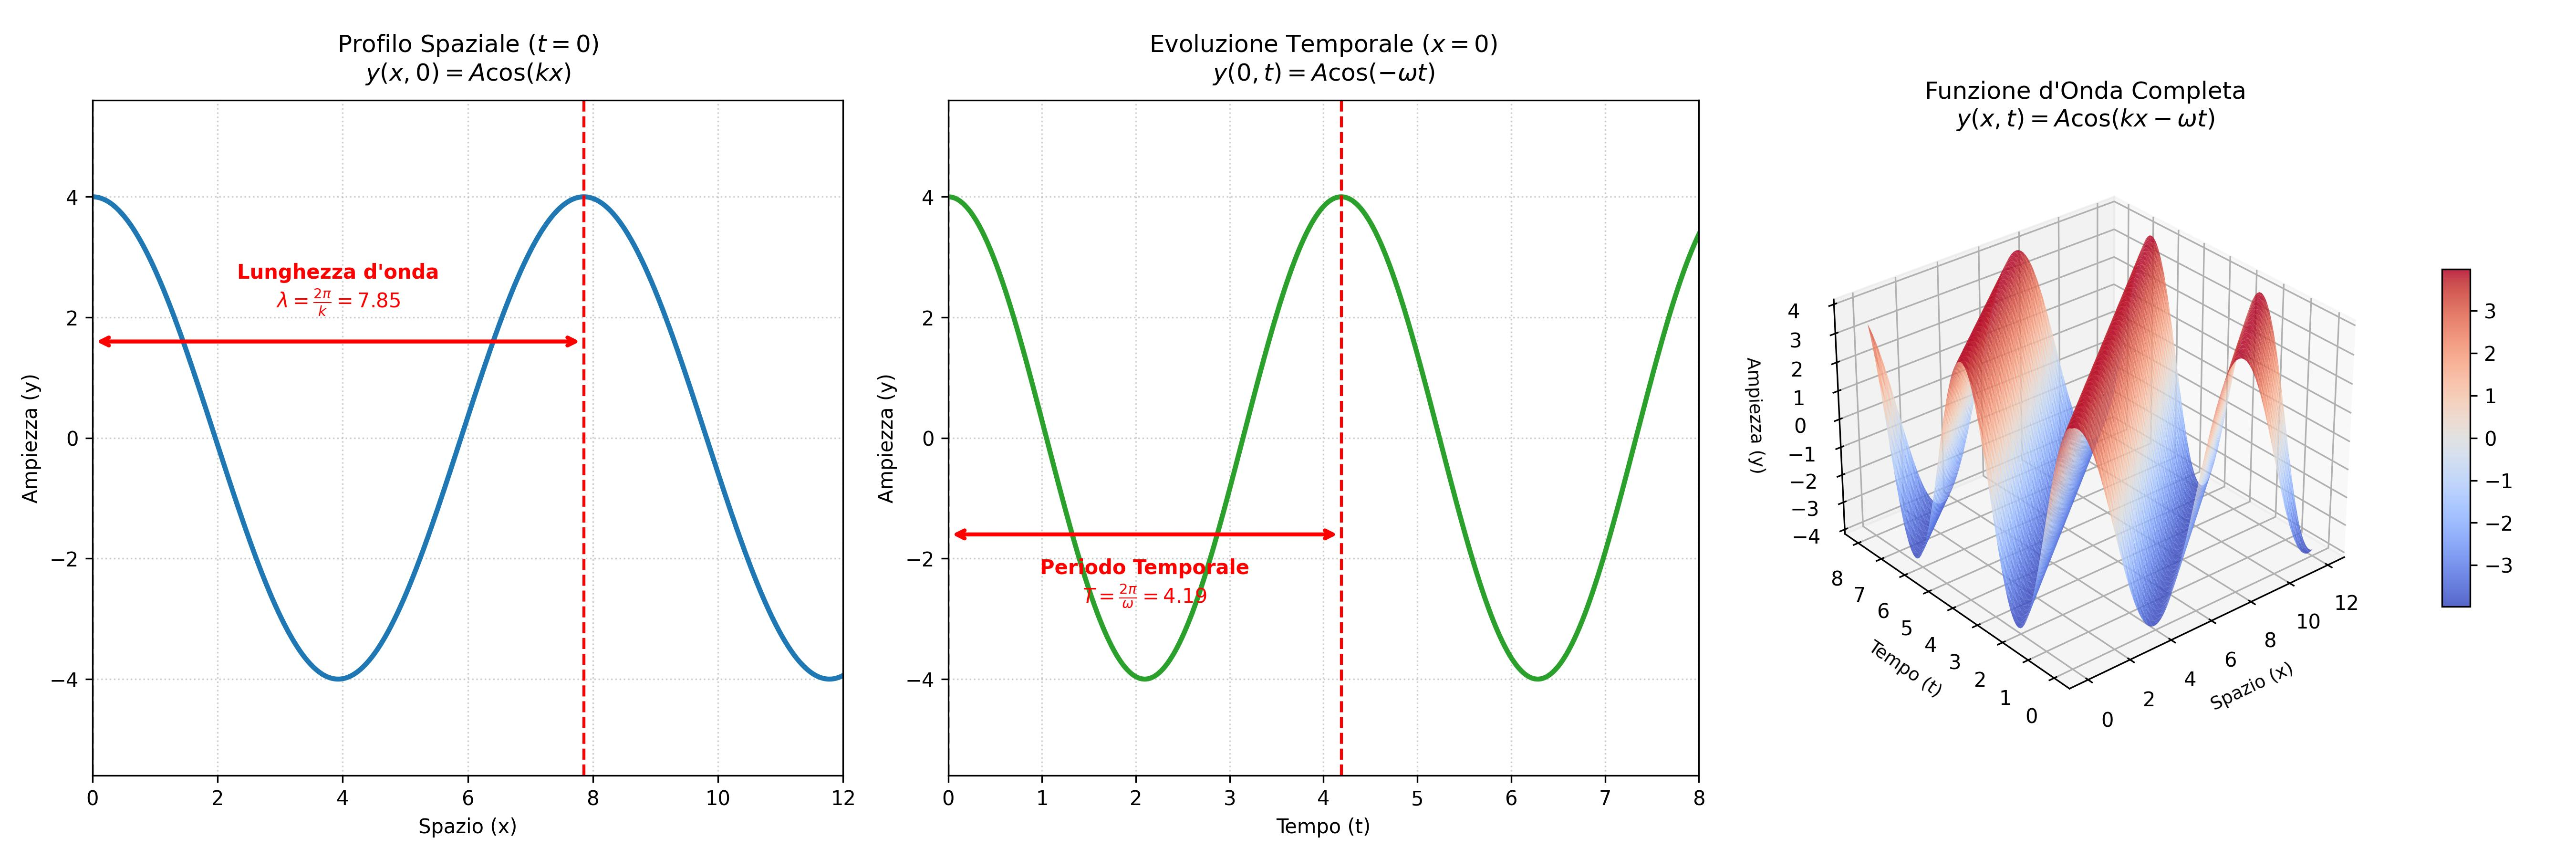
\includegraphics[width=1\linewidth]{img/periodiTemporaliESpazialiOndePiane.jpg}
    \caption{Andamento spaziale e temporale di una generica onda piana sinusoidale}
    \label{fig:periodiTemporaliESpazialiOndePiane}
\end{figure} 

\begin{equation}
    \lambda = \frac{2\pi}{k}
    \label{eq:lunghezzaOnda}
\end{equation}
\begin{equation}
    T = \frac{2\pi}{\omega}
    \label{eq:periodoTemporale}
\end{equation}

da ciò segue che:
\begin{equation}
    v = \frac{\omega}{k} = \frac{\lambda}{T}
\end{equation}

\section{Formalismo complesso per le onde monocromatiche}
Per rappresentare un'onda monocromatica è possibile studiare la parte reale di funzioni complesse, infatti:
\begin{align}
    f & = A\cos(\vec{k}\vec{r} \pm \omega t + \delta_0) \\
      & = A\cos(\alpha); \quad \alpha = \vec{k}\vec{r} \pm \omega t + \delta_0 \\
      & = \Re{Ae^{i\alpha}}
\end{align}
allora, definendo:
\begin{equation}
    z = Ae^{i\alpha}
\end{equation}
è possibile studiare le sovrapposizioni di onde.

\subsection{Sovrapposizione di onde monocromatiche}
Siano $f_1$ e $f_2$ due generiche onde monocromatiche, con direzione di propagazione lungo $x$, ma con fase differente, definite come segue:
\begin{equation}
    f_1 = A_1\cos(kx \pm \omega t)
\end{equation}
\begin{equation}
    f_2 = A_2\cos(kx \pm \omega t + \delta)
\end{equation}
Allora queste funzioni sono eqiuvalenti a:
\begin{equation}
    \begin{cases}
        f_1 = \Re{z_1}; z_1 = A_1e^{i\alpha} \\
        f_2 = \Re{z_2}; z_2 = A_2e^{i\alpha}
    \end{cases}
\end{equation}

\begin{figure}[h]
    \centering
    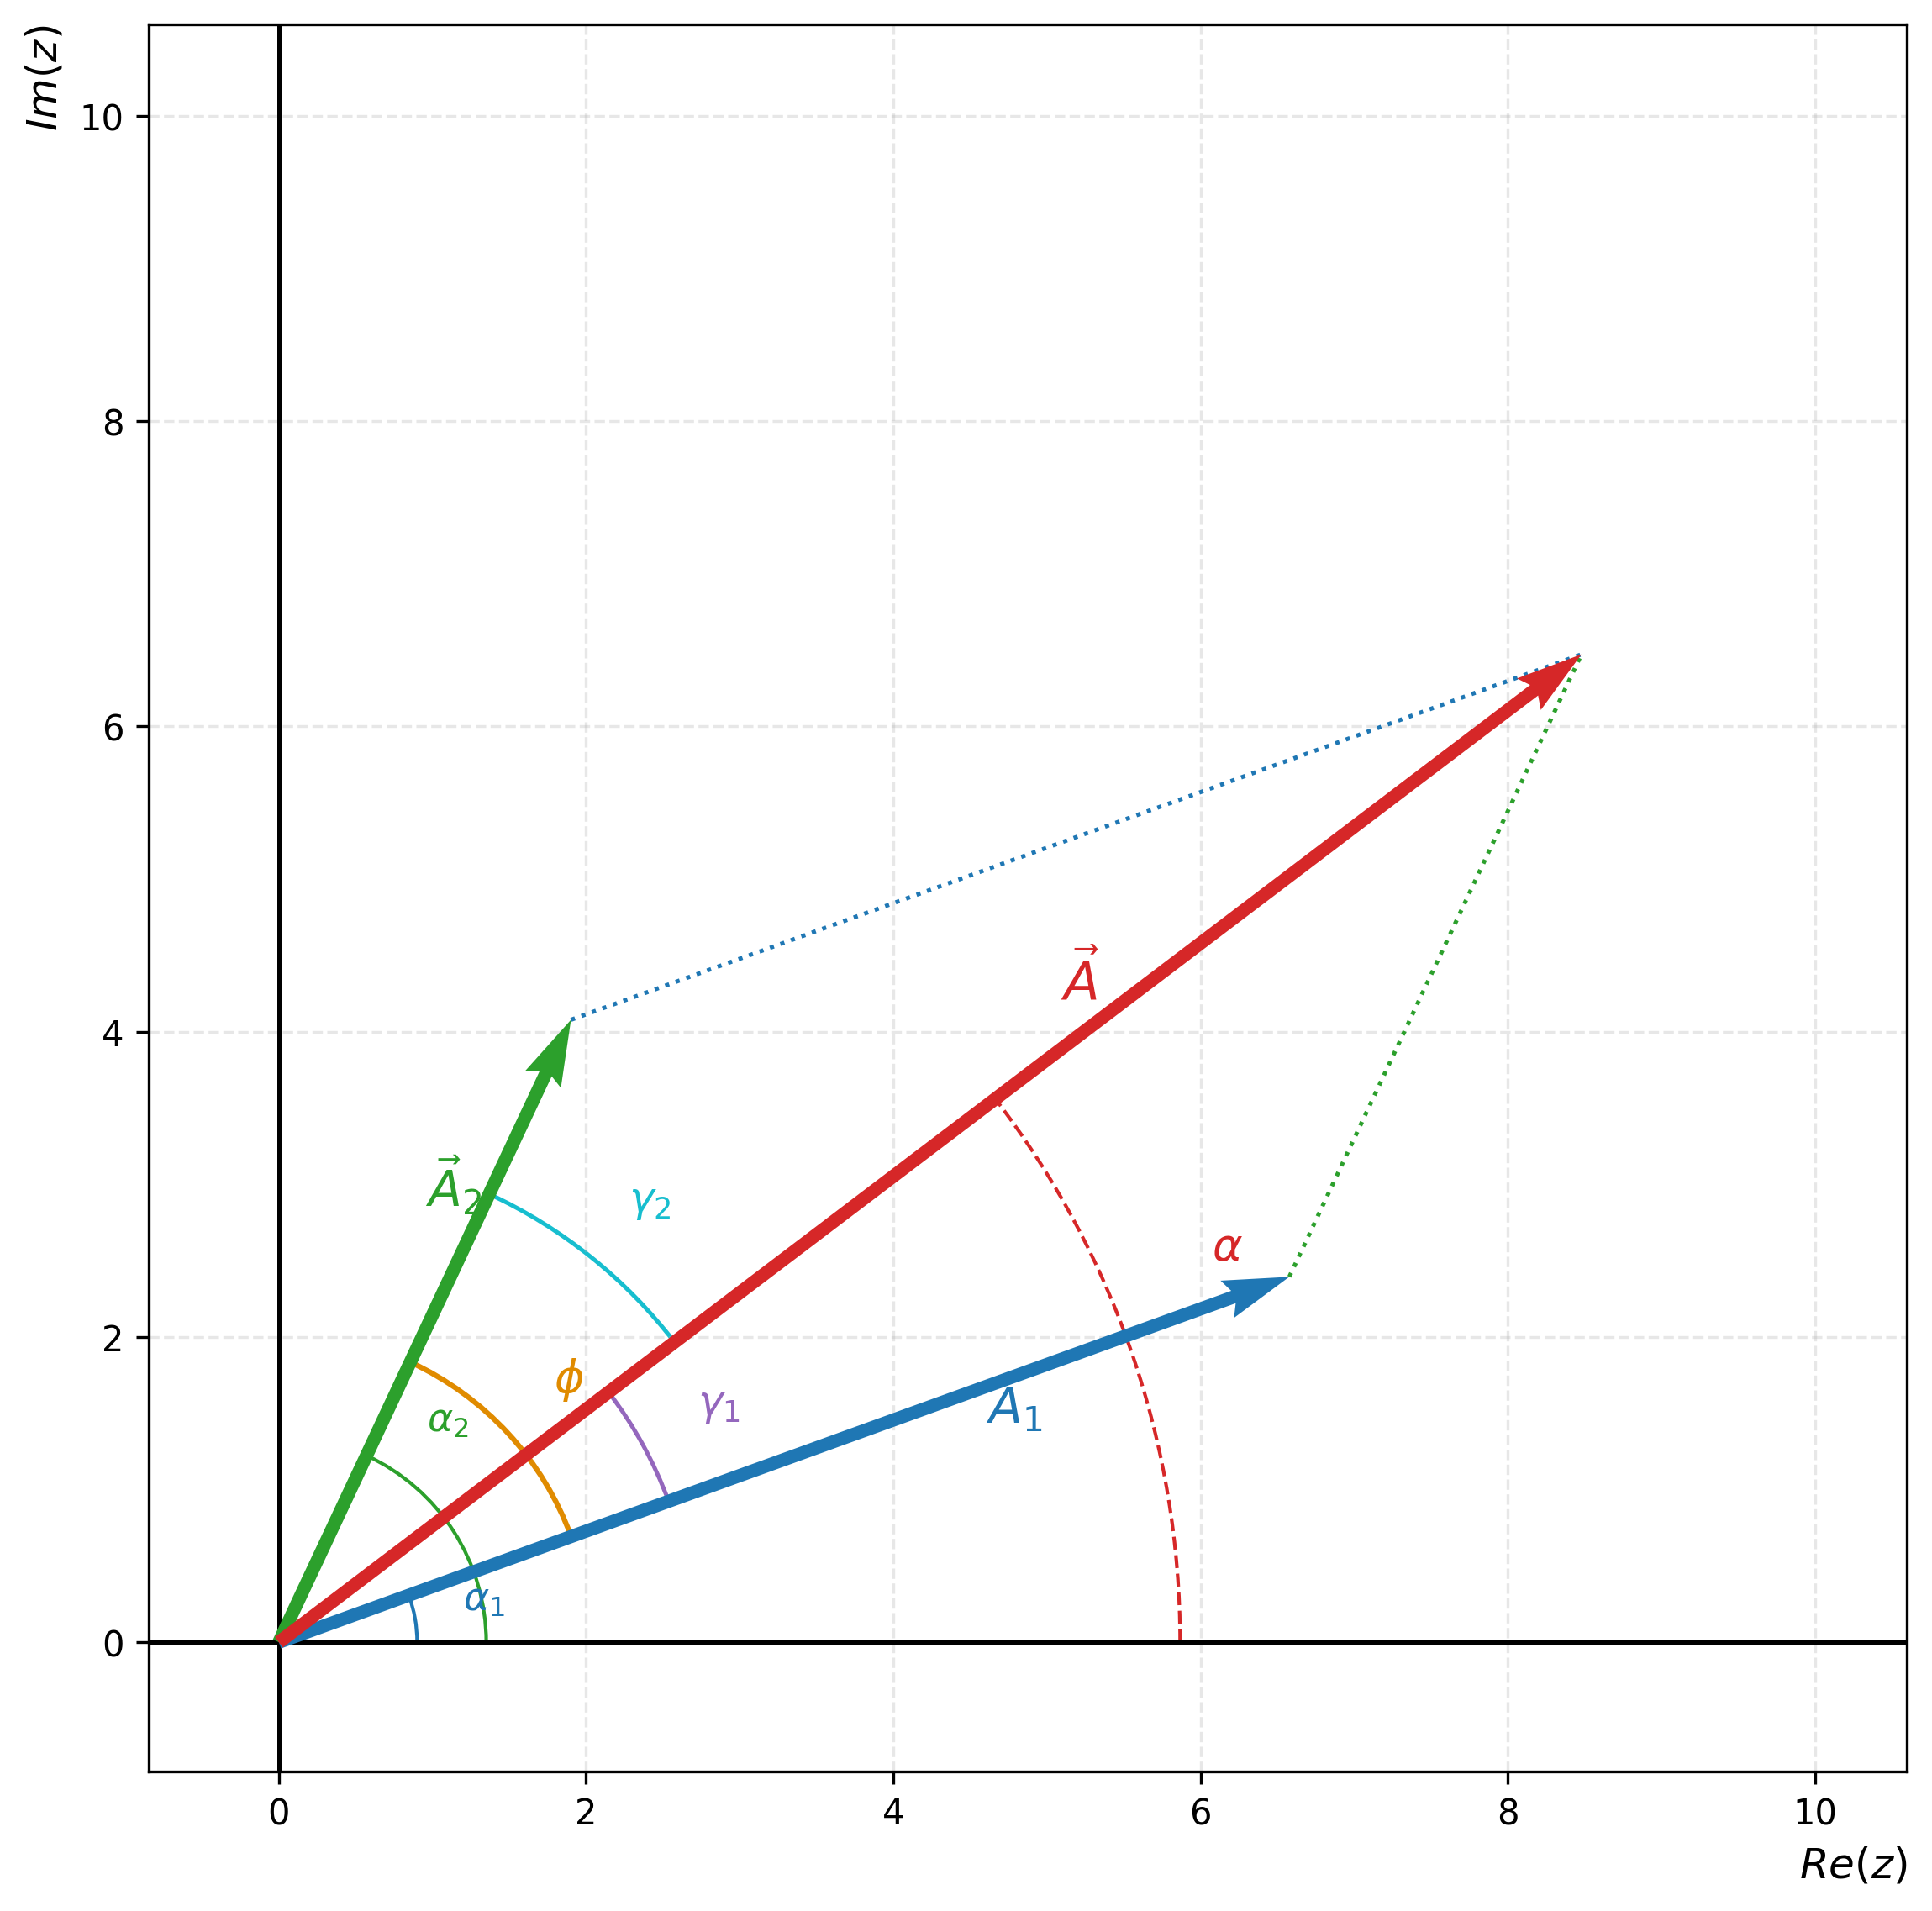
\includegraphics[width=0.6\linewidth]{img/sommaOnde.png}
    \caption{Somma tra le rappresentazioni complesse di onde monocromatiche}
    \label{fig:sommaOnde}
\end{figure}

Studiando quindi, la somma tra $z_1$ e $z_2$ equivale $z$, presente in figura \ref{fig:sommaOnde}, vale che:
\begin{equation}
    A = \sqrt{A_1^2 + A_2^2 + 2A_1A_2\cos(\varphi)}
\end{equation}
mentre vale che:
\begin{equation}
    \begin{cases}
        \varphi = \gamma_1 + \gamma_2 \\
        \alpha = \alpha_1 + \gamma_1 = \alpha_2 - \gamma_2 \\
        A_1 \sin(\gamma_1) = A_2 \sin(\gamma_2)
    \end{cases}
\end{equation}
da cui segue che:
\begin{align}
    f = \Re{z} = A\cos(\alpha) & = \sqrt{A_1^2 + A_2^2 + 2A_1A_2\cos(\varphi)} \cos(\alpha_1 + \gamma_1) \\
    & = \sqrt{A_1^2 + A_2^2 + 2A_1A_2\cos(\varphi)} \cos(kx - \omega t + \gamma_1)
\end{align}

Segue quindi che:
\begin{itemize}
    \item l'ampiezza massima (interferenza costruttiva) equivale a:
    \begin{equation}
        A = A_1 + A_2
    \end{equation}
    ed avviene se e solo se:
    \begin{equation}
        \varphi = 2n\pi, n \in \mathbb{Z}
    \end{equation}
    \item l'ampiezza minima (interferenza distruttiva) equivale a:
    \begin{equation}
        A = |A_1 - A_2|
    \end{equation}
    ed avviene se e solo se:
    \begin{equation}
        \varphi = (2n + 1)\pi, n \in \mathbb{Z}
    \end{equation}
\end{itemize}

Nel caso particolare, ove $A_1 = A_2$, allora:
\begin{align}
    A & = \sqrt{2A_1^2 + 2A_1^2 \cos(\varphi)} \\
      & = 2A_1 \sqrt{\frac{1 + \cos(\varphi)}{2}} \\
      & = 2A_1\cos(\frac{\varphi}{2})
\end{align}
e:
\begin{equation}
    \gamma_1 = \gamma_2 = \frac{\varphi}{2}
\end{equation}
allora, segue che:
\begin{equation}
    f = 2A_1\cos(\frac{\varphi}{2})\cos(kx - \omega t + \frac{\varphi}{2})
\end{equation}
in questo caso, l'ampiezza massima è $2A_1$, mentre l'ampiezza minima è $0$.

\newpage

\section{Sovrapposizione (Battimenti)}
Definendo due onde, come segue:
\begin{align}
    f_1 & = A\cos(k_1 x - \omega_1 t) \\
    f_2 & = A\cos(k_2 x - \omega_2 t)
\end{align}
nel caso in cui le frequenze delle due onde sono vicine, quindi:
\begin{equation}
    |\omega_1 - \omega_2| << \omega_1 + \omega_2 \iff |k_1 - k_2| << k_1 + k_2 
\end{equation}
definendo quindi:
\begin{align}
    \alpha_1 = k_1 x - \omega_1 t \\
    \alpha_2 = k_2 x - \omega_2 t
\end{align}
allora:
\begin{equation}
    \varphi = \alpha_2 - \alpha_1 \not = costante
\end{equation}
Segue quindi che, le relazioni precedenti sono valide istante per istante, quindi:
\begin{equation}
    f = 2A\cos(\frac{\varphi}{2})\cos(k_1x - \omega_1t + \frac{\varphi}{2})
\end{equation}
con:
\begin{equation}
    \alpha_1 + \frac{\varphi}{2} = \alpha_1 - \frac{\alpha_2 - \alpha_1}{2} = \frac{\alpha_1 + \alpha_2}{2}
\end{equation}
segue che:
\begin{equation}
    f = 2A\cos(\frac{k_2 - k_1}{2}x - \frac{\omega_2 - \omega_1}{2}t)\cos(\frac{k_2 + k_1}{2}x - \frac{\omega_2 + \omega_1}{2}t)
\end{equation}
ridefinendo alcune variabili, come segue, si ottiene:
\begin{align}
    k_2 - k_1 & \equiv \Delta k \\
    \omega_2 - \omega_1 & \equiv \Delta \omega \\
    \frac{k_1 + k_2}{2} & \equiv k_0 \\
    \frac{\omega_1 + \omega_2}{2} & \equiv \omega_0
\end{align}

\begin{equation}
    f = 2A\cos(\frac{\Delta k}{2}x - \frac{\Delta \omega}{2}t)\cos(k_0x - \omega_0t)
\end{equation}

Studiando le propagazioni spaziali (fissando il tempo) e quelle temporali (fissando lo spazio), si possono visualizzare i battimenti.
\begin{itemize}
    \item Nel caso temporale, l'onda è descritta da:
        \begin{equation}
            f(0, t) = 2A\cos(\frac{\Delta \omega}{2}t)\cos(\omega_0 t)
        \end{equation}

        \begin{figure}[H]
            \centering
            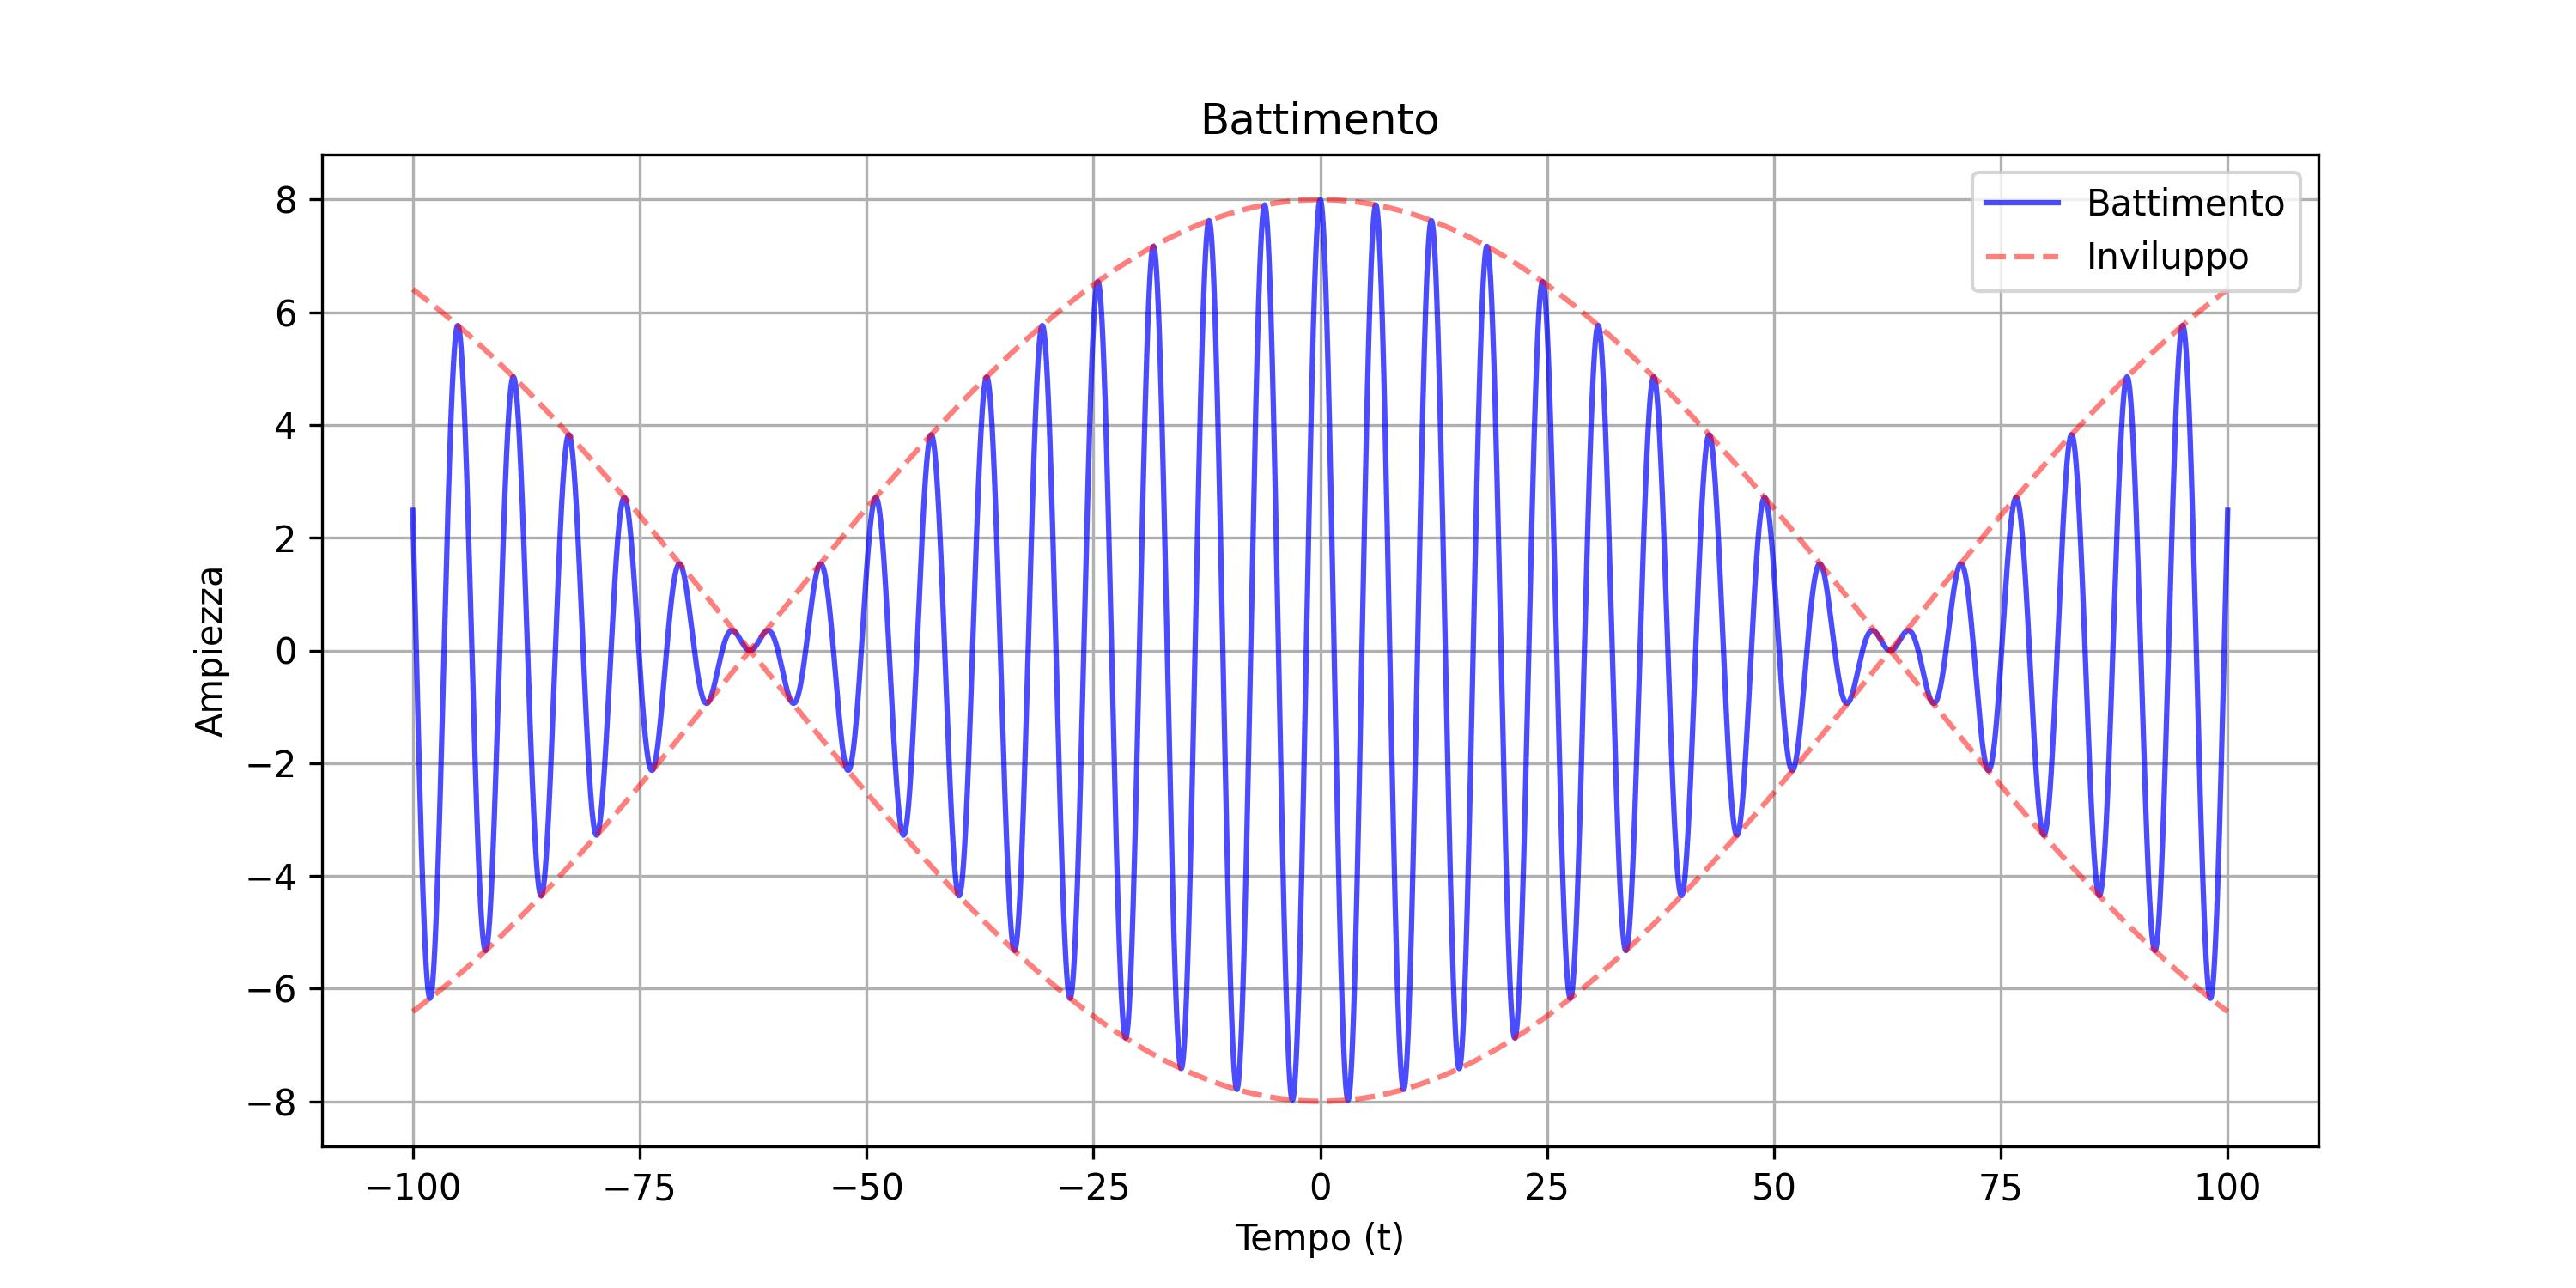
\includegraphics[width=1\linewidth]{img/battimentoTemporale.jpg}
            \caption{Battimenti temporali (con spazio fissato)}
            \label{fig:battimentoTemporale}
        \end{figure}
    \item Nel caso temporale invece, l'onda è descritta da:
        \begin{equation}
            f(x, 0) = 2A\cos(\frac{\Delta k}{2}x)\cos(k_0 x)
        \end{equation}

        \begin{figure}[H]
            \centering
            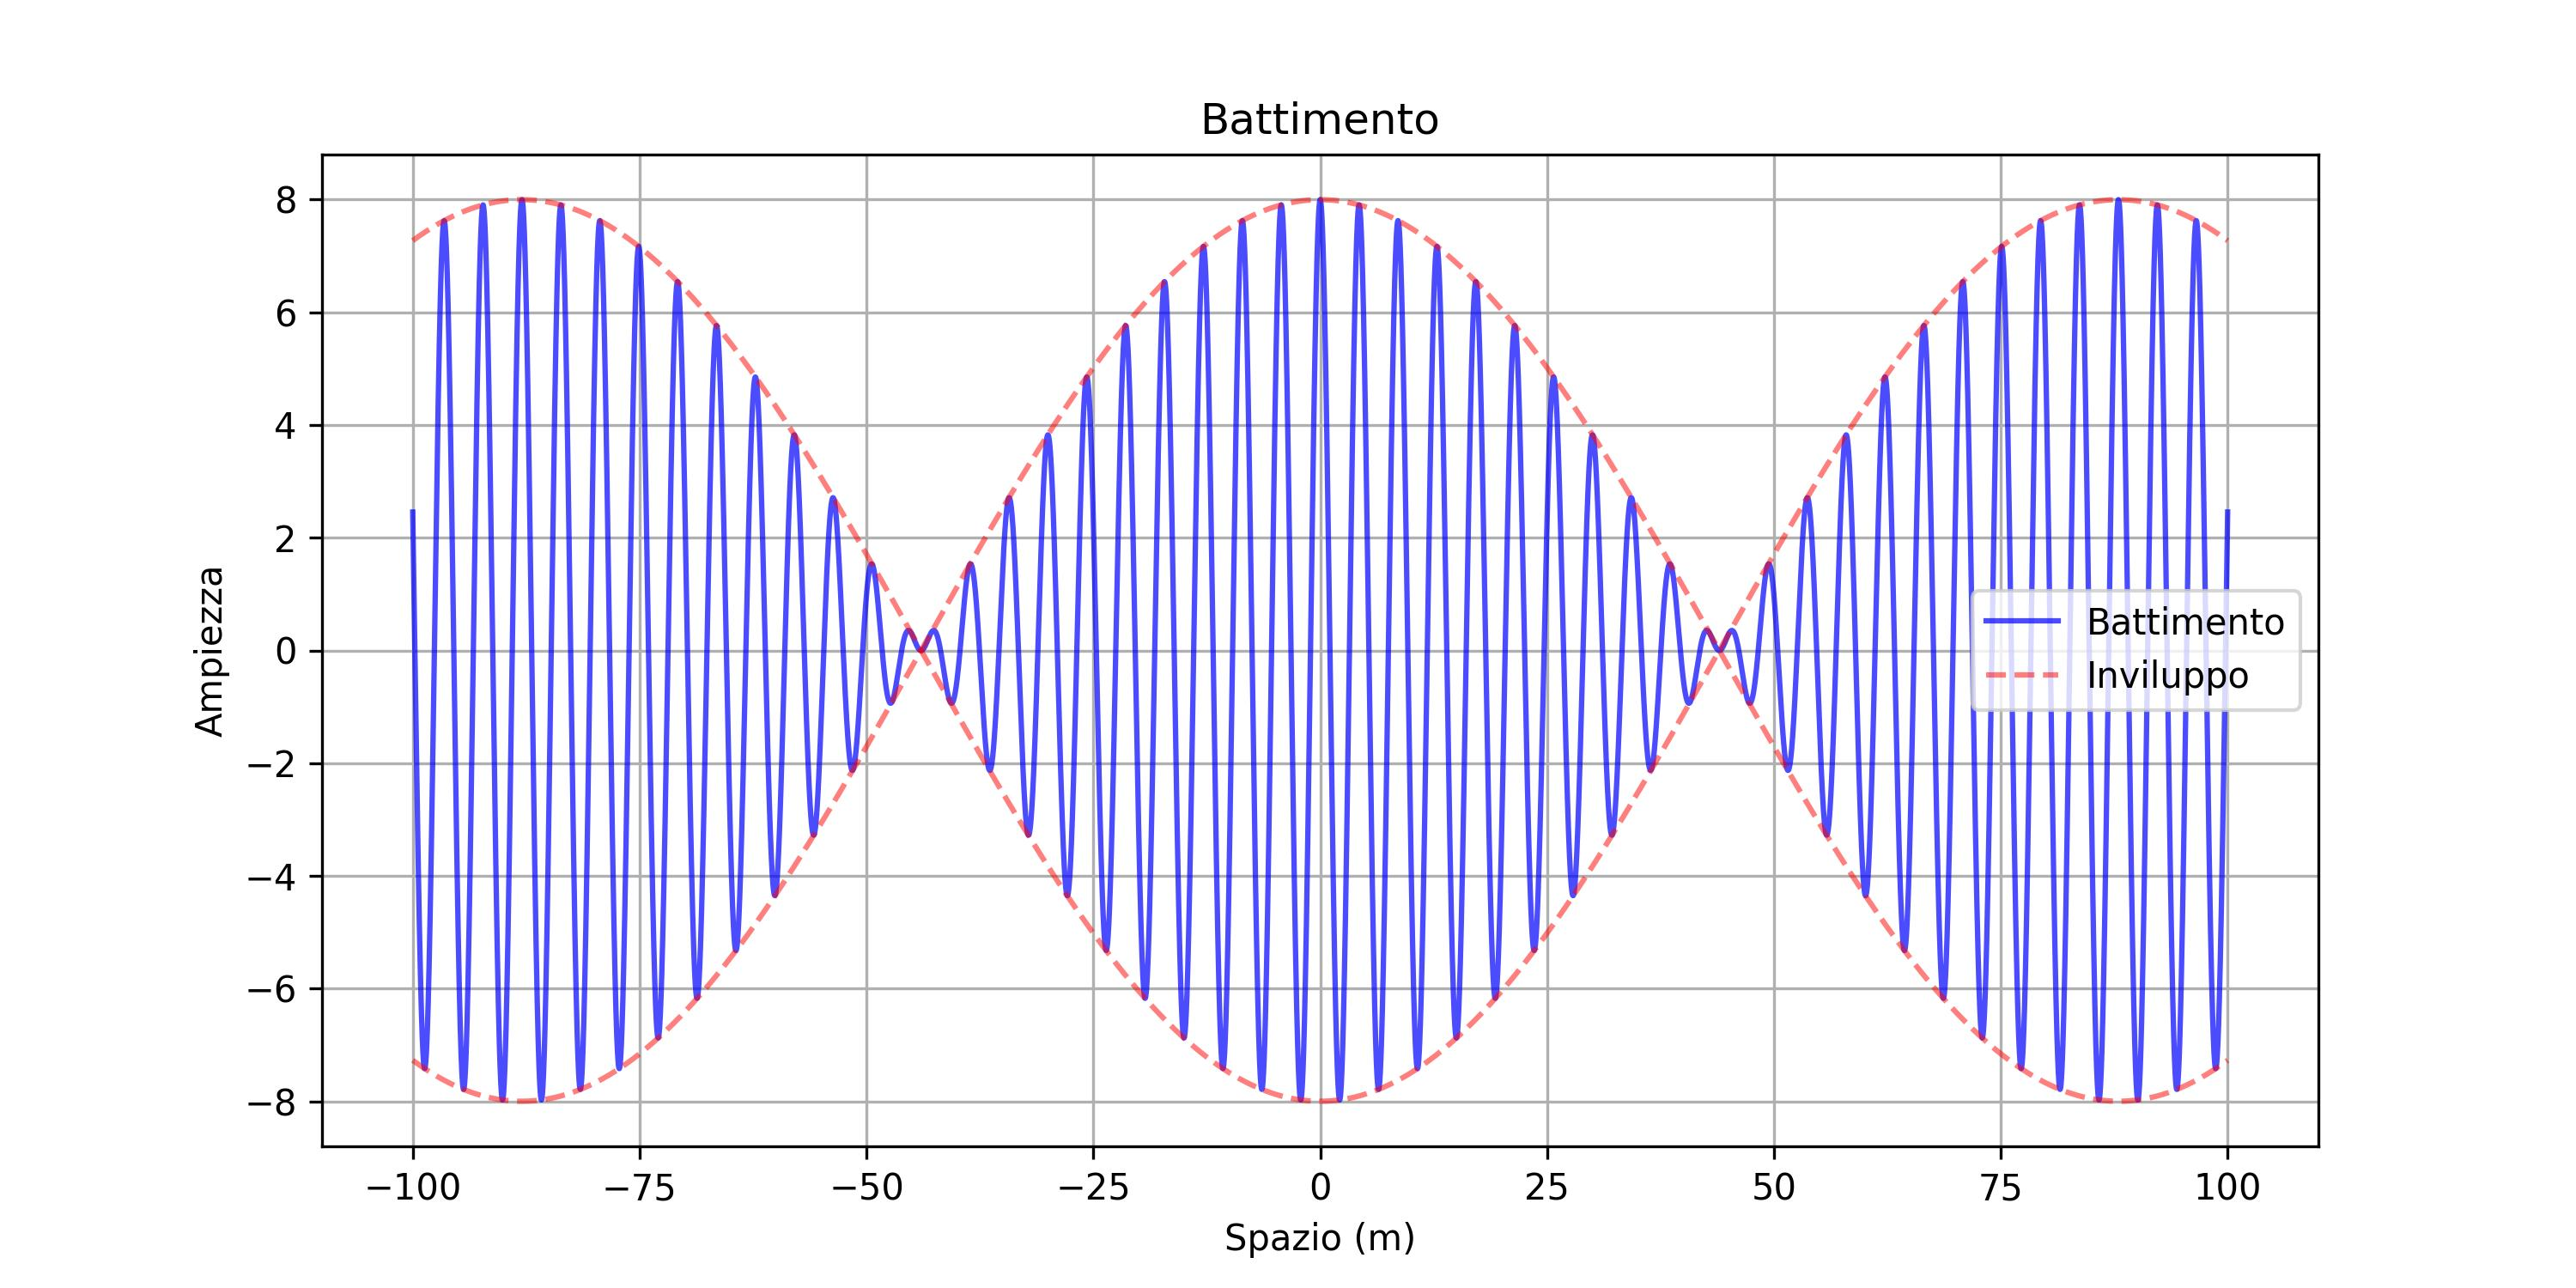
\includegraphics[width=1\linewidth]{img/battimentoSpaziale.jpg}
            \caption{Battimenti spaziali (con tempo fissato)}
            \label{fig:battimentoSpaziale}
        \end{figure}

        Si può inoltre definire una ulteriore quantità, ovvero la velocità di gruppo:
        \begin{equation}
            v_g = \frac{\Delta\omega}{\Delta k } = v
        \end{equation}

\end{itemize}


\newpage

\section{Fenomeni di dispersione}
I fenomeri di dispersione sono fenomeni per cui onde monocromatiche con pulsazioni diverse hanno velocità di fase diverse, infatti la velocità di fase dipende dalla pulsazione. Sono quindi onde che vengono descritte da equazioni di D'Alambert con $v$ diversa.

In generale ogni mezzo è dispersivo, tranne il vuoto.

% DA COMPRENDERE

\section{Onde trasversali nella corda (approssimazione per piccola perturbazioni)}
Se si considera una corda che all'equilibrio è tesa in configurazione perfettamente orizzontale, definendo $\xi(x, t)$ come la funzione che descrivere lo spostamento lungo y di un tratto dx centrato in x all'istante t.

Allora trascurando la forza peso e definendo la densità di massa lineare $\sigma = \frac{dm}{dx}$, allora dalla seconda legge di Newton segue che:
\begin{equation}
    \vec{T}(x + dx) + \vec{T}(x) = \sigma dx \vec{a}
\end{equation} 
ma poiché il moto è verticale (accelerazione lungo x nulla), allora proiettando lungo x:
\begin{equation}
    T(x + dx)\cos(\theta + d\theta) - T(x)\cos(\theta) = a_x = 0
\end{equation}
nell'approssimazione per piccole perturbazioni, è possibile sviluppare il coseno con tramite gli sviluppi di Taylor-McLauren al primo ordine, dove segue che:
\begin{equation}
    \cos(\theta) = \cos(\theta + d\theta) = 1
\end{equation}

allora:
\begin{equation}
    T(x + dx) = T(x) = T
\end{equation}

Proiettando invece lungo l'asse y:
\begin{equation}
    T\sin(\theta + d\theta) - T\sin(\theta) = \sigma dx a_y
\end{equation}
applicando nuovamente gli sviluppi di Taylor, segue che \textit{PER $\theta$ PICCOLI}:
\begin{equation}
    \sin(\theta + d\theta) - \sin(\theta) = (\theta + d\theta) - \theta \simeq \tan(\theta + d\theta) - \tan(\theta)
\end{equation}
da cui segue che:
\begin{equation}
    T(\tan(\theta + d\theta) - \tan(\theta)) = \sigma dx a_y
\end{equation}

Per le proprietà delle derivate, vale che:
\begin{align}
    a_y & = \pdv[2]{\xi}{t} \\
    \tan(\theta) = \pdv{\xi}{x}
\end{align}
allora:
\begin{equation}
    \tan(\theta + d\theta) - \tan(\theta) = \eval{\pdv{\xi}{x}}_{x + dx}^{} - \eval{\pdv{\xi}{x}}_{x}^{}
\end{equation}
da cui segue che:
\begin{equation}
    \frac{T(\eval{\pdv{\xi}{x}}_{x + dx}^{} - \eval{\pdv{\xi}{x}}_{x}^{})}{dx} = \sigma \pdv[2]{\xi}{t}
\end{equation}
per la definizione della derivata tramite il processo di limite del rapporto incrementale, allora:
\begin{equation}
    T\pdv[2]{\xi}{x} = \sigma \pdv[2]{\xi}{t}
\end{equation}
definendo:
\begin{equation}
    v = \sqrt{\frac{T}{\sigma}}
\end{equation}
allora si ottiene l'equazione d'onda di D'Alambert, infatti:
\begin{equation}
    \pdv[2]{\xi}{x} = \frac{1}{v^2} \pdv[2]{\xi}{t}
\end{equation}

\section{Energia dell'onda}
Considerando un tratto infinitesimo di corda, allora il lavoro infinitesimo della tensione applicata da sinistra è:
\begin{align}
    \delta L & = \vec{T} \cdot d\vec{r} \\
             & = T_y \cdot d\xi \\
             & = T_y \pdv{\xi}{t} dt
\end{align}
Ciò corrisponde quindi alla potenza moltiplicata per un tempo infinitesimo, infatti:
\begin{equation}
    P(x, t) = T_y \pdv{\xi}{t}
\end{equation}
allora:
\begin{equation}
    \delta L = P(x, t)dt
\end{equation}
considerando che:
\begin{equation}
    T_y = -T\sin(\theta) = -T\tan(\theta) = -T \pdv{\xi}{t}
\end{equation}
allora:
\begin{equation}
    P(x, t) = - T \pdv{\xi}{x}\pdv{\xi}{t}
\end{equation}

Sapendo che:
\begin{align}
    v^2 & = \frac{T}{\sigma} \\
    \pdv{\xi}{x} & = -\frac{1}{v} \pdv{\xi}{t}
\end{align}
allora:
\begin{align}
    P(x, t) & = \frac{T}{v}\left(\pdv{\xi}{t}\right)^2 \\
            & = v\sigma\left(\pdv{\xi}{t}\right)^2 \\
            & = Tv\left(\pdv{\xi}{x}\right)^2
\end{align}
da cui:
\begin{equation}
    P(x, t) = v\left[\frac{1}{2}\sigma\left(\pdv{\xi}{t}\right)^2 + \frac{1}{2}T\left(\pdv{\xi}{x}\right)^2\right]
\end{equation}
\begin{align}
    \Longrightarrow \delta L & = vdt\left[\frac{1}{2}\sigma\left(\pdv{\xi}{t}\right)^2 + \frac{1}{2}T\left(\pdv{\xi}{x}\right)^2\right] \\
    & = dx\left[\frac{1}{2}\sigma\left(\pdv{\xi}{t}\right)^2 + \frac{1}{2}T\left(\pdv{\xi}{x}\right)^2\right] \\
    & = \frac{1}{2}\sigma\left(\pdv{\xi}{t}\right)^2dx + \frac{1}{2}T\left(\pdv{\xi}{x}\right)^2dx
\end{align}
nella quale:
\begin{itemize}
    \item Il primo termine $\displaystyle \frac{1}{2}\sigma\left(\pdv{\xi}{t}\right)^2dx$ rappresenta l'energia cinetica del tratto $dx$.
    \item Il secondo $\displaystyle \frac{1}{2}T\left(\pdv{\xi}{x}\right)^2dx$ equivale all'energia potenziale del tratto di corda.
\end{itemize}

È quindi possibile definire una nuova quantità, ovvero la densità di energia:
\begin{equation}
    U(x, t) = \frac{1}{2}\sigma\left(\pdv{\xi}{t}\right)^2 + \frac{1}{2}T\left(\pdv{\xi}{x}\right)^2
    \label{eq:densitàDiEnergia}
\end{equation}
da cui:
\begin{equation}
    P(x, t) = vU(x, t)
    \label{eq:potenza}
\end{equation}

% AGGIUNGERE CONSIDERAZIONI SUL TRATTO DESTRO

\subsection{Energia e potenza nelle onde monocromatiche}
Nel caso di un'onda piana monocromatica, come già visto descritta da:
\begin{equation}
    \xi(x, t) = A\cos(kx - \omega t)
\end{equation} 
la densità di energia e la potenza si calcolano immediatamente dalle formule \ref{eq:densitàDiEnergia} e \ref{eq:potenza}, da cui segue che:
\begin{align}
    U(x, t) & = \sigma\left(\pdv{\xi}{t}\right)^2 = \sigma \omega^2 A^2 \sin^2(kx - \omega t) \\
    P(x, t) & = vU(x, t) = v\sigma \omega^2 A^2 \sin^2(kx - \omega t)
\end{align}

\subsubsection{Onde monodimensionali (caso della corda)}
Si verifica facilmente che sia $U(x, t)$ sia $P(x, t)$ soddisfano l'equazione di D'Alambert e quindi che si propagano con velocità $v$ lungo la corda, la quale è confrontabile con una onda piana in buona approssimazione.

Per mantenere un'onda sinusoidale, biosgna fornire energia con continuità facendo oscillare un estremo della corda (supponendo che essa sia molto lunga).

È quindi possibile calcolare l'energia che deve essere trasferita alla corda in un periodo per mantenere l'oscillazione, trascurando l'attrito con l'aria, per farlo è possibile integrare su un periodo $T$ la potenza calcola nell'estremo della corda ($x = 0$), allora:
\begin{align}
    E_T & = \int_{t_0}^{t_0 + T} P(0, t) dt \\
        & = \int_{t_0}^{t_0 + T} v\sigma\omega^2A^2\sin^2(\omega t) dt \\
        & = \frac{\pi}{\omega}\sigma v \omega^2A^2; \quad \omega = kv \\
        & = \frac{\pi}{k}\sigma\omega^2A^2 \\
        & = \frac{1}{2}\frac{2\pi}{k}\sigma\omega^2A^2; \quad \lambda = \frac{2\pi}{k} \\
        & = \frac{1}{2}\lambda\sigma\omega^2A^2
\end{align}
Calcolando l'energia totale di un tratto di corda oscillante di lunghezza $\lambda$ ad un instante generico, si otttiene:
\begin{align}
    E_\lambda & = \int_{x}^{x + \lambda} U(x, t)dx \\
              & = \int_{x}^{x + \lambda} \sigma \omega^2 A^2 \sin^2(kx - \omega t)dx \\
              & = \frac{1}{2}\sigma A^2 \omega^2 \lambda \\
              & = E_T
\end{align}
Pertanto si conclude che:
\begin{itemize}
    \item la sorgente della perturbazione immette continuamente energia nella corda, aumentando l'energia totale della stessa. L'energia immessa è pasi a $\displaystyle \frac{1}{2}\sigma A^2 \omega^2 \lambda$ per periodo $T$
    \item in un periodo $T$ la perturbazione avanza di un tratto $\lambda = vt$
    \item tale energia corrisponde anche all'energia totale di un tratto di corda oscillante (ovvero già perturbato) di lunghezza $\lambda$
\end{itemize}
È interessante notare che:
\begin{itemize}
    \item Nel caso di onde sinusoidali, solitamente vengono considerate quantità mediate su un periodio, da cui segue che la potenza media è:
    \begin{equation}
        \bar{P} = \frac{E_T}{T} = \frac{1}{2}\sigma\lambda A^2\omega^2
    \end{equation}
    \item L'energia $E_\lambda = \frac{1}{2}\sigma\lambda A^2\omega^2$ corrisponde all'energia totale di un oscillatore armonica di massa $m = \sigma\lambda$, però in questo caso a differenza di un oscillatore armonico per ogni tratto infinitesimo di corda l'energia cinetica e l'energia potenziale sono sempre uguali tra loro.
\end{itemize}

\newpage

\section{Onde stazionarie}
Per comprendere le onde stazionarie è possibile studiare il caso di un onda trasversale su una corda, supponendo di generare un onda muovendo l'estremo sinistro, allora il comportamento dell'onda una volta raggiunto l'estremo destro è diverso a seconda che esso sia fisso o mobile.

L'onda viene riflessa in entrambi i casi ma in maniera diversa, infatti:
\begin{itemize}
    \item se l'estremo è fisso, lo spostamento trasversale in quel punto è nullo ad ogni istante, ciò è possibile solo se è presente un'onda riflessa che si sovrappone all'onda incidente e la "cancella" in modo tale che la loro somma sia nulla. Pertanto l'onda riflessa deve essere invertita rispetto a quella incidente.
    \item se l'estremo è mobile, allora l'onda riflessa \textit{non} è invertita.
\end{itemize}

Se non vi è trasferimento di energia ai vincoli, o nel caso in cui non vi è attrito per l'estremo mobile, l'onda viene riflessa integralmente.

Se si generano altre onde incidenti dopo la prima, esse si sovrappongono a quelle riflesse, ciò corrisponde a una soluzione dell'equazione d'onda del tipo:
\begin{equation}
    \xi(x, t) = f(x - vt) + g(x + vt)
\end{equation}

Studiando quindi la sovrapposizione tra due onde (incidente e riflessa) monocromatiche, è possibile supporre che le due onde abbiamo la stessa ampiezza e pulsazione, ma velocitò opposte, quindi siamo in presenza di un onda progressiva e una regressiva.

Considerando entrambi i casi di onde riflessa invertita e non, allora abbiamo:
\begin{equation}
    f = A\cos(kx - \omega t); \quad \quad g = \pm A\cos(kx + \omega t)
\end{equation}
sommando le due onde, si ottiene la relazione trigonometrica:
\begin{equation}
    \cos(\alpha \pm \beta) = \cos(\alpha)\cos(\beta) \mp \sin(\alpha)\sin(\beta)
\end{equation}
infatti:
\begin{equation}
    \xi_\pm = A\cos(kx - \omega t) \pm A\cos(kx + \omega t) = \begin{cases}
        2A\cos(kx)\cos(\omega t); \quad \text{estremo libero} \\
        2A\sin(kx)\sin(\omega t); \quad \text{estremo fisso} \\
    \end{cases}
    \label{eq:ondaStazionaria}
\end{equation}
Supponendo che l'estremo destro della corda si trovi a $x = 0$, otteniamo il seguente comportamento nei due casi:
\begin{itemize}
    \item Estremo libero:
    \begin{equation}
        \xi_+(0, t) = 2A\cos(\omega t)
    \end{equation}
    \item Estremo fisso:
    \begin{equation}
        \xi_-(0, t) = 0
    \end{equation}
\end{itemize}
Le equazioni \ref{eq:ondaStazionaria} descrivono un onda stazionario, che non si propaga in un verso determinato, infatti la corsa si comporta come un'unica entità vibrante e tutti i punti vibrano in fase, ma con ampiezze diverse.

In particolare vi sono dei punti, detti nodi, in cui $\xi = 0 \; \forall t$ e dei punti, detti ventri, dove la deformazione è massima in ogni istante, rappresentati in figura \ref{fig:ondeStazionarie}.

\begin{figure}[H]
    \centering
    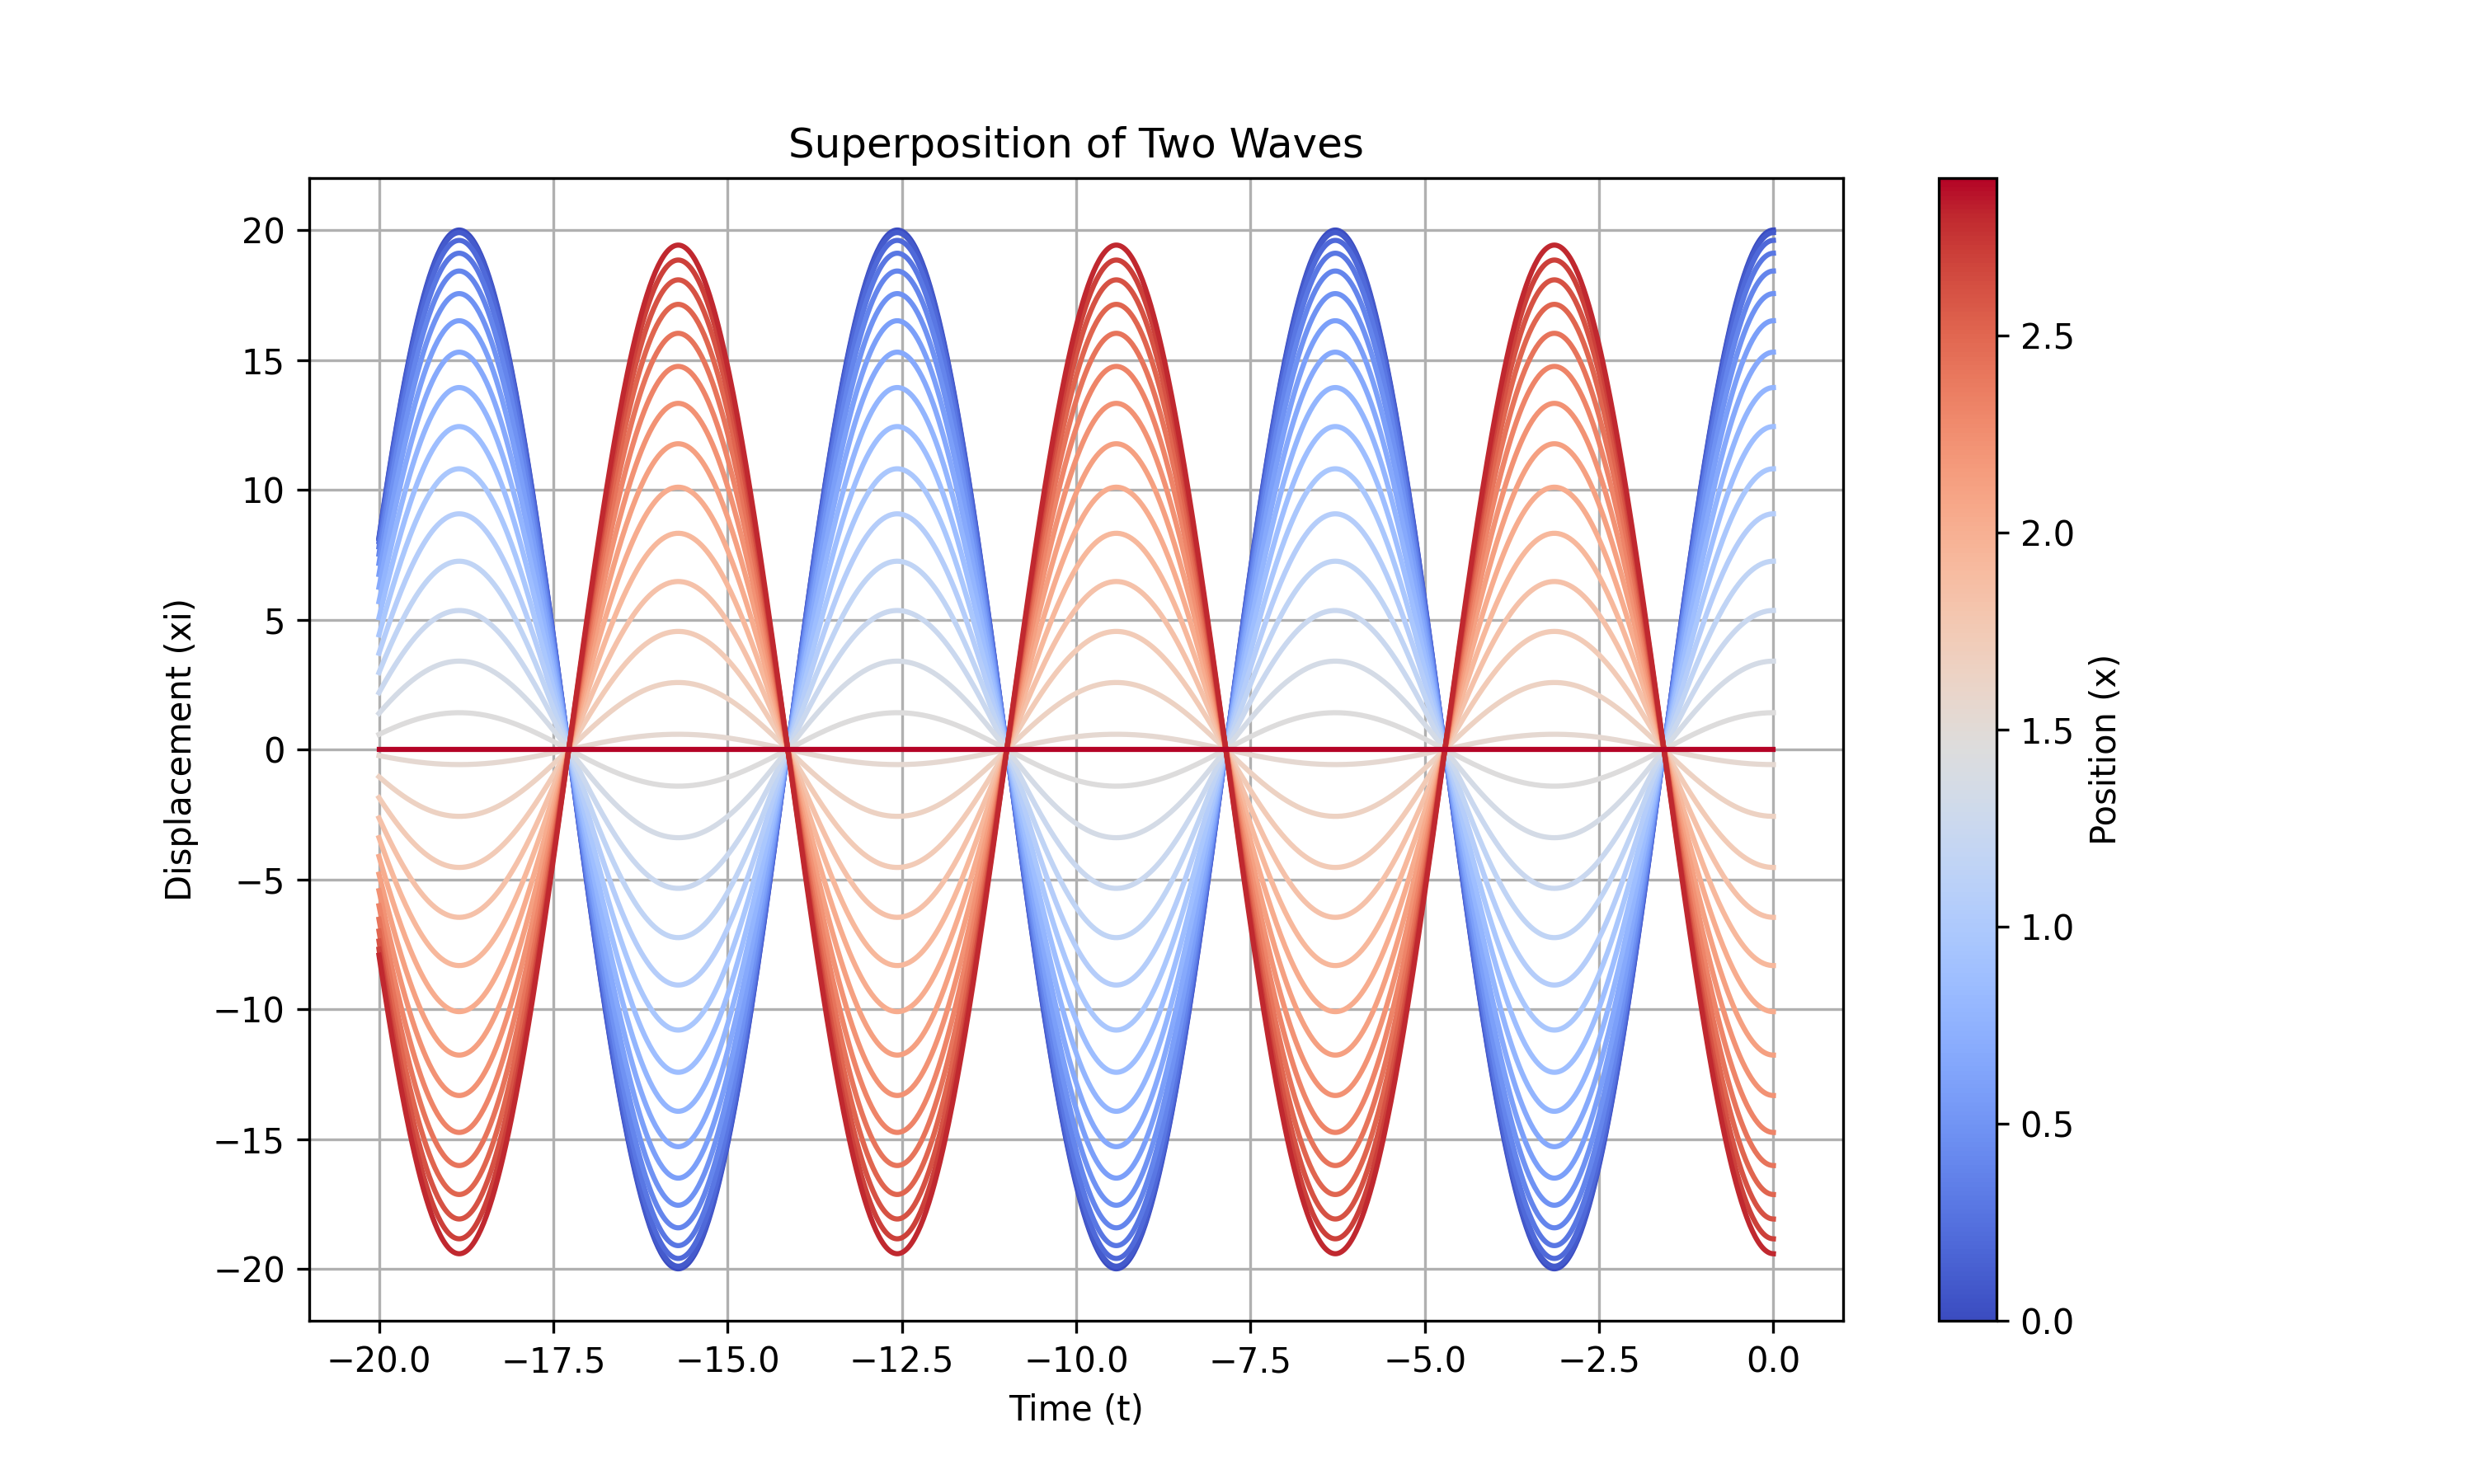
\includegraphics[width=1\linewidth]{img/onde_stazionarie.png}
    \caption{Grafico del displacement in funzione del tempo, al variare della x fissata}
    \label{fig:ondeStazionarie}
\end{figure}

\subsection{Onde stazionarie su una corda di lunghezza $L$ con estremi fissi}
Tali considerazioni valgono per una corda di lunghezza arbitraria, considerando un corda di lunghezza $L$ e supponendo che entrambi gli estremi della corda siano fissi, come negli strumenti a corda.

Le onde stazionarie con estremi fissi, devono avere nodi agli estremi $x = 0$ e $x = L$, segue quindi che:
\begin{equation}
    \xi(0, t) = 0; \quad \xi(L, t) = 0; \; \; \forall t
\end{equation}
la prima condizione è soddisfatta per:
\begin{equation}
    \xi(x, t) = A\sin(kx)\sin(\omega t) 
\end{equation}
la seconda è soddisfatta se:
\begin{equation}
    \sin(kL) = 0 \implies kL = n\pi, n \in \mathbb{N}^+
\end{equation}
dalla quale segue che:
\begin{equation}
    k_n = \frac{n\pi}{L}, n \in \mathbb{N}^+ \implies \lambda_n = \frac{2L}{n}, n \in \mathbb{N}^+
\end{equation}
Ciò significa che la corda deve contenenre un numero interno di mezze lunghezze d'onda:
\begin{equation}
    L = n \frac{\lambda_n}{2}, \; n \in \mathbb{N}^+
\end{equation}
A valori discreti di $\lambda_n$ corrispondono valori discretti di $\omega = vk = \frac{2\pi v}{\lambda}$ e della frequenza $\nu = \frac{\omega}{2\pi}$, infatti:
\begin{equation}
    \omega_n = \frac{\pi vn}{L} = n\omega_1; \quad \quad \nu_n = \frac{vn}{2L}, \quad n \in \mathbb{N}^+
\end{equation}

tali valori sono detti autofrequenze o frequenze naturali della corda. La frequenza $\nu_1$ è detta fondamentale, le altre sono dette armoniche.

Le onde stazionarie corrispondenti alle varie armoniche, dette \textit{modi normali} di vibrazione, hanno la forma:

\begin{equation}
    \xi(x, t) = A_n \sin(k_nx)\sin(\omega_nt); \quad n \in \mathbb{N}^+
\end{equation}

\begin{figure}[h]
    \centering
    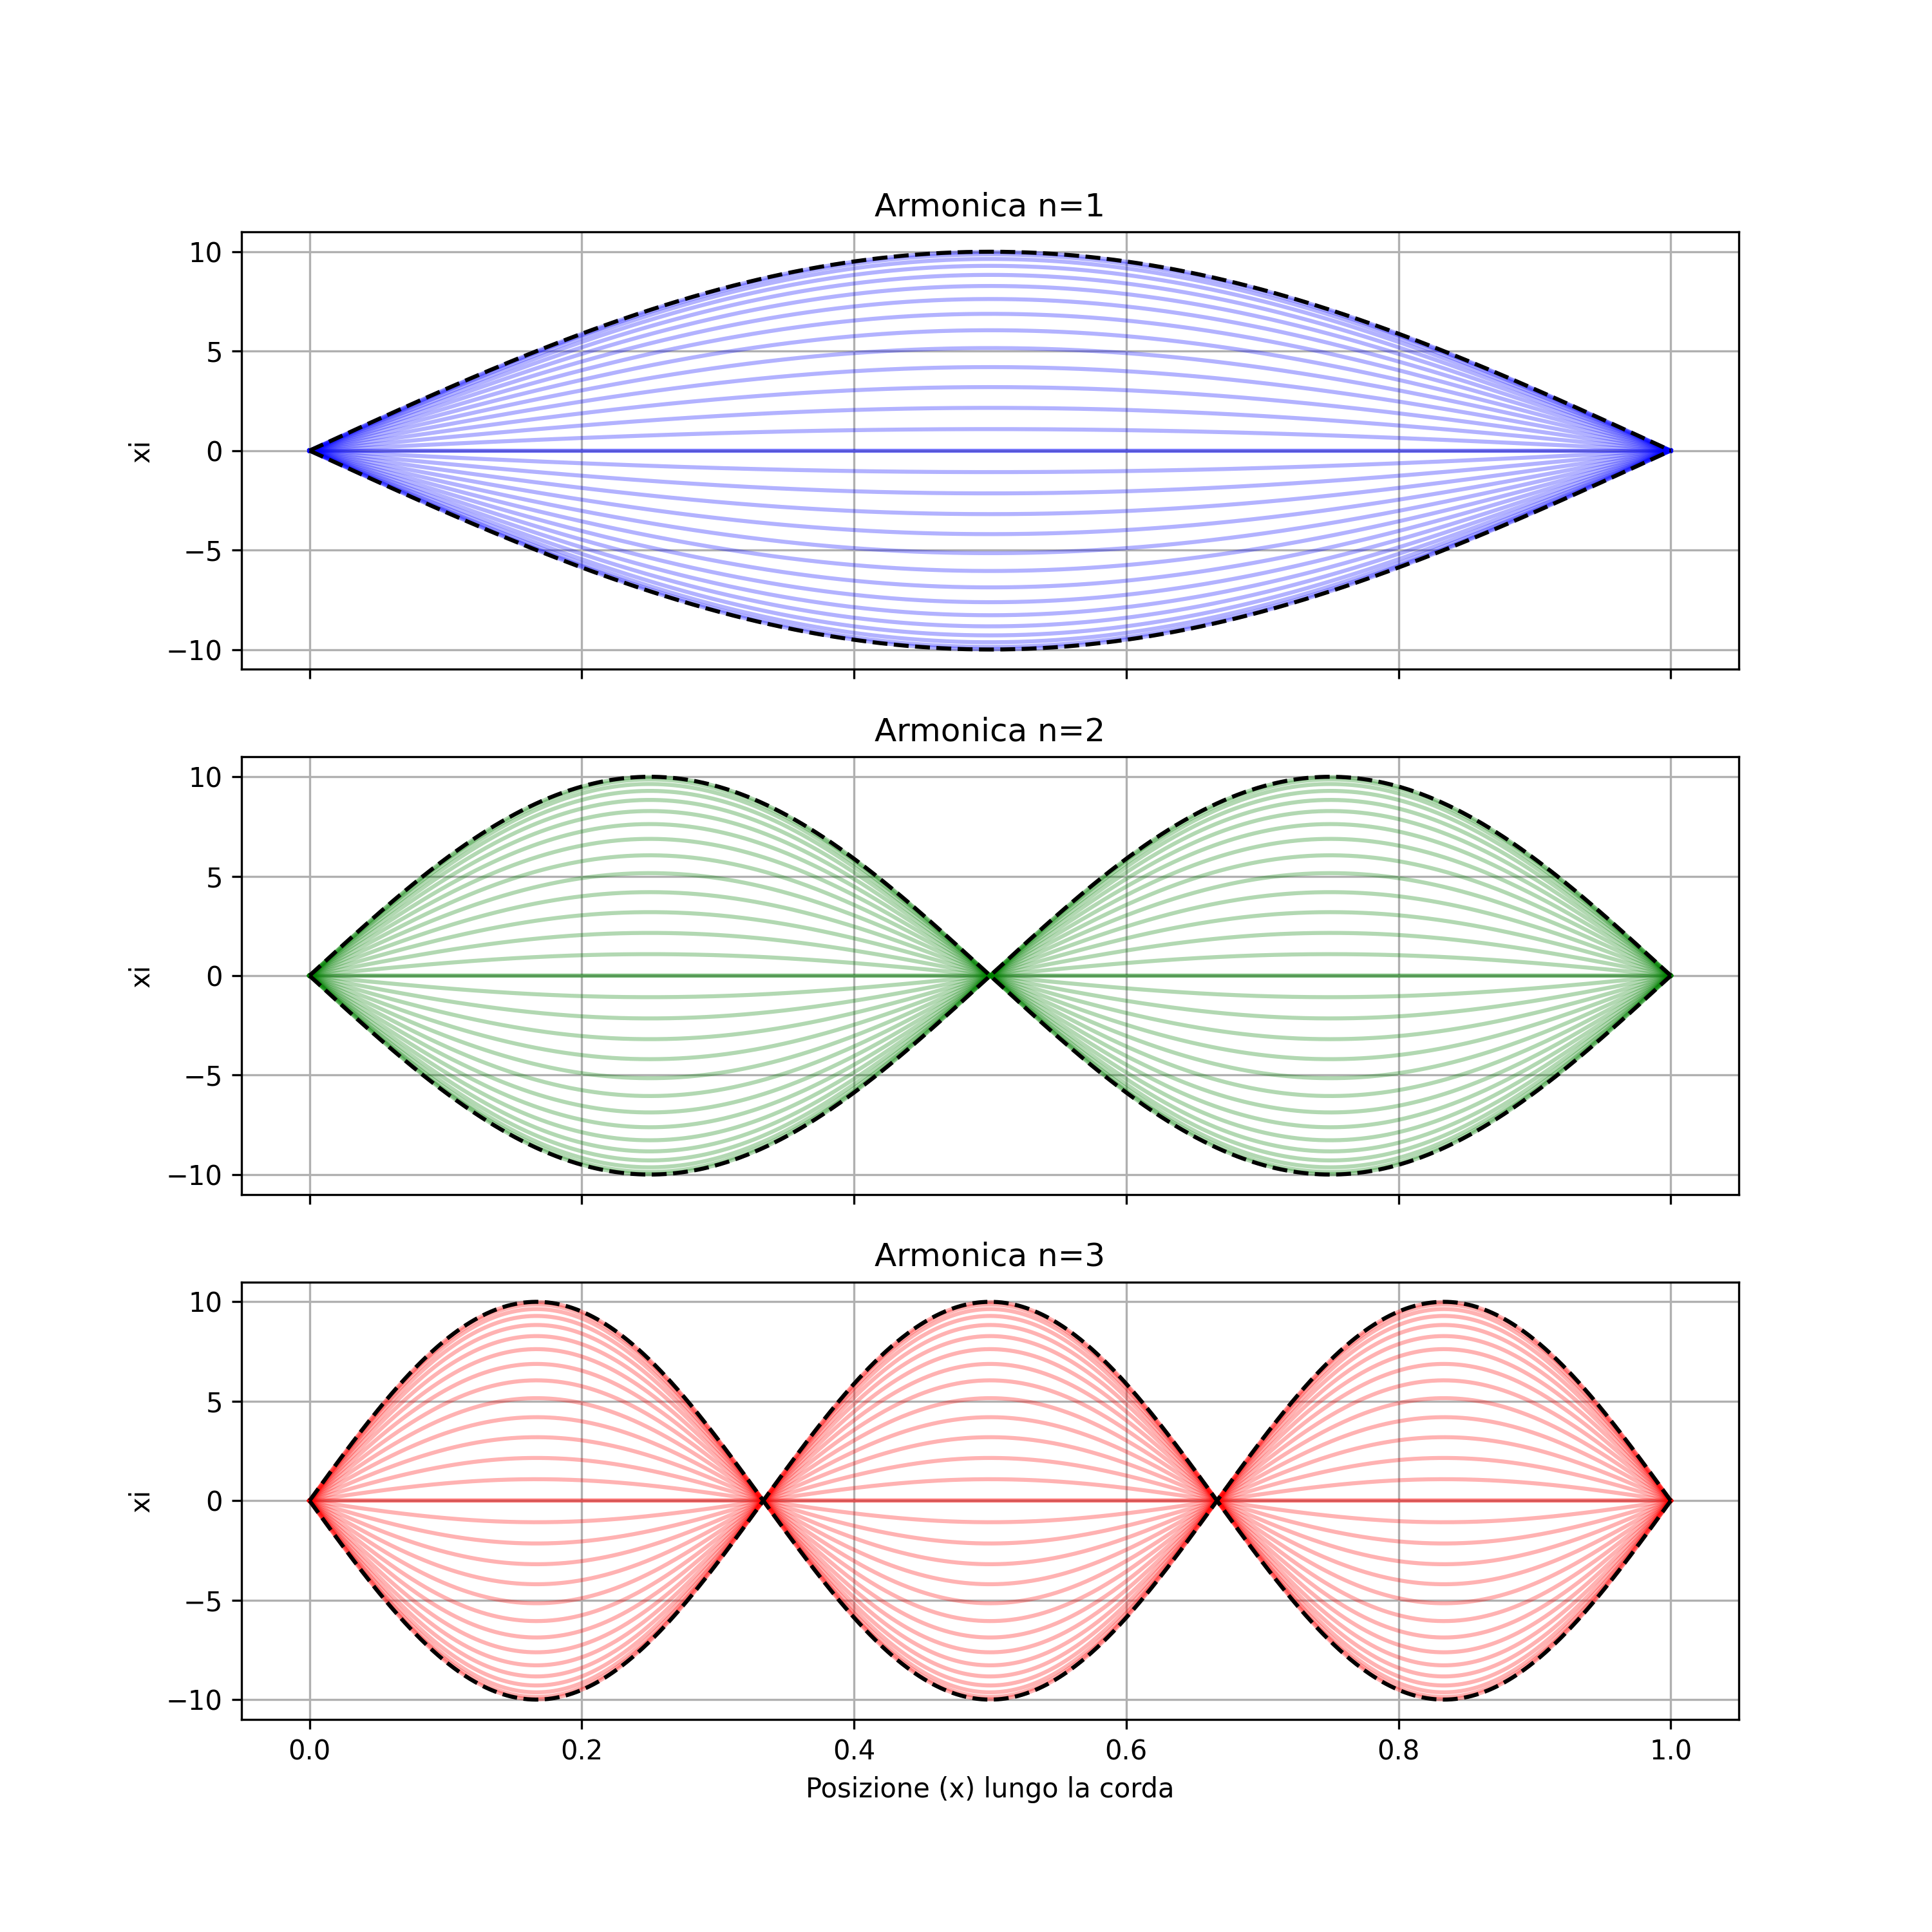
\includegraphics[width=0.7\linewidth]{img/armonicheCorda.png}
    \caption{Le 3 armoniche corrispondenti a $n = 1, 2, 3$<}
    \label{fig:armonicheCorda}
\end{figure}

Nella figura \ref{fig:armonicheCorda} sono presenti 3 onde stazionarie corrispondenti a $n = 1, 2, 3$ con lunghezze d'onda e frequenze rispettivamente pari a:
\begin{align}
    \lambda_1 &= 2L & \lambda_2 &= L & \lambda_3 &= \frac{2}{3}L \\
    \nu_1 &= \frac{v}{2L} & \nu_2 &= \frac{v}{L} & \nu_3 &= \frac{3v}{2L}
\end{align}

Come visto precedentemente le frequenze neturali di una corda hanno la forma:
\begin{equation}
    \nu_n = \frac{vn}{2L}
\end{equation}
Siccome per le onde trasversali vale:
\begin{equation}
    v = \sqrt{\frac{T}{\sigma}}
\end{equation}
allora:
\begin{equation}
    \nu_n = \frac{n}{2L}\sqrt{\frac{T}{\sigma}}
    \label{eq:relazioneFrequenza}
\end{equation}
da cui segue che le frequenze dipendono da $L$ e $\sigma$, detti parametri costrutti e dalla tensione $T$, detto parametro di lavoro.

La relazione \ref{eq:relazioneFrequenza} determina le frequenze dei suoni che possono essere prodotti dagli stumenti musicali, infatti le vibrazioni delle corde generano onde sonore percettibili dall'orecchio umano caratterizzate dalle stesse frequenze delle vibrazioni.

Pertanto le frequenze delle onde sonore dipendono dal diametro della corda (che determina $\sigma$), dalla lunghezza e dalla tensione.


\subsection{Energia di un'onda stazionaria}
A differenza delle onde viaggianti, le onde stazionarie non comportano un trasporto netto d'energia nel mezzo.

È possibile calcolare la densità di energia di un'onda stazionaria con estremi fissi tramite la formula:
\begin{equation}
    U(x, t) = \frac{1}{2}\sigma\left(\pdv{\xi}{t}\right)^2 + \frac{1}{2}\sigma v^2 \left(\pdv{\xi}{x}\right)^2
\end{equation}
dalla quale è possibile capire come si comportano le densità di energia potenziale e cinetica separatamente, siccome:
\begin{equation}
    \xi(x, t) = A_n \sin(k_n x)\sin(\omega_n t)
\end{equation}
vale quindi:
\begin{align}
    \pdv{\xi}{t} & = A_n\omega_n\sin(k_nx)\cos(\omega_nt) \\
    \pdv{\xi}{x} & = A_nk_n\cos(k_nx)\sin(\omega_nt)
\end{align}
da cui segue che:
\begin{align}
    U(x, t) & = \frac{1}{2}\sigma A_n^2\left[\omega_n^2\sin^2(k_nx)\cos^2(\omega_nt) + v^2k_n^2\cos^2(k_nx)\sin^2(\omega_nt)\right] \\
            & = \frac{1}{2}\sigma \omega_n^2 A_n^2\left[\sin^2(k_nx)\cos^2(\omega_nt) + \cos^2(k_nx)\sin^2(\omega_nt)\right]
\end{align}
da cui si può dimostrare che:
\begin{itemize}
    \item $\sin^2(k_nx)\cos^2(\omega_nt)$ equivale al termine cinetico.
    \item $\cos^2(k_nx)\sin^2(\omega_nt)$ equivale al termine potenzione.
\end{itemize}

\begin{figure}[h]
    \centering
    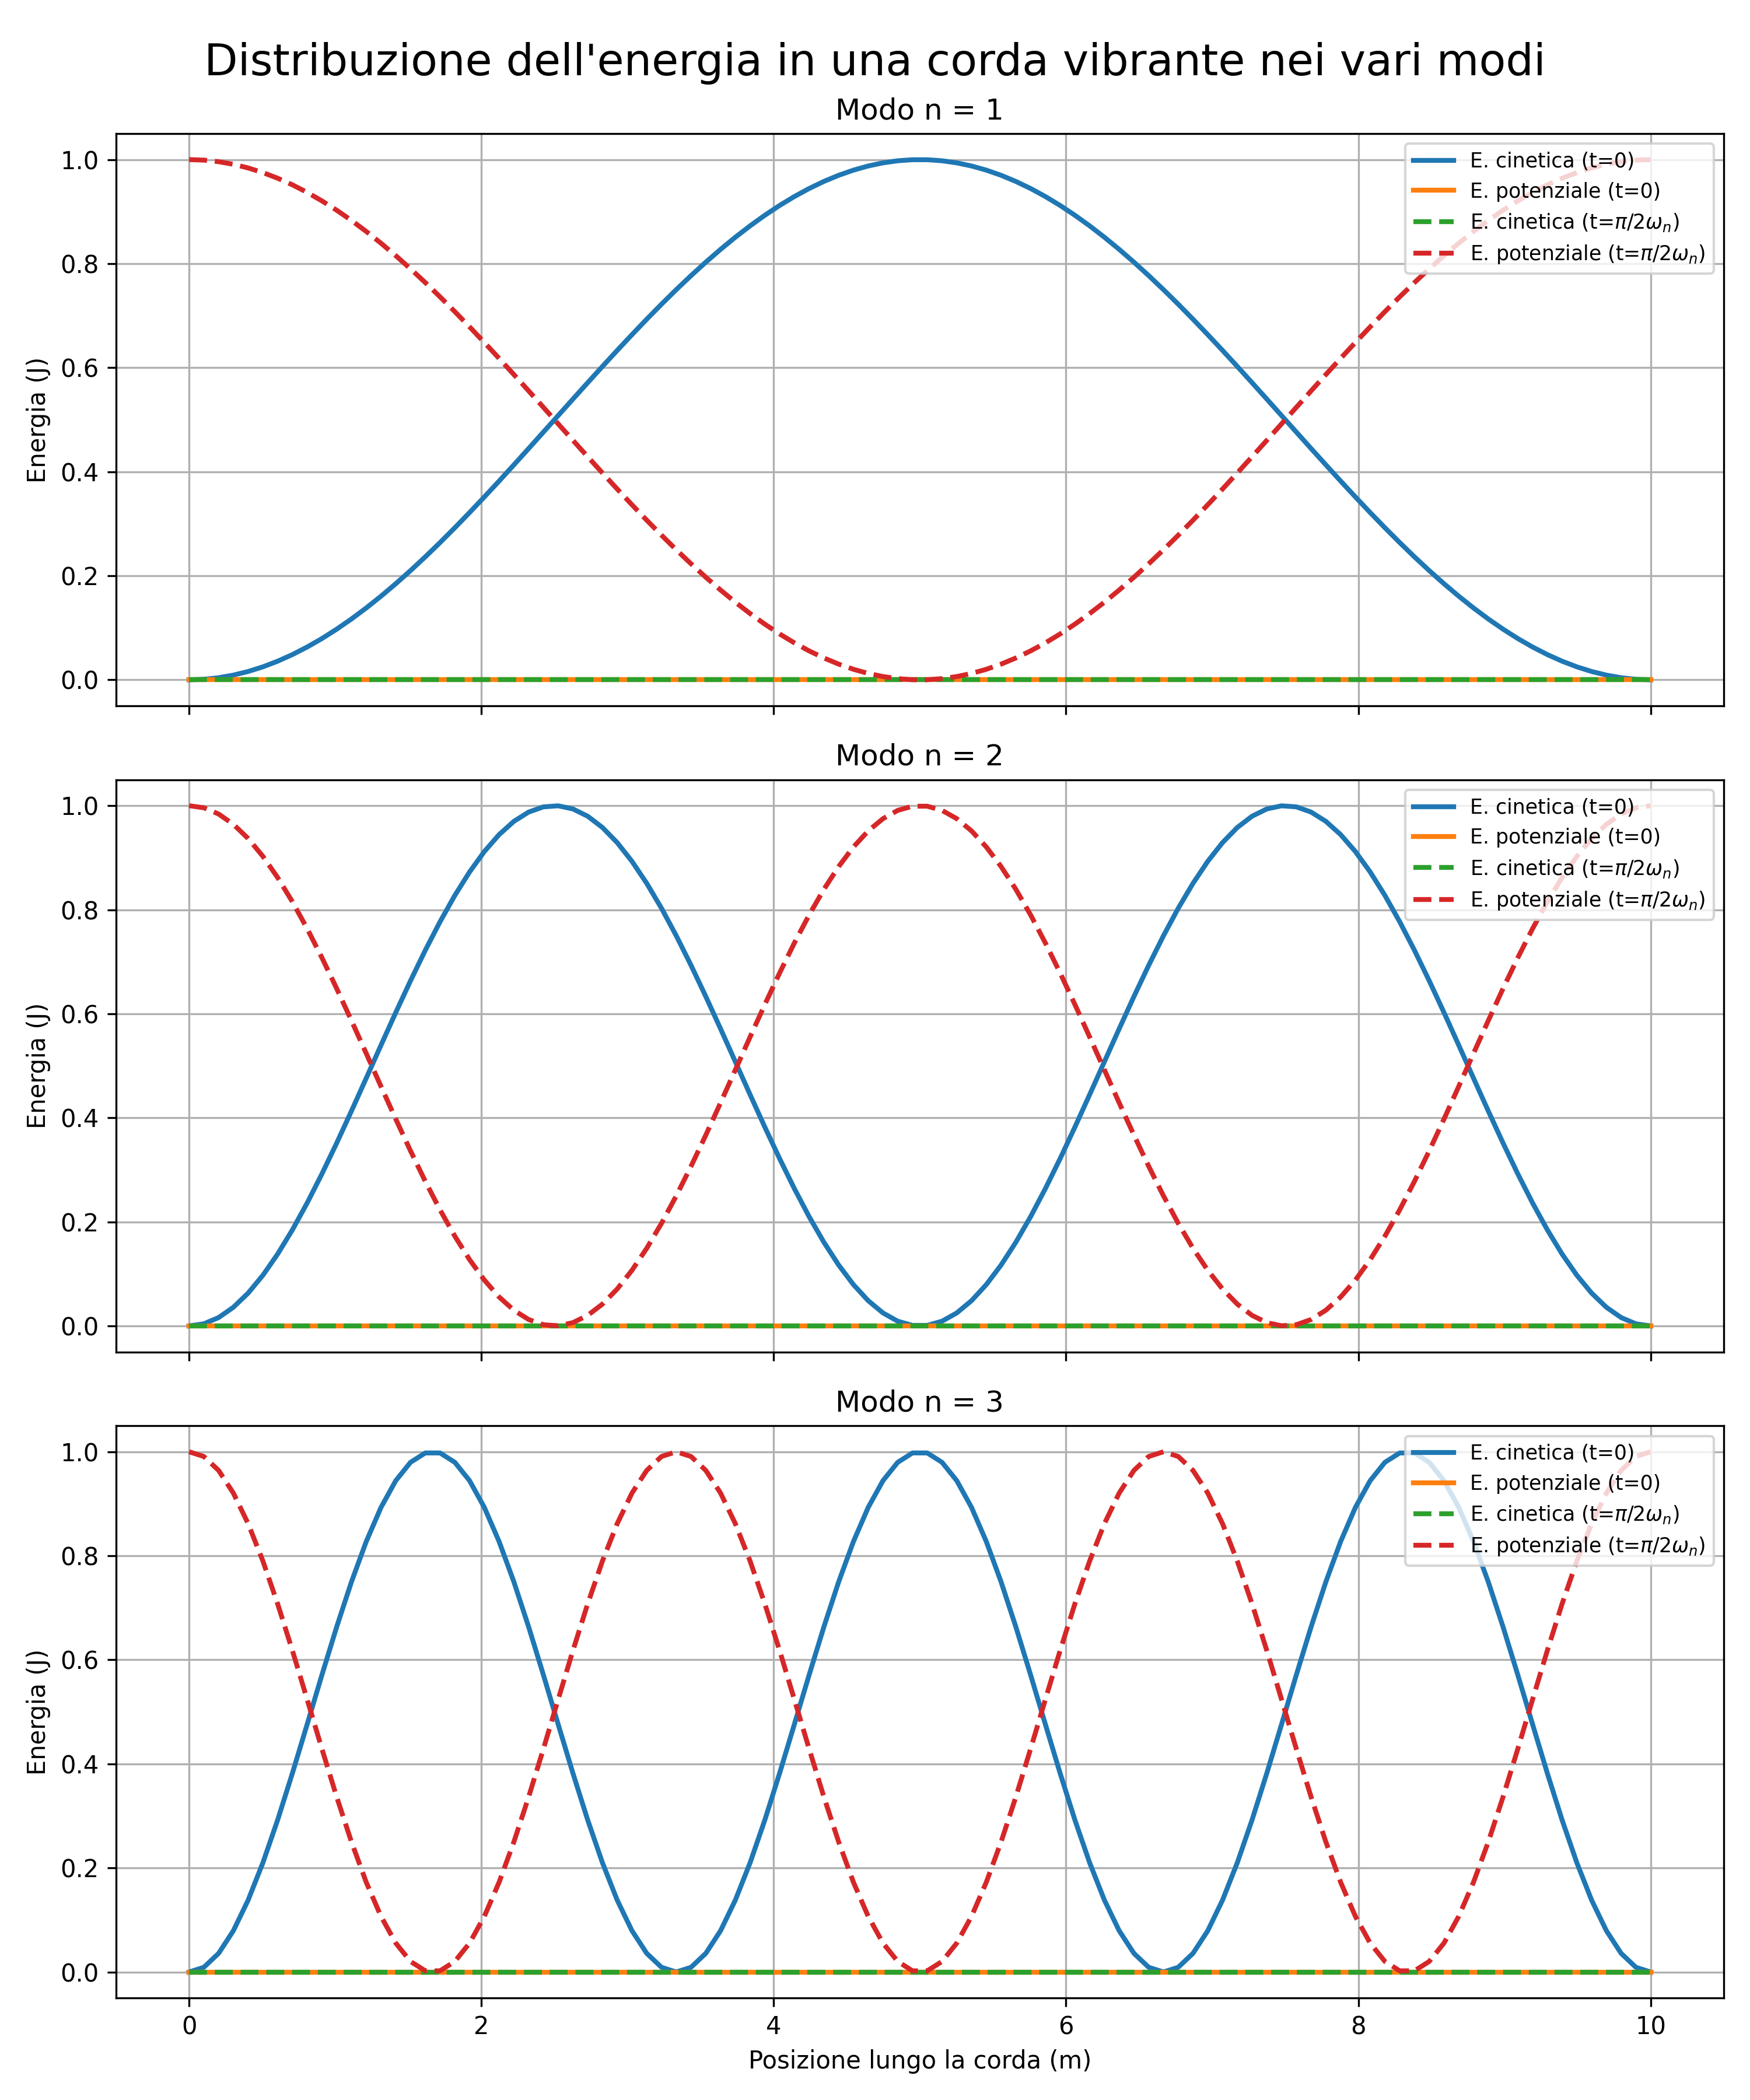
\includegraphics[width=0.75\linewidth]{img/energiaOnde.png}
    \caption{Energia cinetica e potenziale al variare di $n$}
    \label{fig:energiaOnde}
\end{figure}

Pertanto:
\begin{itemize}
    \item negli istanti in cui $\sin(\omega_n t) = 0$ e quindi $\xi = 0; \quad \forall t$, vale:
    \begin{itemize}
        \item Energia potenziale nulla
        \item Energia cinetica massima
    \end{itemize}
    \item negli istanti in cui $\cos(k_n t) = 0$ e quindi $\xi$ è massima per ogni x vale:
    \begin{itemize}
        \item Energia potenziale massima
        \item Energia cinetica nulla
    \end{itemize}
\end{itemize}

\end{document}